% Options for packages loaded elsewhere
\PassOptionsToPackage{unicode}{hyperref}
\PassOptionsToPackage{hyphens}{url}
%
\documentclass[
]{report}
\usepackage{amsmath,amssymb}
\usepackage{iftex}
\ifPDFTeX
  \usepackage[T1]{fontenc}
  \usepackage[utf8]{inputenc}
  \usepackage{textcomp} % provide euro and other symbols
\else % if luatex or xetex
  \usepackage{unicode-math} % this also loads fontspec
  \defaultfontfeatures{Scale=MatchLowercase}
  \defaultfontfeatures[\rmfamily]{Ligatures=TeX,Scale=1}
\fi
\usepackage{lmodern}
\ifPDFTeX\else
  % xetex/luatex font selection
\fi
% Use upquote if available, for straight quotes in verbatim environments
\IfFileExists{upquote.sty}{\usepackage{upquote}}{}
\IfFileExists{microtype.sty}{% use microtype if available
  \usepackage[]{microtype}
  \UseMicrotypeSet[protrusion]{basicmath} % disable protrusion for tt fonts
}{}
\makeatletter
\@ifundefined{KOMAClassName}{% if non-KOMA class
  \IfFileExists{parskip.sty}{%
    \usepackage{parskip}
  }{% else
    \setlength{\parindent}{0pt}
    \setlength{\parskip}{6pt plus 2pt minus 1pt}}
}{% if KOMA class
  \KOMAoptions{parskip=half}}
\makeatother
\usepackage{xcolor}
\usepackage{color}
\usepackage{fancyvrb}
\newcommand{\VerbBar}{|}
\newcommand{\VERB}{\Verb[commandchars=\\\{\}]}
\DefineVerbatimEnvironment{Highlighting}{Verbatim}{commandchars=\\\{\}}
% Add ',fontsize=\small' for more characters per line
\usepackage{framed}
\definecolor{shadecolor}{RGB}{248,248,248}
\newenvironment{Shaded}{\begin{snugshade}}{\end{snugshade}}
\newcommand{\AlertTok}[1]{\textcolor[rgb]{0.94,0.16,0.16}{#1}}
\newcommand{\AnnotationTok}[1]{\textcolor[rgb]{0.56,0.35,0.01}{\textbf{\textit{#1}}}}
\newcommand{\AttributeTok}[1]{\textcolor[rgb]{0.13,0.29,0.53}{#1}}
\newcommand{\BaseNTok}[1]{\textcolor[rgb]{0.00,0.00,0.81}{#1}}
\newcommand{\BuiltInTok}[1]{#1}
\newcommand{\CharTok}[1]{\textcolor[rgb]{0.31,0.60,0.02}{#1}}
\newcommand{\CommentTok}[1]{\textcolor[rgb]{0.56,0.35,0.01}{\textit{#1}}}
\newcommand{\CommentVarTok}[1]{\textcolor[rgb]{0.56,0.35,0.01}{\textbf{\textit{#1}}}}
\newcommand{\ConstantTok}[1]{\textcolor[rgb]{0.56,0.35,0.01}{#1}}
\newcommand{\ControlFlowTok}[1]{\textcolor[rgb]{0.13,0.29,0.53}{\textbf{#1}}}
\newcommand{\DataTypeTok}[1]{\textcolor[rgb]{0.13,0.29,0.53}{#1}}
\newcommand{\DecValTok}[1]{\textcolor[rgb]{0.00,0.00,0.81}{#1}}
\newcommand{\DocumentationTok}[1]{\textcolor[rgb]{0.56,0.35,0.01}{\textbf{\textit{#1}}}}
\newcommand{\ErrorTok}[1]{\textcolor[rgb]{0.64,0.00,0.00}{\textbf{#1}}}
\newcommand{\ExtensionTok}[1]{#1}
\newcommand{\FloatTok}[1]{\textcolor[rgb]{0.00,0.00,0.81}{#1}}
\newcommand{\FunctionTok}[1]{\textcolor[rgb]{0.13,0.29,0.53}{\textbf{#1}}}
\newcommand{\ImportTok}[1]{#1}
\newcommand{\InformationTok}[1]{\textcolor[rgb]{0.56,0.35,0.01}{\textbf{\textit{#1}}}}
\newcommand{\KeywordTok}[1]{\textcolor[rgb]{0.13,0.29,0.53}{\textbf{#1}}}
\newcommand{\NormalTok}[1]{#1}
\newcommand{\OperatorTok}[1]{\textcolor[rgb]{0.81,0.36,0.00}{\textbf{#1}}}
\newcommand{\OtherTok}[1]{\textcolor[rgb]{0.56,0.35,0.01}{#1}}
\newcommand{\PreprocessorTok}[1]{\textcolor[rgb]{0.56,0.35,0.01}{\textit{#1}}}
\newcommand{\RegionMarkerTok}[1]{#1}
\newcommand{\SpecialCharTok}[1]{\textcolor[rgb]{0.81,0.36,0.00}{\textbf{#1}}}
\newcommand{\SpecialStringTok}[1]{\textcolor[rgb]{0.31,0.60,0.02}{#1}}
\newcommand{\StringTok}[1]{\textcolor[rgb]{0.31,0.60,0.02}{#1}}
\newcommand{\VariableTok}[1]{\textcolor[rgb]{0.00,0.00,0.00}{#1}}
\newcommand{\VerbatimStringTok}[1]{\textcolor[rgb]{0.31,0.60,0.02}{#1}}
\newcommand{\WarningTok}[1]{\textcolor[rgb]{0.56,0.35,0.01}{\textbf{\textit{#1}}}}
\usepackage{longtable,booktabs,array}
\usepackage{calc} % for calculating minipage widths
% Correct order of tables after \paragraph or \subparagraph
\usepackage{etoolbox}
\makeatletter
\patchcmd\longtable{\par}{\if@noskipsec\mbox{}\fi\par}{}{}
\makeatother
% Allow footnotes in longtable head/foot
\IfFileExists{footnotehyper.sty}{\usepackage{footnotehyper}}{\usepackage{footnote}}
\makesavenoteenv{longtable}
\usepackage{graphicx}
\makeatletter
\def\maxwidth{\ifdim\Gin@nat@width>\linewidth\linewidth\else\Gin@nat@width\fi}
\def\maxheight{\ifdim\Gin@nat@height>\textheight\textheight\else\Gin@nat@height\fi}
\makeatother
% Scale images if necessary, so that they will not overflow the page
% margins by default, and it is still possible to overwrite the defaults
% using explicit options in \includegraphics[width, height, ...]{}
\setkeys{Gin}{width=\maxwidth,height=\maxheight,keepaspectratio}
% Set default figure placement to htbp
\makeatletter
\def\fps@figure{htbp}
\makeatother
\setlength{\emergencystretch}{3em} % prevent overfull lines
\providecommand{\tightlist}{%
  \setlength{\itemsep}{0pt}\setlength{\parskip}{0pt}}
\setcounter{secnumdepth}{5}
\newlength{\cslhangindent}
\setlength{\cslhangindent}{1.5em}
\newlength{\csllabelwidth}
\setlength{\csllabelwidth}{3em}
\newlength{\cslentryspacingunit} % times entry-spacing
\setlength{\cslentryspacingunit}{\parskip}
\newenvironment{CSLReferences}[2] % #1 hanging-ident, #2 entry spacing
 {% don't indent paragraphs
  \setlength{\parindent}{0pt}
  % turn on hanging indent if param 1 is 1
  \ifodd #1
  \let\oldpar\par
  \def\par{\hangindent=\cslhangindent\oldpar}
  \fi
  % set entry spacing
  \setlength{\parskip}{#2\cslentryspacingunit}
 }%
 {}
\usepackage{calc}
\newcommand{\CSLBlock}[1]{#1\hfill\break}
\newcommand{\CSLLeftMargin}[1]{\parbox[t]{\csllabelwidth}{#1}}
\newcommand{\CSLRightInline}[1]{\parbox[t]{\linewidth - \csllabelwidth}{#1}\break}
\newcommand{\CSLIndent}[1]{\hspace{\cslhangindent}#1}
\usepackage{booktabs}
\usepackage{geometry}
\usepackage[none]{hyphenat}
\usepackage{titlesec}
\usepackage{longtable}
\usepackage{xcolor}
\usepackage{setspace}
\usepackage{pdfpages}

\pagestyle{plain}

%%%% Set margins
\setlength{\topmargin}{-1cm}
\addtolength{\evensidemargin}{-1cm}
\addtolength{\oddsidemargin}{-1cm}
\addtolength{\textheight}{3cm}
\addtolength{\textwidth}{2cm}

% Spacing for reading guides
\newcommand{\rgs}{\vspace{12pt}} % Vertical space
\newcommand{\rgi}{\hspace{24pt}}  % Indent

\newcommand\latexcode[1]{#1}

% Format chapter titles and spacing
\renewcommand*{\chaptername}{Week}

\titleformat{\chapter}[display]
{\bfseries\Large}
{\filleft\MakeUppercase{\chaptertitlename} \Huge\thechapter}
{3ex}
{\titlerule
\vspace{1.5ex}%
\filright}
[\vspace{1.5ex}%
\titlerule]
\titlespacing*{\chapter}{0pt}{-40pt}{20pt}
\ifLuaTeX
  \usepackage{selnolig}  % disable illegal ligatures
\fi
\IfFileExists{bookmark.sty}{\usepackage{bookmark}}{\usepackage{hyperref}}
\IfFileExists{xurl.sty}{\usepackage{xurl}}{} % add URL line breaks if available
\urlstyle{same}
\hypersetup{
  hidelinks,
  pdfcreator={LaTeX via pandoc}}

\title{\textbf{STAT 216 Coursepack}\\
\strut \\
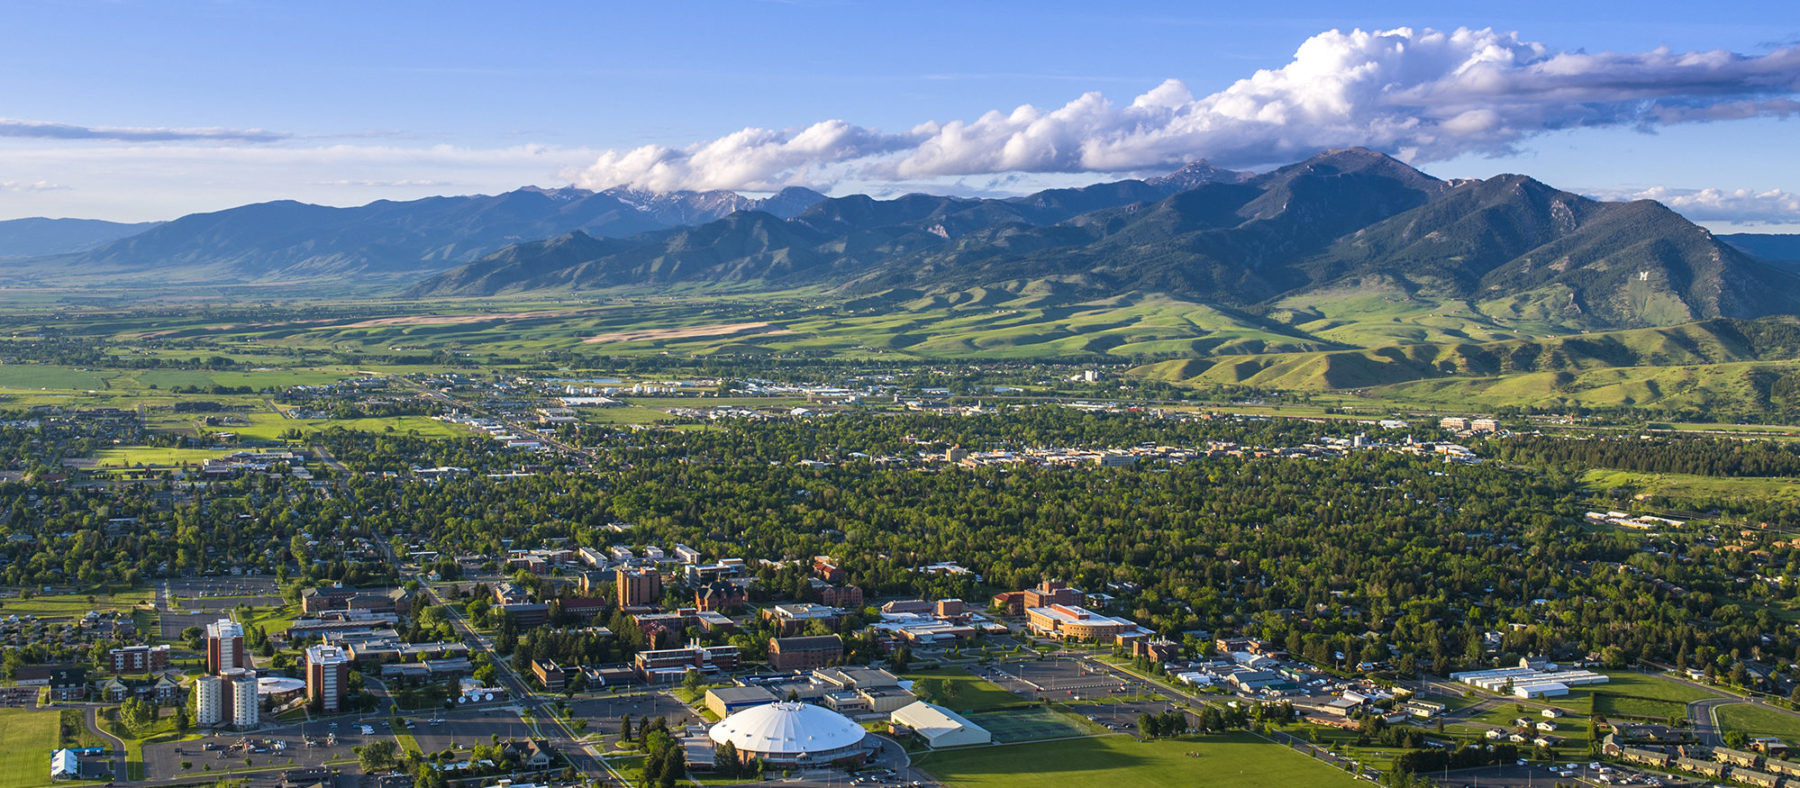
\includegraphics[width=5in,height=\textheight]{images/msu-campus.jpg}}
\usepackage{etoolbox}
\makeatletter
\providecommand{\subtitle}[1]{% add subtitle to \maketitle
  \apptocmd{\@title}{\par {\large #1 \par}}{}{}
}
\makeatother
\subtitle{Spring 2024\\
Montana State University}
\author{Melinda Yager\\
Jade Schmidt\\
Stacey Hancock}
\date{}

\begin{document}
\maketitle

\newpage
\thispagestyle{empty}

This resource was developed by Melinda Yager, Jade Schmidt, and Stacey Hancock in 2021 to accompany the online textbook: Hancock, S., Carnegie, N., Meyer, E., Schmidt, J., and Yager, M. (2021). \emph{Montana State Introductory Statistics with R}. Montana State University. \url{https://mtstateintrostats.github.io/IntroStatTextbook/}.

This resource is released under a \href{https://creativecommons.org/licenses/by-nc-sa/4.0/}{Creative Commons BY-NC-SA 4.0} license unless otherwise noted.

\setcounter{tocdepth}{1}
\addtocontents{toc}{\protect\thispagestyle{empty}}
\tableofcontents
\thispagestyle{empty}

\newpage
\setcounter{page}{1}

\hypertarget{preface}{%
\chapter*{Preface}\label{preface}}
\addcontentsline{toc}{chapter}{Preface}

This coursepack accompanies the textbook for STAT 216: Montana State Introductory Statistics with R, which can be found at \url{https://mtstateintrostats.github.io/IntroStatTextbook/}. The syllabus for the course (including the course calendar), data sets, and links to D2L Brightspace, Gradescope, and the MSU RStudio server can be found on the course webpage: \url{https://math.montana.edu/courses/s216/}.
Other notes and review materials are linked in D2L.

Each of the activities in this workbook is designed to target specific learning outcomes of the course, giving you practice with important statistical concepts in a group setting with instructor guidance. In addition to the in-class activities for the course, reading guides are provided on D2L to aid in taking notes while you complete the required readings. Bring this workbook with you to class each class period, and take notes in the workbook as you would your own notes. A well-written completed workbook will provide an optimal study guide for exams!

The out-of-class activities will be completed outside of class, typically between the Monday and Wednesday classes. The additional activities and labs in this coursepack will be completed during class time. Parts of each lab will be turned in on Gradescope. To aid in your understanding, read through the introduction for each activity before attending class each day.

STAT 216 is a 3-credit in-person course. In our experience, it takes six to nine hours per week outside of class to achieve a good grade in this class. By ``good'' we mean at least a C because a grade of D or below does not count toward fulfilling degree requirements. Many of you set your goals higher than just getting a C, and we fully support that. You need roughly nine hours per week to review past activities, read feedback on previous assignments, complete current assignments, and prepare for the next day's class. A typical week in the life of a STAT 216 student looks like:

\begin{itemize}
\tightlist
\item
  \emph{Prior to class meeting}:

  \begin{itemize}
  \tightlist
  \item
    Read assigned sections of the textbook, using the provided reading guides to take notes on the material.
  \item
    Read through the introduction to the day's in-class activity.
  \item
    Read through the week's homework assignment and note any questions you may have on the content.
  \end{itemize}
\item
  \emph{During class meeting}:

  \begin{itemize}
  \tightlist
  \item
    Fill in the lecture notes during class.
  \item
    Work through the in-class activity or weekly lab with your classmates and instructor, taking detailed notes on your answers to each question in the activity.
  \end{itemize}
\item
  \emph{After class meeting}:

  \begin{itemize}
  \tightlist
  \item
    Complete any parts of the activity you did not complete in class.
  \item
    Review the activity solutions in the Math and Stat Center, and take notes on key points.
  \item
    Complete any remaining assigned readings for the week.
  \item
    Complete the week's homework assignment.
  \end{itemize}
\end{itemize}

\nocite{*}

\hypertarget{spring-2024-calendar-of-coursepack-activities}{%
\chapter*{Spring 2024 Calendar of Coursepack Activities}\label{spring-2024-calendar-of-coursepack-activities}}
\addcontentsline{toc}{chapter}{Spring 2024 Calendar of Coursepack Activities}

This calendar only lists the lectures, the in-class and out-of-class activities, RStudio labs and exams each week. For required readings as well as due dates for assignments, refer to the calendar at:\\
\url{https://mtstateintrostats.github.io/Syllabus/\#Course_calendar}

\begin{longtable}{|l|l|l|l|p{.55\textwidth}|}
\hline
\textbf{Week}& \textbf{Day}& \textbf{Date}& \textbf{Activity} \\ \hline
\endhead

1& W& 1/17& Intro to Data \\*
1& F& 1/19& Data Lecture \\ \hline
2& M& 1/22& Study Design Lecture \\*
2& W& 1/24& Complete Out-of-Class Activity Week 2 \\*
2& W& 1/24& American Indian Address Part 2 \\* 
2& F& 1/26& Week 2 Lab \\ \hline
3& M& 1/29& Categorical and Quantitative EDA Lecture \\*
3& W& 1/31& Complete Out-of-Class Activity Week 3 \\*
3& W& 1/31& Activity 3 \\*
3& F& 2/2& Week 3 Lab \\ \hline
4& M& 2/5& Regression Lecture \\*
4& W& 2/7& Complete Out-of-Class Activity Week 4 \\*
4& W& 2/7& Movie Profits \\*
4& F& 2/9& Week 4 Lab \\ \hline
5& M& 2/12& Exam 1 Review \\*
5& W& 2/14& Group Midterm Exam 1 \\*    
5& F& 2/16& Midterm Exam 1 \\ \hline
6& M& 2/19& (\textit{No class}) \\*
6& W& 2/21& Hypothesis Testing Lecture  \\*
6& F& 2/23& Complete Out-of-Class Activity Week 6 \\*   
6& F& 2/23& Week 6 Lab \\ \hline
7& M& 2/26& Theory-based Testing Lecture \\*
7& W& 2/28& Complete Out-of-Class Activity Week 7 \\*
7& W& 2/28& Handedness of Male Boxers --- Theory \\*
7& F& 3/1& Week 7 Lab \\ \hline
8& M& 3/4& Two Proportion Simulation Lecture \\*
8& W& 3/6& Complete Out-of-Class Activity Week 8 \\*
8& W& 3/6& Good Samaritan --- Simulation HT and CI \\*  
8& F& 3/8& Week 8 Lab \\ \hline
Holiday& M--F& 3/11--3/15& \textbf{No Class --- Spring Break} \\ \hline
9& M& 3/18& Two Proportion Theory Lecture \\*
9& W& 3/20& Complete Out-of-Class Activity Week 9 \\*
9& W& 3/20& Helmet Use and Head Injuries --- Theory HT and CI \\*   
9& F& 3/22& Week 9 Lab \\ \hline
10& M& 3/25& Probability and Relative Risk Lecture \\*
10& W& 3/27& Complete Out-of-Class Activity Week 10 \\*
10& W& 3/27& Relative Risk \\*
10& F& 3/29& (\textit{No class}) \\ \hline
11& M& 4/1& Exam 2 Review \\*
11& W& 4/3& Group Midterm Exam 2 \\*
11& F& 4/5& Midterm Exam 2\\ \hline
12& M& 4/8& Paired Inference Lecture \\*
12& W& 4/10& Complete Out-of-Class Activity Week 12 \\*
12& W& 4/10& Color Interference \\* 
12& F& 4/12& Week 12 Lab \\ \hline
13& M& 4/15& Two Independent Samples Inference Lecture \\*
13& W& 4/17& Complete Out-of-Class Activity Week 13 \\*
13& W& 4/17& Triple Crown \\*
13& F& 4/19& Week 13 Lab \\ \hline
14& M& 4/22& Regression Inference Lecture \\*
14& W& 4/24& Complete Out-of-Class Activity Week 14 \\*
14& W& 4/24& Golf Driving Distances \\*
14& F& 4/26& Week 14 Lab \\ \hline
15& M& 4/29& Final Exam Review \\*
15& W& 5/1& Final Group Exam Part 1 \\*
15& F& 5/3& Final Group Exam Part 2 \\ \hline
Common Final Exam& M--R & 5/6--5/9& See \url{www.montana.edu/registrar/Schedules.html} \\ \hline

\end{longtable}

\nocite{*}

\hypertarget{basics-of-data}{%
\chapter{Basics of Data}\label{basics-of-data}}

\hypertarget{activity-1-intro-to-data}{%
\section{Activity 1: Intro to Data}\label{activity-1-intro-to-data}}

\setstretch{1}

\hypertarget{learning-outcomes}{%
\subsection{Learning outcomes}\label{learning-outcomes}}

\begin{itemize}
\tightlist
\item
  Creating a data set
\end{itemize}

\hypertarget{terminology-review}{%
\subsection{Terminology review}\label{terminology-review}}

Statistics is the study of how best to collect, analyze, and draw conclusions from data. This week in class you will be introduced to the following terms:

\begin{itemize}
\item
  Observational units or cases
\item
  Variables: categorical or quantitative
\end{itemize}

For more on these concepts, read Chapter 1 in the textbook.

\hypertarget{general-information-on-the-coursepack}{%
\subsection{General information on the Coursepack}\label{general-information-on-the-coursepack}}

Information is provided throughout each activity and lab to guide students through that day's activity or lab. Be sure to read ALL the material provided at the beginning of the activity and between each question. At the end of each activity is a section called \emph{Take-home messages} that contains key points from the day's activity. Use these to review the day's activity and make sure you have a full understanding of that material.

\hypertarget{steps-of-the-statistical-investigation-process}{%
\subsection{Steps of the statistical investigation process}\label{steps-of-the-statistical-investigation-process}}

As we move through the semester we will work through the six steps of the statistical investigation process.

\begin{enumerate}
\def\labelenumi{\arabic{enumi}.}
\item
  Ask a research question.
\item
  Design a study and collect data.
\item
  Summarize and visualize the data. \emph{Weeks 3--4}
\item
  Use statistical analysis methods to draw inferences from the data. \emph{Weeks 6--14}
\item
  Communicate the results and answer the research question. \emph{Weeks 6--14}
\item
  Revisit and look forward.
\end{enumerate}

Today we will focus on the first two steps.

\textbf{Step 1}: The first step of any statistical investigation is to \emph{ask a research question}. As stated in the textbook, ``with the rise of data science, however, we might not start with a research question, and instead start with a data set.'' Today we will create a data set by collecting responses on students in class.

\textbf{Step 2}: To answer any research question, we must \emph{design a study and collect data}. Our study will consist of answers from each student. Your responses will become our observed data that we will explore.

\textbf{Observational units} or \textbf{cases} are the subjects data are collected on. In a spreadsheet of the data set, each row will represent a single observational unit.

\newpage

\begin{enumerate}
\def\labelenumi{\arabic{enumi}.}
\tightlist
\item
  One person from each group open the Google sheet linked in D2L and fill in the responses for the following questions for each group member. When creating a data set for use in R it is important to use single words or an underscore between words. Each outcome must be written the same way each time. Make sure to use all lowercase letters to create this data set to have consistency between responses. Do not give units of measure for numerical values within the data set. For \texttt{Residency} use in\_state or out\_state as the two outcomes.
\end{enumerate}

\begin{itemize}
\tightlist
\item
  Major: what is your declared major?
\end{itemize}

\vspace{0.2in}

\begin{itemize}
\tightlist
\item
  Residency: do you have in-state or out-of-state residency?
\end{itemize}

\vspace{0.2in}

\begin{itemize}
\tightlist
\item
  Num\_Credits: how many credits are you taking this semester?
\end{itemize}

\vspace{0.2in}

\begin{itemize}
\tightlist
\item
  Dominant\_hand: are you left or right-handed?
\end{itemize}

\vspace{0.2in}

\begin{itemize}
\tightlist
\item
  Hand\_span: what is the width of your dominant hand from the tip of your thumb to the tip of your pinky with your hand spread out measured in cm?
\end{itemize}

\vspace{0.2in}

\begin{itemize}
\tightlist
\item
  Grip\_dominant: what is the grip strength measured in lbs for your dominant hand?
\end{itemize}

\vspace{0.2in}

\begin{itemize}
\tightlist
\item
  Grip\_nondominant: what is the grip strength measured in lbs for your non-dominant hand?
\end{itemize}

\vspace{0.2in}

\hypertarget{take-home-messages}{%
\subsection{Take-home messages}\label{take-home-messages}}

\begin{enumerate}
\def\labelenumi{\arabic{enumi}.}
\item
  When creating a data set, each row will represent a single observational unit or case. Each column represents a variable collected. It is important to write each variable as a single word or use an underscore between words.
\item
  Make sure to be consistent with writing each outcome in the data set as R is case sensitive. All outcomes must be written exactly the same way.
\end{enumerate}

\hypertarget{additional-notes}{%
\subsection{Additional notes}\label{additional-notes}}

Use this space to summarize your thoughts and take additional notes on today's activity and material covered, and to write down the names and contact information of your teammates.

\newpage

\hypertarget{lecture-notes-week-1-intro-to-data}{%
\section{Lecture Notes Week 1: Intro to data}\label{lecture-notes-week-1-intro-to-data}}

\setstretch{1}

Read through Sections 1.2.1 -- 1.2.5 in the course textbook prior to coming to class on Friday using the reading guides at the beginning of week 1 material.

\hypertarget{data-basics-sections-1.2.1-1.2.2}{%
\subsection*{Data basics: Sections 1.2.1 -- 1.2.2}\label{data-basics-sections-1.2.1-1.2.2}}
\addcontentsline{toc}{subsection}{Data basics: Sections 1.2.1 -- 1.2.2}

Data: \_\_\_\_\_\_\_\_\_\_\_\_\_\_\_\_\_\_\_\_\_\_\_\_\_\_\_\_\_\_\_ used to answer research questions

Observational unit or case: the people or things we \_\_\_\_\_\_\_\_\_\_\_\_\_\_\_\_\_\_\_\_\_ data from

Variable: what is measured on each \_\_\_\_\_\_\_\_\_\_\_\_\_\_\_\_\_ or
\_\_\_\_\_\_\_\_\_\_\_\_\_\_\_\_\_\_.

\hypertarget{types-of-variables}{%
\subsubsection*{Types of variables}\label{types-of-variables}}
\addcontentsline{toc}{subsubsection}{Types of variables}

\begin{itemize}
\tightlist
\item
  Categorical variable:
\end{itemize}

\vspace{0.5in}

\setstretch{1.5}

\rgi - Ordinal: levels of the variable have a natural ordering

\rgi \rgi Examples: `Scale' questions, years of schooling completed

\rgi - Nominal:levels of the variable do not have a natural ordering

\rgi \rgi Examples: hair color, eye color, zipcode

\setstretch{1}

\begin{itemize}
\tightlist
\item
  Quantitative variable:
\end{itemize}

\vspace{0.5in}

\setstretch{1.5}

\rgi - Continuous variables: value can be any value within a range.

\rgi \rgi Examples: percentage of students who are nursing majors

\rgi \rgi \rgi - average hours of exercise per week

\rgi \rgi \rgi - distance or time (measured with enough precision)

\rgi - Discrete variables: can only be specific values, with jumps between

\rgi \rgi Examples: SAT score

\rgi \rgi \rgi - number of car accidents

\setstretch{1}
\newpage

Example for class discussion: The Bureau of Transportation Statistics ({``Bureau of Transportation Statistics''} 2019) collects data on all forms of public transportation. The data set seen here includes several variables collect on flights departing on a random sample of 150 US airports in December of 2019.

\vspace{1mm}

\begin{Shaded}
\begin{Highlighting}[]
\NormalTok{airport }\OtherTok{\textless{}{-}} \FunctionTok{read.csv}\NormalTok{(}\StringTok{"data/airport\_delay.csv"}\NormalTok{)}
\FunctionTok{glimpse}\NormalTok{(airport)}
\CommentTok{\#\textgreater{} Rows: 150}
\CommentTok{\#\textgreater{} Columns: 19}
\CommentTok{\#\textgreater{} $ airport             \textless{}chr\textgreater{} "ABI", "ABY", "ACV", "ACY", "ADQ", "AEX", "ALB", "\textasciitilde{}}
\CommentTok{\#\textgreater{} $ city                \textless{}chr\textgreater{} "Abilene", "Albany", "Arcata/Eureka", "Atlantic Ci\textasciitilde{}}
\CommentTok{\#\textgreater{} $ state               \textless{}chr\textgreater{} " TX", " GA", " CA", " NJ", " AK", " LA", " NY", "\textasciitilde{}}
\CommentTok{\#\textgreater{} $ airport\_name        \textless{}chr\textgreater{} " Abilene Regional", " Southwest Georgia Regional"\textasciitilde{}}
\CommentTok{\#\textgreater{} $ hub                 \textless{}chr\textgreater{} "no", "no", "no", "no", "no", "no", "no", "no", "n\textasciitilde{}}
\CommentTok{\#\textgreater{} $ international       \textless{}chr\textgreater{} "no", "no", "no", "yes", "no", "yes", "yes", "yes"\textasciitilde{}}
\CommentTok{\#\textgreater{} $ elevation\_1000      \textless{}dbl\textgreater{} 1.7906, 0.1932, 0.2223, 0.0748, 0.0787, 0.0881, 0.\textasciitilde{}}
\CommentTok{\#\textgreater{} $ latitude            \textless{}dbl\textgreater{} 32.4, 31.5, 41.0, 39.5, 57.7, 31.3, 42.7, 35.2, 45\textasciitilde{}}
\CommentTok{\#\textgreater{} $ longitude           \textless{}dbl\textgreater{} {-}99.7, {-}81.2, {-}124.1, {-}74.6, {-}152.5, {-}92.5, {-}73.8,\textasciitilde{}}
\CommentTok{\#\textgreater{} $ arr\_flights         \textless{}int\textgreater{} 195, 81, 215, 293, 54, 282, 943, 410, 53, 32314, 6\textasciitilde{}}
\CommentTok{\#\textgreater{} $ perc\_delay15        \textless{}dbl\textgreater{} 16.410256, 13.580247, 23.255814, 15.358362, 12.962\textasciitilde{}}
\CommentTok{\#\textgreater{} $ perc\_cancelled      \textless{}dbl\textgreater{} 0.5128205, 0.0000000, 4.1860465, 0.6825939, 14.814\textasciitilde{}}
\CommentTok{\#\textgreater{} $ perc\_diverted       \textless{}dbl\textgreater{} 0.00000000, 0.00000000, 2.32558139, 0.68259386, 0.\textasciitilde{}}
\CommentTok{\#\textgreater{} $ arr\_delay           \textless{}int\textgreater{} 1563, 1244, 4763, 2905, 329, 1293, 15127, 9705, 25\textasciitilde{}}
\CommentTok{\#\textgreater{} $ carrier\_delay       \textless{}int\textgreater{} 459, 890, 1613, 476, 180, 302, 5627, 2253, 439, 10\textasciitilde{}}
\CommentTok{\#\textgreater{} $ weather\_delay       \textless{}int\textgreater{} 21, 43, 549, 124, 1, 58, 2346, 168, 1236, 13331, 2\textasciitilde{}}
\CommentTok{\#\textgreater{} $ nas\_delay           \textless{}int\textgreater{} 257, 39, 154, 771, 51, 112, 2096, 616, 746, 45674,\textasciitilde{}}
\CommentTok{\#\textgreater{} $ security\_delay      \textless{}int\textgreater{} 0, 0, 0, 25, 0, 0, 44, 0, 0, 375, 0, 83, 0, 23, 0,\textasciitilde{}}
\CommentTok{\#\textgreater{} $ late\_aircraft\_delay \textless{}int\textgreater{} 826, 272, 2447, 1509, 97, 821, 5014, 6668, 108, 10\textasciitilde{}}
\end{Highlighting}
\end{Shaded}

\begin{itemize}
\tightlist
\item
  What are the observational units?
\end{itemize}

\vspace{0.2in}

\begin{itemize}
\tightlist
\item
  Identify which variables are categorical.
\end{itemize}

\vspace{0.2in}

\begin{itemize}
\tightlist
\item
  Identify which variables are quantitative.
\end{itemize}

\vspace{0.2in}

\hypertarget{exploratory-data-analysis-eda}{%
\subsubsection*{Exploratory data analysis (EDA)}\label{exploratory-data-analysis-eda}}
\addcontentsline{toc}{subsubsection}{Exploratory data analysis (EDA)}

Summary statistic: a number which \_\_\_\_\_\_\_\_\_\_\_\_\_\_\_\_\_\_\_\_\_\_\_ an entire data set

\begin{itemize}
\tightlist
\item
  Also called the \_\_\_\_\_\_\_\_\_\_\_ \_\_\_\_\_\_\_\_\_\_\_\_
\end{itemize}

\rgi Examples:

\rgi \rgi proportion of people who had a stroke

\vspace{0.3in}

\rgi \rgi mean (or average) age

\vspace{0.3in}

\begin{itemize}
\tightlist
\item
  The summary statistic and type of plot used depends on the type (categorical or quantitative) of variable(s)!
\end{itemize}

\newpage

\hypertarget{roles-of-variables-sections-1.2.3-1.2.5}{%
\subsection*{Roles of variables: Sections 1.2.3 -- 1.2.5}\label{roles-of-variables-sections-1.2.3-1.2.5}}
\addcontentsline{toc}{subsection}{Roles of variables: Sections 1.2.3 -- 1.2.5}

Explanatory variable: predictor variable

\begin{itemize}
\item
  The variable researchers think \emph{may be} \_\_\_\_\_\_\_\_\_\_\_\_\_
  the other variable.
\item
  In an experiment, what the researchers \_\_\_\_\_\_\_\_\_\_\_\_\_ or \_\_\_\_\_\_\_\_\_\_\_\_\_\_\_\_.
\item
  The groups that we are comparing from the data set.
\end{itemize}

Response variable:

\begin{itemize}
\item
  The variable researchers think \emph{may be} \_\_\_\_\_\_\_\_\_\_\_\_\_\_\_\_\_\_\_ by the other variable.
\item
  Always simply \_\_\_\_\_\_\_\_\_\_\_\_\_\_\_\_ or \_\_\_\_\_\_\_\_\_\_\_\_\_\_\_\_\_\_; never controlled by researchers.
\end{itemize}

Examples for class discussion:

Can you predict a criminal's height based on the footprint left at the scene of a crime?

\begin{itemize}
\tightlist
\item
  Identify the explanatory variable:
\end{itemize}

\vspace{0.25in}

\begin{itemize}
\tightlist
\item
  Identify the response variable:
\end{itemize}

\vspace{0.25in}

Does marking an item on sale (even without changing the price) increase the number of units sold per day, on average?

\begin{itemize}
\tightlist
\item
  Identify the explanatory variable:
\end{itemize}

\vspace{0.25in}

\begin{itemize}
\tightlist
\item
  Identify the response variable:
\end{itemize}

\vspace{0.25in}

In the Physician's Health Study ({``Physician's Health Study,''} n.d.), male physicians participated in a study to determine whether taking a daily low-dose aspirin reduced the risk of heart attacks. The male physicians were randomly assigned to the treatment groups. After five years, 104 of the 11,037 male physicians taking a daily low-dose aspirin had experienced a heart attack while 189 of the 11,034 male physicians taking a placebo had experienced a heart attack.

\begin{itemize}
\tightlist
\item
  Identify the explanatory variable:
\end{itemize}

\vspace{0.25in}

\begin{itemize}
\tightlist
\item
  Identify the response variable:
\end{itemize}

\vspace{0.25in}

\hypertarget{relationships-between-variables}{%
\subsubsection*{Relationships between variables}\label{relationships-between-variables}}
\addcontentsline{toc}{subsubsection}{Relationships between variables}

\setstretch{1.5}

\begin{itemize}
\item
  Association: the \_\_\_\_\_\_\_\_\_\_\_\_\_ between variables create a pattern; knowing something about one variable tells us about the other.

  \begin{itemize}
  \item
    Positive association: as one variable \_\_\_\_\_\_\_\_\_\_\_\_\_, the other tends to \_\_\_\_\_\_\_\_\_\_\_\_\_\_\_ also.
  \item
    Negative association: as one variable \_\_\_\_\_\_\_\_\_\_\_\_\_, the other tends to \_\_\_\_\_\_\_\_\_\_\_\_\_.
  \end{itemize}
\item
  Independent: no clear pattern can be seen between the \_\_\_\_\_\_\_\_\_\_.
\end{itemize}

\setstretch{1}

\hypertarget{further-analysis-of-class-data-set}{%
\subsubsection*{Further analysis of class data set}\label{further-analysis-of-class-data-set}}
\addcontentsline{toc}{subsubsection}{Further analysis of class data set}

\begin{enumerate}
\def\labelenumi{\arabic{enumi}.}
\tightlist
\item
  What are the observational units or cases for the data collected in class on day 1?
\end{enumerate}

\vspace{0.3in}

\begin{enumerate}
\def\labelenumi{\arabic{enumi}.}
\setcounter{enumi}{1}
\tightlist
\item
  How many observations are reported in the data set? This is the \textbf{sample size}.
\end{enumerate}

\vspace{0.3in}

\begin{enumerate}
\def\labelenumi{\arabic{enumi}.}
\setcounter{enumi}{2}
\tightlist
\item
  The header for each column in the data set describes each variable measured on the observational unit.For each column of data, fill in the following table identifying the type of each variable, and if the variable is categorical whether the variables is binary and if the variable is quantitative the units of measure used.
\end{enumerate}

\begin{center}
\begin{tabular}{|l|p{1.5in}|p{0.5in}|p{0.5in}|} \hline
Column & Type of Variable & Binary? & Units? \\ \hline
Major & & &\\
& & & \\ \hline
Residency & & & \\
& & & \\ \hline
Num Credits & & & \\
& & & \\ \hline
Dominant hand & & & \\
& & & \\ \hline
Hand Span & & & \\
& & & \\ \hline
Grip strength dominant hand & & & \\
& & & \\ \hline
Grip strength non-dominant hand & & & \\
& & & \\ \hline
\end{tabular}
\end{center}

\begin{enumerate}
\def\labelenumi{\arabic{enumi}.}
\setcounter{enumi}{3}
\tightlist
\item
  Review the completed data set with your table. Remember that when creating a data set for use in R it is important to use single words or an underscore between words. Each outcome must be written the same way each time to have consistency between responses. Do not give units of measure for numerical values. Write down some issues found with the created class data set.
\end{enumerate}

\newpage

\hypertarget{study-design}{%
\chapter{Study Design}\label{study-design}}

\hypertarget{lecture-notes-week-2-study-design}{%
\section{Lecture Notes Week 2: Study Design}\label{lecture-notes-week-2-study-design}}

\setstretch{1}

\hypertarget{sampling-methods-section-2.1-in-the-course-textbook}{%
\subsection*{Sampling Methods: Section 2.1 in the course textbook}\label{sampling-methods-section-2.1-in-the-course-textbook}}
\addcontentsline{toc}{subsection}{Sampling Methods: Section 2.1 in the course textbook}

\setstretch{1.5}

The method used to collect data will impact

\begin{itemize}
\item
  Target population: all \_\_\_\_\_\_\_\_\_\_\_\_\_\_\_ or \_\_\_\_\_\_\_\_\_\_\_\_\_\_ of interest
\item
  Sample:\_\_\_\_\_\_\_\_\_\_\_\_\_\_\_\_ or \_\_\_\_\_\_\_\_\_\_\_\_\_\_\_\_ from which data is collected
\end{itemize}

\setstretch{1}

Example: Many high schools moved to partial or fully online schooling in Spring of 2020. Did students who graduated in 2020 tend to have a lower GPA during freshman year of college than the previous class of college freshmen? A nationally representative sample of 1000 college students who were freshmen in AY19-20 and 1000 college students who were freshmen in AY20-21 was taken to answer this question.

\begin{itemize}
\tightlist
\item
  What is the target population?
\end{itemize}

\vspace{0.2in}

\begin{itemize}
\tightlist
\item
  What is the sample?
\end{itemize}

\vspace{0.2in}

\hypertarget{good-vs.-bad-sampling}{%
\subsubsection*{Good vs.~bad sampling}\label{good-vs.-bad-sampling}}
\addcontentsline{toc}{subsubsection}{Good vs.~bad sampling}

\setstretch{1.5}

GOAL: to have a sample that is \_\_\_\_\_\_\_\_\_\_\_\_\_\_\_ of the
\_\_\_\_\_\_\_\_\_\_\_\_\_\_ \_\_\_\_\_\_\_\_\_\_\_\_\_\_\_ on the variable(s) of interest

\setstretch{1}

\begin{itemize}
\tightlist
\item
  Unbiased sample methods:
\end{itemize}

\vspace{0.5in}

\rgi \rgi Simple random sample

\begin{itemize}
\tightlist
\item
  Biased sampling method:
\end{itemize}

\vspace{0.5in}

\hypertarget{types-of-sampling-bias}{%
\subsection*{Types of Sampling Bias}\label{types-of-sampling-bias}}
\addcontentsline{toc}{subsection}{Types of Sampling Bias}

\begin{itemize}
\tightlist
\item
  Selection bias:
\end{itemize}

\vspace{0.5in}

\newpage

Example: Newspaper article from 1936 reported that Landon won the presidential election over Roosevelt based on a poll of 10 million voters. Roosevelt was the actual winner. What was wrong with this poll? Poll was completed using a telephone survey and not all people in 1936 had a telephone. Only a certain subset of the population owned a telephone so this subset was over-represented in the telephone survey. The results of the study, showing that Landon would win, did not represent the target population of all US voters.

\begin{itemize}
\tightlist
\item
  Non-response bias:
\end{itemize}

\vspace{0.5in}

\begin{itemize}
\tightlist
\item
  To calculate the non-response rate:
\end{itemize}

\[\frac{\text{number of people who do not respond}}{\text{total number of people selected for the sample}}\times 100\%\]

\begin{itemize}
\tightlist
\item
  For non-response bias to occur must first select people to participate and then they choose not to.
\end{itemize}

Example: A company randomly selects buyers to complete a review of an online purchase but some choose not to respond.

\begin{itemize}
\tightlist
\item
  Response bias:
\end{itemize}

\vspace{0.5in}

Example(s): Police officer pulls you over and asks if you have been drinking. Expect people to say no, whether they have been drinking or not.

\begin{itemize}
\tightlist
\item
  Need to be able to predict how people will respond.
\end{itemize}

Words of caution:

\begin{itemize}
\tightlist
\item
  Convenience samples: gathering data for those who are easily
  accessible; online polls
\end{itemize}

\setstretch{1.5}

\rgi \rgi Selection bias?

\rgi \rgi Non-response bias?

\rgi \rgi Response bias?

\begin{itemize}
\tightlist
\item
  Random sampling reduces \_\_\_\_\_\_\_\_\_\_\_\_\_\_\_\_\_ bias, but
  has no impact on \_\_\_\_\_\_\_\_\_\_\_\_\_\_\_\_ or \_\_\_\_\_\_\_\_\_\_\_\_\_\_ bias.
\end{itemize}

\setstretch{1}

\hypertarget{examples-for-class-discussion}{%
\subsubsection*{Examples for class discussion}\label{examples-for-class-discussion}}
\addcontentsline{toc}{subsubsection}{Examples for class discussion}

A radio talk show asks people to phone in their views on whether the United States should pay off its debt to the United Nations.

\begin{itemize}
\tightlist
\item
  Selection?
\end{itemize}

\vspace{0.25in}

\begin{itemize}
\tightlist
\item
  Non-response?
\end{itemize}

\vspace{0.25in}

\begin{itemize}
\tightlist
\item
  Response?
\end{itemize}

\vspace{0.25in}

The Wall Street Journal plans to make a prediction for the US presidential election based on a survey of its readers and plans to follow-up to ensure everyone responds.

\begin{itemize}
\tightlist
\item
  Selection?
\end{itemize}

\vspace{0.25in}

\begin{itemize}
\tightlist
\item
  Non-response?
\end{itemize}

\vspace{0.25in}

\begin{itemize}
\tightlist
\item
  Response?
\end{itemize}

\vspace{0.25in}

A police detective interested in determining the extent of drug use by high school students, randomly selects a sample of high school students and interviews each one about any illegal drug use by the student during the past year.

\begin{itemize}
\tightlist
\item
  Selection?
\end{itemize}

\vspace{0.25in}

\begin{itemize}
\tightlist
\item
  Non-response?
\end{itemize}

\vspace{0.25in}

\begin{itemize}
\tightlist
\item
  Response?
\end{itemize}

\vspace{0.25in}

\hypertarget{observational-studies-experiments-and-scope-of-inference-sections-2.2-2.4-in-the-course-textbook}{%
\subsection*{Observational studies, experiments, and scope of inference: Sections 2.2 -- 2.4 in the course textbook}\label{observational-studies-experiments-and-scope-of-inference-sections-2.2-2.4-in-the-course-textbook}}
\addcontentsline{toc}{subsection}{Observational studies, experiments, and scope of inference: Sections 2.2 -- 2.4 in the course textbook}

\begin{itemize}
\item
  Review

  \begin{itemize}
  \item
    Explanatory variable: the variable researchers think \emph{may be} effecting the other variable.
  \item
    Response variable: the variable researchers think \emph{may be} influenced by the other variable.
  \end{itemize}
\item
  Confounding variable:

  \begin{itemize}
  \tightlist
  \item
    associated with both the explanatory and the response variable
  \item
    explains the association shown by the data
  \end{itemize}
\end{itemize}

Example:

\vspace{0.8in}

\hypertarget{study-design-1}{%
\subsubsection*{Study design}\label{study-design-1}}
\addcontentsline{toc}{subsubsection}{Study design}

\begin{itemize}
\tightlist
\item
  Observational study:
\end{itemize}

\vspace{0.5in}

\begin{itemize}
\tightlist
\item
  Experiment:
\end{itemize}

\vspace{0.5in}

Principles of experimental design

\begin{itemize}
\item
  Control: hold other differences constant across groups
  \vspace{0.1in}
\item
  Randomization: randomized experiment
  \vspace{0.1in}
\item
  Replication: large sample size or repeat of study
  \vspace{0.1in}
\item
  Blocking: group based on certain characteristics
\end{itemize}

\vspace{0.1in}

Example: It is well known that humans have more difficulty differentiating between faces of people from different races than people within their own race. A 2018 study published in the Journal of Experimental Psychology (Levin 2000): Human Perception and Performance investigated a similar phenomenon with gender. In the study, volunteers were shown several pictures of strangers. Half the volunteers were randomly assigned to rate the attractiveness of the individuals pictured. The other half were told to rate the distinctiveness of the faces seen. Both groups were then shown a slideshow of faces (some that had been rated in the first part of the study, some that were new to the volunteer) and asked to determine if each face was old or new. Researchers found people were better able to recognize faces of their own gender when asked to rate the distinctiveness of the faces, compared to when asked to rate the attractiveness of the faces.

\begin{itemize}
\tightlist
\item
  What is the study design?
\end{itemize}

\vspace{0.5in}

Example: In the Physician's Health Study ({``Physician's Health Study,''} n.d.), male physicians participated in a study to determine whether taking a daily low-dose aspirin reduced the risk of heart attacks. The male physicians were randomly assigned to the treatment groups. After five years, 104 of the 11,037 male physicians taking a daily low-dose aspirin had experienced a heart attack while 189 of the 11,034 male physicians taking a placebo had experienced a heart attack.

\begin{itemize}
\tightlist
\item
  What is the study design?
\end{itemize}

\vspace{0.5in}

\begin{itemize}
\tightlist
\item
  Assuming these data provide evidence that the low-dose aspirin group had a lower rate of heart attacks than the placebo group, is it valid for the researchers to conclude the lower rate of heart attacks was caused by the daily low-dose aspirin regimen?
\end{itemize}

\vspace{0.5in}

\hypertarget{scope-of-inference}{%
\subsubsection*{Scope of Inference}\label{scope-of-inference}}
\addcontentsline{toc}{subsubsection}{Scope of Inference}

\begin{enumerate}
\def\labelenumi{\arabic{enumi}.}
\tightlist
\item
  How was the sample selected?
\end{enumerate}

\begin{itemize}
\tightlist
\item
  Random sample with no sampling bias:
\end{itemize}

\vspace{0.35in}

\begin{itemize}
\tightlist
\item
  Non-random sample with sampling bias:
\end{itemize}

\vspace{0.35in}

\newpage

\begin{enumerate}
\def\labelenumi{\arabic{enumi}.}
\setcounter{enumi}{1}
\tightlist
\item
  What is the study design?
\end{enumerate}

\begin{itemize}
\tightlist
\item
  Randomized experiment:
\end{itemize}

\vspace{0.35in}

\begin{itemize}
\tightlist
\item
  Observational study:
\end{itemize}

\vspace{0.35in}

Scope of Inference Table:

\begin{center}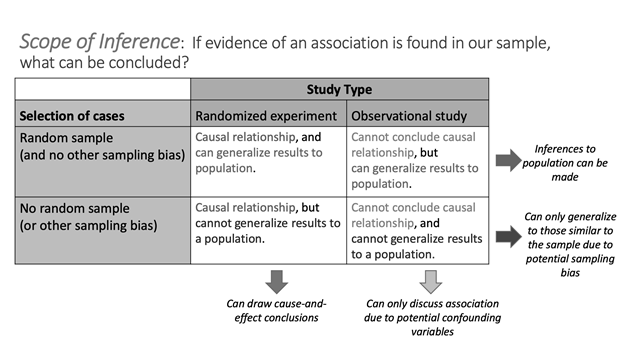
\includegraphics[width=0.75\linewidth]{images/ScopeOfInferenceGreyscale} \end{center}

Example: It is well known that humans have more difficulty differentiating between faces of people from different races than people within their own race. A 2018 study published in the Journal of Experimental Psychology (Levin 2000): Human Perception and Performance investigated a similar phenomenon with gender. In the study, volunteers were shown several pictures of strangers. Half the volunteers were randomly assigned to rate the attractiveness of the individuals pictured. The other half were told to rate the distinctiveness of the faces seen. Both groups were then shown a slideshow of faces (some that had been rated in the first part of the study, some that were new to the volunteer) and asked to determine if each face was old or new. Researchers found people were better able to recognize faces of their own gender when asked to rate the distinctiveness of the faces, compared to when asked to rate the attractiveness of the faces.

\begin{itemize}
\tightlist
\item
  What is the scope of inference for this study?
\end{itemize}

\vspace{0.8in}

Purpose of random assignment:

\vspace{0.8in}

Purpose of random selection:

\newpage
\vspace{0.8in}

\hypertarget{out-of-class-activity-week-2-american-indian-address}{%
\section{Out-of-Class Activity Week 2: American Indian Address}\label{out-of-class-activity-week-2-american-indian-address}}

\setstretch{1}

\hypertarget{learning-outcomes-1}{%
\subsection{Learning outcomes}\label{learning-outcomes-1}}

\begin{itemize}
\item
  Explain why a sampling method is unbiased or biased.
\item
  Identify biased sampling methods.
\item
  Explain the purpose of random selection and its effect on scope of inference.
\end{itemize}

\hypertarget{terminology-review-1}{%
\subsection{Terminology review}\label{terminology-review-1}}

In this activity, we will examine unbiased and biased methods of sampling. Some terms covered in this activity are:

\begin{itemize}
\item
  Random sample
\item
  Unbiased vs biased methods of selection
\item
  Generalization
\end{itemize}

To review these concepts, see Chapter 2 in the textbook.

\hypertarget{american-indian-address}{%
\subsection{American Indian Address}\label{american-indian-address}}

For this activity, you will read a speech given by Jim Becenti, a member of the Navajo American Indian tribe, who spoke about the employment problems his people faced at an Office of Indian Affairs meeting in Phoenix, Arizona, on January 30, 1947 (Moquin and Van Doren 1973). His speech is below:

\textbf{It is hard for us to go outside the reservation where we meet strangers. I have been off the reservation ever since I was sixteen. Today I am sorry I quit the Santa Fe {[}Railroad{]}. I worked for them in 1912--13. You are enjoying life, liberty, and happiness on the soil the American Indian had, so it is your responsibility to give us a hand, brother. Take us out of distress. I have never been to vocational school. I have very little education. I look at the white man who is a skilled laborer. When I was a young man I worked for a man in Gallup as a carpenter's helper. He treated me as his own brother. I used his tools. Then he took his tools and gave me a list of tools I should buy and I started carpentering just from what I had seen. We have no alphabetical language.}

\textbf{We see things with our eyes and can always remember it. I urge that we help my people to progress in skilled labor as well as common labor. The hope of my people is to change our ways and means in certain directions, so they can help you someday as taxpayers. If not, as you are going now, you will be burdened the rest of your life. The hope of my people is that you will continue to help so that we will be all over the United States and have a hand with you, and give us a brotherly hand so we will be happy as you are. Our reservation is awful small. We did not know the capacity of the range until the white man come and say ``you raise too much sheep, got to go somewhere else,'' resulting in reduction to a skeleton where the Indians can't make a living on it. For eighty years we have been confused by the general public, and what is the condition of the Navajo today? Starvation! We are starving for education. Education is the main thing and the only thing that is going to make us able to compete with you great men here talking to us.}

\hypertarget{by-eye-selection}{%
\subsubsection*{By eye selection}\label{by-eye-selection}}
\addcontentsline{toc}{subsubsection}{By eye selection}

\begin{enumerate}
\def\labelenumi{\arabic{enumi}.}
\tightlist
\item
  Circle ten words in Jim Becenti's speech which are a representative sample of the length of words in the entire text. Describe your method for selecting this sample.
\end{enumerate}

\vspace{0.3in}

\begin{enumerate}
\def\labelenumi{\arabic{enumi}.}
\setcounter{enumi}{1}
\tightlist
\item
  Fill in the table below with your selected words from the previous question and the length of each word (number of letters/digits in the word):
  \vspace{1mm}
\end{enumerate}

\begin{center}
\begin{tabular}{|l|p{3in}|p{1in}|} \hline
Observation & Word & Length  \\ \hline
1 & & \\ 
& & \\ \hline
2 & & \\ 
& & \\ \hline
3 & & \\ 
& & \\ \hline
4 & & \\ 
& & \\ \hline
5 & & \\ 
& & \\ \hline
6 & & \\ 
& & \\ \hline
7 & & \\
& & \\ \hline
8 & & \\ 
& & \\ \hline
9 & & \\ 
& & \\ \hline
10 & & \\ 
& & \\ \hline
\end{tabular}
\end{center}

\begin{enumerate}
\def\labelenumi{\arabic{enumi}.}
\setcounter{enumi}{2}
\tightlist
\item
  Calculate the mean (average) word length in your selected sample. Is this value a parameter or a statistic?\\
  \vspace{0.3in}
\end{enumerate}

A dot plot and summary statistics of the ``by-eye'' average word lengths from by-eye samples of size 10 from a Spring 2023 class with 82 students is provided.

\begin{verbatim}
#>   min  Q1 median  Q3  max     mean       sd  n missing
#> 1   3 5.3    6.3 7.5 10.6 6.479268 1.631309 82       0
\end{verbatim}

\begin{center}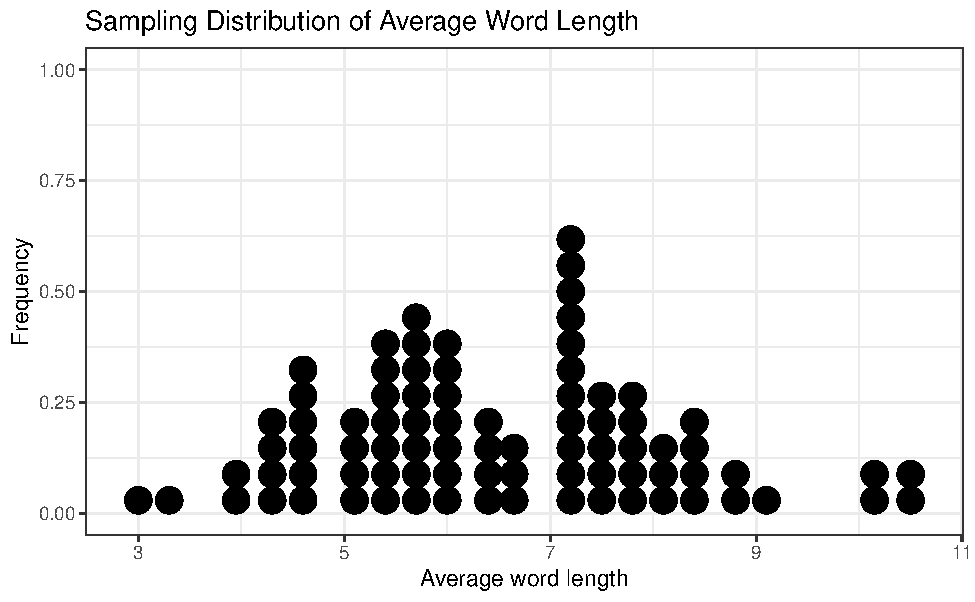
\includegraphics[width=0.7\linewidth]{02-OCA01-bias_files/figure-latex/unnamed-chunk-1-1} \end{center}

\newpage

\begin{enumerate}
\def\labelenumi{\arabic{enumi}.}
\setcounter{enumi}{3}
\item
  Based on the plot and summary statistics of sample mean word lengths, what is your best guess for the average word length of the population of all 359 words in the speech?
  \vspace{0.3in}
\item
  The true mean word length of the population of all 359 words in the speech is 3.95 letters. Is this value a parameter or a statistic?\\
  \vspace{0.2in}

  Where does the value of 3.95 fall in the plot given? Near the center of the distribution? In the tails of the distribution?
  \vspace{0.3in}
\item
  If the class samples were truly representative of the population of words, what proportion of sample means would you expect to be below 3.95?
  \vspace{0.5in}
\item
  Using the graph, estimate the proportion of students' computed sample means that were lower than the true mean of 3.95 letters?
  \vspace{0.5in}
\item
  Based on your answers to questions 6 and 7, would you say the sampling method used by the class is biased or unbiased? Justify your answer.\\
  \vspace{0.5in}
\item
  If the sampling method is biased, what type of sampling bias (selection, response, non-response) is present? What is the direction of the bias, i.e., does the method tend to overestimate or underestimate the population mean word length?
  \vspace{0.5in}
\item
  Should we use results from our ``by eye'' samples to make a statement about the word length in the population of words in Becenti's address? Why or why not?
  \vspace{0.6in}
\end{enumerate}

\newpage

\hypertarget{types-of-bias}{%
\subsubsection*{Types of bias}\label{types-of-bias}}
\addcontentsline{toc}{subsubsection}{Types of bias}

\begin{enumerate}
\def\labelenumi{\arabic{enumi}.}
\setcounter{enumi}{10}
\item
  To determine if the proportion of out-of-state undergraduate students at Montana State University has increased in the last 10 years, a statistics instructor sent an email survey to 500 randomly selected current undergraduate students. One of the questions on the survey asked whether they had in-state or out-of-state residency. She only received 378 responses.
  \vspace{0.1in}

  Sample size:
  \vspace{0.3in}

  Observational units sampled:
  \vspace{0.3in}

  Target population:
  \vspace{0.3in}

  Justify why there is non-response bias in this study.
  \vspace{0.5in}
\item
  A television station is interest in predicting whether or not a local referendum to legalize marijuana for adult use will pass. It asks its viewers to phone in and indicate whether they are in favor or opposed to the referendum. Of the 2241 viewers who phoned in, forty-five percent were opposed to legalizing marijuana.
  \vspace{0.1in}

  Sample size:
  \vspace{0.3in}

  Observational units sampled:
  \vspace{0.3in}

  Target population:
  \vspace{0.3in}

  Justify why there is selection bias in this study.
  \vspace{0.5in}
\end{enumerate}

\newpage

\begin{enumerate}
\def\labelenumi{\arabic{enumi}.}
\setcounter{enumi}{12}
\item
  To gauge the interest in a new swimming pool, a local organization stood outside of the Bogart Pool in Bozeman, MT, during open hours. One of the questions they asked was, ``Since the Bogart Pool is in such bad repair, don't you agree that the city should fund a new pool?''
  \vspace{0.1in}

  Sample size:
  \vspace{0.3in}

  Observational units sampled:
  \vspace{0.3in}

  Target population:
  \vspace{0.3in}

  Justify why there is response bias in this study.
  \vspace{0.5in}

  Justify why there is selection bias in this study.
  \vspace{0.5in}
\item
  The Bozeman school district was interested in surveying parents of students about their opinions on returning to in-person classes following the COVID-19 pandemic. They divided the school district into 10 divisions based on location and randomly surveyed 20 households within each division. Explain why selection bias would be present in this study design.
  \vspace{1in}
\end{enumerate}

\newpage

\hypertarget{take-home-messages-1}{%
\subsection{Take-home messages}\label{take-home-messages-1}}

\begin{enumerate}
\def\labelenumi{\arabic{enumi}.}
\item
  There are three types of bias to be aware of when designing a sampling method: selection bias, non-response bias, and response bias.
\item
  When we use a biased method of selection, we will over or underestimate the parameter.
\item
  To see if a method is biased, we compare the distribution of the estimates to the true value. We want our estimate to be on target or unbiased. When using unbiased methods of selection, the mean of the distribution matches or is very similar to our true parameter.
\item
  If the sampling method is biased, inferences made about the population based on a sample estimate will not be valid.
\end{enumerate}

\hypertarget{additional-notes-1}{%
\subsection{Additional notes}\label{additional-notes-1}}

Use this space to summarize your thoughts and take additional notes on today's activity and material covered.

\newpage

\hypertarget{activity-2-american-indian-address-continued}{%
\section{Activity 2: American Indian Address (continued)}\label{activity-2-american-indian-address-continued}}

\setstretch{1}

\hypertarget{learning-outcomes-2}{%
\subsection{Learning outcomes}\label{learning-outcomes-2}}

\begin{itemize}
\item
  Explain the purpose of random selection and its effect on scope of inference.
\item
  Select a simple random sample from a finite population using a random number generator.
\item
  Explain why a sampling method is unbiased or biased.
\item
  Explain the effect of sample size on sampling variability.
\end{itemize}

\hypertarget{terminology-review-2}{%
\subsection{Terminology review}\label{terminology-review-2}}

In today's activity, we will examine unbiased and biased methods of sampling. Some terms covered in this activity are:

\begin{itemize}
\item
  Random sample
\item
  Unbiased vs biased methods of selection
\item
  Generalization
\end{itemize}

To review these concepts, see Section 2.1 in the textbook.

\hypertarget{random-selection}{%
\subsubsection*{Random selection}\label{random-selection}}
\addcontentsline{toc}{subsubsection}{Random selection}

Today we will return to the American Indian Address introduced in the out-of-class activity. Suppose instead of attempting to select a representative sample by eye (which did not work), each student used a random number generator to select a simple random sample of 10 words. A \textbf{simple random sample} relies on a random mechanism to choose a sample, without replacement, from the population, such that every sample of size 10 is equally likely to be chosen.

To use a random number generator to select a simple random sample, you first need a numbered list of all the words in the population, called a \textbf{sampling frame}. You can then generate 10 random numbers from the numbers 1 to 359 (the number of words in the population), and the chosen random numbers correspond to the chosen words in your sample.

\begin{enumerate}
\def\labelenumi{\arabic{enumi}.}
\tightlist
\item
  Use the random number generator at \url{https://istats.shinyapps.io/RandomNumbers/} to select a simple random sample from the population of all 359 words in the speech.
\end{enumerate}

\begin{itemize}
\item
  Set ``Choose Minimum'' to 1 and ``Choose Maximum'' to 359 to represent the 359 words in the population (the sampling frame).
\item
  Set ``How many numbers do you want to generate?'' to 10 and ensure the ``No'' option is selected under ``Sample with Replacement?''
\item
  Click ``Generate''.
\end{itemize}

\newpage

Fill in the table below with the random numbers selected and use the Becenti.csv data file found on D2L to determine each number's corresponding word and word length (number of letters/digits in the word):

\begin{center}
\begin{tabular}{|l|l|p{1in}|} \hline
Observation & Number & Length  \\ \hline
1 & & \\ 
& & \\ \hline
2 & & \\ 
& & \\ \hline
3 & & \\ 
& & \\ \hline
4 & & \\ 
& & \\ \hline
5 & & \\ 
& & \\ \hline
6 & & \\ 
& & \\ \hline
7 & & \\
& & \\ \hline
8 & & \\ 
& & \\ \hline
9 & &\\ 
& & \\ \hline
10 & & \\ 
& & \\ \hline
\end{tabular}
\end{center}

\begin{enumerate}
\def\labelenumi{\arabic{enumi}.}
\setcounter{enumi}{1}
\tightlist
\item
  Calculate the mean word length in your selected sample in question 1. Is this value a parameter or a statistic?
  \vspace{0.3in}
\end{enumerate}

A dot plot and summary statistics of the average word lengths from random samples of size 10 from a Spring 2023 class of 82 students is provided.

\begin{verbatim}
#>   min  Q1 median    Q3 max     mean        sd  n missing
#> 1 2.5 3.5   3.85 4.375 5.7 3.926829 0.6856643 82       0
\end{verbatim}

\begin{center}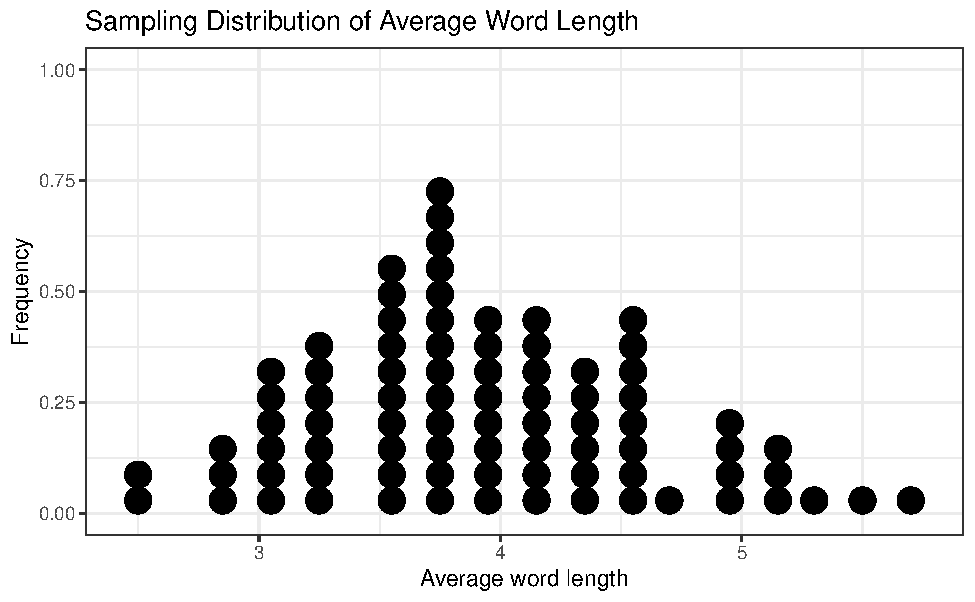
\includegraphics[width=0.7\linewidth]{02-A02-sampling_files/figure-latex/unnamed-chunk-1-1} \end{center}

\newpage

\begin{enumerate}
\def\labelenumi{\arabic{enumi}.}
\setcounter{enumi}{2}
\item
  Where does the value 3.95, the true mean word length, fall in the distribution given? Near the center of the distribution? In the tails of the distribution? Circle this value on the provided distribution.
  \vspace{0.3in}
\item
  How does the plot given in this activity compare to the plot generated in the out-of-class activity?
\end{enumerate}

\rgi Is the shape similar?\\
\vspace{0.2in}

\rgi Is the range (smallest to largest values) similar?

\vspace{0.2in}

\rgi Is the mean of the distribution similar?

\vspace{0.2in}

\rgi Why didn't everyone get the same sample mean?
\vspace{0.4in}

One set of randomly generated sample mean word lengths from a single class may not be large enough to visualize the distribution results. Let's have a computer generate 1,000 sample mean word lengths for us.

\begin{itemize}
\item
  Navigate to the ``One Variable with Sampling'' Rossman/Chance web applet: \url{http://www.rossmanchance.com/applets/2021/sampling/OneSample.html?population=gettysburg}.
\item
  Click ``Clear'' below the text box containing data from the Gettysburg address to delete that data set.
\item
  Download the Becenti.csv file from D2L and open the spreadsheet on your computer.
\item
  Copy and paste the population of word lengths (column C) into the applet from the data set provided making sure to include the header. Click ``Use Data''. Verify that the mean for the data set is 3.953 with a sample size of 359. If these are not the values you got, check with your instructor for help with copying in the data set correctly.
\item
  Click the check-box for ``Show Sampling Options''
\item
  Select 1000 for ``Number of samples'' and select 10 for the ``Sample size''.
\item
  Click ``Draw Samples''.
\end{itemize}

\begin{enumerate}
\def\labelenumi{\arabic{enumi}.}
\setcounter{enumi}{4}
\item
  The plot labeled ``Statistics'' displays the 1,000 randomly generated sample mean word lengths. Sketch this plot below. Include a descriptive \(x\)-axis label and be sure to write down the provided mean and SD (standard deviation) of the distribution.
  \vspace{2in}
\item
  What is the center value (mean) of the distribution created in question 5?
  \vspace{0.3in}
\item
  Explain why the sampling method of using a random number generator to generate a sample is a ``better'' method than choosing 10 words ``by eye''.
  \vspace{0.8in}
\item
  Is random selection an unbiased method of selection? Explain your answer. Be sure to reference your plot from question 5.
  \vspace{0.5in}
\end{enumerate}

\hypertarget{effect-of-sample-size}{%
\subsection*{Effect of sample size}\label{effect-of-sample-size}}
\addcontentsline{toc}{subsection}{Effect of sample size}

We will now consider the impact of sample size.

\begin{enumerate}
\def\labelenumi{\arabic{enumi}.}
\setcounter{enumi}{8}
\item
  First, consider if each student had selected 20 words, instead of 10, by eye. Do you think this would make the plot from the out-of-class activity centered on 3.95 (the true mean word length)? Explain your answer.
  \vspace{0.4in}
\item
  Now we will select 20 words instead of 10 words at random.
\end{enumerate}

\begin{itemize}
\item
  In the ``One Variable with Sampling'' Rossman/Chance web applet(\url{http://www.rossmanchance.com/applets/2021/sampling/OneSample.html?population=gettysburg}.), change the Sample size to 20.
\item
  Click ``Draw Samples''.
\end{itemize}

The plot labeled ``Statistics'' displays the 1,000 randomly generated sample mean word lengths. Sketch this plot below. Include a descriptive \(x\)-axis label and be sure to write down the provided mean and SD (standard deviation) of the distribution.
\vspace{2in}

\begin{enumerate}
\def\labelenumi{\arabic{enumi}.}
\setcounter{enumi}{10}
\tightlist
\item
  Compare the distribution created in question 10 to the one created in question 5.
\end{enumerate}

\rgi Is the shape similar?\\
\vspace{0.2in}

\rgi Is the range (smallest to largest values) similar?

\vspace{0.2in}

\rgi Is the mean of the distribution similar?

\vspace{0.2in}

\begin{enumerate}
\def\labelenumi{\arabic{enumi}.}
\setcounter{enumi}{11}
\item
  Compare the values of the standard deviation of the plots in question 10 and in question 5. Which plot shows the smallest standard deviation?
  \vspace{0.4in}
\item
  Using the evidence from your simulations, answer the following research questions:
\end{enumerate}

\rgi Does changing the sample size impact whether the sample estimates are unbiased? Explain your answer.
\vspace{0.5in}

\rgi Does changing the sample size impact the variability (spread) of sample estimates? Explain your answer
\vspace{0.5in}

\begin{enumerate}
\def\labelenumi{\arabic{enumi}.}
\setcounter{enumi}{13}
\tightlist
\item
  What is the purpose of random selection of a sample from the population?
\end{enumerate}

\vspace{0.8in}

\hypertarget{take-home-messages-2}{%
\subsection{Take-home messages}\label{take-home-messages-2}}

\begin{enumerate}
\def\labelenumi{\arabic{enumi}.}
\item
  Random selection is an unbiased method of selection.
\item
  To determine if a sampling method is biased or unbiased, we compare the distribution of the estimates to the true value. We want our estimate to be on target or unbiased. When using unbiased methods of selection, the mean of the distribution matches or is very similar to our true parameter.
\item
  Random selection eliminates selection bias. However, random selection will not eliminate response or non-response bias.
\item
  The larger the sample size, the more similar (less variable) the statistics will be from different samples.
\item
  Sample size has no impact on whether a \emph{sampling method} is biased or not. Taking a larger sample using a biased method will still result in a sample that is not representative of the population.
\end{enumerate}

\hypertarget{additional-notes-2}{%
\subsection{Additional notes}\label{additional-notes-2}}

Use this space to summarize your thoughts and take additional notes on today's activity and material covered.

\newpage

\hypertarget{week-2-lab-study-design}{%
\section{Week 2 Lab: Study Design}\label{week-2-lab-study-design}}

\setstretch{1}

\hypertarget{learning-outcomes-3}{%
\subsection{Learning outcomes}\label{learning-outcomes-3}}

\begin{itemize}
\item
  Explain the purpose of random assignment and its effect on scope of inference.
\item
  Identify whether a study design is observational or an experiment.
\item
  Identify confounding variables in observational studies and explain why they are confounding.
\end{itemize}

\hypertarget{terminology-review-3}{%
\subsection{Terminology review}\label{terminology-review-3}}

In this activity, we will examine different study designs, confounding variables, and how to determine the scope of inference for a study. Some terms covered in this activity are:

\begin{itemize}
\item
  Scope of inference
\item
  Explanatory variable
\item
  Response variable
\item
  Confounding variable
\item
  Experiment
\item
  Observational study
\end{itemize}

To review these concepts, see Sections 2.2 through 2.5 in the textbook.

\hypertarget{general-information-labs}{%
\subsection{General information labs}\label{general-information-labs}}

At the end of each week you will complete a lab. Questions are selected from each lab to be turned in on Gradescope. The questions to be submitted on Gradescope are bolded in the lab. As you work through the lab have the Gradescope lab assignment open so that you can answer those questions as you go.

\hypertarget{atrial-fibrillation}{%
\subsection{Atrial fibrillation}\label{atrial-fibrillation}}

Atrial fibrillation is an irregular and often elevated heart rate. In some people, atrial fibrillation will come and go on its own, but others will experience this condition on a permanent basis. When atrial fibrillation is constant, medications are required to stabilize the patient's heart rate and to help prevent blood clots from forming. Pharmaceutical scientists at a large pharmaceutical company believe they have developed a new medication that effectively stabilizes heart rates in people with permanent atrial fibrillation. They set out to conduct a trial study to investigate the new drug. The scientists will need to compare the proportion of patients whose heart rate is stabilized between two groups of subjects, one of whom is given a placebo and the other given the new medication.

\begin{enumerate}
\def\labelenumi{\arabic{enumi}.}
\item
  Identify the explanatory and response variable in this trial study.

  Explanatory variable:
  \vspace{0.5in}

  Response variable:
  \vspace{0.5in}
\end{enumerate}

\newpage

Suppose 24 subjects with permanent atrial fibrillation have volunteered to participate in this study. There are 16 subjects that self-identified as male and 8 subjects that self-identified as female.

\begin{enumerate}
\def\labelenumi{\arabic{enumi}.}
\setcounter{enumi}{1}
\item
  One way to separate into two groups would be to give all the males the placebo and all the females the new drug. Explain why this is not a reasonable strategy.
  \vspace{1in}
\item
  Could the scientists fix the problem with the strategy presented in question 2 by creating equal sized groups by putting 4 males and 8 females into the drug group and the remaining 12 males in the placebo group? Explain your answer.
  \vspace{0.5in}
\item
  A third strategy would be to \textbf{block} on sex. In this type of study, the scientists would assign 4 females and 8 males to each group. Using this strategy, out of the 12 individuals in each group what \textbf{proportion} are males?
  \vspace{0.3in}
\item
  \textbf{Assume the scientists used the strategy in question 4, but they put the four tallest females and eight tallest males into the drug group and the remaining subjects into the placebo group. They found that the proportion of patients whose heart rate stabilized is higher in the drug group than the placebo group.}\\
  \vspace{0.1in}

  Could that difference be due to the sex of the subjects? Explain your answer.
  \vspace{0.5in}

  Could it be due to other variables? Explain your answer.
  \vspace{0.5in}
\end{enumerate}

While the strategy presented in question 5 controlled for the sex of the subject, there are more potential \textbf{confounding variables} in the study. A confounding variable is a variable that is \emph{both}

\begin{enumerate}
\def\labelenumi{\arabic{enumi}.}
\tightlist
\item
  associated with the explanatory variable, \emph{and}
\item
  associated with the response variable.
\end{enumerate}

When both these conditions are met, if we observe an association between the explanatory variable and the response variable in the data, we cannot be sure if this association is due to the explanatory variable or the confounding variable---the explanatory and confounding variables are ``confounded.''

\textbf{Random assignment} means that subjects in a study have an equally likely chance of receiving any of the available treatments.

\newpage

\begin{enumerate}
\def\labelenumi{\arabic{enumi}.}
\setcounter{enumi}{5}
\tightlist
\item
  You will now investigate how randomly assigning subjects impacts a study's scope of inference.
\end{enumerate}

\begin{itemize}
\item
  Navigate to the ``Randomizing Subjects'' applet under the ``Other Applets'' heading at: \url{http://www.rossmanchance.com/ISIapplets.html}. This applet lists the sex and height of each of the 24 subjects. Click ``Show Graphs'' to see a bar chart showing the sex of each subject. Currently, the applet is showing the strategy outlined in question 3.
\item
  Click ``Randomize''.
\end{itemize}

~~~In this random assignment, what proportion of males are in group 1 (the placebo group)?

\vspace{0.1in}

~~~What proportion of males are in group 2 (the drug group)?

\vspace{0.1in}

~~~What is the difference in proportion of males between the two groups (placebo - drug)?

\vspace{0.1in}

\begin{enumerate}
\def\labelenumi{\arabic{enumi}.}
\setcounter{enumi}{6}
\item
  Notice the difference in the two proportions is shown as a dot in the plot at the bottom of the web page. Un-check the box for Animate above ``Randomize'' and click ``Randomize'' again. Did you get the same difference in proportion of males between the placebo and drug groups?
  \vspace{0.25in}
\item
  Change ``Replications'' to 998 (for 1000 total). Click ``Randomize'' again. Sketch the plot of the distribution of difference in proportions from each of the 1000 random assignments here. Be sure to include a descriptive \(x\)-axis label.
  \vspace{1.25in}
\item
  \textbf{Does random assignment \emph{always} balance the placebo and drug groups based on the sex of the participants? Does random assignment \emph{tend} to make the placebo and drug groups \emph{roughly} the same with respect to the distribution of sex? Use your plot from question 8 to justify your answers.}
  \vspace{0.5in}
\item
  Change the drop-down menu below Group 2 from ``sex'' to ``height''. The applet now calculates the average height in the placebo and drug groups for each of the 1000 random assignments. The dot plot displays the distribution of the difference in mean heights (placebo - drug) for each random assignment. Based on this dot plot, is height distributed equally, on average, between the two groups? Explain how you know.
  \vspace{0.5in}
\end{enumerate}

\newpage

The diagram below summarizes these ideas about confounding variables and random assignment. When a confounding variable is present (such as sex or height), and an association is found in a study, it is impossible to discern what caused the change in the response variable. Is the change the result of the explanatory variable or the confounding variable? However, if all confounding variables are \emph{balanced} across the treatment groups, then only the explanatory variable differs between the groups and thus \emph{must have caused} the change seen in the response variable.

\begin{center}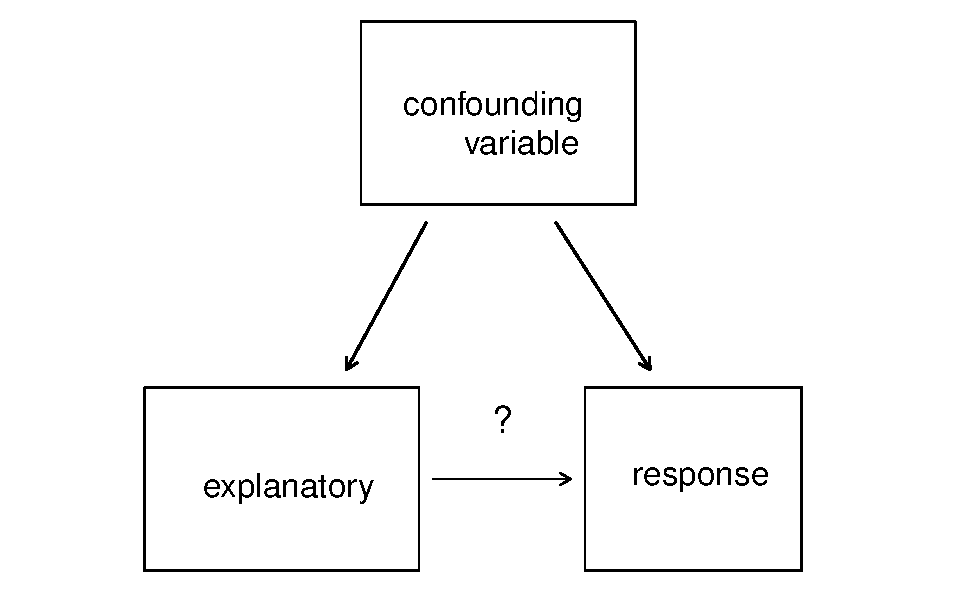
\includegraphics[width=0.4\linewidth]{02-L01-random-assignment_files/figure-latex/unnamed-chunk-1-1} \end{center}

\begin{enumerate}
\def\labelenumi{\arabic{enumi}.}
\setcounter{enumi}{10}
\item
  \textbf{What is the purpose of random assignment of the subjects in a study to the explanatory variable groups?} Cross out the arrow in the figure above that is eliminated by random assignment.
  \vspace{0.8in}
\item
  Suppose in this study on atrial fibrillation, the scientists did randomly assign groups and found that the drug group has a higher proportion of subjects whose heart rates stabilized than the placebo group. Can the scientists conclude the new drug \emph{caused} the increased chance of stabilization? Explain your answer.
  \vspace{0.8in}
\item
  Is the sample of subjects a simple random sample or a convenience sample?
\end{enumerate}

\vspace{0.3in}

\begin{enumerate}
\def\labelenumi{\arabic{enumi}.}
\setcounter{enumi}{13}
\tightlist
\item
  \textbf{Both the sampling method and the study design will help to determine the \emph{scope of inference} for a study: To \emph{whom} can we generalize, and can we conclude \emph{causation or only association}? Use your answers to question 12 and 13 and the table on the next page to determine the scope of inference of this trial study described in question 12.}
  \vspace{0.3in}
\end{enumerate}

\begin{center}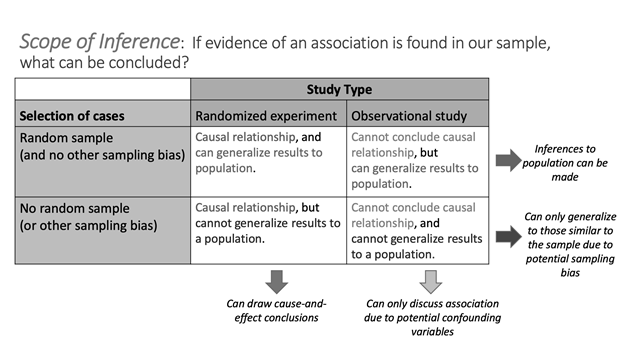
\includegraphics[width=0.75\linewidth]{images/ScopeOfInferenceGreyscale} \end{center}

\hypertarget{study-design-2}{%
\subsection{Study design}\label{study-design-2}}

The two main study designs we will cover are \textbf{observational studies} and \textbf{experiments}. In observational studies, researchers have no influence over which subjects are in each group being compared (though they can control other variables in the study). An experiment is defined by assignment of the treatment groups of the \emph{explanatory variable}, typically via random assignment.

For the next exercises identify the study design (observational study or experiment), the sampling method, and the scope of inference.

\begin{enumerate}
\def\labelenumi{\arabic{enumi}.}
\setcounter{enumi}{14}
\item
  The pharmaceutical company Moderna Therapeutics, working in conjunction with the National Institutes of Health, conducted Phase 3 clinical trials of a vaccine for COVID-19 in the Fall of 2021. US clinical research sites enrolled 30,000 volunteers without COVID-19 to participate. Participants were randomly assigned to receive either the candidate vaccine or a saline placebo. They were then followed to assess whether or not they developed COVID-19. The trial was double-blind, so neither the investigators nor the participants knew who was assigned to which group.
  \vspace{0.1in}

  Study design:
  \vspace{0.3in}

  Sampling method:
  \vspace{0.3in}

  Scope of inference:
  \newpage
\item
  \textbf{In another study, a local health department randomly selected 1000 US adults without COVID-19 to participate in a health survey. Each participant was assessed at the beginning of the study and then followed for one year. They were interested to see which participants elected to receive a vaccination for COVID-19 and whether any participants developed COVID-19.}
  \vspace{0.1in}

  Study design:
  \vspace{0.3in}

  Sampling method:
  \vspace{0.3in}

  Scope of inference:
  \vspace{0.3in}
\end{enumerate}

\hypertarget{take-home-messages-3}{%
\subsection{Take-home messages}\label{take-home-messages-3}}

\begin{enumerate}
\def\labelenumi{\arabic{enumi}.}
\item
  The study design (observational study vs, experiment) determines if we can draw causal inferences or not. If an association is detected, a randomized experiment allows us to conclude that there is a causal (cause-and-effect) relationship between the explanatory and response variable. Observational studies have potential confounding variables within the study that prevent us from inferring a causal relationship between the variables studied.
\item
  Confounding variables are variables not included in the study that are related to both the explanatory and the response variables. When there are potential confounding variables in the study we cannot draw causal inferences.
\item
  Random assignment balances confounding variables across treatment groups. This eliminates any possible confounding variables by breaking the connections between the explanatory variable and the potential confounding variables.
\item
  Observational studies will always carry the possibility of confounding variables. Randomized experiments, which use random assignment, will have no confounding variables.
\end{enumerate}

\hypertarget{additional-notes-3}{%
\subsection{Additional notes}\label{additional-notes-3}}

Use this space to summarize your thoughts and take additional notes on today's activity and material covered.

\newpage

\hypertarget{exploring-categorical-and-quantitative-data}{%
\chapter{Exploring Categorical and Quantitative Data}\label{exploring-categorical-and-quantitative-data}}

\hypertarget{lecture-notes-week-3-exploratory-data-analysis}{%
\section{Lecture Notes Week 3: Exploratory Data Analysis}\label{lecture-notes-week-3-exploratory-data-analysis}}

\setstretch{1}

\hypertarget{summarizing-categorical-data}{%
\subsection*{Summarizing categorical data}\label{summarizing-categorical-data}}
\addcontentsline{toc}{subsection}{Summarizing categorical data}

\begin{itemize}
\item
  A \_\_\_\_\_\_\_\_\_\_\_\_\_\_ is calculated on data from a sample
\item
  The parameter of interest is what we want to know from the population.
\item
  Includes:

  \begin{itemize}
  \item
    Population word (true, long-run, population)
  \item
    Summary measure (depends on the type of data)
  \item
    Context

    \begin{itemize}
    \item
      Observational units
    \item
      Variable(s)
    \end{itemize}
  \end{itemize}
\end{itemize}

Categorical data can be numerically summarized by calculating a \_\_\_\_\_\_\_\_\_\_\_\_\_\_\_ from the data set.

Notation used for the population proportion:

\begin{itemize}
\tightlist
\item
  Single categorical variable:
\end{itemize}

\vspace{0.2in}

\begin{itemize}
\tightlist
\item
  Two categorical variables:
\end{itemize}

\vspace{0.2in}

\rgi \rgi - Subscripts represent the \_\_\_\_\_\_\_\_\_\_\_ variable groups

Notation used for the sample proportion:

\begin{itemize}
\tightlist
\item
  Single categorical variable:
\end{itemize}

\vspace{0.2in}

\begin{itemize}
\tightlist
\item
  Two categorical variables
\end{itemize}

\vspace{0.2in}

\setstretch{1.5}

Categorical data can be reported in a \_\_\_\_\_\_\_\_\_\_\_\_table,
which plots counts or a \_\_\_\_\_\_\_\_\_\_\_\_\_\_
frequency table, which plots the proportion.

When we have two categorical variables we report the data in a \_\_\_\_\_\_\_\_\_\_\_\_\_\_\_ or two-way table with the \_\_\_\_\_\_\_\_\_\_\_\_\_\_\_ variable on the columns and the \_\_\_\_\_\_\_\_\_\_\_\_ variable on the rows.

\setstretch{1}

\vspace{2mm}

Example for class discussion: Gallatin Valley is the fastest growing county in Montana. You'll often hear Bozeman residents complaining about the `out-of-staters' moving in. A local real estate agent recorded data on a random sample of 100 home sales over the last year at her company and noted where the buyers were moving from as well as the age of the person or average age of a couple buying a home. The variable age was binned into two categories, ``Under30'' and ``Over30.'' Additionally, the variable, state the buyers were moving from, was created as a binary variable, ``Out'' for a location out of state and ``In'' for a location in state.

The following code reads in the data set, \texttt{moving\_to\_mt} and names the object moving.

\begin{Shaded}
\begin{Highlighting}[]
\NormalTok{moving }\OtherTok{\textless{}{-}} \FunctionTok{read.csv}\NormalTok{(}\StringTok{"data/moving\_to\_mt.csv"}\NormalTok{)}
\end{Highlighting}
\end{Shaded}

The \texttt{R} function \texttt{glimpse} was used to give the following output.

\begin{Shaded}
\begin{Highlighting}[]
\FunctionTok{glimpse}\NormalTok{(moving)}
\CommentTok{\#\textgreater{} Rows: 100}
\CommentTok{\#\textgreater{} Columns: 4}
\CommentTok{\#\textgreater{} $ From      \textless{}chr\textgreater{} "CA", "CA", "CA", "CA", "CA", "CA", "CA", "CA", "CA", "CA", \textasciitilde{}}
\CommentTok{\#\textgreater{} $ Age\_Group \textless{}chr\textgreater{} "Under30", "Under30", "Under30", "Under30", "Under30", "Unde\textasciitilde{}}
\CommentTok{\#\textgreater{} $ Age       \textless{}int\textgreater{} 25, 26, 27, 27, 29, 29, 35, 37, 49, 63, 65, 77, 22, 24, 24, \textasciitilde{}}
\CommentTok{\#\textgreater{} $ InOut     \textless{}chr\textgreater{} "Out", "Out", "Out", "Out", "Out", "Out", "Out", "Out", "Out\textasciitilde{}}
\end{Highlighting}
\end{Shaded}

\begin{itemize}
\tightlist
\item
  What are the observational units in this study?
\end{itemize}

\vspace{0.3in}

\begin{itemize}
\tightlist
\item
  What type of variable is \texttt{Age}?
\end{itemize}

\vspace{0.3in}

\begin{itemize}
\tightlist
\item
  What type of variable is \texttt{Age\_Group}?
\end{itemize}

To further analyze the categorical variable, \texttt{From}, we can create either a frequency table:

\begin{Shaded}
\begin{Highlighting}[]
\NormalTok{moving }\SpecialCharTok{\%\textgreater{}\%}
    \FunctionTok{count}\NormalTok{(From)}
\CommentTok{\#\textgreater{}   From  n}
\CommentTok{\#\textgreater{} 1   CA 12}
\CommentTok{\#\textgreater{} 2   CO  8}
\CommentTok{\#\textgreater{} 3   MT 61}
\CommentTok{\#\textgreater{} 4   WA 19}
\end{Highlighting}
\end{Shaded}

Or a relative frequency table:

\begin{Shaded}
\begin{Highlighting}[]
\NormalTok{moving }\SpecialCharTok{\%\textgreater{}\%}
  \FunctionTok{count}\NormalTok{(From) }\SpecialCharTok{\%\textgreater{}\%}
  \FunctionTok{mutate}\NormalTok{(}\AttributeTok{freq =}\NormalTok{ n}\SpecialCharTok{/}\FunctionTok{sum}\NormalTok{(n))}
\CommentTok{\#\textgreater{}   From  n freq}
\CommentTok{\#\textgreater{} 1   CA 12 0.12}
\CommentTok{\#\textgreater{} 2   CO  8 0.08}
\CommentTok{\#\textgreater{} 3   MT 61 0.61}
\CommentTok{\#\textgreater{} 4   WA 19 0.19}
\end{Highlighting}
\end{Shaded}

\begin{itemize}
\tightlist
\item
  How many home sales have buyers from WA?
\end{itemize}

\vspace{0.3in}

\begin{itemize}
\tightlist
\item
  What proportion of sampled home sales have buyers from WA?
\end{itemize}

\vspace{0.3in}

\begin{itemize}
\tightlist
\item
  What notation is used for the proportion of home sale buyers that that are from WA?
\end{itemize}

\vspace{0.3in}

\newpage

To look at the relationship between the variable, \texttt{Age\_Group} and the variable, \texttt{From} create the following two-way table using the \texttt{R} output below. Note, we are using \texttt{From} as the explanatory variable to predict whether a home sale has a buyer that is over or under the age of 30.

\begin{Shaded}
\begin{Highlighting}[]
\NormalTok{moving }\SpecialCharTok{\%\textgreater{}\%}
    \FunctionTok{group\_by}\NormalTok{(Age\_Group) }\SpecialCharTok{\%\textgreater{}\%} \FunctionTok{count}\NormalTok{(From) }\SpecialCharTok{\%\textgreater{}\%} \FunctionTok{print}\NormalTok{(}\AttributeTok{n=}\DecValTok{8}\NormalTok{)}
\end{Highlighting}
\end{Shaded}

\begin{verbatim}
#> # A tibble: 8 x 3
#> # Groups:   Age_Group [2]
#>   Age_Group From      n
#>   <chr>     <chr> <int>
#> 1 Over30    CA        6
#> 2 Over30    CO        2
#> 3 Over30    MT       47
#> 4 Over30    WA       10
#> 5 Under30   CA        6
#> 6 Under30   CO        6
#> 7 Under30   MT       14
#> 8 Under30   WA        9
\end{verbatim}

\begin{center}
\begingroup
\setlength{\tabcolsep}{14pt} % Default value: 6pt
\renewcommand{\arraystretch}{2} % Default value: 1
\begin{tabular}{|c|c|c|c|c|c|}
\hline
 & \multicolumn{4}{|c|}{\textbf{State}} & \\ \hline
\textbf{Age Group} & CA & CO & MT & WA & Total \\ \hline
 Over30 & 6 & 2 & 47 & 10 & 65 \\ \hline
 Under30 & 6 & 6 & 14 & 9 & 35 \\ \hline
 Total & 12 & 8 & 61 & 19 & 100\\ \hline  
\end{tabular}
\endgroup
\end{center}

\begin{itemize}
\tightlist
\item
  Using the table above, how many of the sampled home sales have buyers who were under 30 years old and from Montana?
\end{itemize}

\vspace{0.2in}

\setstretch{1.5}

If we want to know what proportion of each age group is from each state, we would calculate the proportion of home sales with buyers from each \_\_\_\_\_\_\_\_\_\_\_\_\_\_\_\_ within each \_\_\_\_\_\_\_\_\_\_\_\_\_\_\_\_\_\_\_. In other words, divide the number of home sales from each state with buyers that are over 30 by the total for row 1, the total number of home sales with buyers over 30.

\setstretch{1}

\begin{itemize}
\tightlist
\item
  What proportion of sampled home sales with buyers under 30-years-old were from California?
\end{itemize}

\vspace{0.3in}

\begin{itemize}
\tightlist
\item
  What notation should be used for this value?
\end{itemize}

\vspace{0.2in}

\setstretch{1.5}

Additionally, we could find the proportion of home sales with buyers in each state for each age group. Here we would calculate the proportion of home sales with buyers in each \_\_\_\_\_\_\_\_\_\_\_\_\_\_\_\_\_\_\_\_\_\_\_\_ within each \_\_\_\_\_\_\_\_\_\_\_\_\_\_\_\_\_\_\_\_\_. Divide the number of home sales with buyers in each age group from CA by the total for column 1, the total number of home sales with buyers from CA.

\setstretch{1}

\begin{center}
\begingroup
\setlength{\tabcolsep}{14pt} % Default value: 6pt
\renewcommand{\arraystretch}{2} % Default value: 1
\begin{tabular}{|c|c|c|c|c|c|}
\hline
 & \multicolumn{4}{|c|}{\textbf{State}} & \\ \hline
\textbf{Age Group} & CA & CO & MT & WA & Total \\ \hline
 Over30 & 6 & 2 & 47 & 10 & 65 \\ \hline
 Under30 & 6 & 6 & 14 & 9 & 35 \\ \hline
 Total & 12 & 8 & 61 & 19 & 100\\ \hline  
\end{tabular}
\endgroup
\end{center}

\begin{itemize}
\tightlist
\item
  Using the table, calculate the proportion of home sales in Gallatin County with in-state buyers who are over 30 years old? Use appropriate notation with informative subscripts.
\end{itemize}

\vspace{0.4in}

\begin{itemize}
\tightlist
\item
  Using the table, calculate the proportion of home sales in Gallatin County with California buyers who are over 30 years old? Use appropriate notation with informative subscripts.
\end{itemize}

\vspace{0.4in}

\begin{itemize}
\tightlist
\item
  Calculate the difference in proportion of home sales in Gallatin County over 30 years old from other parts of Montana and from California. Use MT - CA as the order of subtraction. Give appropriate notation.
\end{itemize}

\vspace{0.4in}

\begin{itemize}
\tightlist
\item
  Interpret the difference in proportion in context of the study.
\end{itemize}

\vspace{0.5in}

\hypertarget{displaying-categorical-variables}{%
\subsubsection*{Displaying categorical variables}\label{displaying-categorical-variables}}
\addcontentsline{toc}{subsubsection}{Displaying categorical variables}

\begin{itemize}
\tightlist
\item
  Types of plots for a single categorical variable
\end{itemize}

\vspace{0.4in}

\begin{itemize}
\tightlist
\item
  Types of plots for two categorical variables
\end{itemize}

\vspace{0.4in}

The following code in \texttt{R} will create a frequency bar plot of the variable, \texttt{From}.

\begin{Shaded}
\begin{Highlighting}[]
\NormalTok{moving }\SpecialCharTok{\%\textgreater{}\%}
    \FunctionTok{ggplot}\NormalTok{(}\FunctionTok{aes}\NormalTok{(}\AttributeTok{x =}\NormalTok{ From))}\SpecialCharTok{+} \CommentTok{\#Enter the variable to plot}
    \FunctionTok{geom\_bar}\NormalTok{(}\AttributeTok{stat =} \StringTok{"count"}\NormalTok{) }\SpecialCharTok{+} 
    \FunctionTok{labs}\NormalTok{(}\AttributeTok{title =} \StringTok{"Frequency Bar Plot of State of Origin for}
\StringTok{         Gallatin County Home Sales"}\NormalTok{, }
         \CommentTok{\#Title your plot (type of plot, observational units, variable)}
       \AttributeTok{y =} \StringTok{"Frequency"}\NormalTok{, }\CommentTok{\#y{-}axis label}
       \AttributeTok{x =} \StringTok{"State of Origin"}\NormalTok{) }\CommentTok{\#x{-}axis label}
\end{Highlighting}
\end{Shaded}

\begin{center}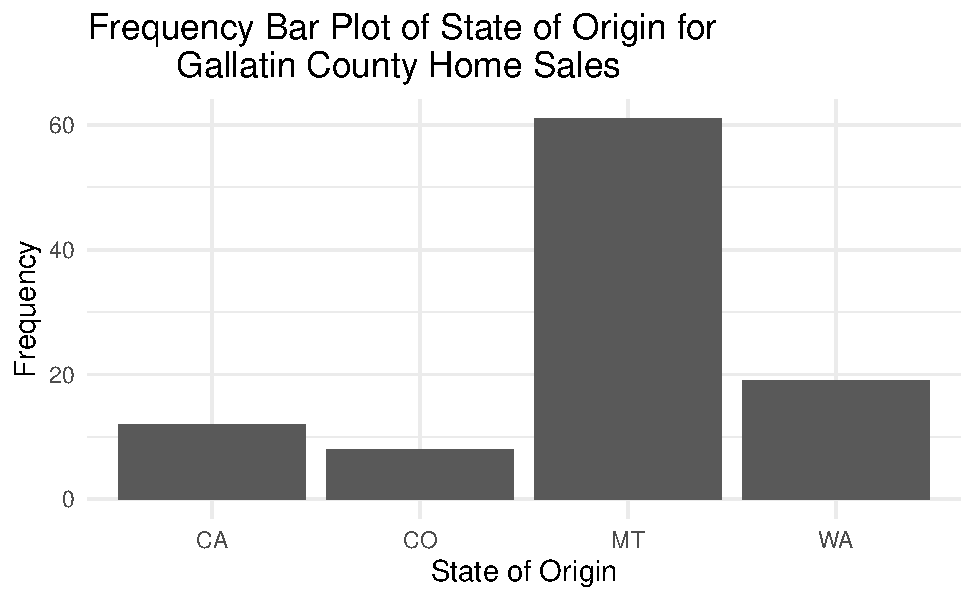
\includegraphics[width=0.65\linewidth]{03-LN03-EDA_files/figure-latex/unnamed-chunk-6-1} \end{center}

\begin{itemize}
\tightlist
\item
  What can we see from this plot?
\end{itemize}

\vspace{0.3in}

Additionally, we can create a relative frequency bar plot.

\begin{Shaded}
\begin{Highlighting}[]
\NormalTok{moving }\SpecialCharTok{\%\textgreater{}\%}
  \FunctionTok{ggplot}\NormalTok{(}\FunctionTok{aes}\NormalTok{(}\AttributeTok{x =}\NormalTok{ From))}\SpecialCharTok{+} \CommentTok{\#Enter the variable to plot}
  \FunctionTok{geom\_bar}\NormalTok{(}\FunctionTok{aes}\NormalTok{(}\AttributeTok{y =} \FunctionTok{after\_stat}\NormalTok{(prop), }\AttributeTok{group =} \DecValTok{1}\NormalTok{)) }\SpecialCharTok{+}
  \FunctionTok{labs}\NormalTok{(}\AttributeTok{title =} \StringTok{"Relative Frequency Bar Plot of State of Origin }
\StringTok{       for Gallatin County Home Sales"}\NormalTok{, }
       \CommentTok{\#Title your plot}
       \AttributeTok{y =} \StringTok{"Relative Frequency"}\NormalTok{, }\CommentTok{\#y{-}axis label}
       \AttributeTok{x =} \StringTok{"State of Origin"}\NormalTok{) }\CommentTok{\#x{-}axis label}
\end{Highlighting}
\end{Shaded}

\begin{center}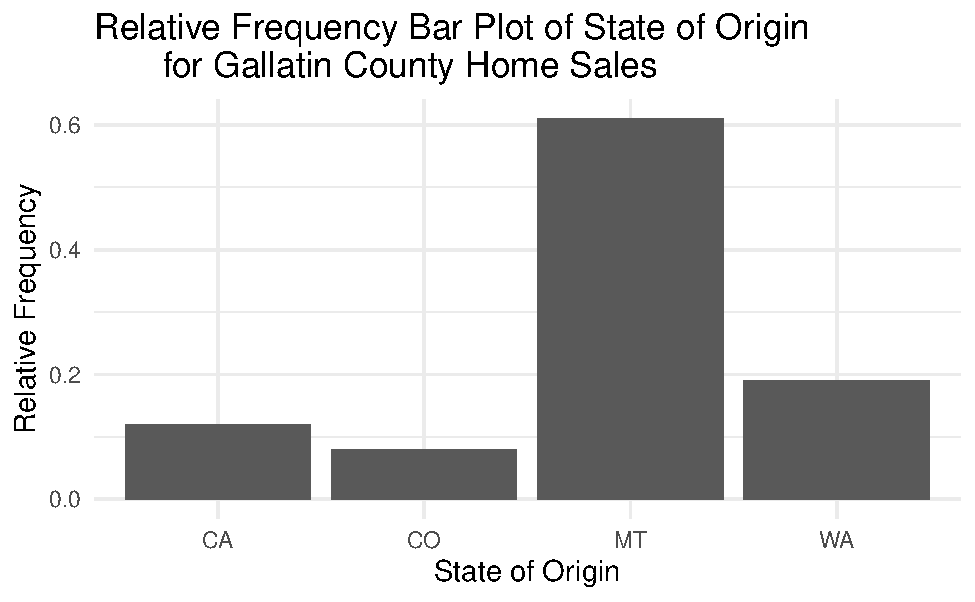
\includegraphics[width=0.65\linewidth]{03-LN03-EDA_files/figure-latex/unnamed-chunk-7-1} \end{center}

\setstretch{1.5}

\begin{itemize}
\tightlist
\item
  Note: the x-axis is the \_\_\_\_\_\_\_\_\_\_\_\_\_\_\_ between the frequency bar plot and the relative frequency bar plot. However, the \_\_\_\_\_\_\_\_\_\_\_\_\_\_ differs. The scale for the frequency bar plot goes from \_\_\_\_\_\_\_\_\_\_\_\_\_\_\_\_\_\_\_\_\_\_\_\_\_\_\_\_\_\_\_ and the scale for the relative frequency bar plot is from \_\_\_\_\_\_\_\_\_\_\_\_\_\_\_\_\_\_\_\_\_\_\_\_\_\_\_\_\_\_.
\end{itemize}

\setstretch{1}

\newpage

In a segmented bar plot, the bar for each category will sum to 1. In this first plot, we are plotting the row proportions calculated conditional on the age group.

\begin{Shaded}
\begin{Highlighting}[]
\NormalTok{moving }\SpecialCharTok{\%\textgreater{}\%}
  \FunctionTok{ggplot}\NormalTok{(}\FunctionTok{aes}\NormalTok{(}\AttributeTok{x =}\NormalTok{ Age\_Group, }\AttributeTok{fill =}\NormalTok{ From))}\SpecialCharTok{+} \CommentTok{\#Enter the variables to plot}
  \FunctionTok{geom\_bar}\NormalTok{(}\AttributeTok{stat =} \StringTok{"count"}\NormalTok{, }\AttributeTok{position =} \StringTok{"fill"}\NormalTok{) }\SpecialCharTok{+}
  \FunctionTok{labs}\NormalTok{(}\AttributeTok{title =} \StringTok{"Segmented bar plot of Age Group of Buyers by State of }
\StringTok{       Origin for Gallatin County Home Sales"}\NormalTok{, }
       \CommentTok{\#Title your plot}
       \AttributeTok{y =} \StringTok{"Relative Frequency"}\NormalTok{, }\CommentTok{\#y{-}axis label}
       \AttributeTok{x =} \StringTok{"Age Group"}\NormalTok{) }\SpecialCharTok{+} \CommentTok{\#x{-}axis label}
  \FunctionTok{scale\_fill\_grey}\NormalTok{()}
\end{Highlighting}
\end{Shaded}

\begin{center}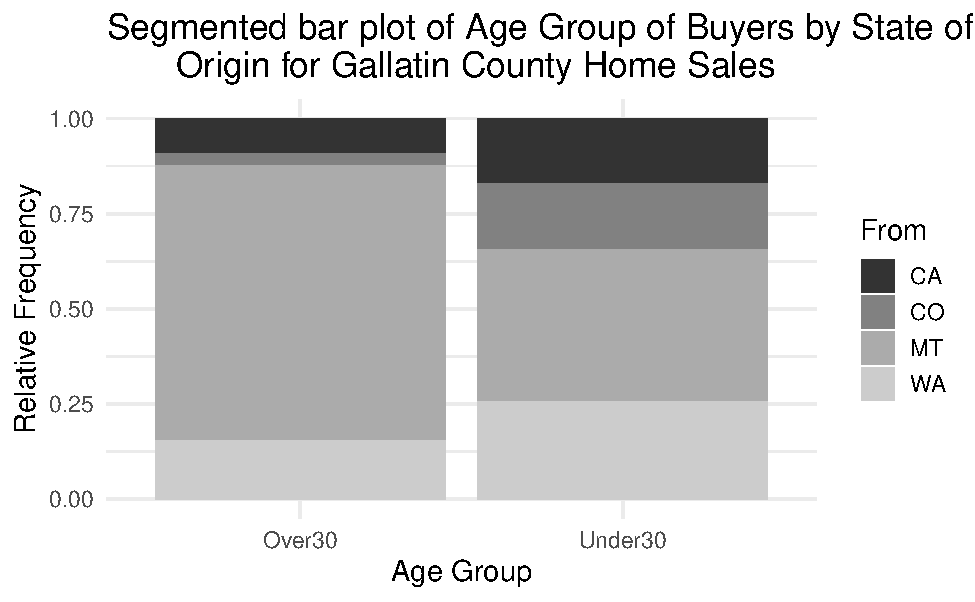
\includegraphics[width=0.55\linewidth]{03-LN03-EDA_files/figure-latex/unnamed-chunk-8-1} \end{center}

In this second plot, we are plotting the column proportions calculated conditional on the state of origin for the buyer.

\begin{Shaded}
\begin{Highlighting}[]
\NormalTok{moving }\SpecialCharTok{\%\textgreater{}\%}
  \FunctionTok{ggplot}\NormalTok{(}\FunctionTok{aes}\NormalTok{(}\AttributeTok{x =}\NormalTok{ From , }\AttributeTok{fill =}\NormalTok{ Age\_Group))}\SpecialCharTok{+} \CommentTok{\#Enter variables to plot}
  \FunctionTok{geom\_bar}\NormalTok{(}\AttributeTok{stat =} \StringTok{"count"}\NormalTok{, }\AttributeTok{position =} \StringTok{"fill"}\NormalTok{) }\SpecialCharTok{+}
  \FunctionTok{labs}\NormalTok{(}\AttributeTok{title =} \StringTok{"Segmented bar plot of State of Origin of Buyers by Age }
\StringTok{       Group for Gallatin County Home Sales"}\NormalTok{, }
       \CommentTok{\#Title your plot}
       \AttributeTok{y =} \StringTok{"Relative Frequency"}\NormalTok{, }\CommentTok{\#y{-}axis label}
       \AttributeTok{x =} \StringTok{"State of Origin"}\NormalTok{) }\SpecialCharTok{+} \CommentTok{\#x{-}axis label}
  \FunctionTok{scale\_fill\_grey}\NormalTok{()}
\end{Highlighting}
\end{Shaded}

\begin{center}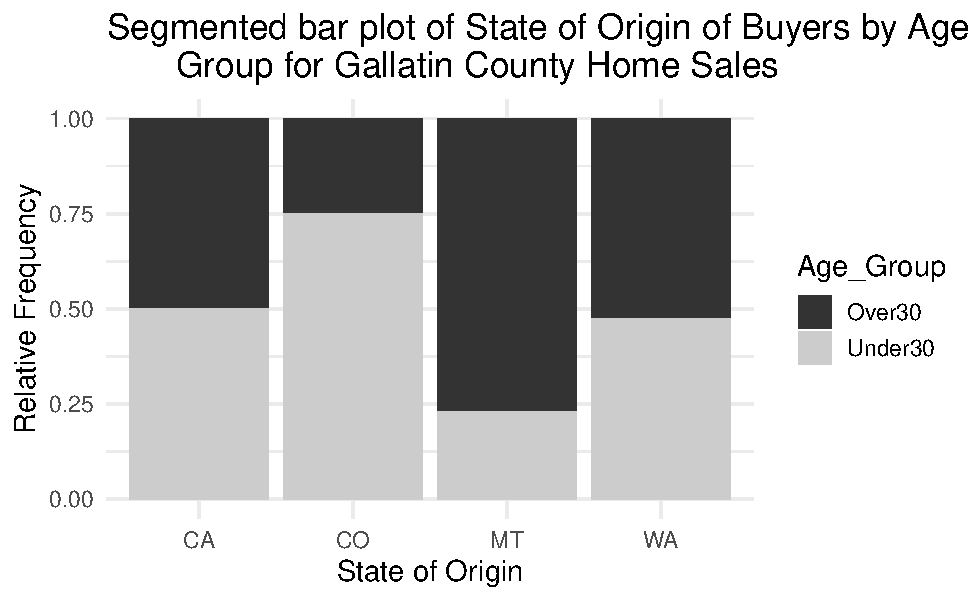
\includegraphics[width=0.55\linewidth]{03-LN03-EDA_files/figure-latex/unnamed-chunk-9-1} \end{center}

Mosaic plot:

\begin{Shaded}
\begin{Highlighting}[]
\NormalTok{moving}\SpecialCharTok{$}\NormalTok{Age\_Group }\OtherTok{\textless{}{-}} \FunctionTok{factor}\NormalTok{(moving}\SpecialCharTok{$}\NormalTok{Age\_Group, }\AttributeTok{levels =} \FunctionTok{c}\NormalTok{(}\StringTok{"Under30"}\NormalTok{, }\StringTok{"Over30"}\NormalTok{))}
\NormalTok{moving }\SpecialCharTok{\%\textgreater{}\%} \CommentTok{\# Data set piped into...}
  \FunctionTok{ggplot}\NormalTok{() }\SpecialCharTok{+}   \CommentTok{\# This specifies the variables}
  \FunctionTok{geom\_mosaic}\NormalTok{(}\FunctionTok{aes}\NormalTok{(}\AttributeTok{x=}\FunctionTok{product}\NormalTok{(From), }\AttributeTok{fill =}\NormalTok{ Age\_Group)) }\SpecialCharTok{+}  
    \CommentTok{\# Tell it to make a mosaic plot}
  \FunctionTok{labs}\NormalTok{(}\AttributeTok{title =} \StringTok{"Mosaic plot of State of Origin Segmented by }
\StringTok{  Age Group for Gallatin County Home Sales"}\NormalTok{,  }
       \CommentTok{\# Title your plot }
       \AttributeTok{x =} \StringTok{"State of Origin"}\NormalTok{,   }\CommentTok{\# Label the x axis}
       \AttributeTok{y =} \StringTok{""}\NormalTok{) }\SpecialCharTok{+}  \CommentTok{\# Remove y axis label}
    \FunctionTok{scale\_fill\_grey}\NormalTok{(}\AttributeTok{guide =} \FunctionTok{guide\_legend}\NormalTok{(}\AttributeTok{reverse =} \ConstantTok{TRUE}\NormalTok{)) }\CommentTok{\# Make figure color}
\end{Highlighting}
\end{Shaded}

\begin{center}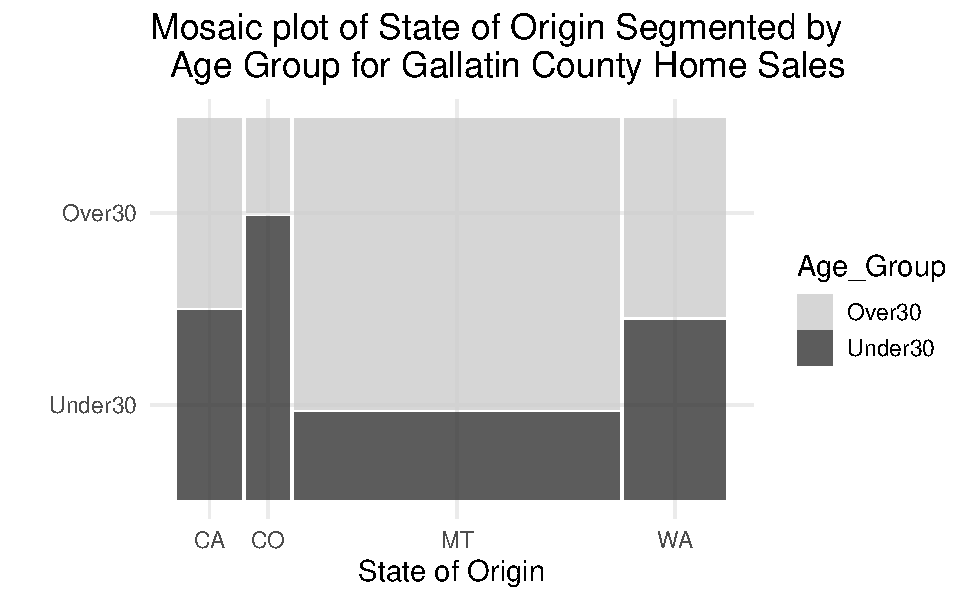
\includegraphics[width=0.75\linewidth]{03-LN03-EDA_files/figure-latex/unnamed-chunk-10-1} \end{center}

\begin{itemize}
\tightlist
\item
  Why is the bar for MT the widest on the mosaic plot?
\end{itemize}

\vspace{0.2in}

\newpage

\hypertarget{simpsons-paradox}{%
\subsubsection*{Simpson's paradox}\label{simpsons-paradox}}
\addcontentsline{toc}{subsubsection}{Simpson's paradox}

\setstretch{1.5}

\begin{itemize}
\tightlist
\item
  When an apparent \_\_\_\_\_\_\_\_\_\_\_\_\_ between explanatory and response variables reverses when accounting for \_\_\_\_\_\_\_\_\_\_\_\_\_\_ variable.
\end{itemize}

\setstretch{1}

Example: The ``Berkeley Dataset'' contains all 12,763 applicants to UC-Berkeley's graduate programs in Fall 1973. This dataset was published by UC Berkeley researchers in an analysis to understand the possible gender bias in admissions and has now become a classic example of Simpson's Paradox.

\begin{Shaded}
\begin{Highlighting}[]
\NormalTok{discrim }\OtherTok{\textless{}{-}} \FunctionTok{read.csv}\NormalTok{ (}\StringTok{"https://waf.cs.illinois.edu/discovery/berkeley.csv"}\NormalTok{)}

\NormalTok{discrim }\SpecialCharTok{\%\textgreater{}\%}
  \FunctionTok{ggplot}\NormalTok{(}\FunctionTok{aes}\NormalTok{(}\AttributeTok{x =}\NormalTok{Gender, }\AttributeTok{fill =}\NormalTok{ Admission))}\SpecialCharTok{+}
  \FunctionTok{geom\_bar}\NormalTok{(}\AttributeTok{stat =} \StringTok{"count"}\NormalTok{, }\AttributeTok{position =} \StringTok{"fill"}\NormalTok{) }\SpecialCharTok{+}
  \FunctionTok{labs}\NormalTok{(}\AttributeTok{title =} \StringTok{"Segmented bar plot of Sex of Berkley Applicants by }
\StringTok{       Admission Status"}\NormalTok{,}
       \AttributeTok{y =} \StringTok{"Relative Frequency"}\NormalTok{,}
       \AttributeTok{x =} \StringTok{"Sex"}\NormalTok{) }\SpecialCharTok{+}
  \FunctionTok{scale\_fill\_grey}\NormalTok{()}
\end{Highlighting}
\end{Shaded}

\begin{center}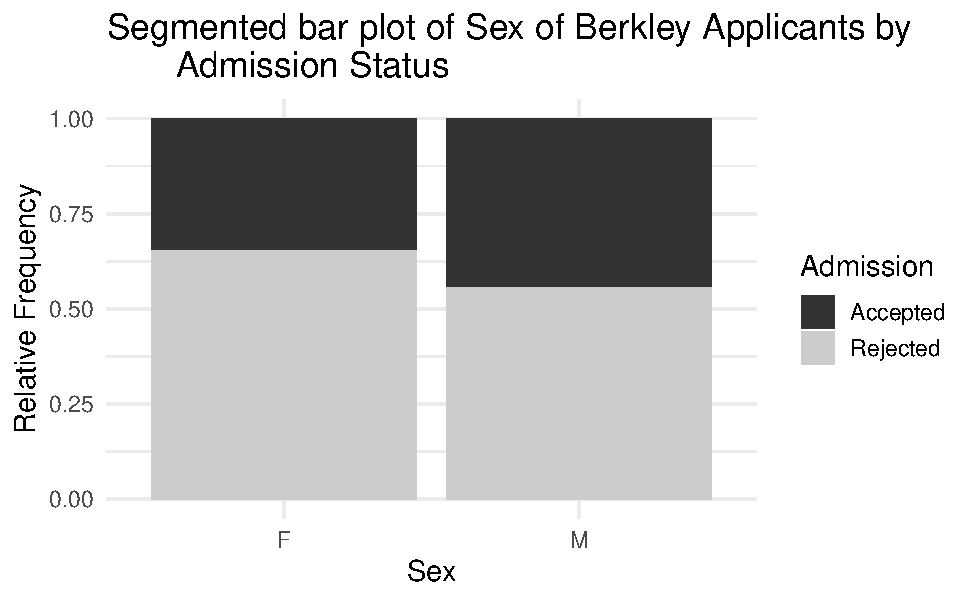
\includegraphics[width=0.85\linewidth]{03-LN03-EDA_files/figure-latex/unnamed-chunk-11-1} \end{center}

The data showed that 44\% of male applicants were accepted and 35\% of female applicants were accepted. Does it appear that the female students are discriminated against?

\vspace{0.1in}

We can break down the data by major. A major code (either A, B, C, D, E, F, or Other) was used.

\newpage

Here we look at the relationship between admission status and sex for Program A and for Program B.

\begin{center}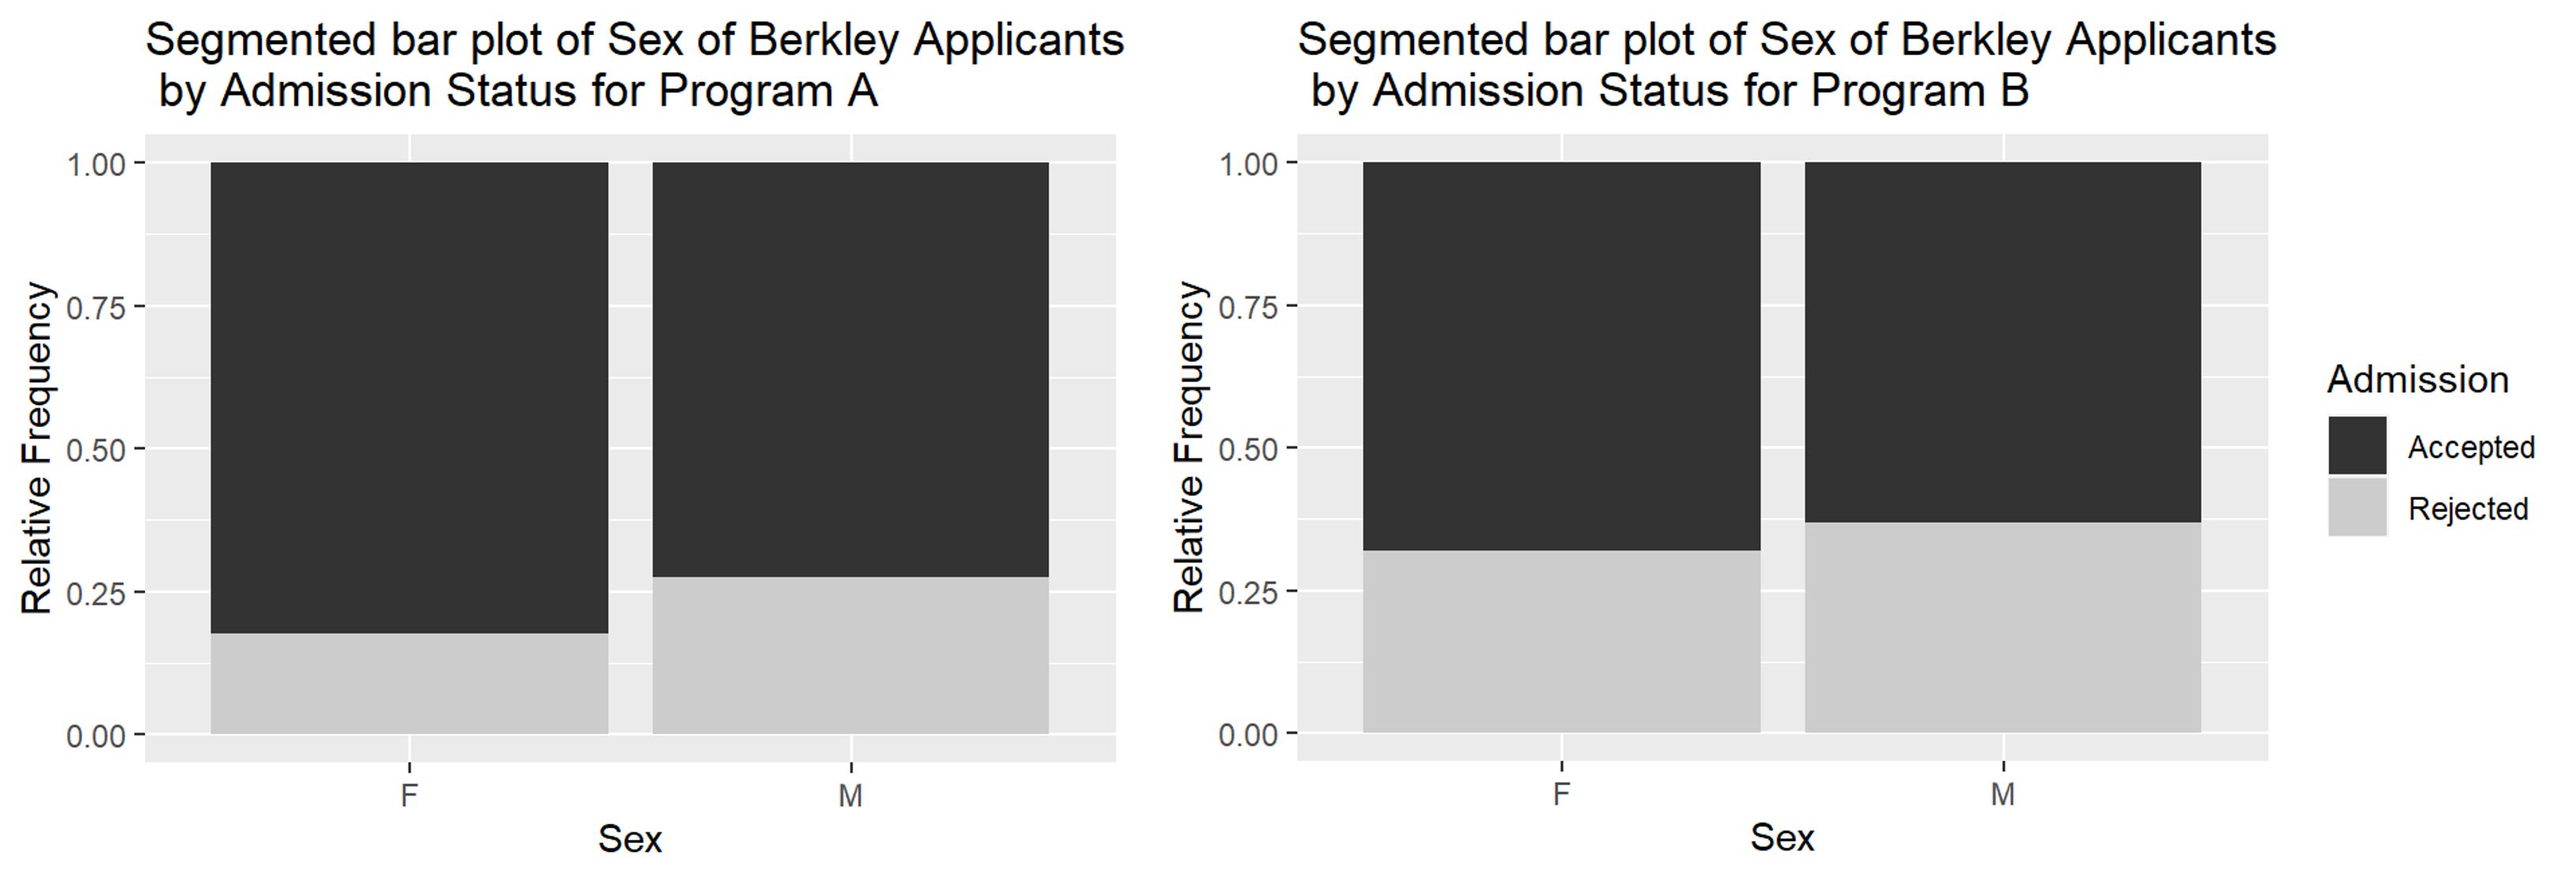
\includegraphics[width=0.85\linewidth]{images/SimPara_AB} \end{center}

Showing Program C and Program D.

\begin{center}\includegraphics[width=0.85\linewidth]{images/SimPara_cD} \end{center}

And finally, Program E and F.

\begin{center}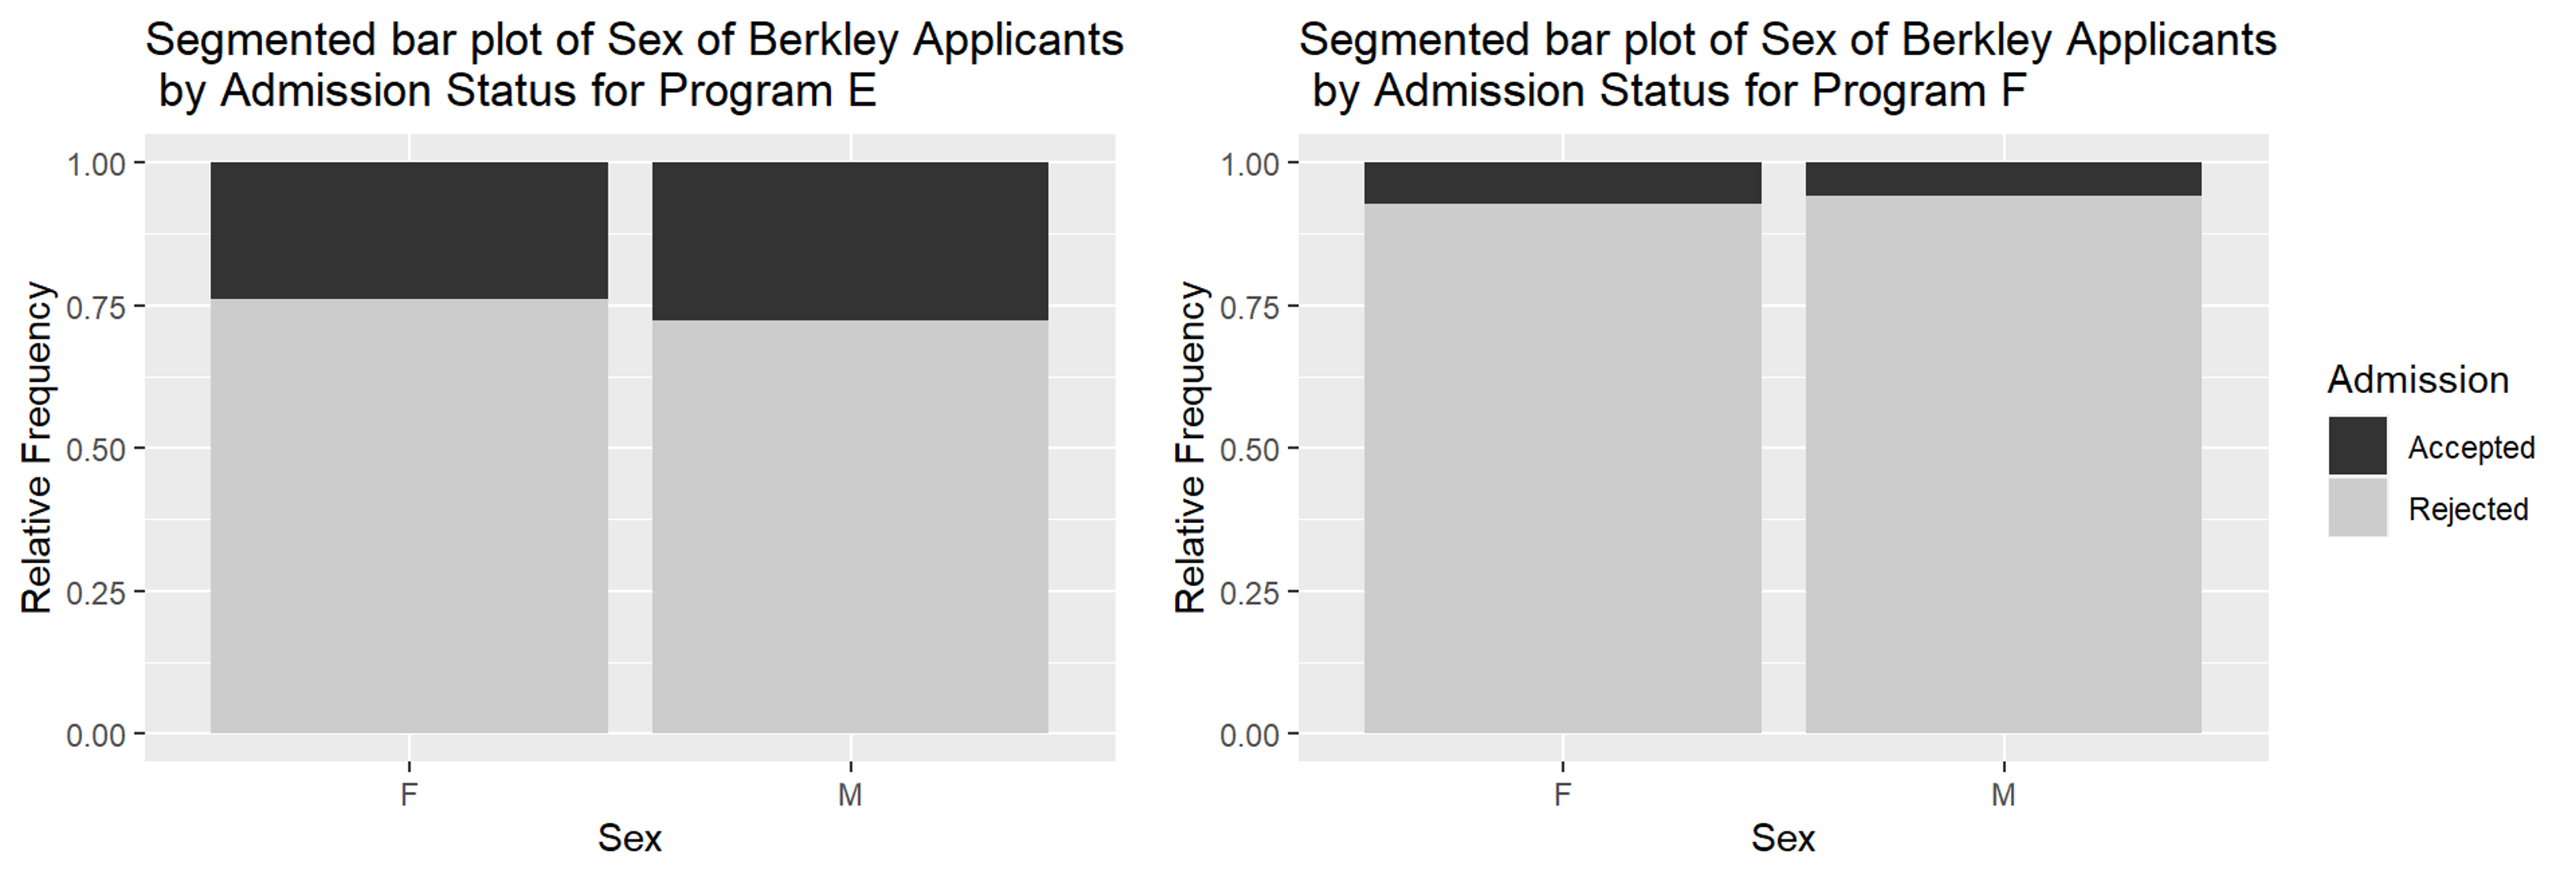
\includegraphics[width=0.85\linewidth]{images/SimPara_EF} \end{center}

We can see in several programs the acceptance rate is higher for females than for males.

\vspace{1in}

\newpage

\hypertarget{summarizing-quantitative-data}{%
\subsection*{Summarizing quantitative data}\label{summarizing-quantitative-data}}
\addcontentsline{toc}{subsection}{Summarizing quantitative data}

\setstretch{1.5}

Quantitative data can be numerically summarized by finding:

Two measures of center:

\begin{itemize}
\item
  Mean: \_\_\_\_\_\_\_\_\_\_\_\_ of all the \_\_\_\_\_\_\_\_\_\_\_\_\_ in the data set.

  \begin{itemize}
  \tightlist
  \item
    Sum the values in the data set and divide
    the sum by the sample size
  \end{itemize}
\item
  Notation used for the population mean:

  \begin{itemize}
  \tightlist
  \item
    Single quantitative variable:
  \end{itemize}
\end{itemize}

\vspace{0.2in}

\rgi \rgi - One categorical and one quantitative variable:

\vspace{0.2in}

\rgi \rgi \rgi - Subscripts represent the \_\_\_\_\_\_\_\_\_\_\_ variable groups

\begin{itemize}
\tightlist
\item
  Notation used for the sample mean:
\end{itemize}

\rgi \rgi - Single quantitative variable:

\vspace{0.2in}

\rgi \rgi - One categorical and one quantitative variable:

\vspace{0.2in}

\begin{itemize}
\item
  Median: Value at the \_\_\_\_\_\_\_\_\_\_\_\_\_ percentile

  \begin{itemize}
  \item
    \_\_\_\_\_\_\_\_\_\_ \% of values are at and \_\_\_\_\_\_\_\_\_\_\_ and at and \_\_\_\_\_\_\_\_\_\_\_ the value of the \_\_\_\_\_\_\_\_\_\_\_\_\_\_.
  \item
    Middle value in a list of ordered values
  \end{itemize}
\end{itemize}

Two measures of spread:

\begin{itemize}
\tightlist
\item
  Standard deviation: On average \_\_\_\_\_\_\_\_\_\_\_\_\_\_\_\_\_\_\_ each data point if from the \_\_\_\_\_\_\_\_\_\_\_\_\_\_ of the data set.
\end{itemize}

\vspace{1mm}

\rgi \rgi - Notation used for the population standard deviation

\vspace{0.2in}

\rgi \rgi - Notation used for the sample standard deviation

\vspace{0.2in}

\newpage

\begin{itemize}
\tightlist
\item
  Interquartile range: middle 50\% of data values
\end{itemize}

\rgi Formula:

\rgi \rgi Quartile 3 (Q3) - value at the 75th percentile

\rgi \rgi - \_\_\_\_\_\_\_\_\_\_\_\_ \% of values are at and \_\_\_\_\_\_\_\_\_\_\_\_\_ the value of Q3

\rgi \rgi Quartile 1 (Q1) - value at the 25th percentile

\rgi \rgi - \_\_\_\_\_\_\_\_\_\_\_\_\_ \% of values are at and \_\_\_\_\_\_\_\_\_\_\_\_\_ the value of Q1

\vspace{1mm}

\setstretch{1}

\hypertarget{types-of-plots}{%
\subsubsection*{Types of plots}\label{types-of-plots}}
\addcontentsline{toc}{subsubsection}{Types of plots}

We will revisit the moving to Montana data set and plot the age of the buyers.

\begin{itemize}
\tightlist
\item
  Dotplot:
\end{itemize}

\vspace{0.5in}

\begin{Shaded}
\begin{Highlighting}[]
\NormalTok{moving }\SpecialCharTok{\%\textgreater{}\%}
  \FunctionTok{ggplot}\NormalTok{(}\FunctionTok{aes}\NormalTok{(}\AttributeTok{x =}\NormalTok{ Age))}\SpecialCharTok{+} \CommentTok{\#Enter variable to plot}
  \FunctionTok{geom\_dotplot}\NormalTok{() }\SpecialCharTok{+} 
  \FunctionTok{labs}\NormalTok{(}\AttributeTok{title =} \StringTok{"Dotplot of Age of Buyers from Gallatin }
\StringTok{       County Home Sales"}\NormalTok{, }\CommentTok{\#Title your plot}
       \AttributeTok{x =} \StringTok{"Age"}\NormalTok{, }\CommentTok{\#x{-}axis label}
       \AttributeTok{y =} \StringTok{"Proportion"}\NormalTok{) }\CommentTok{\#y{-}axis label}
\end{Highlighting}
\end{Shaded}

\begin{center}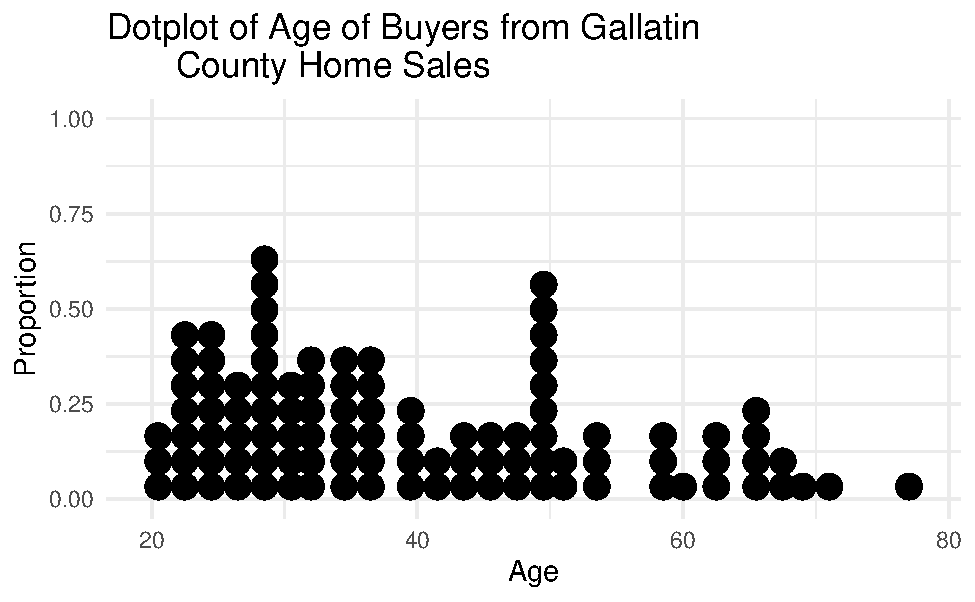
\includegraphics[width=0.75\linewidth]{03-LN03-EDA_files/figure-latex/unnamed-chunk-15-1} \end{center}

\newpage

\begin{itemize}
\tightlist
\item
  Histogram
\end{itemize}

\vspace{0.2in}

\begin{Shaded}
\begin{Highlighting}[]
\NormalTok{moving }\SpecialCharTok{\%\textgreater{}\%}
  \FunctionTok{ggplot}\NormalTok{(}\FunctionTok{aes}\NormalTok{(}\AttributeTok{x =}\NormalTok{ Age))}\SpecialCharTok{+}
  \FunctionTok{geom\_histogram}\NormalTok{(}\AttributeTok{binwidth =} \DecValTok{7}\NormalTok{) }\SpecialCharTok{+} 
  \FunctionTok{labs}\NormalTok{(}\AttributeTok{title =} \StringTok{"Histogram of Age of Buyers from Gallatin }
\StringTok{       County Home Sales"}\NormalTok{,}
       \CommentTok{\#Title your plot}
       \AttributeTok{x =} \StringTok{"Age"}\NormalTok{,}
       \AttributeTok{y =} \StringTok{"Count"}\NormalTok{)}
\end{Highlighting}
\end{Shaded}

\begin{center}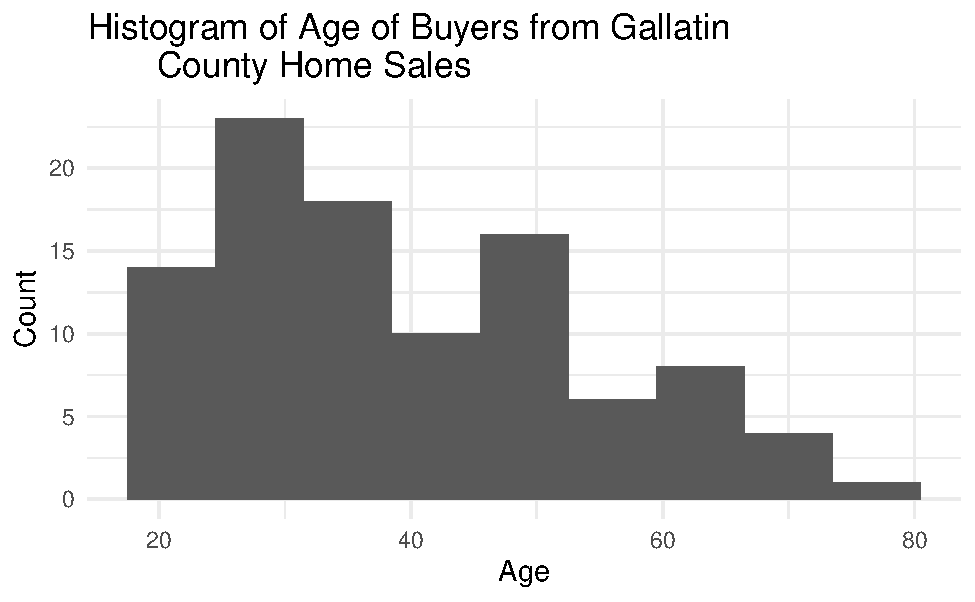
\includegraphics[width=0.7\linewidth]{03-LN03-EDA_files/figure-latex/unnamed-chunk-16-1} \end{center}

\newpage

\begin{itemize}
\item
  Boxplot

  \begin{itemize}
  \tightlist
  \item
    Five number summary: minimum, Q1, median, Q3, maximum
  \end{itemize}
\end{itemize}

\vspace{0.3in}

\begin{Shaded}
\begin{Highlighting}[]
\NormalTok{moving }\SpecialCharTok{\%\textgreater{}\%}
  \FunctionTok{ggplot}\NormalTok{(}\FunctionTok{aes}\NormalTok{(}\AttributeTok{x =}\NormalTok{ Age))}\SpecialCharTok{+} \CommentTok{\#Enter variable to plot}
  \FunctionTok{geom\_boxplot}\NormalTok{() }\SpecialCharTok{+} 
  \FunctionTok{labs}\NormalTok{(}\AttributeTok{title =} \StringTok{"Boxplot of Age of Buyers from Gallatin }
\StringTok{       County Home Sales"}\NormalTok{, }\CommentTok{\#Title your plot}
       \AttributeTok{x =} \StringTok{"Age"}\NormalTok{, }\CommentTok{\#x{-}axis label}
       \AttributeTok{y =} \StringTok{""}\NormalTok{) }\CommentTok{\#y{-}axis label}
\end{Highlighting}
\end{Shaded}

\begin{center}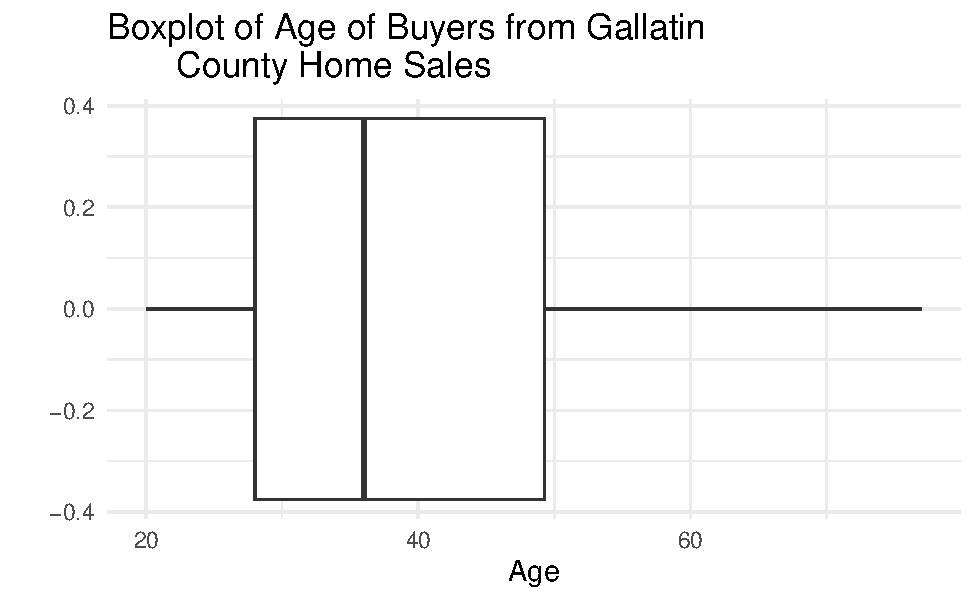
\includegraphics[width=0.7\linewidth]{03-LN03-EDA_files/figure-latex/unnamed-chunk-17-1} \end{center}

\begin{Shaded}
\begin{Highlighting}[]
\FunctionTok{favstats}\NormalTok{(moving}\SpecialCharTok{$}\NormalTok{Age)}
\CommentTok{\#\textgreater{}  min Q1 median    Q3 max  mean       sd   n missing}
\CommentTok{\#\textgreater{}   20 28     36 49.25  77 39.77 14.35471 100       0}
\end{Highlighting}
\end{Shaded}

Interpret the value of \(Q_3\) for the age of buyers.

\vspace{0.5in}

Interpret the value of s for the age of buyers.

\vspace{0.5in}

\newpage

\hypertarget{four-characteristics-of-plots-for-quantitative-variables}{%
\subsubsection*{Four characteristics of plots for quantitative variables}\label{four-characteristics-of-plots-for-quantitative-variables}}
\addcontentsline{toc}{subsubsection}{Four characteristics of plots for quantitative variables}

\begin{itemize}
\tightlist
\item
  Shape: overall pattern of the data
\end{itemize}

\begin{center}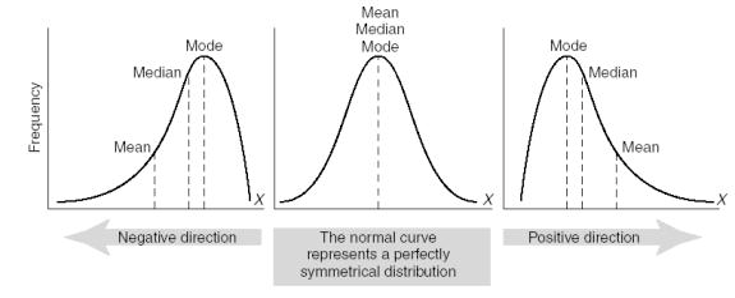
\includegraphics[width=0.8\linewidth]{images/shape} \end{center}

\rgi \rgi - What is the shape of the distribution of age of buyers for Gallatin County home sales?

\vspace{0.3in}

\begin{itemize}
\tightlist
\item
  Center:
\end{itemize}

\rgi Mean or Median

\rgi \rgi - Report the measure of center for the boxplot of age of buyers for Gallatin County home sales.

\vspace{0.3in}

\begin{itemize}
\tightlist
\item
  Spread (or variability):
\end{itemize}

\rgi Standard deviation or IQR

\rgi \rgi - Report the IQR for the distribution of age of buyers from Gallatin County home sales.

\vspace{0.3in}

\begin{itemize}
\tightlist
\item
  Outliers?
\end{itemize}

\rgi values \textless{} \(Q_1 - 1.5 \times IQR\)

\rgi values \textgreater{} \(Q_3 + 1.5 \times IQR\)

\rgi \rgi - Use these formulas to show that there are no outliers in the distribution of age of buyers from Gallatin County home sales.

\vspace{0.8in}
\newpage

Let's look at side-by-side boxplot of the variable age by state of origin moved from.

\begin{Shaded}
\begin{Highlighting}[]
\NormalTok{moving }\SpecialCharTok{\%\textgreater{}\%}  \CommentTok{\# Data set piped into...}
  \FunctionTok{ggplot}\NormalTok{(}\FunctionTok{aes}\NormalTok{(}\AttributeTok{y =}\NormalTok{ Age, }\AttributeTok{x =}\NormalTok{ From))}\SpecialCharTok{+}  \CommentTok{\# Identify variables}
  \FunctionTok{geom\_boxplot}\NormalTok{()}\SpecialCharTok{+}  \CommentTok{\# Tell it to make a box plot}
  \FunctionTok{labs}\NormalTok{(}\AttributeTok{title =} \StringTok{"Side by side box plot of Age by State of Origin }
\StringTok{  of Buyers from Gallatin County Home Sales"}\NormalTok{,  }\CommentTok{\# Title}
       \AttributeTok{x =} \StringTok{"State of Origin"}\NormalTok{,    }\CommentTok{\# x{-}axis label}
       \AttributeTok{y =} \StringTok{"Age"}\NormalTok{)  }\CommentTok{\# y{-}axis label}
\end{Highlighting}
\end{Shaded}

\begin{center}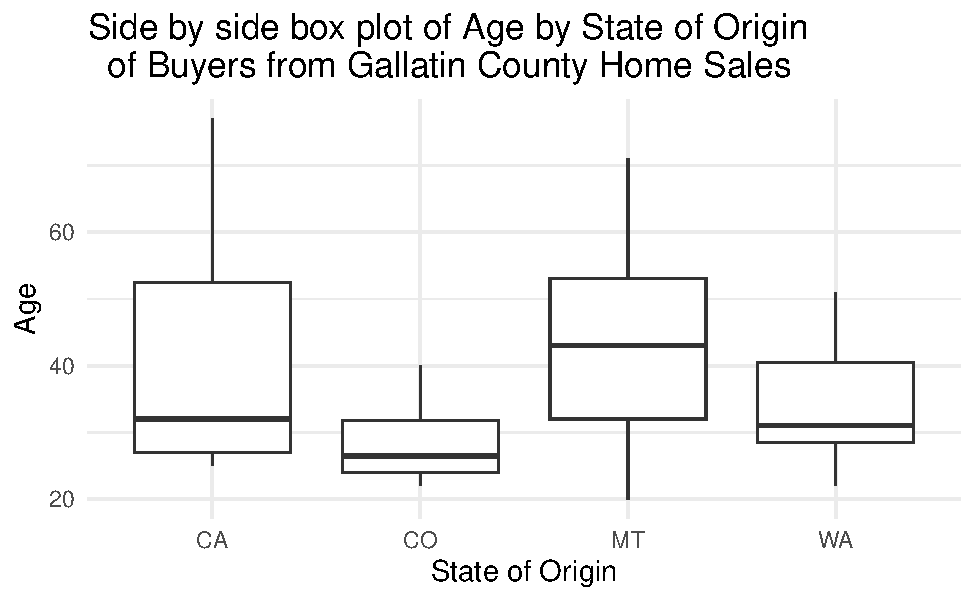
\includegraphics[width=0.85\linewidth]{03-LN03-EDA_files/figure-latex/unnamed-chunk-20-1} \end{center}

\begin{itemize}
\tightlist
\item
  Which state of origin had the oldest median age of buyers from sampled home sales?
\end{itemize}

\vspace{0.3in}

\begin{itemize}
\tightlist
\item
  Which state of origin had the most variability in age of buyers from sampled home sales?
\end{itemize}

\vspace{0.3in}

\begin{itemize}
\tightlist
\item
  Which state of origin had the most symmetric distribution of ages of buyers from sampled home sales?
\end{itemize}

\vspace{0.3in}

\begin{itemize}
\tightlist
\item
  Which state of origin had outliers for the age of buyers from sampled home sales?
\end{itemize}

\vspace{0.3in}

\newpage

\hypertarget{robust-statistics}{%
\subsubsection*{Robust statistics}\label{robust-statistics}}
\addcontentsline{toc}{subsubsection}{Robust statistics}

Let's review the summary statistics and histogram of age of buyers from sampled home sales.

\begin{center}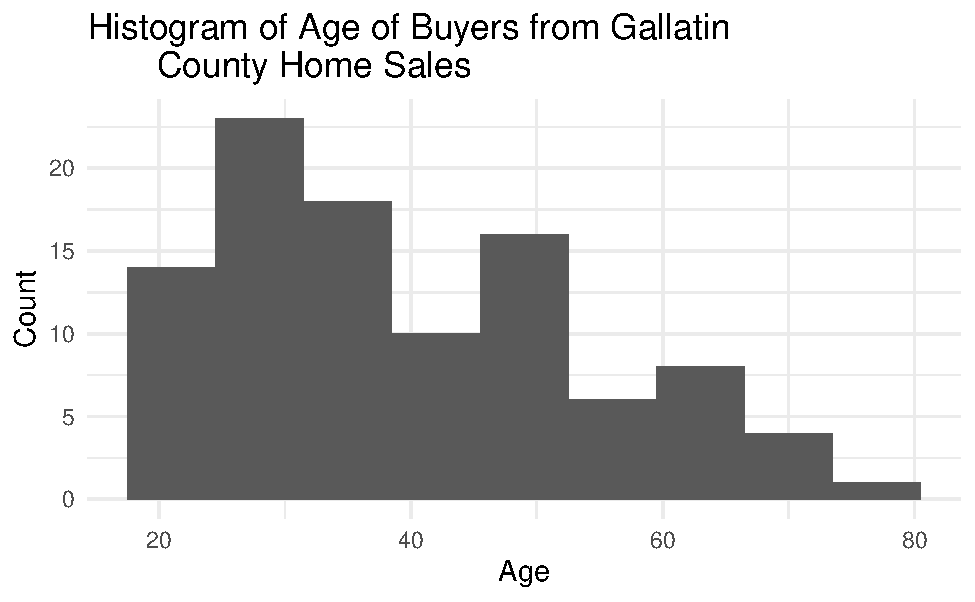
\includegraphics[width=0.85\linewidth]{03-LN03-EDA_files/figure-latex/unnamed-chunk-21-1} \end{center}

\begin{verbatim}
#>  min Q1 median    Q3 max  mean       sd   n missing
#>   20 28     36 49.25  77 39.77 14.35471 100       0
\end{verbatim}

\setstretch{1.5}

Notice that the \_\_\_\_\_\_\_\_\_\_\_\_\_ has been pulled in the direction of the \_\_\_\_\_\_\_\_\_\_\_\_\_\_\_.

\begin{itemize}
\item
  The \_\_\_\_\_\_\_\_\_\_\_ is a \_\_\_\_\_\_\_\_\_\_\_\_\_\_ measure of center.
\item
  The \_\_\_\_\_\_\_\_\_\_\_ is a \_\_\_\_\_\_\_\_\_\_\_\_\_\_ measure of spread.
\item
  Robust means not \_\_\_\_\_\_\_\_\_\_\_\_\_\_\_\_\_ by.
\end{itemize}

When the distribution is symmetric use the \_\_\_\_\_\_\_\_\_\_\_\_ as the measure of center and the \_\_\_\_\_\_\_\_\_\_\_ as the measure of spread.

When the distribution is skewed with outliers use the \_\_\_\_\_\_\_\_\_\_\_\_\_ as the measure of center and the \_\_\_\_\_\_\_\_\_\_\_\_ as the measure of spread.

\setstretch{1}

\newpage

\hypertarget{out-of-class-activity-week-3-summarizing-categorical-variables}{%
\section{Out-of-Class Activity Week 3: Summarizing Categorical Variables}\label{out-of-class-activity-week-3-summarizing-categorical-variables}}

\setstretch{1}

\hypertarget{learning-outcomes-4}{%
\subsection{Learning outcomes}\label{learning-outcomes-4}}

\begin{itemize}
\item
  Identify and create appropriate summary statistics and plots given a data set or research question involving categorical variables.
\item
  Plots for a single categorical variable: bar plot.
\item
  Plots for association between two categorical variables:
  segmented bar plot, mosaic plot.
\end{itemize}

\hypertarget{terminology-review-4}{%
\subsection{Terminology review}\label{terminology-review-4}}

In today's activity, we will review summary measures and plots for categorical variables. Some terms covered in this activity are:

\begin{itemize}
\item
  Proportions
\item
  Bar plots
\item
  Segmented bar plots
\item
  Mosaic plots
\end{itemize}

To review these concepts, see Chapter 4 in the textbook.

\hypertarget{graphing-categorical-variables}{%
\subsection{Graphing categorical variables}\label{graphing-categorical-variables}}

For this out-of-class activity we will walk through how to use the statistical package R to analyze data through the IDE (integrated development environment) RStudio. Even though the completed code is provided for you in this activity, we recommend that you login to the RStudio server and follow along to see how to create the plots and get the summary statistics for categorical data.

For almost all activities and labs it will be necessary to upload the provided R script file from D2L for that day. Follow these steps to upload the necessary R script file for this activity:

\begin{itemize}
\tightlist
\item
  Download the Myopia Activity R script file from D2L.
\item
  Click ``Upload'' in the ``Files'' tab in the bottom right window of RStudio. In the pop-up window, click ``Choose File'', and navigate to the folder where the Myopia Activity R script file is saved (most likely in your downloads folder). Click ``Open''; then click ``Ok''.
\item
  You should see the uploaded file appear in the list of files in the bottom right window. Click on the file name to open the file in the Editor window (upper left window).
\end{itemize}

Notice that the first three lines of code contain a prompt called, \texttt{library}. Packages needed to run functions in R are stored in directories called libraries. When using the MSU RStudio server, all the packages needed for the class are already installed. We simply must tell R which packages we need for each R script file. We use the prompt \texttt{library} to load each \textbf{package} (or library) needed for each activity. Note, these \texttt{library} lines MUST be run each time you open a R script file in order for the functions in R to work.

\begin{itemize}
\tightlist
\item
  Highlight and run lines 1--3 to load the packages needed for this activity. Notice the use of the \# symbol in the R script file. The \# sign is not part of the R code. It is used by these authors to add comments to the R code and explain what each call is telling the program to do.
  R will ignore everything after a \# sign when executing the code. Refer to the instructions following the \# sign to understand what you need to enter in the code.
\end{itemize}

\hypertarget{nightlight-use-and-myopia}{%
\subsection*{Nightlight use and myopia}\label{nightlight-use-and-myopia}}
\addcontentsline{toc}{subsection}{Nightlight use and myopia}

In a study reported in \emph{Nature} (Quinn et al. 1999), a survey of 479 children found that those who had slept with a nightlight or in a fully lit room before the age of two had a higher incidence of nearsightedness (myopia) later in childhood.

In this study, there are two variables studied: \texttt{Light}: level of light in room at night (no light, nightlight, full light) and \texttt{Sight}: level of myopia developed later in childhood (high myopia, myopia, no myopia).

\begin{enumerate}
\def\labelenumi{\arabic{enumi}.}
\tightlist
\item
  Which variable is the explanatory variable? Which is the response variable?
\end{enumerate}

\vspace{0.8in}

An important part of understanding data is to create visual pictures of what the data represent. In this activity, we will create graphical representations of categorical data.

\hypertarget{r-code}{%
\subsubsection*{R code}\label{r-code}}
\addcontentsline{toc}{subsubsection}{R code}

Throughout these activities, we will often include the R code you would use in order to produce output or plots. These ``code chunks'' appear in gray. In the code chunk below, we demonstrate how to read the data set into R using the \texttt{read.csv()} function. The line of code shown below (line 6 in the R script file) reads in the data set and names the data set \texttt{myopia}.

\begin{itemize}
\tightlist
\item
  Highlight and run line 6 in the R script file to load the data from the Stat 216 webpage.
\end{itemize}

\begin{Shaded}
\begin{Highlighting}[]
\CommentTok{\# This will read in the data set}
\NormalTok{myopia }\OtherTok{\textless{}{-}} \FunctionTok{read.csv}\NormalTok{(}\StringTok{"https://math.montana.edu/courses/s216/data/ChildrenLightSight.csv"}\NormalTok{) }
\end{Highlighting}
\end{Shaded}

\begin{itemize}
\tightlist
\item
  Click on the data set name (\texttt{myopia}) in the Environment tab (upper right window). This will open the data set in a 2nd tab in the Editor window (upper left window). R is case sensitive, which means that you must always type the name of a variable EXACTLY as it is written in the data set including upper and lower case letters and without misspellings!
\end{itemize}

There are two variables in this data set. \texttt{Light} with three possible outcomes: \texttt{Full\ Light}, \texttt{Nightlight}, and \texttt{No\ Light} and \texttt{Sight} with three possible outcomes: \texttt{High\ Myopia}, \texttt{Myopia}, and \texttt{No\ Myopia}.

\hypertarget{displaying-a-single-categorical-variable}{%
\subsubsection*{Displaying a single categorical variable}\label{displaying-a-single-categorical-variable}}
\addcontentsline{toc}{subsubsection}{Displaying a single categorical variable}

If we wanted to know how many children in our data set were in each level of myopia, we could create a frequency bar plot of the variable \texttt{Sight}.

\begin{itemize}
\item
  In the R code below (and the provided R script file), we will enter the variable name, \texttt{Sight} (\emph{note the capital S}), for \texttt{variable} into the \texttt{ggplot} code. This is in line 12 in the R script file.
\item
  Highlight and run lines 11--16 to create the plot. Note: this is a \textbf{frequency} bar plot plotting counts (the number of children in each level of sight is displayed on the \(y\)-axis).
\end{itemize}

\begin{Shaded}
\begin{Highlighting}[]
\NormalTok{myopia }\SpecialCharTok{\%\textgreater{}\%} \CommentTok{\# Data set piped into...}
\FunctionTok{ggplot}\NormalTok{(}\FunctionTok{aes}\NormalTok{(}\AttributeTok{x =}\NormalTok{ varible)) }\SpecialCharTok{+}   \CommentTok{\# This specifies the variable}
  \FunctionTok{geom\_bar}\NormalTok{(}\AttributeTok{stat =} \StringTok{"count"}\NormalTok{) }\SpecialCharTok{+}  \CommentTok{\# Tell it to make a bar plot}
  \FunctionTok{labs}\NormalTok{(}\AttributeTok{title =} \StringTok{"Frequency Bar Plot of Level of Myopia for Children"}\NormalTok{,  }
       \CommentTok{\# Give your plot a title}
       \AttributeTok{x =} \StringTok{"Level of Myopia"}\NormalTok{,   }\CommentTok{\# Label the x axis}
       \AttributeTok{y =} \StringTok{"Frequency"}\NormalTok{)  }\CommentTok{\# Label the y axis}
\end{Highlighting}
\end{Shaded}

\newpage

Frequency bar plot of sight:

\begin{Shaded}
\begin{Highlighting}[]
\NormalTok{myopia }\SpecialCharTok{\%\textgreater{}\%} \CommentTok{\# Data set piped into...}
\FunctionTok{ggplot}\NormalTok{(}\FunctionTok{aes}\NormalTok{(}\AttributeTok{x =}\NormalTok{ Sight)) }\SpecialCharTok{+}   \CommentTok{\# This specifies the variable}
  \FunctionTok{geom\_bar}\NormalTok{(}\AttributeTok{stat =} \StringTok{"count"}\NormalTok{) }\SpecialCharTok{+}  \CommentTok{\# Tell it to make a bar plot}
  \FunctionTok{labs}\NormalTok{(}\AttributeTok{title =} \StringTok{"Frequency Bar Plot of Level of Myopia for Children"}\NormalTok{,  }
       \CommentTok{\# Give your plot a title}
       \AttributeTok{x =} \StringTok{"Level of Myopia"}\NormalTok{,   }\CommentTok{\# Label the x axis}
       \AttributeTok{y =} \StringTok{"Frequency"}\NormalTok{)  }\CommentTok{\# Label the y axis}
\end{Highlighting}
\end{Shaded}

\begin{center}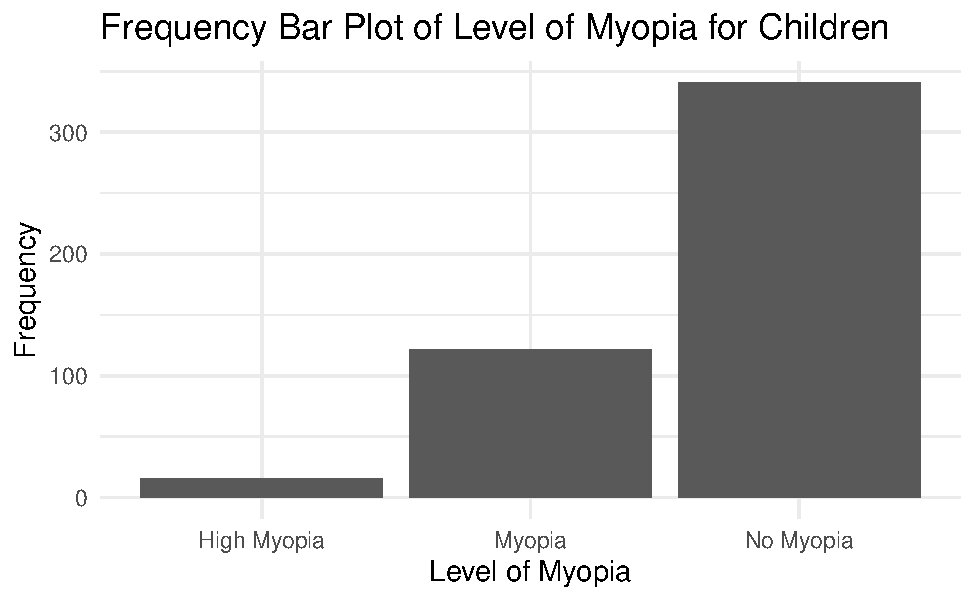
\includegraphics[width=0.5\linewidth]{03-OCA02-EDA_files/figure-latex/unnamed-chunk-3-1} \end{center}

\begin{enumerate}
\def\labelenumi{\arabic{enumi}.}
\setcounter{enumi}{1}
\tightlist
\item
  Using the bar chart created, estimate how many children have some level of myopia.
\end{enumerate}

\vspace{0.2in}

We could also choose to display the data as a proportion in a \textbf{relative frequency} bar plot. To find the relative frequency, the count in each level of myopia is divided by the sample size. This calculation is the sample proportion for each level of myopia. Notice that in this code we told R to create a bar plot with proportions.

\begin{Shaded}
\begin{Highlighting}[]
\NormalTok{myopia }\SpecialCharTok{\%\textgreater{}\%} \CommentTok{\# Data set piped into...}
\FunctionTok{ggplot}\NormalTok{(}\FunctionTok{aes}\NormalTok{(}\AttributeTok{x =}\NormalTok{ Sight)) }\SpecialCharTok{+}   \CommentTok{\# This specifies the variable}
  \FunctionTok{geom\_bar}\NormalTok{(}\FunctionTok{aes}\NormalTok{(}\AttributeTok{y =} \FunctionTok{after\_stat}\NormalTok{(prop), }\AttributeTok{group =} \DecValTok{1}\NormalTok{)) }\SpecialCharTok{+}  \CommentTok{\# Tell it to make a bar plot with proportions}
  \FunctionTok{labs}\NormalTok{(}\AttributeTok{title =} \StringTok{"Relative Frequency Bar Plot of Level of Myopia for Children"}\NormalTok{,  }\CommentTok{\# Give your plot a title}
       \AttributeTok{x =} \StringTok{"Level of Myopia"}\NormalTok{,   }\CommentTok{\# Label the x axis}
       \AttributeTok{y =} \StringTok{"Relative Frequency"}\NormalTok{)  }\CommentTok{\# Label the y axis}
\end{Highlighting}
\end{Shaded}

\begin{center}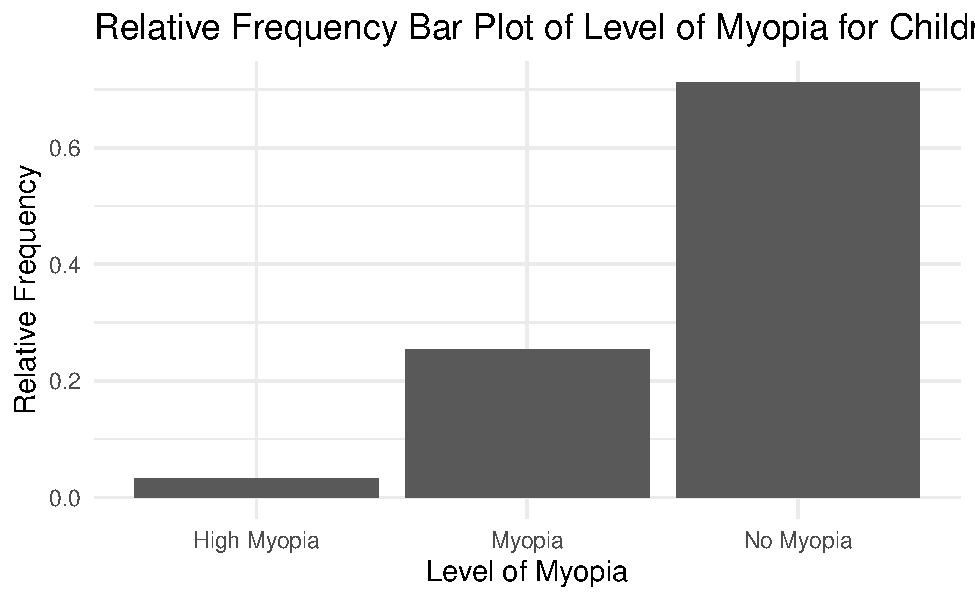
\includegraphics[width=0.5\linewidth]{03-OCA02-EDA_files/figure-latex/unnamed-chunk-4-1} \end{center}

\begin{enumerate}
\def\labelenumi{\arabic{enumi}.}
\setcounter{enumi}{2}
\tightlist
\item
  Which features in the relative frequency bar plot are the same as the frequency bar plot? Which are different?
\end{enumerate}

\vspace{0.3in}

\hypertarget{displaying-two-categorical-variables}{%
\subsubsection*{Displaying two categorical variables}\label{displaying-two-categorical-variables}}
\addcontentsline{toc}{subsubsection}{Displaying two categorical variables}

Is there an association between the level of light in a room and the development of myopia?

\begin{itemize}
\item
  Fill in the name of the explanatory variable, \texttt{Light} for explanatory and name of the response variable, \texttt{Sight} in line 29 in the R script file.
\item
  Highlight and run line 29 to get the counts for each combination of levels of variables.
\end{itemize}

\begin{Shaded}
\begin{Highlighting}[]
\NormalTok{myopia }\SpecialCharTok{\%\textgreater{}\%} \FunctionTok{group\_by}\NormalTok{(explanatory) }\SpecialCharTok{\%\textgreater{}\%} \FunctionTok{count}\NormalTok{(response)}
\end{Highlighting}
\end{Shaded}

Here is the completed code and R output:

\begin{Shaded}
\begin{Highlighting}[]
\NormalTok{myopia }\SpecialCharTok{\%\textgreater{}\%} \FunctionTok{group\_by}\NormalTok{(Light) }\SpecialCharTok{\%\textgreater{}\%} \FunctionTok{count}\NormalTok{(Sight) }\SpecialCharTok{\%\textgreater{}\%} \FunctionTok{print}\NormalTok{(}\AttributeTok{n=}\DecValTok{9}\NormalTok{)}
\CommentTok{\#\textgreater{} \# A tibble: 9 x 3}
\CommentTok{\#\textgreater{} \# Groups:   Light [3]}
\CommentTok{\#\textgreater{}   Light      Sight           n}
\CommentTok{\#\textgreater{}   \textless{}chr\textgreater{}      \textless{}chr\textgreater{}       \textless{}int\textgreater{}}
\CommentTok{\#\textgreater{} 1 Full Light High Myopia     5}
\CommentTok{\#\textgreater{} 2 Full Light Myopia         42}
\CommentTok{\#\textgreater{} 3 Full Light No Myopia      38}
\CommentTok{\#\textgreater{} 4 Nightlight High Myopia     9}
\CommentTok{\#\textgreater{} 5 Nightlight Myopia         65}
\CommentTok{\#\textgreater{} 6 Nightlight No Myopia     149}
\CommentTok{\#\textgreater{} 7 No Light   High Myopia     2}
\CommentTok{\#\textgreater{} 8 No Light   Myopia         15}
\CommentTok{\#\textgreater{} 9 No Light   No Myopia     154}
\end{Highlighting}
\end{Shaded}

\begin{enumerate}
\def\labelenumi{\arabic{enumi}.}
\setcounter{enumi}{3}
\tightlist
\item
  Fill in the following table with the values from the R output.
\end{enumerate}

\begin{center}
\begingroup
\setlength{\tabcolsep}{14pt} % Default value: 6pt
\renewcommand{\arraystretch}{2} % Default value: 1
\begin{tabular}{|c|c|c|c|c|}
\hline
 & \multicolumn{3}{|c|}{\textbf{Light Level}} & \\ \hline
\textbf{Myopia Level} & Full Light & Nightlight & No Light & Total \\ \hline
 High Myopia & & & & \\ \hline
 Myopia & & & & \\ \hline
 No Myopia & & & & \\ \hline
 Total & & & & \\ \hline  
\end{tabular}
\endgroup
\end{center}

In the following questions, use the table to calculate the described proportions. Notation is important for each calculation. Since this is sample data, it is appropriate to use statistic notation for the proportion, \(\hat{p}\). When calculating a proportion dependent on a single level of a variable, subscripts are needed when reporting the notation.

\begin{enumerate}
\def\labelenumi{\arabic{enumi}.}
\setcounter{enumi}{4}
\item
  Calculate the proportion of children with no myopia. Use appropriate notation.
  \vspace{0.3in}
\item
  Calculate the proportion of children with no myopia among those that slept with full light. Use appropriate notation.
  \vspace{0.3in}
\item
  Calculate the proportion of children with no myopia among those that slept with no light. Use appropriate notation.
  \vspace{0.3in}
\item
  Calculate the difference in proportion of children with no myopia for those that slept with full light minus those who slept with no light. Give the appropriate notation. Use full light minus no light as the order of subtraction.
  \vspace{0.4in}
\item
  Interpret the difference in proportion calculated in question 8 in context of the study.
\end{enumerate}

\vspace{0.5in}

Two types of plots can be created to display two categorical variables. To examine the differences in level of myopia for the level of light, we will first create a segmented bar plot of \texttt{Light} segmented by \texttt{Sight}.

\begin{itemize}
\item
  To create the segmented bar plot enter the variable name, \texttt{Light} for \texttt{explanatory} and the variable name, \texttt{Sight} for \texttt{response} in line 35 in the R script file.
\item
  Highlight and run lines 34--40.
\end{itemize}

\begin{Shaded}
\begin{Highlighting}[]
\NormalTok{myopia }\SpecialCharTok{\%\textgreater{}\%} \CommentTok{\# Data set piped into...}
\FunctionTok{ggplot}\NormalTok{(}\FunctionTok{aes}\NormalTok{(}\AttributeTok{x =}\NormalTok{ explanatory, }\AttributeTok{fill =}\NormalTok{ response)) }\SpecialCharTok{+}   \CommentTok{\# This specifies the variables}
  \FunctionTok{geom\_bar}\NormalTok{(}\AttributeTok{stat =} \StringTok{"count"}\NormalTok{, }\AttributeTok{position =} \StringTok{"fill"}\NormalTok{) }\SpecialCharTok{+}  \CommentTok{\# Tell it to make a stacked bar plot}
  \FunctionTok{labs}\NormalTok{(}\AttributeTok{title =} \StringTok{"Segmented Bar Plot of Night Light Use by Level of }
\StringTok{       Myopia for Children"}\NormalTok{,  }\CommentTok{\# Make sure to title your plot }
       \AttributeTok{x =} \StringTok{"Level of Light"}\NormalTok{,   }\CommentTok{\# x axis label}
       \AttributeTok{y =} \StringTok{"Relative Frequency"}\NormalTok{)  }\SpecialCharTok{+} \CommentTok{\# y axis label}
  \FunctionTok{scale\_fill\_viridis\_d}\NormalTok{()  }\CommentTok{\# Make figure color}
\end{Highlighting}
\end{Shaded}

Segmented bar plot of Night Light Use by Level of Myopia:

\begin{Shaded}
\begin{Highlighting}[]
\NormalTok{myopia }\SpecialCharTok{\%\textgreater{}\%} \CommentTok{\# Data set piped into...}
\FunctionTok{ggplot}\NormalTok{(}\FunctionTok{aes}\NormalTok{(}\AttributeTok{x =}\NormalTok{ Light, }\AttributeTok{fill =}\NormalTok{ Sight)) }\SpecialCharTok{+}   \CommentTok{\# This specifies the variables}
  \FunctionTok{geom\_bar}\NormalTok{(}\AttributeTok{stat =} \StringTok{"count"}\NormalTok{, }\AttributeTok{position =} \StringTok{"fill"}\NormalTok{) }\SpecialCharTok{+}  \CommentTok{\# Tell it to make a stacked bar plot}
  \FunctionTok{labs}\NormalTok{(}\AttributeTok{title =} \StringTok{"Segmented Bar Plot of Night Light Use by Level }
\StringTok{       of Myopia for Children"}\NormalTok{,  }\CommentTok{\# Make sure to title your plot }
       \AttributeTok{x =} \StringTok{"Level of Light"}\NormalTok{,   }\CommentTok{\# x axis label}
       \AttributeTok{y =} \StringTok{"Relative Frequency"}\NormalTok{) }\SpecialCharTok{+} \CommentTok{\# y axis label}
    \FunctionTok{scale\_fill\_grey}\NormalTok{()}
\end{Highlighting}
\end{Shaded}

\begin{center}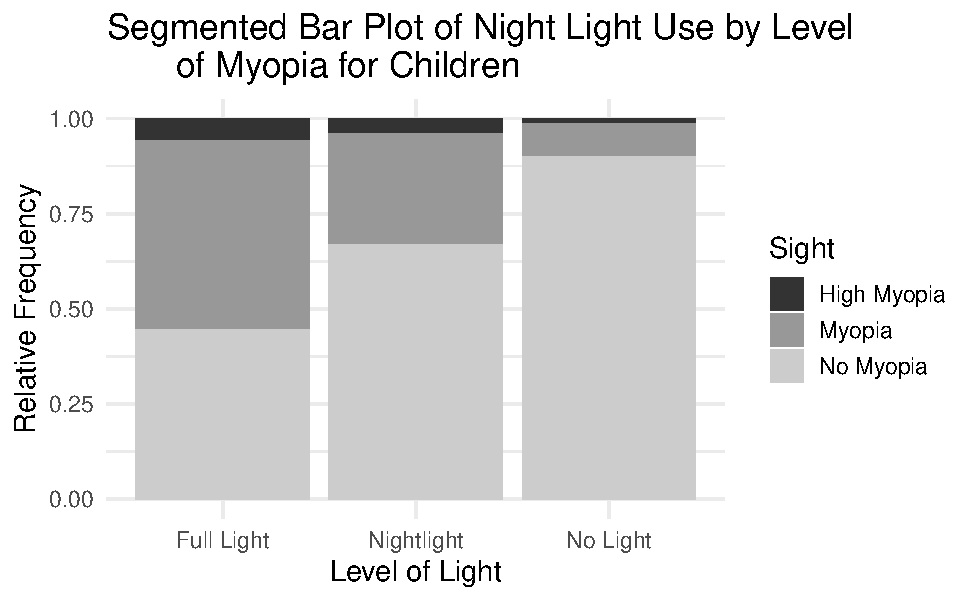
\includegraphics[width=0.6\linewidth]{03-OCA02-EDA_files/figure-latex/unnamed-chunk-8-1} \end{center}

\begin{enumerate}
\def\labelenumi{\arabic{enumi}.}
\setcounter{enumi}{9}
\tightlist
\item
  From the segmented bar plot, which level of light has the highest proportion of \texttt{No\ Myopia}?
\end{enumerate}

\vspace{0.5in}

\newpage

We could also create a mosaic plot of the data, shown below.

\begin{Shaded}
\begin{Highlighting}[]
\NormalTok{myopia}\SpecialCharTok{$}\NormalTok{Sight }\OtherTok{\textless{}{-}} \FunctionTok{factor}\NormalTok{(myopia}\SpecialCharTok{$}\NormalTok{Sight, }\AttributeTok{levels =} \FunctionTok{c}\NormalTok{(}\StringTok{"No Myopia"}\NormalTok{, }\StringTok{"Myopia"}\NormalTok{, }\StringTok{"High Myopia"}\NormalTok{))}
\NormalTok{myopia }\SpecialCharTok{\%\textgreater{}\%} \CommentTok{\#Data set piped into...}
  \FunctionTok{ggplot}\NormalTok{() }\SpecialCharTok{+}   \CommentTok{\#This specifies the variables}
  \FunctionTok{geom\_mosaic}\NormalTok{(}\FunctionTok{aes}\NormalTok{(}\AttributeTok{x=}\FunctionTok{product}\NormalTok{(Light), }\AttributeTok{fill =}\NormalTok{ Sight)) }\SpecialCharTok{+}  \CommentTok{\#Tell it to make a mosaic plot}
  \FunctionTok{labs}\NormalTok{(}\AttributeTok{title =} \StringTok{"Mosaic Plot of Night Light Use by Level of Myopia"}\NormalTok{, }\CommentTok{\#Make sure to title your plot }
       \AttributeTok{x =} \StringTok{"Level of Light"}\NormalTok{,   }\CommentTok{\#Label the x axis}
       \AttributeTok{y =} \StringTok{""}\NormalTok{) }\SpecialCharTok{+}  \CommentTok{\#Remove y axis label}
  \FunctionTok{scale\_fill\_grey}\NormalTok{(}\AttributeTok{guide =} \FunctionTok{guide\_legend}\NormalTok{(}\AttributeTok{reverse =} \ConstantTok{TRUE}\NormalTok{))  }\CommentTok{\#Make figure color}
\end{Highlighting}
\end{Shaded}

\begin{center}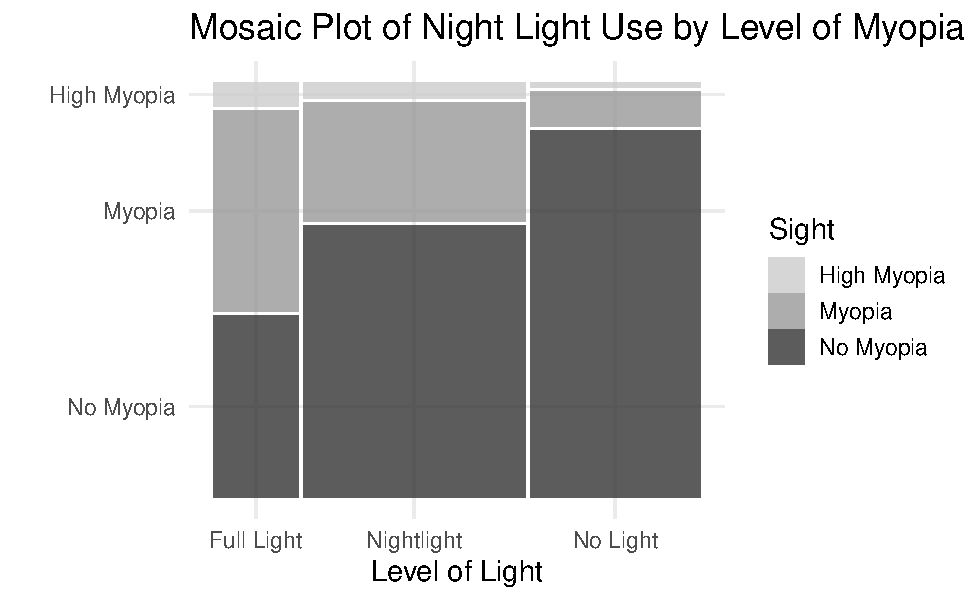
\includegraphics[width=0.6\linewidth]{03-OCA02-EDA_files/figure-latex/unnamed-chunk-9-1} \end{center}

\begin{enumerate}
\def\labelenumi{\arabic{enumi}.}
\setcounter{enumi}{10}
\tightlist
\item
  What is similar and what is different between the segmented bar chart and the mosaic bar chart?
\end{enumerate}

\vspace{1in}

\begin{enumerate}
\def\labelenumi{\arabic{enumi}.}
\setcounter{enumi}{11}
\tightlist
\item
  Explain why the bar for \texttt{Nightlight} is the widest in the mosaic plot.
\end{enumerate}

\vspace{0.8in}

\newpage

\hypertarget{take-home-messages-4}{%
\subsection{Take-home messages}\label{take-home-messages-4}}

\begin{enumerate}
\def\labelenumi{\arabic{enumi}.}
\item
  Bar charts can be used to graphically display a single categorical variable either as counts or proportions. Segmented bar charts and mosaic plots are used to display two categorical variables.
\item
  Segmented bar charts always have a scale from 0 -- 100\%. The bars represent the outcomes of the explanatory variable. Each bar is segmented by the response variable. If the heights of each segment are the same for each bar there is no association between variables.
\item
  Mosaic plots are similar to segmented bar charts but the widths of the bars also show the number of observations within each outcome. This allows assessment of the relative sizes of the levels of one variable in assessing changes in relative distributions of the levels of the other variable and the proportions of the totals in each combination of levels.
\end{enumerate}

\hypertarget{additional-notes-4}{%
\subsection{Additional notes}\label{additional-notes-4}}

Use this space to summarize your thoughts and take additional notes on today's activity and material covered.

\newpage

\hypertarget{activity-3-imdb-movie-reviews-displaying-quantitative-variables}{%
\section{Activity 3: IMDb Movie Reviews --- Displaying Quantitative Variables}\label{activity-3-imdb-movie-reviews-displaying-quantitative-variables}}

\setstretch{1}

\hypertarget{learning-outcomes-5}{%
\subsection{Learning outcomes}\label{learning-outcomes-5}}

\begin{itemize}
\item
  Identify and create appropriate summary statistics and plots
  given a data set or research question for quantitative data.
\item
  Interpret the following summary statistics in context:
  median, lower quartile, upper quartile,
  standard deviation, interquartile range.
\end{itemize}

\hypertarget{terminology-review-5}{%
\subsection{Terminology review}\label{terminology-review-5}}

In today's activity, we will review summary measures and plots for quantitative variables. Some terms covered in this activity are:

\begin{itemize}
\item
  Two measures of center: mean, median
\item
  Two measures of spread (variability): standard deviation, interquartile range (IQR)
\item
  Types of graphs: box plots, dot plots, histograms
\item
  Identify and create appropriate summary statistics and plots given a data set or research question for a single categorical and a single quantitative variable.
\item
  Interpret the following summary statistics in context:
  median, lower quartile, upper quartile,
  standard deviation, interquartile range.
\item
  Given a plot or set of plots, describe and compare the distribution(s)
  of a single quantitative variable
  (center, variability, shape, outliers).
\end{itemize}

To review these concepts, see Chapter 5 in the textbook.

\hypertarget{movies-released-in-2016}{%
\subsection{Movies released in 2016}\label{movies-released-in-2016}}

A data set was collected on movies released in 2016 ({``{IMDb} Movies Extensive Dataset''} 2016). Here is a list of some of the variables collected on the observational units, movies released in 2016.

\begin{longtable}[]{@{}
  >{\raggedright\arraybackslash}p{(\columnwidth - 2\tabcolsep) * \real{0.2353}}
  >{\raggedright\arraybackslash}p{(\columnwidth - 2\tabcolsep) * \real{0.7647}}@{}}
\toprule\noalign{}
\begin{minipage}[b]{\linewidth}\raggedright
\textbf{Variable}
\end{minipage} & \begin{minipage}[b]{\linewidth}\raggedright
\textbf{Description}
\end{minipage} \\
\midrule\noalign{}
\endhead
\bottomrule\noalign{}
\endlastfoot
\texttt{budget\_mil} & Amount of money (in US \$ millions) budgeted for the production of the movie \\
\texttt{revenue\_mil} & Amount of money (in US \$ millions) the movie made after release \\
\texttt{duration} & Length of the movie (in minutes) \\
\texttt{content\_rating} & Rating of the movie (\texttt{G}, \texttt{PG}, \texttt{PG-13}, \texttt{R}, \texttt{Not\ Rated}) \\
\texttt{imdb\_score} & IMDb user rating score from 1 to 10 \\
\texttt{genres} & Categories the movie falls into (e.g., Action, Drama, etc.) \\
\texttt{facebook\_likes} & Number of likes a movie receives on Facebook \\
\end{longtable}

\newpage

\hypertarget{summarizing-a-single-quantitative-variable}{%
\subsubsection*{Summarizing a single quantitative variable}\label{summarizing-a-single-quantitative-variable}}
\addcontentsline{toc}{subsubsection}{Summarizing a single quantitative variable}

The \texttt{favstats()} function from the \texttt{mosaic} package gives the summary statistics for a quantitative variable. The \texttt{R} output below provides the summary statistics for the variable \texttt{imdb\_score}. The summary statistics provided are the two measures of center (mean and median) and two measures of spread (standard deviation and the quartile values to calculate the IQR) for IMDb score.

\begin{itemize}
\tightlist
\item
  Highlight and run lines 1 -- 9 in the provided \texttt{R} script file to load the data set. Check that the summary statistics match the output given in the coursepack.
\end{itemize}

\begin{Shaded}
\begin{Highlighting}[]
\CommentTok{\# Read in data set}
\NormalTok{movies }\OtherTok{\textless{}{-}} \FunctionTok{read.csv}\NormalTok{(}\StringTok{"https://math.montana.edu/courses/s216/data/Movies2016.csv"}\NormalTok{) }
\NormalTok{movies }\SpecialCharTok{\%\textgreater{}\%} \CommentTok{\# Data set piped into...}
  \FunctionTok{summarise}\NormalTok{(}\FunctionTok{favstats}\NormalTok{(imdb\_score)) }\CommentTok{\# Apply favstats function to imdb\_score}
\end{Highlighting}
\end{Shaded}

\begin{verbatim}
#>   min   Q1 median  Q3 max     mean       sd  n missing
#> 1 3.4 5.65    6.4 7.1 8.2 6.309783 1.086689 92       0
\end{verbatim}

\begin{enumerate}
\def\labelenumi{\arabic{enumi}.}
\tightlist
\item
  Report the values for the two measures of center (mean and median).
\end{enumerate}

\vspace{0.5in}

\begin{enumerate}
\def\labelenumi{\arabic{enumi}.}
\setcounter{enumi}{1}
\tightlist
\item
  Calculate the interquartile range (IQR = Q3 \(-\) Q1) of IMDb scores.
\end{enumerate}

\vspace{0.5in}

\begin{enumerate}
\def\labelenumi{\arabic{enumi}.}
\setcounter{enumi}{2}
\tightlist
\item
  Report the value of the standard deviation and interpret this value in context of the problem.
  \vspace{0.8in}
\end{enumerate}

\hypertarget{displaying-a-single-quantitative-variable}{%
\subsubsection*{Displaying a single quantitative variable}\label{displaying-a-single-quantitative-variable}}
\addcontentsline{toc}{subsubsection}{Displaying a single quantitative variable}

There are three type of plots used to plot a single quantitative variable: a dotplot, a histogram or a boxplot. A dotplot of IMDb scores would plot a dot for the IMDb score for each movie released in 2016.

We will create both a histogram and a boxplot of the variable \texttt{IMDb}.

\begin{itemize}
\item
  Enter the name of the variable in both line 16 and line 23 for \texttt{variable} in the R script file.
\item
  Replace the word title for each plot (lines 18 and 25) between the quotations with a descriptive title. \textbf{A title should include: type of plot, variable or variables plotted, and observational units.}
\item
  Highlight and run lines 15 -- 27 to create a histogram and boxplot.
\end{itemize}

Notice that the \textbf{bin width} for the histogram is 0.5. For example the first bin consists of the number of movies in the data set with an IMDb score of 3.25 to 3.75. It is important to note that a movie with a IMDb score on the boundary of a bin will fall into the bin above it; for example, 4.75 would be counted in the bin 4.75--5.25.

\begin{Shaded}
\begin{Highlighting}[]
\NormalTok{movies }\SpecialCharTok{\%\textgreater{}\%} \CommentTok{\# Data set piped into...}
\FunctionTok{ggplot}\NormalTok{(}\FunctionTok{aes}\NormalTok{(}\AttributeTok{x =}\NormalTok{ variable)) }\SpecialCharTok{+}   \CommentTok{\# Name variable to plot}
  \FunctionTok{geom\_histogram}\NormalTok{(}\AttributeTok{binwidth =} \FloatTok{0.5}\NormalTok{) }\SpecialCharTok{+}  \CommentTok{\# Create histogram with specified binwidth}
  \FunctionTok{labs}\NormalTok{(}\AttributeTok{title =} \StringTok{"Title"}\NormalTok{, }\CommentTok{\# Title for plot}
       \AttributeTok{x =} \StringTok{"IMDb Score"}\NormalTok{, }\CommentTok{\# Label for x axis}
       \AttributeTok{y =} \StringTok{"Frequency"}\NormalTok{) }\CommentTok{\# Label for y axis}

\NormalTok{movies }\SpecialCharTok{\%\textgreater{}\%} \CommentTok{\# Data set piped into...}
\FunctionTok{ggplot}\NormalTok{(}\FunctionTok{aes}\NormalTok{(}\AttributeTok{x =}\NormalTok{ variable)) }\SpecialCharTok{+}   \CommentTok{\# Name variable to plot}
  \FunctionTok{geom\_boxplot}\NormalTok{() }\SpecialCharTok{+}  \CommentTok{\# Create histogram with specified binwidth}
  \FunctionTok{labs}\NormalTok{(}\AttributeTok{title =} \StringTok{"Title"}\NormalTok{, }\CommentTok{\# Title for plot}
       \AttributeTok{x =} \StringTok{"IMDb Score"}\NormalTok{, }\CommentTok{\# Label for x axis}
       \AttributeTok{y =} \StringTok{""}\NormalTok{) }\CommentTok{\# Remove y axis label}
\end{Highlighting}
\end{Shaded}

\begin{enumerate}
\def\labelenumi{\arabic{enumi}.}
\setcounter{enumi}{3}
\tightlist
\item
  What is the shape of the distribution of IMDb scores?
\end{enumerate}

\vspace{0.2in}

\begin{enumerate}
\def\labelenumi{\arabic{enumi}.}
\setcounter{enumi}{4}
\tightlist
\item
  Which range of IMDb scores have the highest frequency?
\end{enumerate}

\vspace{0.2in}

\begin{enumerate}
\def\labelenumi{\arabic{enumi}.}
\setcounter{enumi}{5}
\tightlist
\item
  Sketch the boxplot created and identify the values of the 5-number summary (minimum value, Q1, median, Q3, maximum value) on the plot. Use the following formulas to find the invisible fence on both ends of the distribution. Draw a dotted line at the invisible fence to show how the outliers were found.
\end{enumerate}

\[\text{Lower Fence: values} \le \text{Q}1 - 1.5\times\text{IQR}\]

\[\text{Upper Fence: values} \ge \text{Q}3 + 1.5\times\text{IQR}\]
\vspace{1.8in}

\hypertarget{summary-statistics-for-a-single-categorical-and-single-quantitative-variable}{%
\subsubsection*{Summary statistics for a single categorical and single quantitative Variable}\label{summary-statistics-for-a-single-categorical-and-single-quantitative-variable}}
\addcontentsline{toc}{subsubsection}{Summary statistics for a single categorical and single quantitative Variable}

Is there an association between content rating and budget for movies released in 2016? To use the \texttt{favstats()} function in the mosaic package with two variables, we will enter the variables as a formula, response\textasciitilde explanatory. This function will give the summary statistics for budget for each content rating.

\begin{itemize}
\tightlist
\item
  Highlight and run lines 31--33 in the provided \texttt{R} script file and check that the summary statistics match those provided in the coursepack.
\end{itemize}

\begin{Shaded}
\begin{Highlighting}[]
\NormalTok{movies }\SpecialCharTok{\%\textgreater{}\%} \CommentTok{\# Data set piped into...}
  \FunctionTok{filter}\NormalTok{(content\_rating }\SpecialCharTok{!=} \StringTok{"Not Rated"}\NormalTok{) }\SpecialCharTok{\%\textgreater{}\%} \CommentTok{\# Remove Not Rated movies}
  \FunctionTok{reframe}\NormalTok{(}\FunctionTok{favstats}\NormalTok{(budget\_mil}\SpecialCharTok{\textasciitilde{}}\NormalTok{content\_rating)) }\CommentTok{\# Find the summary measures for each content rating}
\end{Highlighting}
\end{Shaded}

\begin{verbatim}
#>   content_rating min    Q1 median      Q3 max     mean       sd  n missing
#> 1             PG 0.5 11.00   74.0 151.250 175 86.54167 71.52795 12       0
#> 2          PG-13 0.0 17.25   33.5 138.750 250 74.17500 74.15190 46       0
#> 3              R 0.0  7.75   19.5  29.625  60 21.09375 16.99926 32       0
\end{verbatim}

\begin{enumerate}
\def\labelenumi{\arabic{enumi}.}
\setcounter{enumi}{6}
\tightlist
\item
  Which content rating has the largest IQR?
\end{enumerate}

\vspace{0.8in}

\begin{enumerate}
\def\labelenumi{\arabic{enumi}.}
\setcounter{enumi}{7}
\tightlist
\item
  Report the mean budget amount for the PG rating. Use appropriate notation.
\end{enumerate}

\vspace{0.3in}

\begin{enumerate}
\def\labelenumi{\arabic{enumi}.}
\setcounter{enumi}{8}
\tightlist
\item
  Report the mean budget amount for the R rating. Use appropriate notation.
\end{enumerate}

\vspace{0.3in}

\begin{enumerate}
\def\labelenumi{\arabic{enumi}.}
\setcounter{enumi}{9}
\tightlist
\item
  Calculate the difference in mean budget amount for movies released in 2016 with a PG rating minus those with a R rating. Use appropriate notation with informative subscripts.
\end{enumerate}

\vspace{0.8in}

\begin{enumerate}
\def\labelenumi{\arabic{enumi}.}
\setcounter{enumi}{10}
\tightlist
\item
  Interpret the difference in means calculated in question 10 in context of the problem.
\end{enumerate}

\vspace{0.5in}

\hypertarget{displaying-a-single-categorical-and-single-quantitative-variable}{%
\subsubsection*{Displaying a single categorical and single quantitative variable}\label{displaying-a-single-categorical-and-single-quantitative-variable}}
\addcontentsline{toc}{subsubsection}{Displaying a single categorical and single quantitative variable}

The boxplot of movie budgets (in millions) by content rating is plotted using the code below.

\begin{itemize}
\item
  Enter the variable \texttt{budget\_mil} for \texttt{response} and the variable \texttt{content\_rating} for explanatory at line 40.
\item
  Highlight and run code lines 38--44. This plot compares the budget for different levels of content rating.
\end{itemize}

\begin{Shaded}
\begin{Highlighting}[]
\NormalTok{movies }\SpecialCharTok{\%\textgreater{}\%}  \CommentTok{\# Data set piped into...}
  \FunctionTok{filter}\NormalTok{(content\_rating }\SpecialCharTok{!=} \StringTok{"Not Rated"}\NormalTok{) }\SpecialCharTok{\%\textgreater{}\%} \CommentTok{\# Remove Not Rated movies}
  \FunctionTok{ggplot}\NormalTok{(}\FunctionTok{aes}\NormalTok{(}\AttributeTok{y =}\NormalTok{ response, }\AttributeTok{x =}\NormalTok{ explanatory))}\SpecialCharTok{+}  \CommentTok{\# Identify variables}
  \FunctionTok{geom\_boxplot}\NormalTok{()}\SpecialCharTok{+}  \CommentTok{\# Tell it to make a box plot}
  \FunctionTok{labs}\NormalTok{(}\AttributeTok{title =} \StringTok{"Side{-}by{-}side Box Plot of Budget by Content Rating for Movies Released in 2016"}\NormalTok{,  }
       \CommentTok{\# Title}
       \AttributeTok{x =} \StringTok{"Content Rating"}\NormalTok{,    }\CommentTok{\# x{-}axis label}
       \AttributeTok{y =} \StringTok{"Budget (in Millions)"}\NormalTok{)  }\CommentTok{\# y{-}axis label}
\end{Highlighting}
\end{Shaded}

\begin{enumerate}
\def\labelenumi{\arabic{enumi}.}
\setcounter{enumi}{11}
\tightlist
\item
  Sketch the box plots created using the \texttt{R} code.
\end{enumerate}

\vspace{3in}

\newpage

\begin{enumerate}
\def\labelenumi{\arabic{enumi}.}
\setcounter{enumi}{12}
\tightlist
\item
  Answer the following questions about the box plots created.
\end{enumerate}

\begin{enumerate}
\def\labelenumi{\alph{enumi}.}
\item
  Which content rating has the highest center?
  \vspace{0.2in}
\item
  Which content rating has the largest spread?
  \vspace{0.2in}
\item
  Which content rating has the most skewed distribution?
  \vspace{0.2in}
\item
  Fifty percent of movies released in 2016 with a PG-13 content rating fall below what value? What is the name of this value?
  \vspace{0.4in}
\item
  What is the value for the first quartile (Q1) for the PG-13 rating? Interpret this value in context.
  \vspace{.8in}
\end{enumerate}

\hypertarget{take-home-messages-5}{%
\subsection{Take-home messages}\label{take-home-messages-5}}

\begin{enumerate}
\def\labelenumi{\arabic{enumi}.}
\item
  Histograms, box plots, and dot plots can all be used to graphically display a single quantitative variable.
\item
  The box plot is created using the five number summary: minimum value, quartile 1, median, quartile 3, and maximum value. Values in the data set that are less than \(\text{Q}_1 - 1.5\times \text{IQR}\) and greater than \(\text{Q}_3 + 1.5\times \text{IQR}\) are considered outliers and are graphically represented by a dot outside of the whiskers on the box plot.
\item
  Data should be summarized numerically and displayed graphically to give us information about the study.
\item
  When comparing distributions of quantitative variables we look at the shape, center, spread, and for outliers. There are two measures of center: mean and the median and two measures of spread: standard deviation and the interquartile range, IQR = Q3 \(-\) Q1.
\end{enumerate}

\hypertarget{additional-notes-5}{%
\subsection{Additional notes}\label{additional-notes-5}}

Use this space to summarize your thoughts and take additional notes on today's activity and material covered.

\newpage

\hypertarget{week-3-lab-ipeds}{%
\section{Week 3 Lab: IPEDs}\label{week-3-lab-ipeds}}

\setstretch{1}

\hypertarget{learning-outcomes-6}{%
\subsection{Learning outcomes}\label{learning-outcomes-6}}

\begin{itemize}
\item
  Identify and create appropriate summary statistics and plots
  given a data set or research question for quantitative data.
\item
  Interpret the following summary statistics in context:
  median, lower quartile, upper quartile,
  standard deviation, interquartile range.
\end{itemize}

\hypertarget{terminology-review-6}{%
\subsection{Terminology review}\label{terminology-review-6}}

In today's lab, we will review summary measures and plots for quantitative variables. Some terms covered in this activity are:

\begin{itemize}
\item
  Two measures of center: mean, median
\item
  Two measures of spread (variability): standard deviation, interquartile range (IQR)
\item
  Types of graphs: box plots, dot plots, histograms
\item
  Identify and create appropriate summary statistics and plots given a data set or research question for a single categorical and a single quantitative variable.
\item
  Interpret the following summary statistics in context:
  median, lower quartile, upper quartile,
  standard deviation, interquartile range.
\item
  Given a plot or set of plots, describe and compare the distribution(s)
  of a single quantitative variable
  (center, variability, shape, outliers).
\end{itemize}

To review these concepts, see Chapter 5 in the textbook.

\hypertarget{the-integrated-postsecondary-education-data-system-ipeds}{%
\subsection{The Integrated Postsecondary Education Data System (IPEDS)}\label{the-integrated-postsecondary-education-data-system-ipeds}}

Upload and open the provided R script file for the week 3 lab to answer the following questions. \textbf{Remember bolded questions will be answered on Gradescope for your group.}

These data are on a subset of institutions that met the following selection criteria (Education Statistics 2018):

\begin{itemize}
\item
  Degree granting
\item
  United States only
\item
  Title IV participating
\item
  Not for profit
\item
  2-year or 4-year or above
\item
  Has full-time first-time undergraduates
\item
  Note that several variables have missing values for some institutions (denoted by ``NA'').
\end{itemize}

\begin{center}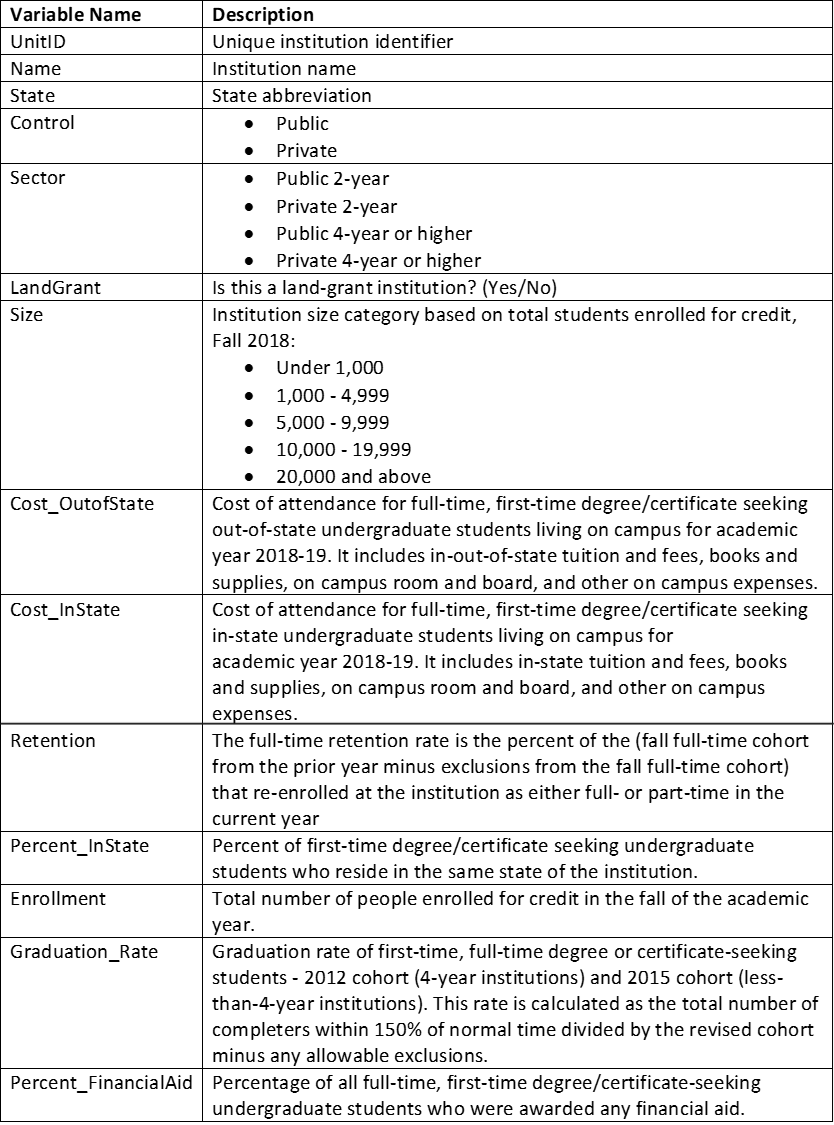
\includegraphics[width=0.77\linewidth]{images/IPEDS_Description} \end{center}

\hypertarget{summary-statistics-for-a-single-quantitative-variable}{%
\subsubsection*{Summary statistics for a single quantitative variable}\label{summary-statistics-for-a-single-quantitative-variable}}
\addcontentsline{toc}{subsubsection}{Summary statistics for a single quantitative variable}

Look through the provided chart above showing the description of variables measured. The UnitID and Name are identifiers for each observational unit, \emph{US degree granting institutions in 2018}.

\begin{enumerate}
\def\labelenumi{\arabic{enumi}.}
\tightlist
\item
  Identify in the chart above which variables collected on the US institutions are categorical (C) and which variables are quantitative (Q).
\end{enumerate}

\newpage

In the previous activities this week, the code was provided to import the data set needed directly from the Stat 216 website. Follow these steps to upload and import the data set for today's lab.

\begin{itemize}
\item
  Download the provided data set \texttt{IPED\_Data\_2018} from D2L
\item
  Upload the data set \texttt{IPEDS\_Data\_2018} to the RStudio server using the same steps to upload the R script file.
\item
  Click on ``Import Dataset'' in the Environment tab in the upper right hand corner.
\item
  Choose ``From Text(base)'' in the drop-down menu and select the correct csv file.
\item
  Be sure that ``Yes'' is selected next to ``Heading'' in the pop-up screen. Click ``Import''.
\item
  To view the data set, click on the data set name (\texttt{IPEDS\_Data\_2018}). Verify that that column names match the first column in the chart on the previous page. If the columns are named V1, V2, V3\ldots etc, you did not select ``Yes'' for ``Heading''.
\end{itemize}

Teams will also need the R script file for this week's lab.

\begin{itemize}
\item
  Download the provided R script file from D2L
\item
  Upload the R script file to the RStudio server
\item
  Enter the name of the data set (see the environment tab) for \texttt{datasetname} in the R script file in line 9.
\item
  We will look at the retention rates for the 4-year institutions only. Enter the variable name \texttt{Retention} for \texttt{variable} in line 15.
\item
  Highlight and run lines 1 -- 15. \textbf{Note that the two lines of code (lines 10 and 12) are filtering to remove the 2-year institutions so we are only assessing Public 4-year and Private 4-year institutions.}
\end{itemize}

The \texttt{favstats()} function from the \texttt{mosaic} package gives the summary statistics for a quantitative variable. The summary statistics give the two measures of center and two measures of spread for retention rates for 4-year institutions.

\begin{Shaded}
\begin{Highlighting}[]
\NormalTok{IPEDS }\OtherTok{\textless{}{-}}\NormalTok{ datasetname }\CommentTok{\#Creates the object IPEDS }
\NormalTok{IPEDS }\OtherTok{\textless{}{-}}\NormalTok{ IPEDS }\SpecialCharTok{\%\textgreater{}\%}
  \FunctionTok{filter}\NormalTok{(Sector }\SpecialCharTok{!=} \StringTok{"Public 2{-}year"}\NormalTok{) }\CommentTok{\#Filters the data set to remove Public 2{-}year}
\NormalTok{IPEDS }\OtherTok{\textless{}{-}}\NormalTok{ IPEDS }\SpecialCharTok{\%\textgreater{}\%}
  \FunctionTok{filter}\NormalTok{(Sector }\SpecialCharTok{!=} \StringTok{"Private 2{-}year"}\NormalTok{) }\CommentTok{\#Filters the data set to remove Private 2{-}year}
\NormalTok{IPEDS }\SpecialCharTok{\%\textgreater{}\%}
  \FunctionTok{summarise}\NormalTok{(}\FunctionTok{favstats}\NormalTok{(variable)) }\CommentTok{\#Gives the summary statistics}
\end{Highlighting}
\end{Shaded}

\begin{enumerate}
\def\labelenumi{\arabic{enumi}.}
\setcounter{enumi}{1}
\tightlist
\item
  Identify the observational units for this study after removing the 2-year institutions.
\end{enumerate}

\vspace{0.3in}

\begin{enumerate}
\def\labelenumi{\arabic{enumi}.}
\setcounter{enumi}{2}
\tightlist
\item
  \textbf{Report the value for quartile 3 and interpret this value in context of the study.}
\end{enumerate}

\vspace{0.8in}

\begin{enumerate}
\def\labelenumi{\arabic{enumi}.}
\setcounter{enumi}{3}
\tightlist
\item
  Report and interpret the value of the standard deviation.
\end{enumerate}

\vspace{0.8in}

\begin{enumerate}
\def\labelenumi{\arabic{enumi}.}
\setcounter{enumi}{4}
\tightlist
\item
  How many missing values are there? What does this indicate?
\end{enumerate}

\vspace{0.3in}

\hypertarget{robust-statistics-1}{%
\subsubsection*{Robust Statistics}\label{robust-statistics-1}}
\addcontentsline{toc}{subsubsection}{Robust Statistics}

Let's examine how the presence of outliers affect the values of center and spread.

\begin{enumerate}
\def\labelenumi{\arabic{enumi}.}
\setcounter{enumi}{5}
\tightlist
\item
  Report the two measures of center (mean and median) for retention rates given in the R output.
\end{enumerate}

\vspace{0.4in}

\begin{enumerate}
\def\labelenumi{\arabic{enumi}.}
\setcounter{enumi}{6}
\tightlist
\item
  Report the value of the standard deviation and calculate the value of the IQR (two measures of spread) for retention rates from the R output.
\end{enumerate}

\vspace{0.4in}

To show the effect of outliers on the measures of center and spread, the smallest values of retention rate in the data set were increased by 30\%.

\begin{itemize}
\tightlist
\item
  Highlight and run lines 19--20 in the R script file.
\end{itemize}

\begin{Shaded}
\begin{Highlighting}[]
\NormalTok{IPEDS }\SpecialCharTok{\%\textgreater{}\%} \CommentTok{\# Data set piped into...}
  \FunctionTok{summarise}\NormalTok{(}\FunctionTok{favstats}\NormalTok{(Retention\_Inc))}
\end{Highlighting}
\end{Shaded}

\begin{enumerate}
\def\labelenumi{\arabic{enumi}.}
\setcounter{enumi}{7}
\tightlist
\item
  Report the two measures of center for this new data set.
\end{enumerate}

\vspace{0.4in}

\begin{enumerate}
\def\labelenumi{\arabic{enumi}.}
\setcounter{enumi}{8}
\tightlist
\item
  Report the two measures of spread for this new data set.
\end{enumerate}

\vspace{0.4in}

\begin{enumerate}
\def\labelenumi{\arabic{enumi}.}
\setcounter{enumi}{9}
\tightlist
\item
  \textbf{Which measure of center is robust to (not affected by) outliers? Explain your answer.}
\end{enumerate}

\vspace{0.5in}

\begin{enumerate}
\def\labelenumi{\arabic{enumi}.}
\setcounter{enumi}{10}
\tightlist
\item
  Which measure of spread is robust to outliers? Explain your answer.
\end{enumerate}

\vspace{0.5in}

\hypertarget{summarizing-a-single-categorical-and-single-quantitative-variable}{%
\subsubsection*{Summarizing a single categorical and single quantitative variable}\label{summarizing-a-single-categorical-and-single-quantitative-variable}}
\addcontentsline{toc}{subsubsection}{Summarizing a single categorical and single quantitative variable}

Is there a difference in retention rates for public and private 4-year institutions? In the next part of the activity we will compare retention rates for public and private 4-year institutions. Note that this variable (public or private) is labelled \texttt{Sector} in the data set.

\begin{enumerate}
\def\labelenumi{\arabic{enumi}.}
\setcounter{enumi}{11}
\tightlist
\item
  \textbf{Based on the research question, which variable will we treat as the explanatory variable? Response variable?}
\end{enumerate}

\vspace{0.8in}

\begin{itemize}
\item
  To assess the research question described before question 12, enter the name of the explanatory variable and the name of the response variable in lines 28 and 31 of the R script file. Remember that the variable name must be typed in EXACTLY as it is written in the data set.
\item
  Replace the word title (line 33) between the quotations with a descriptive title. \textbf{A title should include: type of plot, variable or variables plotted, and observational units.}
\item
  Highlight and run lines 27 -- 35 to find the summary statistics and create side by side boxplots of the data.
\item
  \textbf{Export and upload the side-by-side box plot to Gradescope for your group.}

  \begin{itemize}
  \item
    To export the graph: in the bottom right corner in the Plots tab, click on \texttt{Export}
  \item
    Choose \texttt{Save\ as\ Image.} Save the image as a png. This will save your graph to the server.
  \item
    In the \texttt{Files} tab, click on the box next to your saved image file, click \texttt{More} and choose \texttt{Export}. This will save your file to your downloads folder on your computer.
  \end{itemize}
\end{itemize}

\begin{Shaded}
\begin{Highlighting}[]
\NormalTok{IPEDS }\SpecialCharTok{\%\textgreater{}\%}  \CommentTok{\# Data set piped into...}
  \FunctionTok{reframe}\NormalTok{(}\FunctionTok{favstats}\NormalTok{(response}\SpecialCharTok{\textasciitilde{}}\NormalTok{explanatory)) }\CommentTok{\# Summary statistics for retention rates by sector}
\end{Highlighting}
\end{Shaded}

\begin{Shaded}
\begin{Highlighting}[]
\NormalTok{IPEDS }\SpecialCharTok{\%\textgreater{}\%}  \CommentTok{\# Data set piped into...}
  \FunctionTok{ggplot}\NormalTok{(}\FunctionTok{aes}\NormalTok{(}\AttributeTok{y =}\NormalTok{ response, }\AttributeTok{x =}\NormalTok{ explanatory))}\SpecialCharTok{+}  \CommentTok{\# Identify variables}
  \FunctionTok{geom\_boxplot}\NormalTok{()}\SpecialCharTok{+}  \CommentTok{\# Create box plot}
  \FunctionTok{labs}\NormalTok{(}\AttributeTok{title =} \StringTok{"title"}\NormalTok{,  }\CommentTok{\# Give your plot a title}
       \AttributeTok{x =} \StringTok{"Sector"}\NormalTok{,    }\CommentTok{\# x{-}axis label}
       \AttributeTok{y =} \StringTok{"Retention Rates"}\NormalTok{)  }\CommentTok{\# y{-}axis label}
\end{Highlighting}
\end{Shaded}

\begin{enumerate}
\def\labelenumi{\arabic{enumi}.}
\setcounter{enumi}{12}
\item
  \textbf{Compare the two boxplots.}

  Which type of university has the highest center?
  \vspace{0.3in}

  Largest spread?
  \vspace{0.3in}

  What is the shape of each distribution?
  \vspace{0.3in}

  Does either distribution have potential outliers?
  \vspace{0.3in}
\item
  Report the difference in mean retention rates for private and public universities. Use private minus public as the order of subtraction. Use the appropriate notation.
\end{enumerate}

\vspace{0.8in}

\begin{enumerate}
\def\labelenumi{\arabic{enumi}.}
\setcounter{enumi}{14}
\tightlist
\item
  Does there appear to be an association between retention rates and type of university? Explain your answer using the boxplots and summary statistic.
\end{enumerate}

\vspace{0.3in}

\hypertarget{summarizing-two-categorical-variables}{%
\subsubsection*{Summarizing two categorical variables}\label{summarizing-two-categorical-variables}}
\addcontentsline{toc}{subsubsection}{Summarizing two categorical variables}

Are private 4-year institutions smaller than public one? The following set of code will create a segmented bar plot of size of the institution by sector.

\begin{itemize}
\item
  Enter the variable \texttt{Sector} for explanatory and \texttt{Size} for response in line 41.
\item
  Highlight and run lines 40 - 46 in the R script file.
\end{itemize}

\begin{Shaded}
\begin{Highlighting}[]
\NormalTok{IPEDS }\SpecialCharTok{\%\textgreater{}\%}
  \FunctionTok{ggplot}\NormalTok{(}\FunctionTok{aes}\NormalTok{(}\AttributeTok{x=}\NormalTok{explanatory, }\AttributeTok{fill =}\NormalTok{ response)) }\SpecialCharTok{+} \CommentTok{\# Enter the explanatory and response variables}
  \FunctionTok{geom\_bar}\NormalTok{(}\AttributeTok{stat =} \StringTok{"count"}\NormalTok{, }\AttributeTok{position =} \StringTok{"fill"}\NormalTok{) }\SpecialCharTok{+} \CommentTok{\# Create a segmented bar plot}
  \FunctionTok{labs}\NormalTok{(}\AttributeTok{title =} \StringTok{"Segmented Bar Plot of Sector by Size for }
\StringTok{       4{-}year Institutions"}\NormalTok{, }\CommentTok{\# Title}
       \AttributeTok{x =} \StringTok{"Sector"}\NormalTok{, }\CommentTok{\# x{-}axis label}
       \AttributeTok{y =} \StringTok{"Relative Frequency"}\NormalTok{) }\CommentTok{\# y{-}axis label}
\end{Highlighting}
\end{Shaded}

\begin{enumerate}
\def\labelenumi{\arabic{enumi}.}
\setcounter{enumi}{15}
\tightlist
\item
  Does there appear to be an association between sector and size of 4-year institutions? Explain your answer using the plot.
\end{enumerate}

\vspace{0.5in}

\newpage

\hypertarget{exploring-multivariable-data}{%
\chapter{Exploring Multivariable Data}\label{exploring-multivariable-data}}

\hypertarget{lecture-notes-week-4-regression-and-correlation}{%
\section{Lecture Notes Week 4: Regression and Correlation}\label{lecture-notes-week-4-regression-and-correlation}}

\setstretch{1}

\hypertarget{summary-measures-and-plots-for-two-quantitative-variables}{%
\subsection*{Summary measures and plots for two quantitative variables}\label{summary-measures-and-plots-for-two-quantitative-variables}}
\addcontentsline{toc}{subsection}{Summary measures and plots for two quantitative variables}

\setstretch{1.5}

A \_\_\_\_\_\_\_\_\_\_\_\_\_\_\_\_\_\_ is used to display the relationship
between two \_\_\_\_\_\_\_\_\_\_\_\_\_\_\_\_\_\_\_ variables.

\setstretch{1}

Four characteristics of the scatterplot:

\begin{itemize}
\tightlist
\item
  Form:
\end{itemize}

\vspace{0.2in}

\begin{itemize}
\tightlist
\item
  Direction:
\end{itemize}

\vspace{0.2in}

\begin{itemize}
\tightlist
\item
  Strength:
\end{itemize}

\vspace{0.2in}

\begin{itemize}
\tightlist
\item
  Outliers:
\end{itemize}

\vspace{0.2in}

\rgi \rgi - Influential points: outliers that change the regression line; far from the line of regression

\rgi \rgi - High leverage points: outliers that are extreme in the x- axis; far from the mean of the x-axis

\setstretch{1.5}

The summary measures for two quantitative variables are:

\begin{itemize}
\item
  \begin{center}\rule{0.5\linewidth}{0.5pt}\end{center}
\item
  \begin{center}\rule{0.5\linewidth}{0.5pt}\end{center}
\item
  \begin{center}\rule{0.5\linewidth}{0.5pt}\end{center}
\end{itemize}

\setstretch{1}

\begin{itemize}
\item
  Least-squares regression line: \(\hat{y}=b_0+b_1\times x\) (put y and x in the context of the problem) or \(\widehat{response}=b_0+b_1 \times \text{explanatory}\)
\item
  \(\hat{y}\) or \(\widehat{\text{response}}\) is
\end{itemize}

\vspace{0.1in}

\begin{itemize}
\tightlist
\item
  \(b_0\) is
\end{itemize}

\vspace{0.1in}

\begin{itemize}
\tightlist
\item
  \(b_1\) is
\end{itemize}

\vspace{0.1in}

\begin{itemize}
\tightlist
\item
  \(x\) or explanatory is
\end{itemize}

\vspace{0.1in}

\setstretch{1.5}

\begin{itemize}
\item
  The estimates for the linear model output will give the value of the \_\_\_\_\_\_\_\_\_\_\_\_\_\_\_\_\_\_\_ and the \_\_\_\_\_\_\_\_\_\_\_\_\_\_.
\item
  Interpretation of slope: an increase in the \_\_\_\_\_\_\_\_\_\_\_\_\_ variable of 1 unit is associated with an increase/decrease in the \_\_\_\_\_\_\_\_\_\_\_\_\_\_\_\_ variable by the value of slope, on average.
\item
  Interpretation of the y-intercept: for a value of 0 for the \_\_\_\_\_\_\_\_\_\_\_\_\_ variable, the predicted value for the \_\_\_\_\_\_\_\_\_\_ variable would be the value of y-intercept.
\item
  We can predict values of the \_\_\_\_\_\_\_\_\_\_\_ variable by plugging in a given \_\_\_\_\_\_\_\_\_\_ variable value using the least squares equation line.
\item
  A prediction of a response variable value for an explanatory value outside the range of x values is called \_\_\_\_\_\_\_\_\_\_\_\_\_\_\_.
\item
  To find how far the predicted value deviates from the actual value we find the \_\_\_\_\_\_\_\_\_\_\_\_.
\end{itemize}

\vspace{0.3in}

\begin{itemize}
\item
  To find the least squares regression line the line with the \_\_\_\_\_\_\_\_\_\_ SSE is found.

  SSE =

  \begin{itemize}
  \tightlist
  \item
    To find SSE, the \_\_\_\_\_\_\_\_\_ for each data point is found, squared and all the squared residuals are summed together
  \end{itemize}
\end{itemize}

Correlation is always between the values of \_\_\_\_\_\_\_ and \_\_\_\_\_\_\_\_.

\begin{itemize}
\item
  Measures the \_\_\_\_\_\_\_\_\_\_\_\_\_ and \_\_\_\_\_\_\_\_\_\_\_\_\_\_ of the linear relationship between two quantitative variables.
\item
  The stronger the relationship between the variables the closer the value of \_\_\_\_\_\_\_\_\_\_\_\_\_\_\_ is to \_\_\_\_\_\_\_\_ or \_\_\_\_\_\_\_\_.
\item
  The sign gives the \_\_\_\_\_\_\_\_\_\_\_\_\_\_\_\_\_.
\end{itemize}

The coefficient of determination can be found by squaring the value of correlation, using the \_\_\_\_\_\_\_\_\_\_\_\_\_ for each variable or using the SSE (sum of squares error) and SST (sum of squares total)

\begin{itemize}
\item
  \(r^2 = (r)^2 = \frac{SST - SSE}{SST} = \frac{s^2_y - s^2_{residual}}{s^2_y}\)
\item
  The coefficient of determination measures the \_\_\_\_\_\_\_\_\_\_\_\_ of total variation in the \_\_\_\_\_\_\_\_\_\_\_ variable that is explained by the changes in the \_\_\_\_\_\_\_\_\_\_\_\_\_ variable.
\end{itemize}

Notation:

\begin{itemize}
\item
  Population slope:
\item
  Population correlation:
\item
  Sample slope:
\item
  Sample correlation:
\end{itemize}

\setstretch{1}

\vspace{1mm}

Example for class discussion: Data were collected from 1236 births between 1960 and 1967 in the San Francisco East Bay area to better understand what variables contributed to child birthweight, as children with low birthweight often suffer from an array of complications later in life ({``Child Health and Development Studies,''} n.d.). There were some missing values in the study and with those observations removed we have a total of 1223 births.

\begin{Shaded}
\begin{Highlighting}[]
\NormalTok{babies}\OtherTok{\textless{}{-}}\FunctionTok{read.csv}\NormalTok{(}\StringTok{"data/babies.csv"}\NormalTok{) }\SpecialCharTok{\%\textgreater{}\%}
    \FunctionTok{drop\_na}\NormalTok{(bwt) }\SpecialCharTok{\%\textgreater{}\%}
    \FunctionTok{drop\_na}\NormalTok{(gestation)}
\FunctionTok{glimpse}\NormalTok{(babies)}
\CommentTok{\#\textgreater{} Rows: 1,223}
\CommentTok{\#\textgreater{} Columns: 8}
\CommentTok{\#\textgreater{} $ case      \textless{}int\textgreater{} 1, 2, 3, 5, 6, 7, 8, 9, 10, 11, 12, 13, 14, 15, 16, 17, 18, \textasciitilde{}}
\CommentTok{\#\textgreater{} $ bwt       \textless{}int\textgreater{} 120, 113, 128, 108, 136, 138, 132, 120, 143, 140, 144, 141, \textasciitilde{}}
\CommentTok{\#\textgreater{} $ gestation \textless{}int\textgreater{} 284, 282, 279, 282, 286, 244, 245, 289, 299, 351, 282, 279, \textasciitilde{}}
\CommentTok{\#\textgreater{} $ parity    \textless{}int\textgreater{} 0, 0, 0, 0, 0, 0, 0, 0, 0, 0, 0, 0, 0, 0, 0, 0, 0, 0, 0, 0, \textasciitilde{}}
\CommentTok{\#\textgreater{} $ age       \textless{}int\textgreater{} 27, 33, 28, 23, 25, 33, 23, 25, 30, 27, 32, 23, 36, 30, 38, \textasciitilde{}}
\CommentTok{\#\textgreater{} $ height    \textless{}int\textgreater{} 62, 64, 64, 67, 62, 62, 65, 62, 66, 68, 64, 63, 61, 63, 63, \textasciitilde{}}
\CommentTok{\#\textgreater{} $ weight    \textless{}int\textgreater{} 100, 135, 115, 125, 93, 178, 140, 125, 136, 120, 124, 128, 9\textasciitilde{}}
\CommentTok{\#\textgreater{} $ smoke     \textless{}int\textgreater{} 0, 0, 1, 1, 0, 0, 0, 0, 1, 0, 1, 1, 1, 0, 0, 1, 1, 0, 1, 0, \textasciitilde{}}
\end{Highlighting}
\end{Shaded}

Here you see a glimpse of the data. The 1223 rows correspond to the sample size. The case variable is labeling each pregnancy 1 through 1223. Then 7 variables are recorded. birthweight (bwt), length of gestation in days, parity is called an indicator variable telling us if the pregnancy was a first pregnancy (labeled as 0) or not (labeled as 1) were recorded about the child and pregnancy. The age, height, and weight were recorded for the mother giving birth, as was smoke, another indicator variable where 0 means the mother did not smoke during pregnancy, and 1 indicates that she did smoke while pregnant.

The following shows a scatterplot of length of gestation as a predictor of birthweight.

\begin{Shaded}
\begin{Highlighting}[]
\NormalTok{babies }\SpecialCharTok{\%\textgreater{}\%} \CommentTok{\# Data set pipes into...}
\FunctionTok{ggplot}\NormalTok{(}\FunctionTok{aes}\NormalTok{(}\AttributeTok{x =}\NormalTok{ gestation, }\AttributeTok{y =}\NormalTok{ bwt))}\SpecialCharTok{+}  \CommentTok{\# Specify variables}
  \FunctionTok{geom\_point}\NormalTok{(}\AttributeTok{alpha=}\FloatTok{0.5}\NormalTok{) }\SpecialCharTok{+}  \CommentTok{\# Add scatterplot of points}
  \FunctionTok{labs}\NormalTok{(}\AttributeTok{x =} \StringTok{"number of days of gestation"}\NormalTok{,  }\CommentTok{\# Label x{-}axis}
       \AttributeTok{y =} \StringTok{"birthweight (oz)"}\NormalTok{,  }\CommentTok{\# Label y{-}axis}
       \AttributeTok{title =} \StringTok{"Scatterplot of Gestation vs. Birthweight for Births}
\StringTok{       between 1960 and 1967 in San Francisco"}\NormalTok{) }\SpecialCharTok{+} 
    \CommentTok{\# Be sure to title your plots with the type of plot, observational units, variable(s)}
  \FunctionTok{geom\_smooth}\NormalTok{(}\AttributeTok{method =} \StringTok{"lm"}\NormalTok{, }\AttributeTok{se =} \ConstantTok{FALSE}\NormalTok{) }\SpecialCharTok{+} \CommentTok{\# Add regression line}
    \FunctionTok{theme\_bw}\NormalTok{()}
\end{Highlighting}
\end{Shaded}

\begin{center}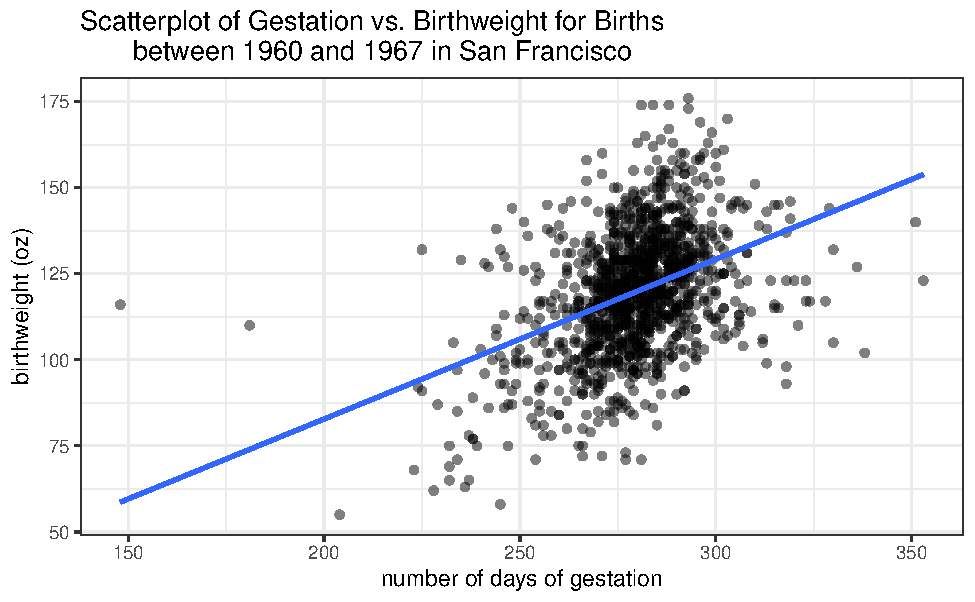
\includegraphics[width=0.8\linewidth]{04-LN04-two-quantitativeEDA_files/figure-latex/unnamed-chunk-2-1} \end{center}

Describe the scatterplot using the four characteristics of a scatterplot.

\vspace{1in}

The linear model output for this study is given below:

\begin{Shaded}
\begin{Highlighting}[]
\CommentTok{\# Fit linear model: y \textasciitilde{} x}
\NormalTok{babiesLM }\OtherTok{\textless{}{-}} \FunctionTok{lm}\NormalTok{(bwt }\SpecialCharTok{\textasciitilde{}}\NormalTok{ gestation, }\AttributeTok{data=}\NormalTok{babies)}
\FunctionTok{summary}\NormalTok{(babiesLM)}\SpecialCharTok{$}\NormalTok{coefficients }\CommentTok{\# Display coefficient summary}
\CommentTok{\#\textgreater{}                Estimate Std. Error   t value     Pr(\textgreater{}|t|)}
\CommentTok{\#\textgreater{} (Intercept) {-}10.0641842 8.32220357 {-}1.209317 2.267751e{-}01}
\CommentTok{\#\textgreater{} gestation     0.4642626 0.02974366 15.608793 3.224362e{-}50}
\end{Highlighting}
\end{Shaded}

Write the least squares equation of the line.

\vspace{0.6in}

Interpret the slope in context of the problem.

\vspace{0.6in}

Interpret the y-intercept in context of the problem.

\vspace{0.6in}

Predict the birthweight for a birth with a baby born at 310 days gestation.

\vspace{0.5in}

Calculate the residual for a birth of a baby with a birthweight of 151 ounces and born at 310 days gestation.

\vspace{0.5in}

Is this value (310, 151) above or below the line of regression? Did the line of regression overestimate or underestimate the birthweight?

\vspace{0.2in}

The following code creates a correlation matrix between different quantitative variables in the data set.

\begin{Shaded}
\begin{Highlighting}[]
\NormalTok{babies }\SpecialCharTok{\%\textgreater{}\%}
    \FunctionTok{select}\NormalTok{(}\FunctionTok{c}\NormalTok{(}\StringTok{"gestation"}\NormalTok{, }\StringTok{"age"}\NormalTok{, }\StringTok{"height"}\NormalTok{, }\StringTok{"weight"}\NormalTok{, }\StringTok{"bwt"}\NormalTok{)) }\SpecialCharTok{\%\textgreater{}\%}
    \FunctionTok{cor}\NormalTok{(}\AttributeTok{use=}\StringTok{"pairwise.complete.obs"}\NormalTok{) }\SpecialCharTok{\%\textgreater{}\%}
    \FunctionTok{round}\NormalTok{(}\DecValTok{3}\NormalTok{)}
\CommentTok{\#\textgreater{}           gestation    age height weight   bwt}
\CommentTok{\#\textgreater{} gestation     1.000 {-}0.056  0.064  0.022 0.408}
\CommentTok{\#\textgreater{} age          {-}0.056  1.000 {-}0.005  0.147 0.029}
\CommentTok{\#\textgreater{} height        0.064 {-}0.005  1.000  0.436 0.201}
\CommentTok{\#\textgreater{} weight        0.022  0.147  0.436  1.000 0.154}
\CommentTok{\#\textgreater{} bwt           0.408  0.029  0.201  0.154 1.000}
\end{Highlighting}
\end{Shaded}

\setstretch{1.5}

The value of correlation between gestation and birthweight is \_\_\_\_\_\_\_\_\_\_\_\_\_\_. This shows a \_\_\_\_\_\_\_\_\_\_\_, \_\_\_\_\_\_\_\_\_\_\_\_\_ relationship between gestation and birthweight.

\setstretch{1}

\begin{center}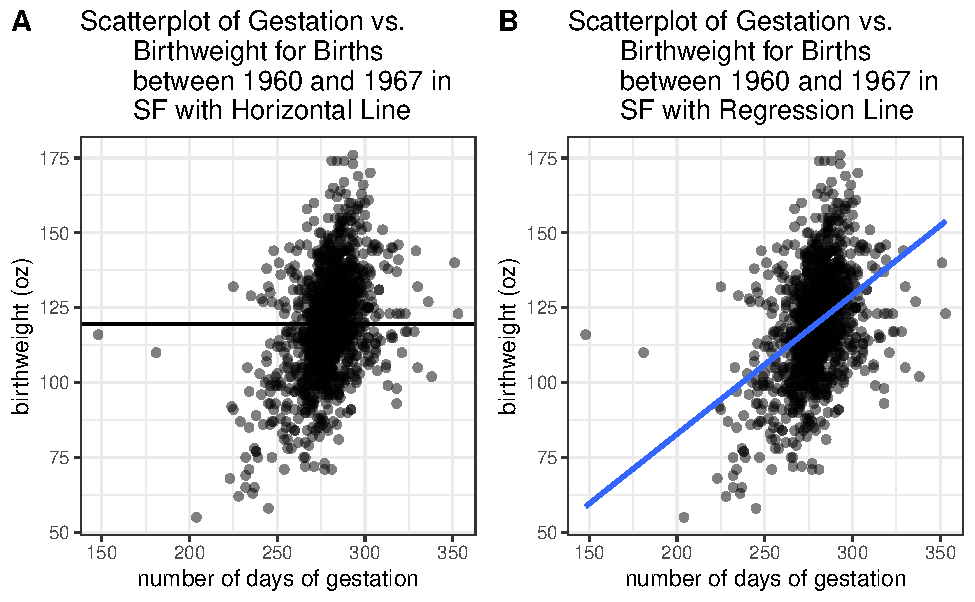
\includegraphics[width=0.7\linewidth]{04-LN04-two-quantitativeEDA_files/figure-latex/unnamed-chunk-6-1} \end{center}

The value for SST was calculated as 406753.48. The value for SSE was calculated as 339092.13.

Calculate the coefficient of determination between gestation and birthweight.

\vspace{0.3in}

Interpret the coefficient of determination between gestation and birthweight.

\vspace{0.5in}

\newpage

\hypertarget{multivariable-plots}{%
\subsubsection*{Multivariable plots}\label{multivariable-plots}}
\addcontentsline{toc}{subsubsection}{Multivariable plots}

Aesthetics: visual property of the objects in your plot

\setstretch{1.5}

\begin{itemize}
\item
  Position on the axes: groups for \_\_\_\_\_\_\_\_\_\_\_\_\_\_\_ variables, or a number line if the variable is \_\_\_\_\_\_\_\_\_\_\_\_\_\_\_\_\_
\item
  Color or shape - to represent \_\_\_\_\_\_\_\_\_\_\_\_\_\_\_ variables
\item
  Size - to represent \_\_\_\_\_\_\_\_\_\_\_\_\_\_\_\_ variables
\end{itemize}

\setstretch{1}

Adding the quantitative variable maternal age to the scatterplot between gestation and birthweight.

\begin{Shaded}
\begin{Highlighting}[]
\NormalTok{babies }\SpecialCharTok{\%\textgreater{}\%} \CommentTok{\# Data set pipes into...}
\FunctionTok{ggplot}\NormalTok{(}\FunctionTok{aes}\NormalTok{(}\AttributeTok{x =}\NormalTok{ gestation, }\AttributeTok{y =}\NormalTok{ bwt))}\SpecialCharTok{+}  \CommentTok{\# Specify variables}
  \FunctionTok{geom\_point}\NormalTok{(}\AttributeTok{alpha=}\FloatTok{0.5}\NormalTok{, }\AttributeTok{shape=}\DecValTok{1}\NormalTok{, }\FunctionTok{aes}\NormalTok{(}\AttributeTok{size=}\NormalTok{age)) }\SpecialCharTok{+}  \CommentTok{\# Add scatterplot of points}
  \FunctionTok{labs}\NormalTok{(}\AttributeTok{x =} \StringTok{"number of days of gestation"}\NormalTok{,  }\CommentTok{\# Label x{-}axis}
       \AttributeTok{y =} \StringTok{"birthweight (oz)"}\NormalTok{,  }\CommentTok{\# Label y{-}axis}
       \AttributeTok{title =} \StringTok{"Scatterplot of Gestation vs. Birthweight by Age }
\StringTok{       for Births between 1960 and 1967 in San Francisco"}\NormalTok{) }\SpecialCharTok{+} 
    \CommentTok{\# Be sure to title your plots}
  \FunctionTok{geom\_smooth}\NormalTok{(}\AttributeTok{method =} \StringTok{"lm"}\NormalTok{, }\AttributeTok{se =} \ConstantTok{FALSE}\NormalTok{)  }\CommentTok{\# Add regression line}
\end{Highlighting}
\end{Shaded}

\begin{center}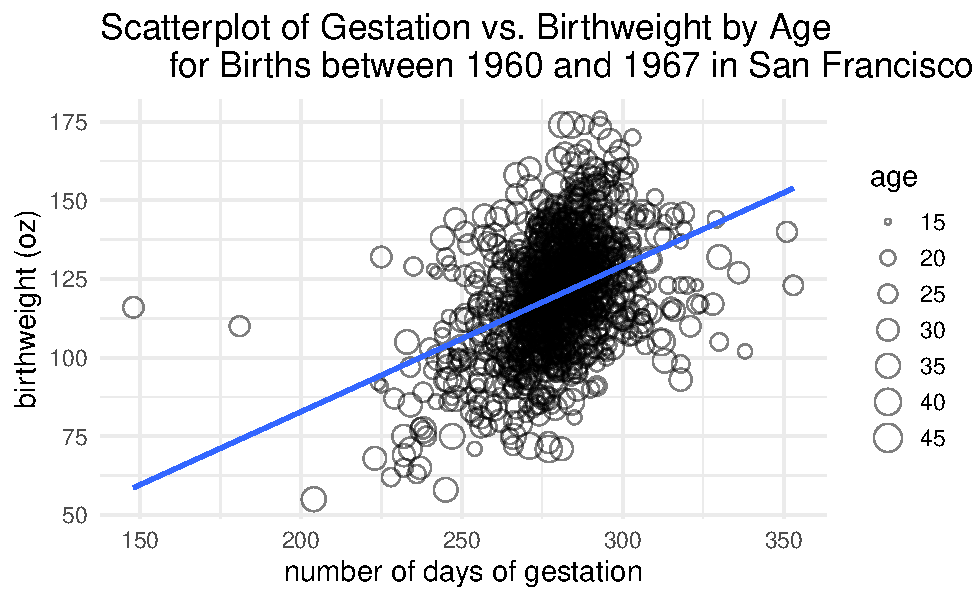
\includegraphics[width=0.8\linewidth]{04-LN04-two-quantitativeEDA_files/figure-latex/unnamed-chunk-7-1} \end{center}

\newpage

Let's add the categorical variable, whether a mother smoked, to the scatterplot between gestation and birthweight.

\begin{Shaded}
\begin{Highlighting}[]
\NormalTok{babies }\OtherTok{\textless{}{-}}\NormalTok{ babies }\SpecialCharTok{\%\textgreater{}\%} 
    \FunctionTok{mutate}\NormalTok{(}\AttributeTok{smoke =} \FunctionTok{factor}\NormalTok{(smoke)) }\SpecialCharTok{\%\textgreater{}\%}
    \FunctionTok{na.omit}\NormalTok{()}
           
\NormalTok{babies }\SpecialCharTok{\%\textgreater{}\%} \CommentTok{\# Data set pipes into...}
    \FunctionTok{ggplot}\NormalTok{(}\FunctionTok{aes}\NormalTok{(}\AttributeTok{x =}\NormalTok{ gestation, }\AttributeTok{y =}\NormalTok{ bwt, }\AttributeTok{color =}\NormalTok{ smoke))}\SpecialCharTok{+}  \CommentTok{\#Specify variables}
    \FunctionTok{geom\_point}\NormalTok{(}\FunctionTok{aes}\NormalTok{(}\AttributeTok{shape =}\NormalTok{ smoke), }\AttributeTok{size =} \DecValTok{2}\NormalTok{) }\SpecialCharTok{+}  \CommentTok{\#Add scatterplot of points}
    \FunctionTok{labs}\NormalTok{(}\AttributeTok{x =} \StringTok{"number of days of gestation"}\NormalTok{,  }\CommentTok{\#Label x{-}axis}
         \AttributeTok{y =} \StringTok{"birthweight (oz)"}\NormalTok{,  }\CommentTok{\#Label y{-}axis}
         \AttributeTok{title =} \StringTok{"Scatterplot of Gestation vs. Birthweight by }
\StringTok{         Smoking Status for Births between 1960 and 1967 }
\StringTok{         in San Francisco"}\NormalTok{) }\SpecialCharTok{+} 
    \CommentTok{\#Be sure to title your plots}
    \FunctionTok{geom\_smooth}\NormalTok{(}\AttributeTok{method =} \StringTok{"lm"}\NormalTok{, }\AttributeTok{se =} \ConstantTok{FALSE}\NormalTok{) }\SpecialCharTok{+} \CommentTok{\#Add regression line}
    \FunctionTok{scale\_color\_grey}\NormalTok{()}
\end{Highlighting}
\end{Shaded}

\begin{center}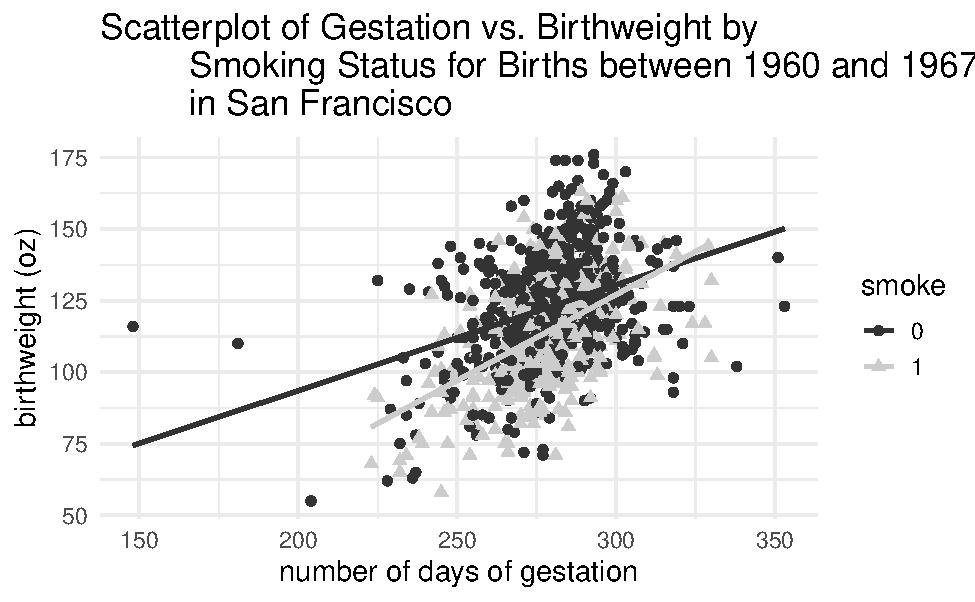
\includegraphics[width=0.8\linewidth]{04-LN04-two-quantitativeEDA_files/figure-latex/unnamed-chunk-8-1} \end{center}

Does the relationship between length of gestation and birthweight appear to depend upon maternal smoking status?

\vspace{1in}

Is the variable smoking status a potential confounding variable?

\vspace{1in}

Adding a categorical predictor:

\setstretch{1.5}

\begin{itemize}
\item
  Look at the regression line for each level of the \_\_\_\_\_\_\_\_\_\_\_\_\_\_
\item
  If the slopes are \_\_\_\_\_\_\_\_\_\_\_\_\_\_\_\_, the two predictor variables do not \_\_\_\_\_\_\_\_\_\_\_\_\_\_\_ to help explain the response
\item
  If the slopes \_\_\_\_\_\_\_\_\_\_\_\_\_\_\_\_\_, there is an interaction between the categorical predictor and the relationship between the two quantitative variables.
\end{itemize}

\setstretch{1}

\newpage

\hypertarget{out-of-class-activity-week-4-movie-profits-correlation-and-coefficient-of-determination}{%
\section{Out-of-Class Activity Week 4: Movie Profits --- Correlation and Coefficient of Determination}\label{out-of-class-activity-week-4-movie-profits-correlation-and-coefficient-of-determination}}

\setstretch{1}

\hypertarget{learning-outcomes-7}{%
\subsection{Learning outcomes}\label{learning-outcomes-7}}

\begin{itemize}
\item
  Identify and create appropriate summary statistics and plots
  given a data set with two quantitative variables.
\item
  Calculate and interpret \(r^2\), the coefficient of determination, in context of the problem.
\item
  Find the correlation coefficient from \texttt{R} output or from \(r^2\) and the sign of the slope.
\end{itemize}

\hypertarget{terminology-review-7}{%
\subsection{Terminology review}\label{terminology-review-7}}

In today's activity, we will review summary measures and plots for two quantitative variables. Some terms covered in this activity are:

\begin{itemize}
\item
  Correlation (\(r\))
\item
  Coefficient of determination (\(r\)-squared)
\end{itemize}

To review these concepts, see Chapter 6 in the textbook.

\hypertarget{movies-released-in-2016-1}{%
\subsection{Movies released in 2016}\label{movies-released-in-2016-1}}

A data set was collected on movies released in 2016 ({``{IMDb} Movies Extensive Dataset''} 2016). Here is a list of some of the variables collected on the observational units, movies released in 2016. (Note: both budget and revenue are measured in ``millions of dollars'' (\$MM).)

\begin{longtable}[]{@{}
  >{\raggedright\arraybackslash}p{(\columnwidth - 2\tabcolsep) * \real{0.2353}}
  >{\raggedright\arraybackslash}p{(\columnwidth - 2\tabcolsep) * \real{0.7647}}@{}}
\toprule\noalign{}
\begin{minipage}[b]{\linewidth}\raggedright
\textbf{Variable}
\end{minipage} & \begin{minipage}[b]{\linewidth}\raggedright
\textbf{Description}
\end{minipage} \\
\midrule\noalign{}
\endhead
\bottomrule\noalign{}
\endlastfoot
\texttt{budget\_mil} & Amount of money (\$MM) budgeted for the production of the movie \\
\texttt{revenue\_mil} & Amount of money (\$MM) the movie made after release \\
\texttt{duration} & Length of the movie (in minutes) \\
\texttt{content\_rating} & Rating of the movie (\texttt{G}, \texttt{PG}, \texttt{PG-13}, \texttt{R}, \texttt{Not\ Rated}) \\
\texttt{imdb\_score} & IMDb user rating score from 1 to 10 \\
\texttt{genres} & Categories the movie falls into (e.g., Action, Drama, etc.) \\
\texttt{facebook\_likes} & Number of likes a movie receives on Facebook \\
\end{longtable}

\newpage

\hypertarget{correlation}{%
\subsubsection*{Correlation}\label{correlation}}
\addcontentsline{toc}{subsubsection}{Correlation}

Correlation measures the strength and the direction of the linear relationship between two quantitative variables. The closer the value of correlation to \(+1\) or \(-1\), the stronger the linear relationship. Values close to zero indicate a very weak linear relationship between the two variables.

\begin{Shaded}
\begin{Highlighting}[]
\NormalTok{movies }\OtherTok{\textless{}{-}} \FunctionTok{read.csv}\NormalTok{(}\StringTok{"https://math.montana.edu/courses/s216/data/Movies2016.csv"}\NormalTok{) }\CommentTok{\# Reads in data set}
\NormalTok{movies }\SpecialCharTok{\%\textgreater{}\%}  \CommentTok{\# Data set pipes into}
  \FunctionTok{select}\NormalTok{(}\FunctionTok{c}\NormalTok{(}\StringTok{"budget\_mil"}\NormalTok{, }\StringTok{"revenue\_mil"}\NormalTok{, }
           \StringTok{"duration"}\NormalTok{, }\StringTok{"imdb\_score"}\NormalTok{, }
           \StringTok{"facebook\_likes"}\NormalTok{)) }\SpecialCharTok{\%\textgreater{}\%}
  \FunctionTok{cor}\NormalTok{(}\AttributeTok{use=}\StringTok{"pairwise.complete.obs"}\NormalTok{) }\SpecialCharTok{\%\textgreater{}\%}
  \FunctionTok{round}\NormalTok{(}\DecValTok{3}\NormalTok{)}
\end{Highlighting}
\end{Shaded}

\begin{verbatim}
#>                budget_mil revenue_mil duration imdb_score facebook_likes
#> budget_mil          1.000       0.686    0.463      0.292          0.678
#> revenue_mil         0.686       1.000    0.227      0.398          0.723
#> duration            0.463       0.227    1.000      0.261          0.438
#> imdb_score          0.292       0.398    0.261      1.000          0.309
#> facebook_likes      0.678       0.723    0.438      0.309          1.000
\end{verbatim}

\begin{enumerate}
\def\labelenumi{\arabic{enumi}.}
\item
  Explain why the correlation values on the diagonal are equal to 1.
  \vspace{0.8in}
\item
  Using the output above, ignoring the values of 1, which pair of variables have the \emph{strongest} correlation? What is the value of this correlation?
\end{enumerate}

\vspace{0.5in}

\begin{enumerate}
\def\labelenumi{\arabic{enumi}.}
\setcounter{enumi}{2}
\tightlist
\item
  What is the value of correlation between budget and revenue?
\end{enumerate}

\vspace{0.3in}

\hypertarget{coefficient-of-determination-squared-correlation}{%
\subsubsection*{Coefficient of determination (squared correlation)}\label{coefficient-of-determination-squared-correlation}}
\addcontentsline{toc}{subsubsection}{Coefficient of determination (squared correlation)}

Another summary measure used to explain the linear relationship between two quantitative variables is the coefficient of determination (\(r^2\)). The coefficient of determination, \(r^2\), can also be used to describe the strength of the linear relationship between two quantitative variables. The value of \(r^2\) (a value between 0 and 1) represents the \textbf{proportion of variation in the response that is explained by the least squares line with the explanatory variable}. There are two ways to calculate the coefficient of determination:

~~~Square the correlation coefficient: \(r^2 = (r)^2\)

~~~Use the variances of the response and the residuals: \(r^2 = \dfrac{s_y^2 - s_{RES}^2}{s_y^2} = \dfrac{SST - SSE}{SST}\)

\begin{enumerate}
\def\labelenumi{\arabic{enumi}.}
\setcounter{enumi}{3}
\tightlist
\item
  Use the correlation, \(r\), found in question 3 of the activity, to calculate the coefficient of determination between budget and revenue, \(r^2\).
\end{enumerate}

\vspace{.4in}

\newpage

\begin{enumerate}
\def\labelenumi{\arabic{enumi}.}
\setcounter{enumi}{4}
\tightlist
\item
  The variance of the response variable, revenue in \$MM, is about \(s_{revenue}^2 = 8024.261\) \$MM\(^2\) and the variability in the residuals is about \(s_{RES}^2 = 4244.832\) \$MM\(^2\). Use these values to calculate the coefficient of determination. Verify that your answers to 4 and 5 are the same.
\end{enumerate}

\vspace{1in}

In the next part of the activity we will explore what the coefficient of determination measures.

In the scatterplot below, we see the data plotted with a horizontal line. Note that the regression line in this plot has a slope of zero; this assumes there is no relationship between budget and revenue. The value of the y-intercept, 61.87, is the mean of the response variable when there is no relationship between the two variables. To find the sum of squares total (SST) we find the residual (\(residual = y - \hat{y}\)) for each response value from the horizontal line (from the value of 61.87). Each residual is squared and the sum of the squared values is calculated. The SST gives the \textbf{total variability in the response variable, revenue}.

\begin{center}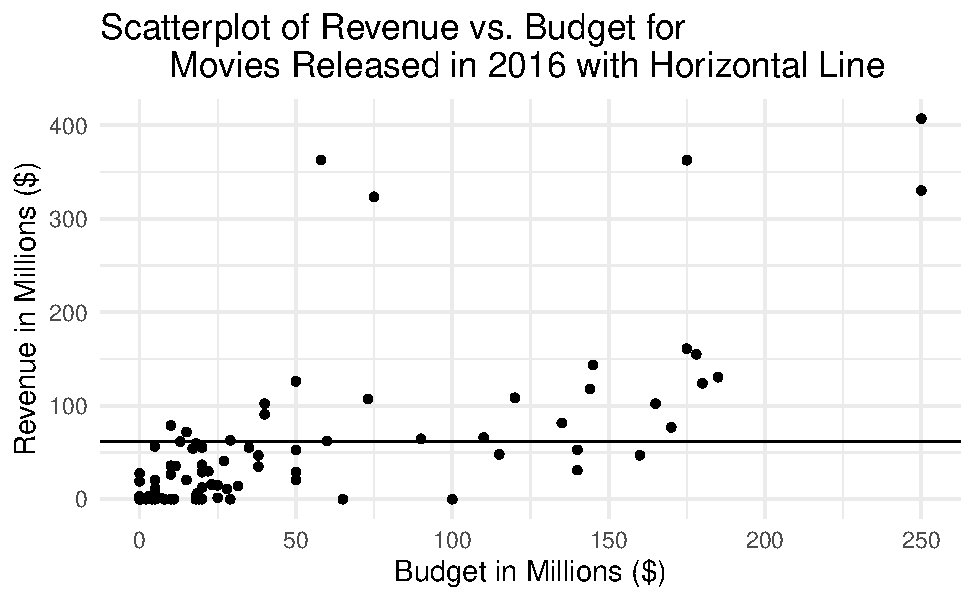
\includegraphics[width=0.7\linewidth]{04-OCA03-EDA-two-quantitative-corr_files/figure-latex/unnamed-chunk-2-1} \end{center}

The calculated value for the SST is 730207.72.

This next scatterplot, shows the plotted data with the best fit regression line. We will learn more about the regression line in the next class. This is the line of best fit between budget and revenue and has the smallest sum of squares error (SSE). The SSE is calculated by finding the residual from each response value to the regression line. Each residual is squared and the sum of the squared values is calculated.

\begin{center}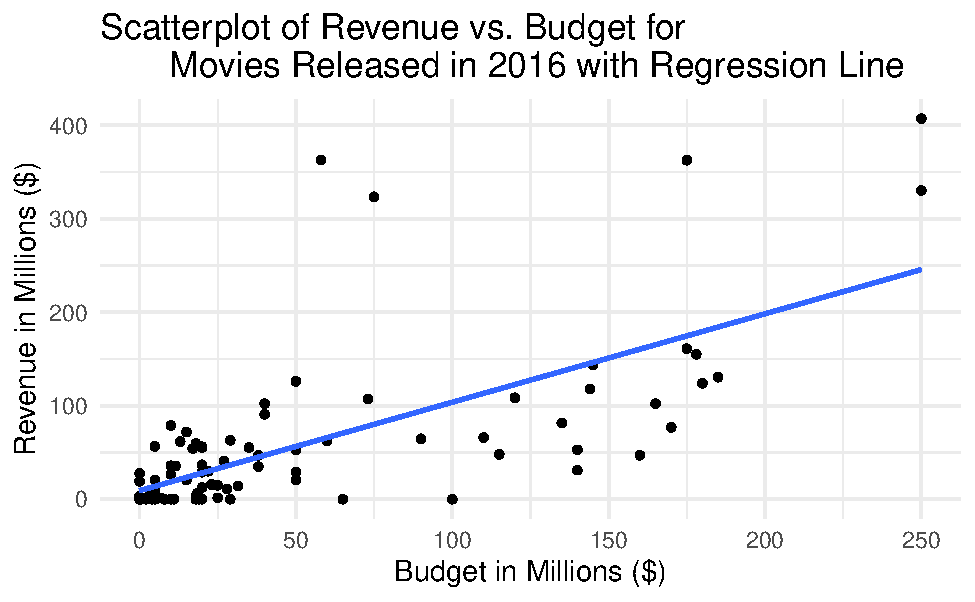
\includegraphics[width=0.7\linewidth]{04-OCA03-EDA-two-quantitative-corr_files/figure-latex/unnamed-chunk-3-1} \end{center}

The calculated value for the SSE is 386279.71.

\begin{enumerate}
\def\labelenumi{\arabic{enumi}.}
\setcounter{enumi}{5}
\tightlist
\item
  Calculate the value for \(r^2\) using the values for SST and SSE provided below each of the previous graphs.
\end{enumerate}

\vspace{1in}

\begin{enumerate}
\def\labelenumi{\arabic{enumi}.}
\setcounter{enumi}{6}
\tightlist
\item
  Write a sentence interpreting the coefficient of determination in context of the problem.
\end{enumerate}

\newpage

\hypertarget{take-home-messages-6}{%
\subsection{Take-home messages}\label{take-home-messages-6}}

\begin{enumerate}
\def\labelenumi{\arabic{enumi}.}
\item
  The sign of correlation and the sign of the slope will always be the same. The closer the value of correlation is to \(-1\) or \(+1\), the stronger the linear relationship between the explanatory and the response variable.
\item
  The coefficient of determination multiplied by 100 (\(r^2 \times 100\)) measures the percent of variation in the response variable that is explained by the relationship with the explanatory variable. The closer the value of the coefficient of determination is to 100\%, the stronger the relationship.
\end{enumerate}

\hypertarget{additional-notes-6}{%
\subsection{Additional notes}\label{additional-notes-6}}

Use this space to summarize your thoughts and take additional notes on today's activity and material covered.

\newpage

\hypertarget{activity-4-movie-profits-linear-regression}{%
\section{Activity 4: Movie Profits --- Linear Regression}\label{activity-4-movie-profits-linear-regression}}

\setstretch{1}

\hypertarget{learning-outcomes-8}{%
\subsection{Learning outcomes}\label{learning-outcomes-8}}

\begin{itemize}
\item
  Identify and create appropriate summary statistics and plots
  given a data set with two quantitative variables.
\item
  Use scatterplots to assess the relationship between two quantitative variables.
\item
  Find the estimated line of regression using summary statistics and \texttt{R} linear model (\texttt{lm()}) output.
\item
  Interpret the slope coefficient in context of the problem.
\end{itemize}

\hypertarget{terminology-review-8}{%
\subsection{Terminology review}\label{terminology-review-8}}

In today's activity, we will review summary measures and plots for two quantitative variables. Some terms covered in this activity are:

\begin{itemize}
\item
  Scatterplot
\item
  Least-squares line of regression
\item
  Slope and \(y\)-intercept
\item
  Residuals
\end{itemize}

To review these concepts, see Chapter 6 \& 7 in the textbook.

\hypertarget{movies-released-in-2016-2}{%
\subsection{Movies released in 2016}\label{movies-released-in-2016-2}}

We will revisit the movie data set collected on Movies released in 2016 ({``{IMDb} Movies Extensive Dataset''} 2016) to further explore the relationship between budget and revenue. Here is a reminder of the variables collected on these movies. (Note: both budget and revenue are measured in ``millions of dollars'' (\$MM).)

\begin{longtable}[]{@{}
  >{\raggedright\arraybackslash}p{(\columnwidth - 2\tabcolsep) * \real{0.2353}}
  >{\raggedright\arraybackslash}p{(\columnwidth - 2\tabcolsep) * \real{0.7647}}@{}}
\toprule\noalign{}
\begin{minipage}[b]{\linewidth}\raggedright
\textbf{Variable}
\end{minipage} & \begin{minipage}[b]{\linewidth}\raggedright
\textbf{Description}
\end{minipage} \\
\midrule\noalign{}
\endhead
\bottomrule\noalign{}
\endlastfoot
\texttt{budget\_mil} & Amount of money (\$MM) budgeted for the production of the movie \\
\texttt{revenue\_mil} & Amount of money (\$MM) the movie made after release \\
\texttt{duration} & Length of the movie (in minutes) \\
\texttt{content\_rating} & Rating of the movie (\texttt{G}, \texttt{PG}, \texttt{PG-13}, \texttt{R}, \texttt{Not\ Rated}) \\
\texttt{imdb\_score} & IMDb user rating score from 1 to 10 \\
\texttt{genres} & Categories the movie falls into (e.g., Action, Drama, etc.) \\
\texttt{facebook\_likes} & Number of likes a movie receives on Facebook \\
\end{longtable}

\begin{Shaded}
\begin{Highlighting}[]
\NormalTok{movies }\OtherTok{\textless{}{-}} \FunctionTok{read.csv}\NormalTok{(}\StringTok{"https://math.montana.edu/courses/s216/data/Movies2016.csv"}\NormalTok{) }\CommentTok{\# Reads in data set }
\end{Highlighting}
\end{Shaded}

\hypertarget{vocabulary-review}{%
\subsubsection*{Vocabulary review}\label{vocabulary-review}}
\addcontentsline{toc}{subsubsection}{Vocabulary review}

To look at the relationship between two quantitative variables we will create a scatterplot with the explanatory variable on the x-axis and the response variable on the y-axis.

We will look at the relationship between budget and revenue for movies released in 2016.

\begin{itemize}
\item
  Upload and open the provided R script file.
\item
  Enter the explanatory variable name, \texttt{budget\_mil}, for \texttt{explanatory} and the response variable name, \texttt{revenue\_mil}, for \texttt{response} at line 9 in the R script file to create the scatterplot.
\item
  Highlight and run lines 1--14.
\end{itemize}

\begin{Shaded}
\begin{Highlighting}[]
\NormalTok{movies }\SpecialCharTok{\%\textgreater{}\%} \CommentTok{\# Data set pipes into...}
\FunctionTok{ggplot}\NormalTok{(}\FunctionTok{aes}\NormalTok{(}\AttributeTok{x =}\NormalTok{ explanatory, }\AttributeTok{y =}\NormalTok{ response))}\SpecialCharTok{+}  \CommentTok{\# Specify variables}
  \FunctionTok{geom\_point}\NormalTok{() }\SpecialCharTok{+}  \CommentTok{\# Add scatterplot of points}
  \FunctionTok{labs}\NormalTok{(}\AttributeTok{x =} \StringTok{"Budget in Millions ($)"}\NormalTok{,  }\CommentTok{\# Label x{-}axis}
       \AttributeTok{y =} \StringTok{"Revenue in Millions ($)"}\NormalTok{,  }\CommentTok{\# Label y{-}axis}
       \AttributeTok{title =} \StringTok{"Scatterplot of Revenue vs. Budget for Movies }
\StringTok{       Released in 2016"}\NormalTok{) }\SpecialCharTok{+} 
    \CommentTok{\# Be sure to title your plots}
  \FunctionTok{geom\_smooth}\NormalTok{(}\AttributeTok{method =} \StringTok{"lm"}\NormalTok{, }\AttributeTok{se =} \ConstantTok{FALSE}\NormalTok{)  }\CommentTok{\# Add regression line}
\end{Highlighting}
\end{Shaded}

\begin{enumerate}
\def\labelenumi{\arabic{enumi}.}
\tightlist
\item
  Sketch the scatterplot created from the code.
\end{enumerate}

\vspace{1.75in}

\begin{enumerate}
\def\labelenumi{\arabic{enumi}.}
\setcounter{enumi}{1}
\tightlist
\item
  Assess the four features of the scatterplot that describe this relationship.
\end{enumerate}

\begin{itemize}
\tightlist
\item
  Form (linear, non-linear)
\end{itemize}

\vspace{.075in}

\begin{itemize}
\tightlist
\item
  Direction (positive, negative)
\end{itemize}

\vspace{.075in}

\begin{itemize}
\tightlist
\item
  Strength
\end{itemize}

\vspace{.075in}

\begin{itemize}
\tightlist
\item
  Unusual observations or outliers
\end{itemize}

\vspace{.075in}

\begin{enumerate}
\def\labelenumi{\arabic{enumi}.}
\setcounter{enumi}{2}
\tightlist
\item
  Based on the plot, does there appear to be an association between budget and revenue? Explain.
\end{enumerate}

\vspace{1in}

\hypertarget{slope}{%
\subsubsection*{Slope}\label{slope}}
\addcontentsline{toc}{subsubsection}{Slope}

The linear model function in R (\texttt{lm()}) gives us the summary for the least squares regression line. The estimate for \texttt{(Intercept)} is the \(y\)-intercept for the line of least squares, and the estimate for \texttt{budget\_mil} (the \(x\)-variable name) is the value of \(b_1\), the slope.

\begin{itemize}
\tightlist
\item
  Run lines 18--19 in the R script file to reproduce the linear model output found in the coursepack.
\end{itemize}

\begin{Shaded}
\begin{Highlighting}[]
\CommentTok{\# Fit linear model: y \textasciitilde{} x}
\NormalTok{revenueLM }\OtherTok{\textless{}{-}} \FunctionTok{lm}\NormalTok{(revenue\_mil }\SpecialCharTok{\textasciitilde{}}\NormalTok{ budget\_mil, }\AttributeTok{data=}\NormalTok{movies)}
\FunctionTok{summary}\NormalTok{(revenueLM)}\SpecialCharTok{$}\NormalTok{coefficients }\CommentTok{\# Display coefficient summary}
\end{Highlighting}
\end{Shaded}

\begin{verbatim}
#>              Estimate Std. Error  t value     Pr(>|t|)
#> (Intercept) 9.1693054  9.0175499 1.016829 3.119606e-01
#> budget_mil  0.9460001  0.1056786 8.951670 4.339561e-14
\end{verbatim}

\begin{enumerate}
\def\labelenumi{\arabic{enumi}.}
\setcounter{enumi}{3}
\tightlist
\item
  Write out the least squares regression line using the summary statistics provided above in context of the problem.
  \vspace{0.8in}
\end{enumerate}

You may remember from middle and high school that slope \(=\frac{\mbox{rise}}{\mbox{run}}\).

Using \(b_1\) to represent slope, we can write that as the fraction \(\frac{b_1}{1}\).

Therefore, the slope predicts how much the line will \emph{rise} for each \emph{run} of +1. In other words, as the \(x\) variable increases by 1 unit, the \(y\) variable is predicted to change (increase/decrease) by the value of slope.

\begin{enumerate}
\def\labelenumi{\arabic{enumi}.}
\setcounter{enumi}{4}
\tightlist
\item
  Interpret the value of slope in context of the problem.
\end{enumerate}

\vspace{.8in}

\begin{enumerate}
\def\labelenumi{\arabic{enumi}.}
\setcounter{enumi}{5}
\tightlist
\item
  Using the least squares line from question 4, predict the revenue for a movie with a budget of 165 \$MM.
\end{enumerate}

\vspace{.6in}

\begin{enumerate}
\def\labelenumi{\arabic{enumi}.}
\setcounter{enumi}{6}
\tightlist
\item
  Predict the revenue for a movie with a budget of 500 \$MM.
\end{enumerate}

\vspace{0.8in}

\begin{enumerate}
\def\labelenumi{\arabic{enumi}.}
\setcounter{enumi}{7}
\tightlist
\item
  The prediction in question 7 is an example of what?
\end{enumerate}

\vspace{0.3in}

\hypertarget{residuals}{%
\subsubsection*{Residuals}\label{residuals}}
\addcontentsline{toc}{subsubsection}{Residuals}

The model we are using assumes the relationship between the two variables follows a straight line. The residuals are the errors, or the variability in the response that hasn't been modeled by the regression line.

\begin{center}

$\implies$ Residual = actual y value $-$ predicted y value

$e=y-\hat{y}$
\end{center}

\begin{enumerate}
\def\labelenumi{\arabic{enumi}.}
\setcounter{enumi}{8}
\tightlist
\item
  The movie \emph{Independence Day: Resurgence} had a budget of 165 \$MM and revenue of 102.315 \$MM. Find the residual for this movie.
\end{enumerate}

\vspace{.8in}

\begin{enumerate}
\def\labelenumi{\arabic{enumi}.}
\setcounter{enumi}{9}
\tightlist
\item
  Did the line of regression overestimate or underestimate the revenue for this movie?
\end{enumerate}

\vspace{.2in}

\hypertarget{multivariable-plots-1}{%
\subsubsection*{Multivariable plots}\label{multivariable-plots-1}}
\addcontentsline{toc}{subsubsection}{Multivariable plots}

What if we wanted to see if the relationship between movie budget and revenue differs if we add another variable into the picture? The following plot visualizes three variables, creating a \textbf{multivariable} plot.

\begin{Shaded}
\begin{Highlighting}[]
\NormalTok{movies }\SpecialCharTok{\%\textgreater{}\%} \CommentTok{\# Data set pipes into...}
  \FunctionTok{filter}\NormalTok{(content\_rating }\SpecialCharTok{!=} \StringTok{"Not Rated"}\NormalTok{) }\SpecialCharTok{\%\textgreater{}\%} \CommentTok{\# Remove Not Rated movies}
  \FunctionTok{ggplot}\NormalTok{(}\FunctionTok{aes}\NormalTok{(}\AttributeTok{x =}\NormalTok{ budget\_mil, }\AttributeTok{y =}\NormalTok{ revenue\_mil, }\AttributeTok{color =}\NormalTok{ content\_rating)) }\SpecialCharTok{+}  \CommentTok{\# Specify variables}
  \FunctionTok{geom\_point}\NormalTok{(}\FunctionTok{aes}\NormalTok{(}\AttributeTok{shape =}\NormalTok{ content\_rating), }\AttributeTok{size =} \DecValTok{2}\NormalTok{) }\SpecialCharTok{+}  \CommentTok{\# Add scatterplot of points}
  \FunctionTok{labs}\NormalTok{(}\AttributeTok{x =} \StringTok{"Budget in Millions ($)"}\NormalTok{,  }\CommentTok{\# Label x{-}axis}
       \AttributeTok{y =} \StringTok{"Revenue in Millions ($)"}\NormalTok{,  }\CommentTok{\# Label y{-}axis}
       \AttributeTok{color =} \StringTok{"content\_rating"}\NormalTok{,  }\CommentTok{\# Label legend}
       \AttributeTok{title =} \StringTok{"Scatterplot of Revenue vs. Budget by }
\StringTok{       Content Rating for Movies Released in 2016"}\NormalTok{) }\SpecialCharTok{+} 
    \CommentTok{\# Be sure to title your plot}
  \FunctionTok{geom\_smooth}\NormalTok{(}\AttributeTok{method =} \StringTok{"lm"}\NormalTok{, }\AttributeTok{se =} \ConstantTok{FALSE}\NormalTok{, }\AttributeTok{lwd =} \DecValTok{2}\NormalTok{) }\SpecialCharTok{+} \CommentTok{\# Add regression lines}
  \FunctionTok{scale\_color\_grey}\NormalTok{() }\CommentTok{\# Make black and white}
\end{Highlighting}
\end{Shaded}

\begin{center}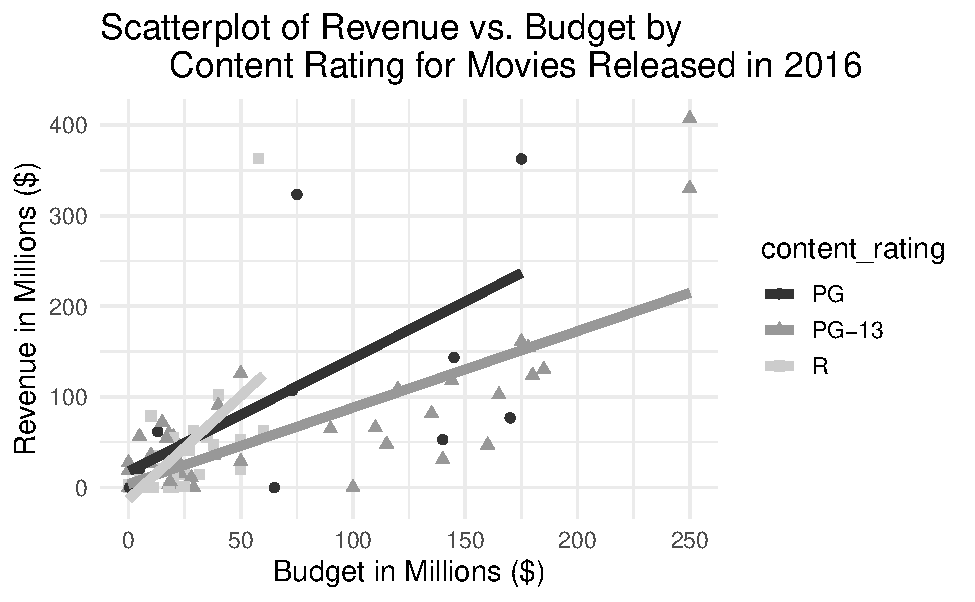
\includegraphics[width=0.7\linewidth]{04-A04-EDA-two-quantitative-LR_files/figure-latex/unnamed-chunk-4-1} \end{center}

\begin{enumerate}
\def\labelenumi{\arabic{enumi}.}
\setcounter{enumi}{10}
\tightlist
\item
  Identify the three variables plotted in this graph.
\end{enumerate}

\vspace{0.5in}

\begin{enumerate}
\def\labelenumi{\arabic{enumi}.}
\setcounter{enumi}{11}
\tightlist
\item
  Does the \emph{relationship} between movie budget and revenue differ among the different content ratings? Explain.
\end{enumerate}

\vspace{0.8in}
\newpage

\hypertarget{take-home-messages-7}{%
\subsection{Take-home messages}\label{take-home-messages-7}}

\begin{enumerate}
\def\labelenumi{\arabic{enumi}.}
\item
  Two quantitative variables are graphically displayed in a scatterplot. The explanatory variable is on the \(x\)-axis and the response variable is on the \(y\)-axis. When describing the relationship between two quantitative variables we look at the form (linear or non-linear), direction (positive or negative), strength, and for the presence of outliers.
\item
  There are three summary statistics used to summarize the relationship between two quantitative variables: correlation (\(r\)), slope of the regression line (\(b_1\)), and the coefficient of determination (\(r^2\)).
\item
  We can use the line of regression to predict values of the response variable for values of the explanatory variable. Do not use values of the explanatory variable that are outside of the range of values in the data set to predict values of the response variable (reflect on why this is true.). This is called \textbf{extrapolation}.
\end{enumerate}

\hypertarget{additional-notes-7}{%
\subsection{Additional notes}\label{additional-notes-7}}

Use this space to summarize your thoughts and take additional notes on today's activity and material covered.

\newpage

\hypertarget{week-4-lab-penguins}{%
\section{Week 4 Lab: Penguins}\label{week-4-lab-penguins}}

\setstretch{1}

\hypertarget{learning-outcomes-9}{%
\subsection{Learning outcomes}\label{learning-outcomes-9}}

\begin{itemize}
\item
  Identify and create appropriate summary statistics and plots
  given a data set with two quantitative variables.
\item
  Use scatterplots to assess the relationship between two quantitative variables.
\item
  Find the estimated line of regression using summary statistics and R linear model (\texttt{lm()}) output.
\item
  Interpret the slope coefficient in context of the problem.
\item
  Calculate and interpret \(r^2\), the coefficient of determination, in context of the problem.
\item
  Find the correlation coefficient from R output or from \(r^2\) and the sign of the slope.
\end{itemize}

\hypertarget{penguins}{%
\subsection*{Penguins}\label{penguins}}
\addcontentsline{toc}{subsection}{Penguins}

The Palmer Station Long Term Ecological Research Program sampled three penguin species on islands in the Palmer Archipelago in Antarctica. Researchers took various body measurements on the penguins, including bill depth and body mass. The researchers were interested in the relationship between bill depth and body mass and wondered if bill depth could be used to accurately predict the body mass of these three penguin species.

\begin{itemize}
\item
  Upload and import the \texttt{Antarctica\_Penguins} csv file
\item
  Upload and open the provided R script file for week 4 lab.
\item
  Enter the name of the data set (see the environment tab) for \texttt{datasetname} in the R script file in line 5.
\end{itemize}

First we will create a scatterplot of the bill depth and body mass. Notice that we are using bill depth (mm) to predict body mass (g). This makes bill depth the explanatory variable.

\begin{itemize}
\item
  \textbf{Make sure to give your plot a descriptive title between the quotations in line 16. Remember that the title should include the type of plot, the observational units, and the variable(s) plotted.}
\item
  Highlight and run lines 1--17 in the R script file.
\item
  \textbf{Upload a copy of your scatterplot to Gradescope.}
\end{itemize}

\begin{Shaded}
\begin{Highlighting}[]
\NormalTok{penguins }\OtherTok{\textless{}{-}}\NormalTok{ datasetname }\SpecialCharTok{\%\textgreater{}\%} \CommentTok{\#Creates the object penguins}
    \FunctionTok{na.omit}\NormalTok{() }\CommentTok{\#Removes data points without values}
\NormalTok{penguins }\SpecialCharTok{\%\textgreater{}\%}
  \FunctionTok{ggplot}\NormalTok{(}\FunctionTok{aes}\NormalTok{(}\AttributeTok{x =}\NormalTok{ bill\_depth\_mm, }\AttributeTok{y =}\NormalTok{ body\_mass\_g))}\SpecialCharTok{+}  \CommentTok{\# Specify variables}
  \FunctionTok{geom\_point}\NormalTok{(}\AttributeTok{alpha=}\FloatTok{0.5}\NormalTok{) }\SpecialCharTok{+}  \CommentTok{\# Add scatterplot of points}
  \FunctionTok{labs}\NormalTok{(}\AttributeTok{x =} \StringTok{"bill depth (mm)"}\NormalTok{,  }\CommentTok{\# Label x{-}axis}
       \AttributeTok{y =} \StringTok{"body mass (g)"}\NormalTok{,  }\CommentTok{\# Label y{-}axis}
       \AttributeTok{title =} \StringTok{"Title"}\NormalTok{) }\SpecialCharTok{+} \CommentTok{\# Be sure to title your plot}
  \FunctionTok{geom\_smooth}\NormalTok{(}\AttributeTok{method =} \StringTok{"lm"}\NormalTok{, }\AttributeTok{se =} \ConstantTok{FALSE}\NormalTok{)  }\CommentTok{\# Add regression line}
\end{Highlighting}
\end{Shaded}

\newpage

\begin{enumerate}
\def\labelenumi{\arabic{enumi}.}
\tightlist
\item
  Assess the four features of the scatterplot that describe this relationship.
  \vspace{1mm}
\end{enumerate}

\begin{itemize}
\tightlist
\item
  Form (linear, non-linear)
\end{itemize}

\vspace{.1in}

\begin{itemize}
\tightlist
\item
  Direction (positive, negative)
\end{itemize}

\vspace{.1in}

\begin{itemize}
\tightlist
\item
  Strength
\end{itemize}

\vspace{.1in}

\begin{itemize}
\tightlist
\item
  Unusual observations or outliers
\end{itemize}

\vspace{.1in}

To create the correlation matrix\ldots{}

\begin{itemize}
\tightlist
\item
  Highlight and run lines 20--24 in the R script file.
\end{itemize}

\begin{Shaded}
\begin{Highlighting}[]
\NormalTok{penguins }\SpecialCharTok{\%\textgreater{}\%}  \CommentTok{\# Data set pipes into}
  \FunctionTok{select}\NormalTok{(}\FunctionTok{c}\NormalTok{(}\StringTok{"bill\_length\_mm"}\NormalTok{, }\StringTok{"bill\_depth\_mm"}\NormalTok{, }
           \StringTok{"flipper\_length\_mm"}\NormalTok{, }\StringTok{"body\_mass\_g"}\NormalTok{)) }\SpecialCharTok{\%\textgreater{}\%}
  \FunctionTok{cor}\NormalTok{(}\AttributeTok{use=}\StringTok{"pairwise.complete.obs"}\NormalTok{) }\SpecialCharTok{\%\textgreater{}\%}
  \FunctionTok{round}\NormalTok{(}\DecValTok{3}\NormalTok{)}
\end{Highlighting}
\end{Shaded}

\begin{enumerate}
\def\labelenumi{\arabic{enumi}.}
\setcounter{enumi}{1}
\tightlist
\item
  Using the R output, report the value of correlation between bill depth and body mass.
\end{enumerate}

\vspace{0.5in}

\begin{enumerate}
\def\labelenumi{\arabic{enumi}.}
\setcounter{enumi}{2}
\tightlist
\item
  Using the value of correlation found in question 2, calculate the value of the coefficient of determination.
\end{enumerate}

\vspace{0.5in}

\begin{enumerate}
\def\labelenumi{\arabic{enumi}.}
\setcounter{enumi}{3}
\tightlist
\item
  \textbf{Interpret the coefficient of determination in context of the problem.}
\end{enumerate}

\vspace{0.8in}

To get the linear model output\ldots{}

\begin{itemize}
\item
  Enter the variable name \texttt{body\_mass\_g} for \texttt{response} and the variable name \texttt{bill\_depth\_mm} for \texttt{explanatory} in line 29 in the R script file.
\item
  Highlight and run lines 29--30.
\end{itemize}

\begin{Shaded}
\begin{Highlighting}[]
\CommentTok{\# Fit linear model: y \textasciitilde{} x}
\NormalTok{penguinsLM }\OtherTok{\textless{}{-}} \FunctionTok{lm}\NormalTok{(response}\SpecialCharTok{\textasciitilde{}}\NormalTok{explanatory, }\AttributeTok{data=}\NormalTok{penguins)}
\FunctionTok{summary}\NormalTok{(penguinsLM)}\SpecialCharTok{$}\NormalTok{coefficients }\CommentTok{\# Display coefficient summary}
\end{Highlighting}
\end{Shaded}

\begin{enumerate}
\def\labelenumi{\arabic{enumi}.}
\setcounter{enumi}{4}
\tightlist
\item
  Write out the least squares regression line using the summary statistics from the R output in context of the problem.
\end{enumerate}

\vspace{.5in}

\begin{enumerate}
\def\labelenumi{\arabic{enumi}.}
\setcounter{enumi}{5}
\tightlist
\item
  \textbf{Interpret the value of slope in context of the problem.}
\end{enumerate}

\vspace{.8in}

\begin{enumerate}
\def\labelenumi{\arabic{enumi}.}
\setcounter{enumi}{6}
\tightlist
\item
  \textbf{Using the least squares regression line from question 5, predict the body mass for a penguin with a bill depth of 19.6 mm.}
\end{enumerate}

\vspace{.6in}

\begin{enumerate}
\def\labelenumi{\arabic{enumi}.}
\setcounter{enumi}{7}
\tightlist
\item
  One penguin had a bill depth of 19.6 mm and a body mass of 4675 g. Find the residual for this penguin.
\end{enumerate}

\vspace{.8in}

\begin{enumerate}
\def\labelenumi{\arabic{enumi}.}
\setcounter{enumi}{8}
\tightlist
\item
  Did the line of regression overestimate or underestimate the body mass for this penguin?
\end{enumerate}

\vspace{0.2in}

Does species change the relationship between bill depth and body mass?

\begin{itemize}
\tightlist
\item
  Highlight and run lines 34 - 43 to get the multivariable plot.
\end{itemize}

\begin{Shaded}
\begin{Highlighting}[]
\NormalTok{penguins }\SpecialCharTok{\%\textgreater{}\%}
  \FunctionTok{ggplot}\NormalTok{(}\FunctionTok{aes}\NormalTok{(}\AttributeTok{x =}\NormalTok{ bill\_depth\_mm, }\AttributeTok{y =}\NormalTok{ body\_mass\_g, }\AttributeTok{color=}\NormalTok{species))}\SpecialCharTok{+}  \CommentTok{\# Specify variables}
  \FunctionTok{geom\_point}\NormalTok{(}\FunctionTok{aes}\NormalTok{(}\AttributeTok{shape =}\NormalTok{ species), }\AttributeTok{size =} \DecValTok{2}\NormalTok{, }\AttributeTok{alpha=}\FloatTok{0.5}\NormalTok{) }\SpecialCharTok{+}  \CommentTok{\# Add scatterplot of points}
  \FunctionTok{labs}\NormalTok{(}\AttributeTok{x =} \StringTok{"bill depth (mm)"}\NormalTok{,  }\CommentTok{\# Label x{-}axis}
       \AttributeTok{y =} \StringTok{"body mass (g)"}\NormalTok{,  }\CommentTok{\# Label y{-}axis}
       \AttributeTok{color =} \StringTok{"species"}\NormalTok{,}
       \AttributeTok{shape =} \StringTok{"species"}\NormalTok{,}
       \AttributeTok{title =} \StringTok{"Scatterplot of Bill Depth and Body Mass by Penguin Species"}\NormalTok{) }\SpecialCharTok{+} 
    \CommentTok{\# Enter the title for the plot between the quotations}
  \FunctionTok{geom\_smooth}\NormalTok{(}\AttributeTok{method =} \StringTok{"lm"}\NormalTok{, }\AttributeTok{se =} \ConstantTok{FALSE}\NormalTok{) }\SpecialCharTok{+}  \CommentTok{\# Add regression line}
  \FunctionTok{scale\_color\_viridis\_d}\NormalTok{(}\AttributeTok{end=}\FloatTok{0.8}\NormalTok{)}
\end{Highlighting}
\end{Shaded}

\begin{enumerate}
\def\labelenumi{\arabic{enumi}.}
\setcounter{enumi}{9}
\tightlist
\item
  What three variables are plotted on this plot?
\end{enumerate}

\vspace{0.3in}

\begin{enumerate}
\def\labelenumi{\arabic{enumi}.}
\setcounter{enumi}{10}
\tightlist
\item
  \textbf{Do species and bill depth appear to interact when predicting body mass of Antarctic penguins? Explain your answer.}
\end{enumerate}

\vspace{0.5in}

\begin{enumerate}
\def\labelenumi{\arabic{enumi}.}
\setcounter{enumi}{11}
\tightlist
\item
  Explain the association between species and each of the other two variables.
\end{enumerate}

\vspace{0.5in}

\begin{enumerate}
\def\labelenumi{\arabic{enumi}.}
\setcounter{enumi}{12}
\tightlist
\item
  Notice that the slope of the line between bill depth and body mass for each species is positive while the slope for the line not accounting for species is negative. What phenomena is this an example of?
\end{enumerate}

\vspace{0.2in}

\newpage

\hypertarget{group-exam-1-review}{%
\chapter{Group Exam 1 Review}\label{group-exam-1-review}}

Use the provided data set from the Islands (Bulmer, n.d.) (Exam1ReviewData.csv) and the appropriate Exam 1 Review R script file to answer the following questions. Each adult (\textgreater21) islander was selected at random from all adult islanders. Note that some islanders choose not to participate in the study. These islanders that did not consent to be in the study are removed from the dataset before analysis. Variables and their descriptions are listed below. Here is some more information about some of the variables collected. Music type (classical or heavy metal) was randomly assigned to the Islanders. Time to complete the puzzle cube was measured after listening to music for each Islander. Heart rate and blood glucose levels were both measured before and then after drinking a caffeinated beverage.

\begin{longtable}[]{@{}
  >{\raggedright\arraybackslash}p{(\columnwidth - 2\tabcolsep) * \real{0.2353}}
  >{\raggedright\arraybackslash}p{(\columnwidth - 2\tabcolsep) * \real{0.7647}}@{}}
\toprule\noalign{}
\begin{minipage}[b]{\linewidth}\raggedright
\textbf{Variable}
\end{minipage} & \begin{minipage}[b]{\linewidth}\raggedright
\textbf{Description}
\end{minipage} \\
\midrule\noalign{}
\endhead
\bottomrule\noalign{}
\endlastfoot
\texttt{Island} & Name of Island that the Islander resides on \\
\texttt{City} & Name of City in which the Islander resides \\
\texttt{Population} & Population of the City \\
\texttt{Name} & Name of Islander \\
\texttt{Consent} & Whether the Islander consented to be in the study (\texttt{Declined}, \texttt{Consented}) \\
\texttt{Gender} & Gender of Islander (\texttt{M} = male, \texttt{F} = Female) \\
\texttt{Age} & Age of Islander \\
\texttt{Married} & Marital status of Islander (\texttt{yes}, \texttt{no}) \\
\texttt{Smoking\_Status} & Whether the Islander is a current smoker (\texttt{nonsmoker}, \texttt{smoker}) \\
\texttt{Children} & Whether the Islander has children (\texttt{yes}, \texttt{no}) \\
\texttt{weight\_kg} & Weight measured in kg \\
\texttt{height\_cm} & Height measured in cm \\
\texttt{respiratory\_rate} & Breaths per minute \\
\texttt{Type\_of\_Music} & Music type Islander was randomly assigned to listen to (\texttt{Classical}, \texttt{Heavy\ Metal}) \\
\texttt{After\_PuzzleCube} & Time to complete puzzle cube (minutes) after listening to assigned music \\
\texttt{Education\_Level} & Highest level of education completed (\texttt{highschool}, \texttt{university}) \\
\texttt{Balance\_Test} & Time balanced measured in seconds with eyes closed \\
\texttt{Blood\_Glucose\_before} & Level of blood glucose (mg/dL) before consuming assigned drink \\
\texttt{Heart\_Rate\_before} & Heart rate (bpm) before consuming assigned drink \\
\texttt{Blood\_Glucose\_after} & Level of blood glucose (mg/dL) after consuming assigned drink \\
\texttt{Heart\_Rate\_after} & Heart rate (bpm) after consuming assigned drink \\
\texttt{Diff\_Heart\_Rate} & Difference in heart rate (bpm) for Before - After consuming assigned drink \\
\texttt{Diff\_Blood\_Glucose} & Difference in blood glucose (mg/dL) for Before - After consuming assigned drink \\
\end{longtable}

\begin{enumerate}
\def\labelenumi{\arabic{enumi}.}
\tightlist
\item
  What are the observational units?
\end{enumerate}

\vspace{0.1in}

\begin{enumerate}
\def\labelenumi{\arabic{enumi}.}
\setcounter{enumi}{1}
\tightlist
\item
  In the table above, indicate which variables are categorical (C) and which variables are quantitative (Q).
\end{enumerate}

\vspace{0.1in}

\begin{enumerate}
\def\labelenumi{\arabic{enumi}.}
\setcounter{enumi}{2}
\tightlist
\item
  What type of bias may be present in this study? Explain.
\end{enumerate}

\vspace{0.5in}

\newpage

\textbf{Complete questions 4a, 4b, 5a, 5b, 6a, and 6b. Then choose the scenario for each research question and use the appropriate Exam 1 Review R script file to find the summary statistic(s) and graphical display of the research question.}

\begin{enumerate}
\def\labelenumi{\arabic{enumi}.}
\setcounter{enumi}{3}
\tightlist
\item
  Use the appropriate Exam 1 Review R script file to find the summary statistic and graphical display of the data to assess the following research question, ``Is there a difference in proportion of Islanders who have children for those who completed high school and those that completed university?'' Use high school \(-\) university as the order of subtraction.
\end{enumerate}

\begin{enumerate}
\def\labelenumi{\alph{enumi}.}
\item
  What is the name of the explanatory variable to be assessed in this research question?
  \vspace{0.3in}

  What type of variable (categorical or quantitative) is the variable you identified?
  \vspace{0.3in}
\item
  What is the name of the response variable to be assessed in this research question?
  \vspace{0.3in}

  What type of variable (categorical or quantitative) is the variable you identified?
  \vspace{0.3in}
\item
  Use the R script file to get the counts for each level and combination of variables. Fill in the following table with the variable names, levels of each variable, and counts using the values from the R output.
\end{enumerate}

\begingroup
\setlength{\tabcolsep}{14pt}
\renewcommand{\arraystretch}{2}
\begin{center}
\begin{tabular}{|c|p{1in}|p{1in}|p{1in}|}
\hline
 & \multicolumn{2}{|c|}{\textbf{Explanatory Variable}} & \\ 
 & \multicolumn{2}{|c|}{ } & \\ \hline
\textbf{Response variable} & Group 1 & Group 2 & Total \\
 & & & \\ \hline
 Success & & & \\
 & & & \\ \hline
 Failure & & & \\
 & & & \\ \hline
 Total & & & \\
 & & & \\ \hline
\end{tabular}
\end{center}
\endgroup

\begin{enumerate}
\def\labelenumi{\alph{enumi}.}
\setcounter{enumi}{3}
\tightlist
\item
  Calculate the value of the summary statistic to answer the research question. Give appropriate notation.
\end{enumerate}

\newpage

\begin{enumerate}
\def\labelenumi{\alph{enumi}.}
\setcounter{enumi}{4}
\item
  Interpret the value of the summary statistic in context of the problem:
  \vspace{0.5in}
\item
  What type of graph(s) would be appropriate for this research question?
\end{enumerate}

\vspace{0.2in}

\begin{enumerate}
\def\labelenumi{\alph{enumi}.}
\setcounter{enumi}{6}
\tightlist
\item
  Using the provided R file create a graph of the data. Sketch the graph below:
\end{enumerate}

\vspace{2in}

\begin{enumerate}
\def\labelenumi{\alph{enumi}.}
\setcounter{enumi}{7}
\tightlist
\item
  Does there appear to be an association between the two variables? Clearly explain your answer using the graph and calculated summary statistic.
\end{enumerate}

\vspace{0.8in}

\begin{enumerate}
\def\labelenumi{\roman{enumi}.}
\tightlist
\item
  Is this an observational study or a randomized experiment? Explain your answer.
\end{enumerate}

\vspace{0.5in}

\begin{enumerate}
\def\labelenumi{\alph{enumi}.}
\setcounter{enumi}{9}
\tightlist
\item
  What is the scope of inference for this study?
\end{enumerate}

\newpage

\begin{enumerate}
\def\labelenumi{\arabic{enumi}.}
\setcounter{enumi}{4}
\tightlist
\item
  Use the appropriate Exam 1 Review R script file to find the appropriate summary statistic and graphical display of the data to assess the following research question: ``Do Islanders who listen to classical music take less time to complete the puzzle cube after listening to the music than for Islanders that listen to heavy metal music?'' Use classical \(-\) heavy metal as the order of subtraction.
\end{enumerate}

\begin{enumerate}
\def\labelenumi{\alph{enumi}.}
\item
  What is the name of the explanatory variable to be assessed in this research question?
  \vspace{0.3in}

  What type of variable (categorical or quantitative) is the variable you identified?
  \vspace{0.3in}
\item
  What is the name of the response variable to be assessed in this research question?
  \vspace{0.3in}

  What type of variable (categorical or quantitative) is the variable you identified?
  \vspace{0.3in}
\item
  Use the R script file to get the summary statistics for each level of the explanatory variable. Fill in the following table with the variable name, levels of the variable, and the summary statistics from the R output.
\end{enumerate}

\begingroup
\setlength{\tabcolsep}{14pt}
\renewcommand{\arraystretch}{2}
\begin{center}
\begin{tabular}{|c|p{1in}|p{1in}|}
\hline
 & \multicolumn{2}{|c|}{\textbf{Explanatory Variable}} \\
 & \multicolumn{2}{|c|}{ } \\ \hline
\textbf{Summary value} & Group 1 & Group 2 \\
 & & \\ \hline
 Mean & & \\ \hline
 Standard deviation & & \\ \hline
 Sample size & & \\ \hline
\end{tabular}
\end{center}
\endgroup

\begin{enumerate}
\def\labelenumi{\alph{enumi}.}
\setcounter{enumi}{3}
\tightlist
\item
  Calculate the value of the summary statistic to answer the research question. Give appropriate notation.
\end{enumerate}

\vspace{0.4in}

\begin{enumerate}
\def\labelenumi{\alph{enumi}.}
\setcounter{enumi}{4}
\tightlist
\item
  Interpret the value of the summary statistic in context of the problem:
\end{enumerate}

\vspace{0.4in}

\begin{enumerate}
\def\labelenumi{\alph{enumi}.}
\setcounter{enumi}{5}
\tightlist
\item
  What type of graph(s) would be appropriate for this research question?
\end{enumerate}

\vspace{0.2in}

\newpage

\begin{enumerate}
\def\labelenumi{\alph{enumi}.}
\setcounter{enumi}{6}
\tightlist
\item
  Using the provided R file create a graph of the data. Sketch the graph below:
\end{enumerate}

\vspace{2in}

\begin{enumerate}
\def\labelenumi{\alph{enumi}.}
\setcounter{enumi}{7}
\tightlist
\item
  Does there appear to be an association between the two variables? Clearly explain your answer using the graph and calculated summary statistic.
\end{enumerate}

\vspace{0.8in}

\begin{enumerate}
\def\labelenumi{\roman{enumi}.}
\item
  Compare the two plots using the four characteristics to describe plots of quantitative variables.
  \vspace{0.1in}

  Shape:
  \vspace{0.2in}

  Center:
  \vspace{0.2in}

  Spread:
  \vspace{0.2in}

  Outliers:
  \vspace{0.2in}
\end{enumerate}

\begin{enumerate}
\def\labelenumi{\alph{enumi}.}
\setcounter{enumi}{9}
\tightlist
\item
  Is this an observational study or a randomized experiment? Explain your answer.
\end{enumerate}

\vspace{0.5in}

\begin{enumerate}
\def\labelenumi{\alph{enumi}.}
\setcounter{enumi}{10}
\tightlist
\item
  What is the scope of inference for this study?
\end{enumerate}

\newpage

\begin{enumerate}
\def\labelenumi{\arabic{enumi}.}
\setcounter{enumi}{5}
\tightlist
\item
  Use the appropriate Exam 1 Review R script file to find the appropriate summary statistic and graphical display of the data to assess the following research question: ``Do Islanders who are heavier tend to take more breaths per minute?''
\end{enumerate}

\begin{enumerate}
\def\labelenumi{\alph{enumi}.}
\item
  What is the name of the explanatory variable to be assessed in this research question?
  \vspace{0.3in}

  What type of variable (categorical or quantitative) is the variable you identified?
  \vspace{0.3in}
\item
  What is the name of the response variable to be assessed in this research question?
  \vspace{0.3in}

  What type of variable (categorical or quantitative) is the variable you identified?
  \vspace{0.3in}
\item
  Use the R script file to get the summary statistics for this data. Fill in the following table using the values from the R output:
\end{enumerate}

\begingroup
\setlength{\tabcolsep}{14pt}
\renewcommand{\arraystretch}{2}
\begin{center}
\begin{tabular}{|c|p{1in}|p{1in}|p{1in}|}
\hline
 & y-intercept & slope & correlation \\ \hline
 \textbf{Summary value} & & & \\ \hline
\end{tabular}
\end{center}
\endgroup

\begin{enumerate}
\def\labelenumi{\alph{enumi}.}
\setcounter{enumi}{3}
\tightlist
\item
  Interpret the value of slope in context of the problem.
\end{enumerate}

\vspace{0.8in}

\begin{enumerate}
\def\labelenumi{\alph{enumi}.}
\setcounter{enumi}{4}
\tightlist
\item
  Calculate the value of the coefficient of determination.
\end{enumerate}

\vspace{0.3in}

\begin{enumerate}
\def\labelenumi{\alph{enumi}.}
\setcounter{enumi}{5}
\tightlist
\item
  Interpret the coefficient of determination in context of the problem.
\end{enumerate}

\vspace{0.8in}

\begin{enumerate}
\def\labelenumi{\alph{enumi}.}
\setcounter{enumi}{6}
\tightlist
\item
  What type of graph(s) would be appropriate for this research question?
\end{enumerate}

\newpage

\begin{enumerate}
\def\labelenumi{\alph{enumi}.}
\setcounter{enumi}{7}
\tightlist
\item
  Using the provided R file create a graph of the data. Sketch the graph below:
\end{enumerate}

\vspace{2in}

\begin{enumerate}
\def\labelenumi{\roman{enumi}.}
\tightlist
\item
  Does there appear to be an association between the two variables? Clearly explain your answer using the graph and calculated summary statistic.
\end{enumerate}

\vspace{0.8in}

\begin{enumerate}
\def\labelenumi{\alph{enumi}.}
\setcounter{enumi}{9}
\item
  Describe the plot using the four characteristics to describe scatterplots.
  \vspace{0.1in}

  Form:
  \vspace{0.2in}

  Direction:
  \vspace{0.2in}

  Strength:
  \vspace{0.2in}

  Outliers:
  \vspace{0.2in}
\item
  Is this an observational study or a randomized experiment? Explain your answer.
\end{enumerate}

\vspace{0.5in}

\begin{enumerate}
\def\labelenumi{\alph{enumi}.}
\setcounter{enumi}{11}
\tightlist
\item
  What is the scope of inference for this study?
\end{enumerate}

\newpage

\hypertarget{inference-for-a-single-categorical-variable-simulation-based-methods}{%
\chapter{Inference for a Single Categorical Variable: Simulation-based Methods}\label{inference-for-a-single-categorical-variable-simulation-based-methods}}

\hypertarget{lecture-notes-week-6-inference-for-one-categorical-variable-using-simulation-based-methods}{%
\section{Lecture Notes Week 6: Inference for One Categorical Variable using Simulation-based Methods}\label{lecture-notes-week-6-inference-for-one-categorical-variable-using-simulation-based-methods}}

\setstretch{1}

\hypertarget{hypothesis-testing}{%
\subsection*{Hypothesis Testing}\label{hypothesis-testing}}
\addcontentsline{toc}{subsection}{Hypothesis Testing}

Purpose of a hypothesis test:

\begin{itemize}
\item
  Use data collected on a \_\_\_\_\_\_\_\_\_\_\_\_\_\_\_\_\_\_\_\_ to give information about the \_\_\_\_\_\_\_\_\_\_\_\_\_\_\_
\item
  Determines \_\_\_\_\_\_\_\_\_\_\_\_\_\_\_\_\_\_ of \_\_\_\_\_\_\_\_\_\_\_\_\_\_\_\_\_\_\_\_\_ of an effect
\end{itemize}

General steps of a hypothesis test

\begin{enumerate}
\def\labelenumi{\arabic{enumi}.}
\item
  Write a research question and hypotheses.
\item
  Collect data and calculate a summary statistic.
\item
  Model a sampling distribution which assumes the null hypothesis is true.
\item
  Calculate a p-value.
\item
  Draw conclusions based on a p-value.
\end{enumerate}

\hypertarget{hypotheses}{%
\subsection*{Hypotheses}\label{hypotheses}}
\addcontentsline{toc}{subsection}{Hypotheses}

\setstretch{1.5}

\begin{itemize}
\item
  Two possible outcomes:

  \begin{itemize}
  \item
    Either the \_\_\_\_\_\_\_\_\_\_\_\_\_\_\_ hypothesis is true and the \_\_\_\_\_\_\_\_\_\_\_\_\_\_\_\_ occurred by \_\_\_\_\_\_\_\_\_\_\_\_\_\_\_ chance.
  \item
    Or the null hypothesis is \_\_\_\_\_\_\_\_\_\_\_\_\_\_\_ and the sample provides \_\_\_\_\_\_\_\_\_\_\_\_\_\_ against the \_\_\_\_\_\_\_\_\_\_\_\_\_\_.
  \end{itemize}
\item
  Always written about the \_\_\_\_\_\_\_\_\_\_\_\_\_\_\_\_\_\_ (population)
\end{itemize}

\setstretch{1}

\hypertarget{null-hypothesis}{%
\subsubsection*{Null hypothesis}\label{null-hypothesis}}
\addcontentsline{toc}{subsubsection}{Null hypothesis}

\begin{itemize}
\item
  Skeptical perspective, no difference, no effect, random chance
\item
  What the researcher hopes is \_\_\_\_\_\_\_\_\_\_\_\_\_\_\_.
\end{itemize}

Notation:

\vspace{0.2in}

\hypertarget{alternative-hypothesis}{%
\subsubsection*{Alternative hypothesis}\label{alternative-hypothesis}}
\addcontentsline{toc}{subsubsection}{Alternative hypothesis}

\begin{itemize}
\item
  New perspective, a chance, a difference, an effect
\item
  What the researcher hopes is \_\_\_\_\_\_\_\_\_\_\_\_\_\_\_\_.
\end{itemize}

Notation:

\vspace{0.2in}

\hypertarget{simulation-vs.-theory-based-methods}{%
\subsection*{Simulation vs.~Theory-based Methods}\label{simulation-vs.-theory-based-methods}}
\addcontentsline{toc}{subsection}{Simulation vs.~Theory-based Methods}

\hypertarget{simulation-based-method}{%
\subsubsection*{Simulation-based method}\label{simulation-based-method}}
\addcontentsline{toc}{subsubsection}{Simulation-based method}

\setstretch{1.5}

Creation of the null distribution

\begin{itemize}
\tightlist
\item
  Simulate many samples assuming
\end{itemize}

\vspace{0.2in}

\begin{itemize}
\item
  Find the proportion of \_\_\_\_\_\_\_\_\_\_\_\_\_\_\_\_\_\_\_ at least as extreme as the observed sample \_\_\_\_\_\_\_\_\_\_\_\_
\item
  The null distribution estimates the sample to sample \_\_\_\_\_\_\_\_\_\_\_\_\_\_\_\_\_\_\_\_ expected in the population
\end{itemize}

\setstretch{1}

\hypertarget{theory-based-method}{%
\subsubsection*{Theory-based method}\label{theory-based-method}}
\addcontentsline{toc}{subsubsection}{Theory-based method}

\begin{itemize}
\item
  Use a mathematical model to determine a distribution under the null hypothesis
\item
  Compare the observed sample statistic to the model to calculate a probability
\item
  \emph{Theory-based methods will be discussed next week}
\end{itemize}

\hypertarget{p-value}{%
\subsubsection*{P-value}\label{p-value}}
\addcontentsline{toc}{subsubsection}{P-value}

\setstretch{1.5}

\begin{itemize}
\item
  What does the p-value measure?

  \begin{itemize}
  \tightlist
  \item
    Probability of observing the sample \_\_\_\_\_\_\_\_\_\_\_\_\_\_\_\_\_\_\_ or more \_\_\_\_\_\_\_\_\_\_
    assuming the \_\_\_\_\_\_\_\_ hypothesis is \_\_\_\_\_\_\_\_\_\_.
  \end{itemize}
\item
  How much evidence does the p-value provide against the null hypothesis?
\end{itemize}

\begin{center}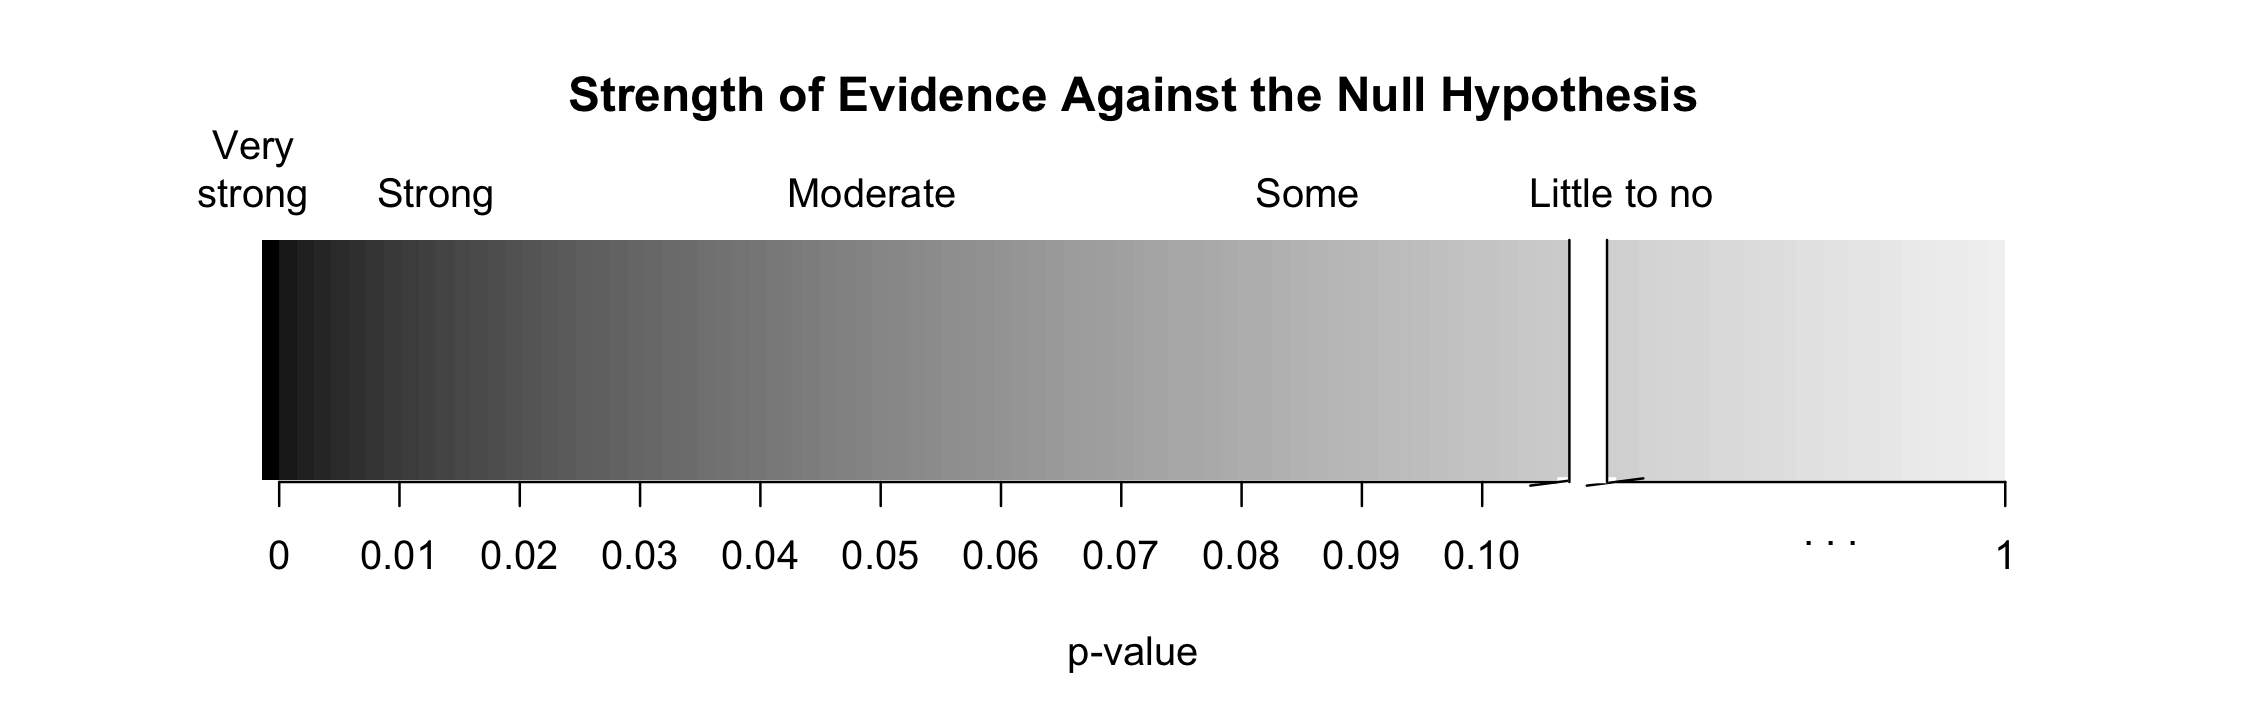
\includegraphics[width=0.75\linewidth]{images/soe_gradient_gray} \end{center}

\rgi \rgi - The \_\_\_\_\_\_\_\_\_\_\_\_\_\_\_\_\_\_the p-value, the \_\_\_\_\_\_\_\_\_\_\_\_\_\_\_\_\_\_\_ the evidence against the null hypothesis.

\begin{itemize}
\tightlist
\item
  Write a conclusion based on the p-value.
\end{itemize}

\rgi \rgi - Answers the \_\_\_\_\_\_\_\_\_\_\_\_\_\_\_\_ question.

\rgi \rgi - Amount of \_\_\_\_\_\_\_\_\_\_\_\_\_\_\_\_\_ in support of the \_\_\_\_\_\_\_\_\_\_\_\_\_\_\_\_\_ hypothesis.

\begin{itemize}
\tightlist
\item
  Decision: can we reject or fail to reject the null hypothesis?
\end{itemize}

\rgi - Significance level: cut-off of ``small'' vs ``large'' p-value

\rgi \rgi - \(\text{p-value} \le \alpha\)

\rgi \rgi \rgi - Strong enough evidence against the null hypothesis

\rgi \rgi \rgi - Decision:

\vspace{0.2in}

\rgi \rgi \rgi - Results are \_\_\_\_\_\_\_\_\_\_\_\_\_\_\_\_\_\_\_\_\_\_\_ significant.

\rgi \rgi - \(\text{p-value} > \alpha\)

\rgi \rgi \rgi - Not enough evidence against the null hypothesis

\rgi \rgi \rgi - Decision:

\vspace{0.2in}

\rgi \rgi \rgi - Results are not \_\_\_\_\_\_\_\_\_\_\_\_\_\_\_\_\_\_\_\_\_ significant.

\setstretch{1}

\hypertarget{one-proportion-test}{%
\subsection*{One proportion test}\label{one-proportion-test}}
\addcontentsline{toc}{subsection}{One proportion test}

\begin{itemize}
\item
  Reminder: review summary measures and plots discussed in the Week 3 material and Chapter 4 of the textbook.
\item
  The summary measure for a single categorical variable is a \_\_\_\_\_\_\_\_\_\_\_\_\_\_.
\end{itemize}

Notation:

\begin{itemize}
\item
  Population proportion:
\item
  Sample proportion:
\end{itemize}

Parameter of Interest:

\begin{itemize}
\item
  Include:

  \begin{itemize}
  \item
    Reference of the population (true, long-run, population, all)
  \item
    Summary measure
  \item
    Context

    \begin{itemize}
    \item
      Observational units/cases
    \item
      Response variable (and explanatory variable if present)

      \begin{itemize}
      \tightlist
      \item
        If the response variable is categorical, define a `success' in context
      \end{itemize}
    \end{itemize}
  \end{itemize}
\end{itemize}

\(\pi:\)

\vspace{0.4in}

\hypertarget{hypothesis-testing-1}{%
\subsubsection*{Hypothesis testing}\label{hypothesis-testing-1}}
\addcontentsline{toc}{subsubsection}{Hypothesis testing}

Conditions:

\begin{itemize}
\tightlist
\item
  Independence:
\end{itemize}

\vspace{0.3in}

Null hypothesis assumes ``no effect'', ``no difference'', ``nothing interesting happening'', etc.

\rgi Always of form: ``parameter'' = null value

\(H_0:\)

\vspace{0.5in}

\(H_A:\)

\vspace{0.5in}

\begin{itemize}
\tightlist
\item
  Research question determines the alternative hypothesis.
\end{itemize}

Example for class discussion: A 2007 study published in the Behavioral Ecology and Sociobiology Journal was titled ``Why do blue-eyed men prefer blue-eyed women?'' (Laeng 2007) In this study, conducted in Norway, 114 volunteer heterosexual blue-eyed males rated the attractiveness of 120 pictures of females. The researchers recorded which eye-color (blue, green, or brown) was rated the highest, on average. In the sample, 51 of the volunteers rated the blue-eyed women the most attractive. Do blue-eyed heterosexual men tend to find blue-eyed women the most attractive?

Parameter of interest:

\vspace{0.4in}

Write the null and alternative hypotheses for the blue-eyed study:

In words:

\(H_0:\)

\vspace{0.45in}

\(H_A:\)

\vspace{0.45in}

In notation:

\(H_0:\)

\vspace{0.15in}

\(H_A:\)

\vspace{0.15in}

Statistic:

\vspace{0.15in}

Is the independence condition met to analyze these data using a simulation-based approach?

\vspace{0.2in}

\hypertarget{simulation-based-method-1}{%
\subsubsection*{Simulation-based method}\label{simulation-based-method-1}}
\addcontentsline{toc}{subsubsection}{Simulation-based method}

\begin{itemize}
\item
  Simulate many samples assuming \(H_0: \pi = \pi_0\)

  \begin{itemize}
  \item
    Create a spinner with that represents the null value
  \item
    Spin the spinner \(n\) times
  \item
    Calculate and plot the simulated sample proportion from each simulation
  \item
    Repeat 1000 times (simulations) to create the null distribution
  \item
    Find the proportion of simulations at least as extreme as \(\hat{p}\)
  \end{itemize}
\end{itemize}

\begin{Shaded}
\begin{Highlighting}[]
\FunctionTok{set.seed}\NormalTok{(}\DecValTok{216}\NormalTok{)}
\FunctionTok{one\_proportion\_test}\NormalTok{(}\AttributeTok{probability\_success =} \FloatTok{0.333}\NormalTok{, }\CommentTok{\# Null hypothesis value}
          \AttributeTok{sample\_size =} \DecValTok{114}\NormalTok{, }\CommentTok{\# Enter sample size}
          \AttributeTok{number\_repetitions =} \DecValTok{1000}\NormalTok{, }\CommentTok{\# Enter number of simulations}
          \AttributeTok{as\_extreme\_as =} \FloatTok{0.447}\NormalTok{, }\CommentTok{\# Observed statistic}
          \AttributeTok{direction =} \StringTok{"greater"}\NormalTok{, }\CommentTok{\# Specify direction of alternative hypothesis}
          \AttributeTok{summary\_measure =} \StringTok{"proportion"}\NormalTok{) }\CommentTok{\# Reporting proportion or number of successes?}
\end{Highlighting}
\end{Shaded}

\begin{center}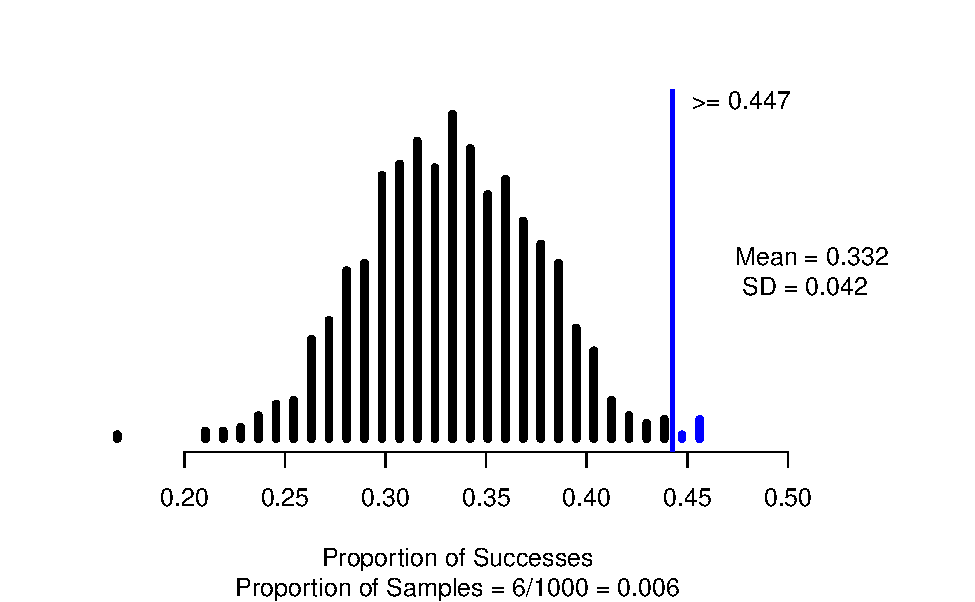
\includegraphics[width=0.7\linewidth]{06-LN06-1cat_simulation_files/figure-latex/unnamed-chunk-2-1} \end{center}

Explain why the null distribution is centered at the value of approximately 0.333:

\vspace{0.5in}

Interpretation of the p-value:

\begin{itemize}
\item
  Statement about probability or proportion of samples
\item
  Statistic (summary measure and value)
\item
  Direction of the alternative
\item
  Null hypothesis (in context)
\end{itemize}

\vspace{0.8in}

\newpage

Conclusion:

\begin{itemize}
\item
  Amount of evidence
\item
  Parameter of interest
\item
  Direction of the alternative hypothesis
\end{itemize}

\vspace{0.6in}

Generalization:

\begin{itemize}
\tightlist
\item
  Can the results of the study be generalized to the target population?
\end{itemize}

\vspace{0.4in}

\hypertarget{confidence-interval}{%
\subsection*{Confidence interval}\label{confidence-interval}}
\addcontentsline{toc}{subsection}{Confidence interval}

\rgi \(\text{statistic} \pm \text{margin of error}\)

Vocabulary:

\begin{itemize}
\tightlist
\item
  Point estimate:
\end{itemize}

\vspace{0.3in}

\begin{itemize}
\tightlist
\item
  Margin of error:
\end{itemize}

\vspace{0.3in}

\setstretch{1.5}

Purpose of a confidence interval

\begin{itemize}
\item
  To give an \_\_\_\_\_\_\_\_\_\_\_\_\_\_\_\_\_\_\_\_ \_\_\_\_\_\_\_\_\_\_\_\_\_\_\_\_\_\_\_ for the parameter of interest
\item
  Determines how \_\_\_\_\_\_\_\_\_\_\_\_\_\_ an effect is
\end{itemize}

\setstretch{1}

\hypertarget{sampling-distribution}{%
\subsubsection*{Sampling distribution}\label{sampling-distribution}}
\addcontentsline{toc}{subsubsection}{Sampling distribution}

\setstretch{1.5}

\begin{itemize}
\item
  Ideally, we would take many samples of the same \_\_\_\_\_\_\_\_\_\_\_ from the same population to create a sampling distribution
\item
  But only have 1 sample, so we will \_\_\_\_\_\_\_\_\_\_\_\_\_\_\_\_\_ with \_\_\_\_\_\_\_\_\_\_\_\_\_\_\_\_\_ from the one sample.
\item
  Need to estimate the sampling distribution to see the \_\_\_\_\_\_\_\_\_\_\_\_\_\_\_\_\_ in the sample
\end{itemize}

\setstretch{1}

\hypertarget{simulation-based-methods}{%
\subsubsection*{Simulation-based methods}\label{simulation-based-methods}}
\addcontentsline{toc}{subsubsection}{Simulation-based methods}

Bootstrap distribution:

\begin{itemize}
\item
  Write the response variable values on cards
\item
  Sample with replacement \(n\) times (bootstrapping)
\item
  Calculate and plot the simulated difference in sample means from each simulation
\item
  Repeat 1000 times (simulations) to create the bootstrap distribution
\item
  Find the cut-offs for the middle X\% (confidence level) in a bootstrap distribution.
\end{itemize}

What is bootstrapping?

\begin{itemize}
\item
  Assume the ``population'' is many, many copies of the original sample.
\item
  Randomly sample with replacement from the original sample \(n\) times.
\end{itemize}

Let's revisit the blue-eyed male study to estimate the \emph{proportion of ALL heterosexual blue-eyed males who tend to find blue-eyed women the most attractive} by creating a 90\% confidence interval.

Bootstrap distribution:

\begin{Shaded}
\begin{Highlighting}[]
\FunctionTok{set.seed}\NormalTok{(}\DecValTok{216}\NormalTok{)}
\FunctionTok{one\_proportion\_bootstrap\_CI}\NormalTok{(}\AttributeTok{sample\_size =} \DecValTok{114}\NormalTok{, }\CommentTok{\# Sample size}
                    \AttributeTok{number\_successes =} \DecValTok{51}\NormalTok{, }\CommentTok{\# Observed number of successes}
                    \AttributeTok{number\_repetitions =} \DecValTok{1000}\NormalTok{, }\CommentTok{\# Number of bootstrap samples to use}
                    \AttributeTok{confidence\_level =} \FloatTok{0.90}\NormalTok{) }\CommentTok{\# Confidence level as a decimal}
\end{Highlighting}
\end{Shaded}

\begin{center}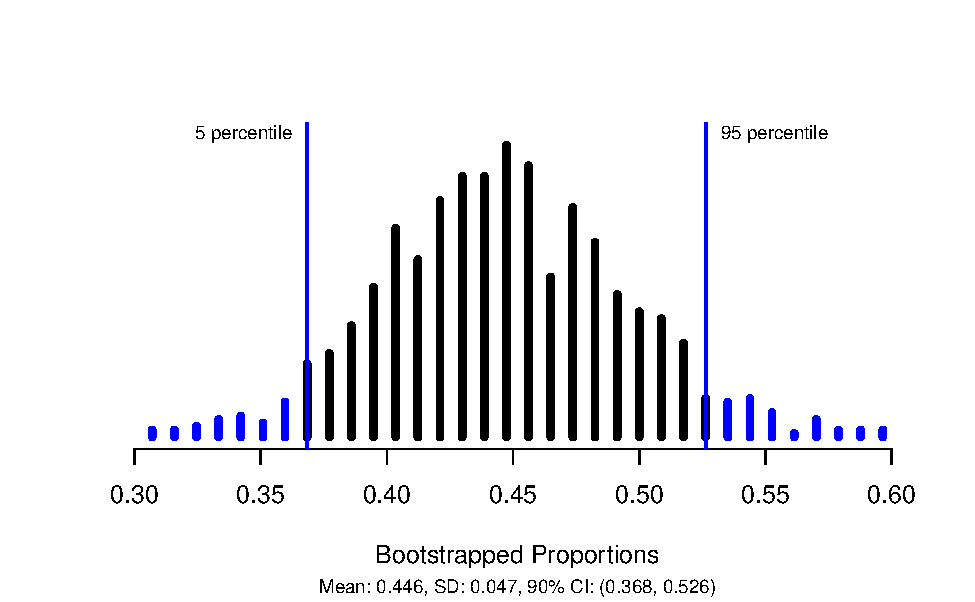
\includegraphics[width=0.7\linewidth]{06-LN06-1cat_simulation_files/figure-latex/unnamed-chunk-3-1} \end{center}

Confidence interval interpretation:

\begin{itemize}
\item
  How confident you are (e.g., 90\%, 95\%, 98\%, 99\%)
\item
  Parameter of interest
\item
  Calculated interval
\item
  Order of subtraction when comparing two groups
\end{itemize}

\vspace{0.8in}

Do the results of the confidence interval \emph{match} the results based on the p-value?

\vspace{0.5in}
\newpage

How does changing the confidence level impact the width of the confidence interval?

95\% Confidence Interval:

\begin{Shaded}
\begin{Highlighting}[]
\FunctionTok{set.seed}\NormalTok{(}\DecValTok{216}\NormalTok{)}
\FunctionTok{one\_proportion\_bootstrap\_CI}\NormalTok{(}\AttributeTok{sample\_size =} \DecValTok{114}\NormalTok{, }\CommentTok{\# Sample size}
                    \AttributeTok{number\_successes =} \DecValTok{51}\NormalTok{, }\CommentTok{\# Observed number of successes}
                    \AttributeTok{number\_repetitions =} \DecValTok{1000}\NormalTok{, }\CommentTok{\# Number of bootstrap samples to use}
                    \AttributeTok{confidence\_level =} \FloatTok{0.95}\NormalTok{) }\CommentTok{\# Confidence level as a decimal}
\end{Highlighting}
\end{Shaded}

\begin{center}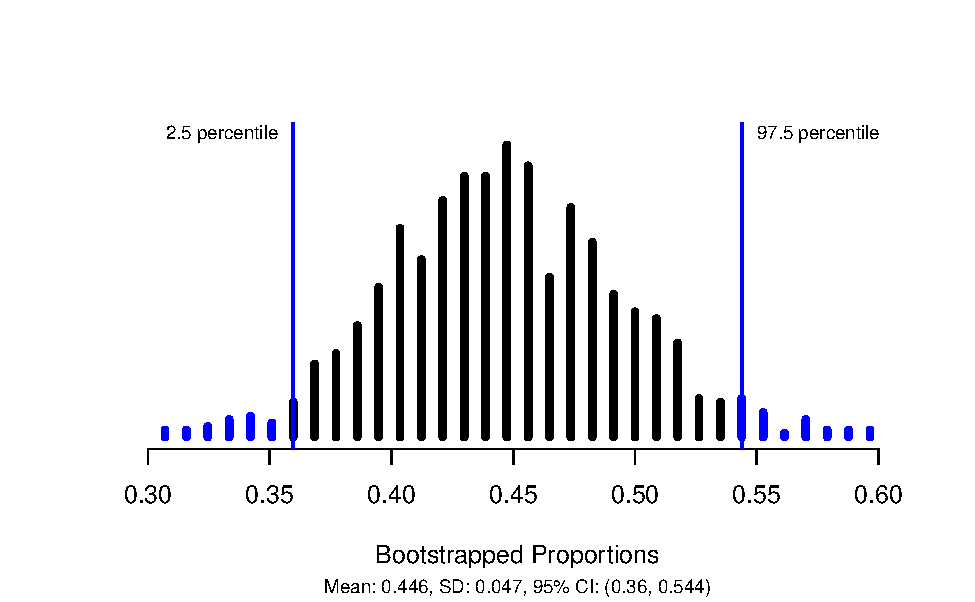
\includegraphics[width=0.7\linewidth]{06-LN06-1cat_simulation_files/figure-latex/unnamed-chunk-4-1} \end{center}

99\% Confidence Interval:

\begin{Shaded}
\begin{Highlighting}[]
\FunctionTok{set.seed}\NormalTok{(}\DecValTok{216}\NormalTok{)}
\FunctionTok{one\_proportion\_bootstrap\_CI}\NormalTok{(}\AttributeTok{sample\_size =} \DecValTok{114}\NormalTok{, }\CommentTok{\# Sample size}
                    \AttributeTok{number\_successes =} \DecValTok{51}\NormalTok{, }\CommentTok{\# Observed number of successes}
                    \AttributeTok{number\_repetitions =} \DecValTok{1000}\NormalTok{, }\CommentTok{\# Number of bootstrap samples to use}
                    \AttributeTok{confidence\_level =} \FloatTok{0.99}\NormalTok{) }\CommentTok{\# Confidence level as a decimal}
\end{Highlighting}
\end{Shaded}

\begin{center}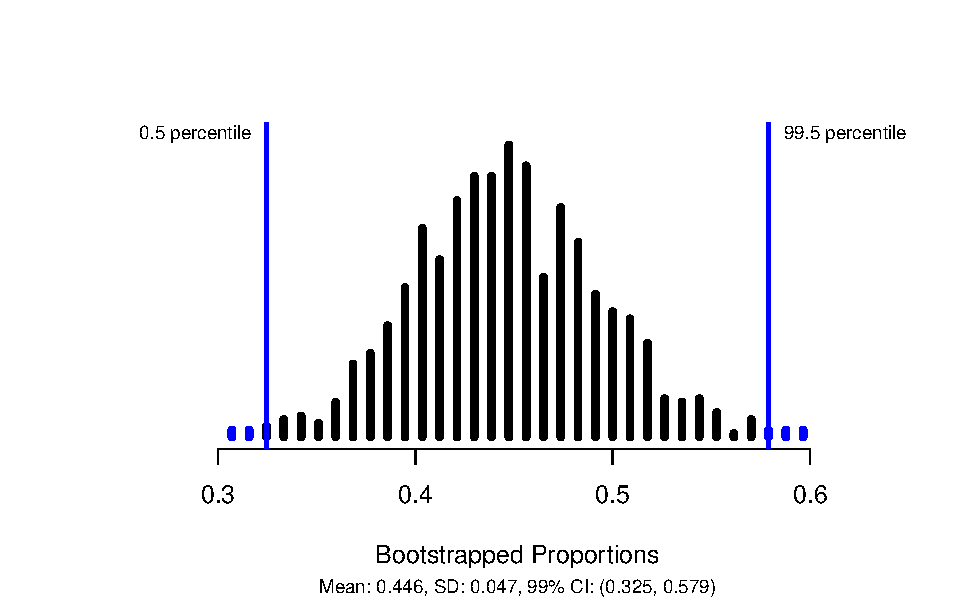
\includegraphics[width=0.7\linewidth]{06-LN06-1cat_simulation_files/figure-latex/unnamed-chunk-5-1} \end{center}

\newpage

\hypertarget{out-of-class-activity-week-6-helper-hinderer-simulation-based-confidence-interval-and-hypothesis-test}{%
\section{Out-of-Class Activity Week 6: Helper-Hinderer --- Simulation-based Confidence Interval and Hypothesis Test}\label{out-of-class-activity-week-6-helper-hinderer-simulation-based-confidence-interval-and-hypothesis-test}}

\setstretch{1}

\hypertarget{learning-outcomes-10}{%
\subsection{Learning outcomes}\label{learning-outcomes-10}}

\begin{itemize}
\item
  Use bootstrapping to find a confidence interval for a single proportion.
\item
  Interpret a confidence interval for a single proportion.
\item
  Identify the two possible explanations (one assuming the null hypothesis and one assuming the alternative hypothesis) for a relationship seen in sample data.
\item
  Given a research question involving a single categorical variable, construct the null and alternative hypotheses
  in words and using appropriate statistical symbols.
\item
  Describe and perform a simulation-based hypothesis test for a single proportion.
\end{itemize}

\hypertarget{terminology-review-9}{%
\subsection{Terminology review}\label{terminology-review-9}}

In today's activity, we will introduce simulation-based confidence intervals and hypothesis testing for a single categorical variable. Some terms covered in this activity are:

\begin{itemize}
\item
  Parameter of interest
\item
  Bootstrapping
\item
  Confidence interval
\item
  Null hypothesis
\item
  Alternative hypothesis
\item
  Simulation
\end{itemize}

To review these concepts, see Chapters 9, 10 \& 14 in your textbook.

\hypertarget{steps-of-the-statistical-investigation-process-1}{%
\subsection{Steps of the statistical investigation process}\label{steps-of-the-statistical-investigation-process-1}}

We will work through a five-step process to complete a hypothesis test for a single proportion, first introduced in the activity in week 1.

\begin{itemize}
\item
  \textbf{Ask a research question} that can be addressed by collecting data. What are the researchers trying to show?
\item
  \textbf{Design a study and collect data}. This step involves selecting the people or objects to be studied and how to gather relevant data on them.
\item
  \textbf{Summarize and visualize the data}. Calculate summary statistics and create graphical plots that best represent the research question.
\item
  \textbf{Use statistical analysis methods to draw inferences from the data}. Choose a statistical inference method appropriate for the data and identify the p-value and/or confidence interval after checking assumptions. In this study, we will focus on using randomization to generate a simulated p-value.
\item
  \textbf{Communicate the results and answer the research question}. Using the p-value and confidence interval from the analysis, determine whether the data provide statistical evidence against the null hypothesis. Write a conclusion that addresses the research question.
\end{itemize}

\newpage

\hypertarget{helper-hinderer}{%
\subsection{Helper-Hinderer}\label{helper-hinderer}}

A study by Hamblin, Wynn, and Bloom reported in Nature (Hamblin, Wynn, and Bloom 2007) was intended to check young kids' feelings about helpful and non-helpful behavior. Non-verbal infants ages 6 to 10 months were shown short videos with different shapes either helping or hindering the climber. As a class we will watch this short video to see how the experiment was run: \url{https://youtu.be/anCaGBsBOxM}. Researchers were hoping to assess: Are infants more likely to preferentially choose the helper toy over the hinderer toy? In the study, of the 16 infants age 6 to 10 months, 14 chose the \emph{helper} toy and 2 chose the \emph{hinderer} toy.

In this study, the \textbf{observational units are the infants ages 6 to 10 months}. The \textbf{variable measured on each observational unit (infant) is whether they chose the helper or the hinderer toy}. This is a categorical variable so we will be assessing the proportion of infants ages 6 to 10 months that choose the helper toy. Choosing the helper toy in this study will be considered a success.

\hypertarget{design-a-study-and-collect-data}{%
\subsubsection*{Design a study and collect data}\label{design-a-study-and-collect-data}}
\addcontentsline{toc}{subsubsection}{Design a study and collect data}

Before using statistical inference methods, we must check that the cases are independent. The sample observations are independent if the outcome of one observation does not influence the outcome of another. One way this condition is met is if data come from a simple random sample of the target population.

\begin{enumerate}
\def\labelenumi{\arabic{enumi}.}
\tightlist
\item
  Are the cases independent? Justify your answer.
\end{enumerate}

\vspace{0.8in}

\hypertarget{summarize-and-visualize-the-data}{%
\subsubsection*{Summarize and visualize the data}\label{summarize-and-visualize-the-data}}
\addcontentsline{toc}{subsubsection}{Summarize and visualize the data}

The following code reads in the data set and gives the number of infants in each level of the variable, whether the infant chose the helper or the hinderer. Remember to visually display this data we can use either a frequency bar plot or a relative frequency bar plot.

\begin{Shaded}
\begin{Highlighting}[]
 \CommentTok{\# Read in data set}
\NormalTok{infants }\OtherTok{\textless{}{-}} \FunctionTok{read.csv}\NormalTok{(}\StringTok{"https://math.montana.edu/courses/s216/data/infantchoice.csv"}\NormalTok{)}
\NormalTok{infants }\SpecialCharTok{\%\textgreater{}\%} \FunctionTok{count}\NormalTok{(choice)  }\CommentTok{\# Count number in each choice category}
\end{Highlighting}
\end{Shaded}

\begin{verbatim}
#>     choice  n
#> 1   helper 14
#> 2 hinderer  2
\end{verbatim}

\[\hat{p} = \frac{\mbox{number of successes}}{\mbox{total number of observational units}}\]
\vspace{2mm}

\begin{enumerate}
\def\labelenumi{\arabic{enumi}.}
\setcounter{enumi}{1}
\tightlist
\item
  Using the \texttt{R} output and the formula given, calculate the summary statistic (sample proportion) to represent the research question. Recall that \texttt{choosing\ the\ helper\ toy} is a considered a success. Use appropriate notation. This value is also called the \textbf{point estimate.}
\end{enumerate}

\vspace{0.5in}
\newpage

A \textbf{point estimate} (our observed statistic) provides a single plausible value for a parameter. However, a point estimate is rarely perfect; usually there is some error in the estimate. In addition to supplying a point estimate of a parameter, a next logical step would be to provide a plausible \emph{range} of values for the parameter. This plausible range of values for the population parameter is called an \textbf{interval estimate} or \textbf{confidence interval}.

For this study, the parameter of interest is the \textbf{true or population proportion of infants ages 6--10 months who will choose the helper toy}.

In today's activity, we will use bootstrapping to find a 95\% confidence interval for \(\pi\), the parameter of interest.

\begin{enumerate}
\def\labelenumi{\arabic{enumi}.}
\setcounter{enumi}{2}
\tightlist
\item
  In your own words, explain the bootstrapping process.
  \vspace{0.6in}
\end{enumerate}

\hypertarget{use-statistical-analysis-methods-to-draw-inferences-from-the-data}{%
\subsubsection*{Use statistical analysis methods to draw inferences from the data}\label{use-statistical-analysis-methods-to-draw-inferences-from-the-data}}
\addcontentsline{toc}{subsubsection}{Use statistical analysis methods to draw inferences from the data}

To use the computer simulation to create a bootstrap distribution, we will need to enter the

\begin{itemize}
\tightlist
\item
  ``sample size'' (the number of observational units or cases in the sample),
\item
  ``number of successes'' (the number of cases that choose the helper character),
\item
  ``number of repetitions'' (the number of samples to be generated), and
\item
  the ``confidence level'' (which level of confidence are we using to create the confidence interval).
\end{itemize}

\begin{enumerate}
\def\labelenumi{\arabic{enumi}.}
\setcounter{enumi}{3}
\tightlist
\item
  What values should be entered for each of the following into the simulation to create the bootstrap distribution of sample proportions to find a 95\% confidence interval?
  \vspace{1mm}
\end{enumerate}

\begin{itemize}
\tightlist
\item
  Sample size:
\end{itemize}

\vspace{.15in}

\begin{itemize}
\tightlist
\item
  Number of successes:
\end{itemize}

\vspace{.15in}

\begin{itemize}
\tightlist
\item
  Number of repetitions:
\end{itemize}

\vspace{.15in}

\begin{itemize}
\tightlist
\item
  Confidence level (as a decimal):
\end{itemize}

\vspace{.15in}

We will use the \texttt{one\_proportion\_bootstrap\_CI()} function in R (in the \texttt{catstats} package) to simulate the bootstrap distribution of sample proportions and calculate a confidence interval. Check that your answers to question 4 match what is entered in the R code.

\begin{Shaded}
\begin{Highlighting}[]
\FunctionTok{set.seed}\NormalTok{(}\DecValTok{216}\NormalTok{)}
\FunctionTok{one\_proportion\_bootstrap\_CI}\NormalTok{(}\AttributeTok{sample\_size =} \DecValTok{16}\NormalTok{, }\CommentTok{\# Sample size}
                    \AttributeTok{number\_successes =} \DecValTok{14}\NormalTok{, }\CommentTok{\# Observed number of successes}
                    \AttributeTok{number\_repetitions =} \DecValTok{1000}\NormalTok{, }\CommentTok{\# Number of bootstrap samples to use}
                    \AttributeTok{confidence\_level =} \FloatTok{0.95}\NormalTok{) }\CommentTok{\# Confidence level as a decimal}
\end{Highlighting}
\end{Shaded}

\begin{center}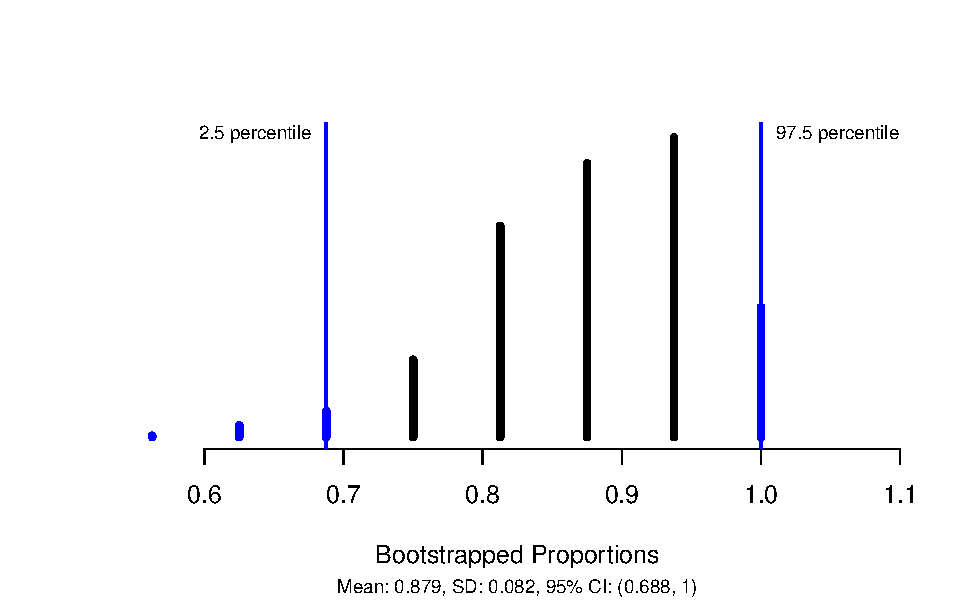
\includegraphics[width=0.7\linewidth]{06-OCA04-inference-1cat_test-simulation-S24_files/figure-latex/unnamed-chunk-2-1} \end{center}

\begin{enumerate}
\def\labelenumi{\arabic{enumi}.}
\setcounter{enumi}{4}
\item
  What is the value at the center of this bootstrap distribution? Why does this make sense?
  \vspace{.8in}
\item
  Explain why the two vertical lines are at the 2.5th percentile and the 97.5th percentile.
\end{enumerate}

\vspace{.7in}

\begin{enumerate}
\def\labelenumi{\arabic{enumi}.}
\setcounter{enumi}{6}
\tightlist
\item
  Report the 95\% bootstrapped confidence interval for \(\pi\). Use interval notation: (lower value, upper value).
\end{enumerate}

\vspace{0.2in}

\begin{enumerate}
\def\labelenumi{\arabic{enumi}.}
\setcounter{enumi}{7}
\tightlist
\item
  Interpret the 95\% confidence interval in context.
\end{enumerate}

\vspace{0.8in}

\hypertarget{use-statistical-analysis-methods-to-draw-inferences-from-the-data-1}{%
\subsubsection*{Use statistical analysis methods to draw inferences from the data}\label{use-statistical-analysis-methods-to-draw-inferences-from-the-data-1}}
\addcontentsline{toc}{subsubsection}{Use statistical analysis methods to draw inferences from the data}

In the next part of the activity, we will perform a hypothesis test to assess the research question.

\begin{enumerate}
\def\labelenumi{\arabic{enumi}.}
\setcounter{enumi}{8}
\tightlist
\item
  Identify the research question for this study. What are the researchers hoping to show?
\end{enumerate}

\vspace{0.6in}

When performing a hypothesis test, we must first identify the null hypothesis. The null hypothesis is written about the parameter of interest, or the value that summarizes the variable in the population.

If the children are just randomly choosing the toy, we would expect half (0.5) of the infants to choose the helper toy. This is the null value for our study.

\begin{enumerate}
\def\labelenumi{\arabic{enumi}.}
\setcounter{enumi}{9}
\tightlist
\item
  Using the parameter of interest given prior to question 3, write out the null hypothesis in words. That is, what do we assume to be true about the parameter of interest when we perform our simulation?
  \vspace{0.8in}
\end{enumerate}

The notation used for a population proportion (or probability, or true proportion) is \(\pi\). Since this summarizes a population, it is a parameter. When writing the \textbf{null hypothesis} in notation, we set the parameter equal to the null value, \(H_0: \pi = \pi_0\).

\begin{enumerate}
\def\labelenumi{\arabic{enumi}.}
\setcounter{enumi}{10}
\tightlist
\item
  Write the null hypothesis in notation using the null value of 0.5 in place of \(\pi_0\) in the equation given above.
\end{enumerate}

\vspace{0.2in}

The \textbf{alternative hypothesis} is the claim to be tested and the direction of the claim (less than, greater than, or not equal to) is based on the research question.

\begin{enumerate}
\def\labelenumi{\arabic{enumi}.}
\setcounter{enumi}{11}
\tightlist
\item
  Based on the research question from question 9, are we testing that the parameter is greater than 0.5, less than 0.5 or different than 0.5?
\end{enumerate}

\vspace{0.2in}

\begin{enumerate}
\def\labelenumi{\arabic{enumi}.}
\setcounter{enumi}{12}
\tightlist
\item
  Write out the alternative hypothesis in notation.
\end{enumerate}

\vspace{0.2in}

Remember that when utilizing a hypothesis test, we are evaluating two competing possibilities. For this study the \textbf{two possibilities} are either\ldots{}

\begin{itemize}
\item
  The true proportion of infants who choose the helper is 0.5 and our results just occurred by random chance; or,
\item
  The true proportion of infants who choose the helper is greater than 0.5 and our results reflect this.
\end{itemize}

Notice that these two competing possibilities represent the null and alternative hypotheses.

We will now simulate a one sample of a \textbf{null distribution} of sample proportions. The null distribution is created under the assumption the null hypothesis is true. In this case, we assume the true proportion of infants who choose the helper is 0.5, so we will create 1000 (or more) different simulations of 16 infants under this assumption.

Let's think about how to use a coin to create one simulation of 16 infants under the assumption the null hypothesis is true. Let heads equal infant chose the helper toy and tails equal infant chose the hinderer toy.

\begin{enumerate}
\def\labelenumi{\arabic{enumi}.}
\setcounter{enumi}{13}
\tightlist
\item
  How many times would you flip a coin to simulate the sample of infants?
\end{enumerate}

\vspace{0.3in}

\begin{enumerate}
\def\labelenumi{\arabic{enumi}.}
\setcounter{enumi}{14}
\tightlist
\item
  Flip a coin 16 times recording the number of times the coin lands on heads. This represents one simulated sample of 16 infants randomly choosing the toy. Calculate the proportion of coin flips that resulted in a head.
\end{enumerate}

\vspace{0.3in}

\begin{enumerate}
\def\labelenumi{\arabic{enumi}.}
\setcounter{enumi}{15}
\tightlist
\item
  Is the value from question 15 closer to 0.5, the null value, or closer to the sample proportion, 0.875?
\end{enumerate}

\vspace{0.3in}

\newpage

The distribution of the proportion of 16 coin flips from a Spring 2023 class is provided below.

\begin{center}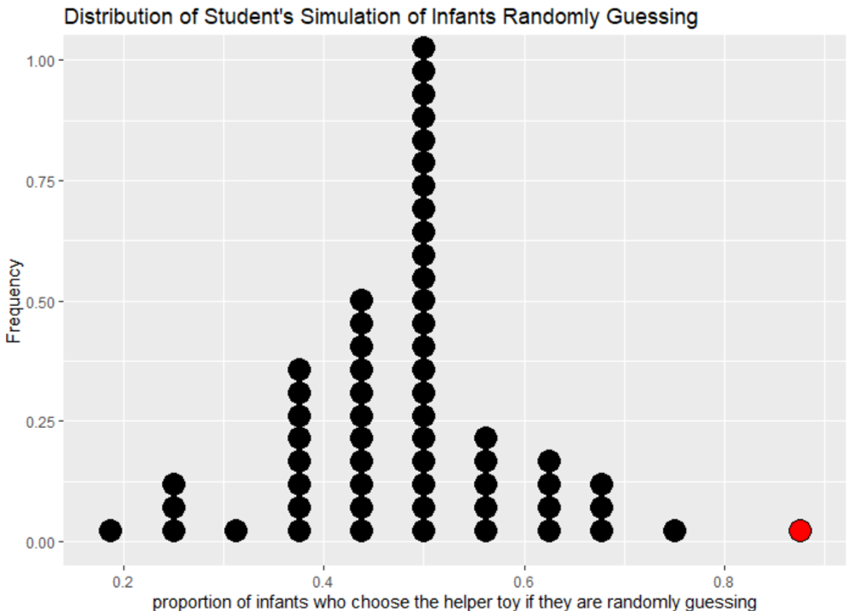
\includegraphics[width=0.75\linewidth]{images/class_simulations_oca06} \end{center}

\begin{enumerate}
\def\labelenumi{\arabic{enumi}.}
\setcounter{enumi}{16}
\tightlist
\item
  Circle the observed statistic (value from question 2) on the distribution shown above. Where does this statistic fall in this distribution: Is it near the center of the distribution (near 0.5) or in one of the tails of the distribution?
\end{enumerate}

\vspace{0.2in}

\begin{enumerate}
\def\labelenumi{\arabic{enumi}.}
\setcounter{enumi}{17}
\tightlist
\item
  Is the observed statistic (0.875) likely to happen or unlikely to happen if the true proportion of infants age 6 to 10 months who choose the helper is 0.5? Explain your answer using the plot.
\end{enumerate}

\vspace{0.8in}

In the next class, we will continue to assess the strength of evidence against the null hypothesis by using a computer to simulate 1000 samples when we assume the null hypothesis is true.

\hypertarget{take-home-messages-8}{%
\subsection{Take-home messages}\label{take-home-messages-8}}

\begin{enumerate}
\def\labelenumi{\arabic{enumi}.}
\item
  In a hypothesis test we have two competing hypotheses, the null hypothesis and the alternative hypothesis. The null hypothesis represents either a skeptical perspective or a perspective of no difference or no effect. The alternative hypothesis represents a new perspective such as the possibility that there has been a change or that there is a treatment effect in an experiment.
\item
  In a simulation-based test, we create a distribution of possible simulated statistics for our sample if the null hypothesis is true. Then we see if the calculated observed statistic from the data is likely or unlikely to occur when compared to the null distribution.
\item
  To create one simulated sample on the null distribution for a sample proportion, spin a spinner with probability equal to \(\pi_0\) (the null value), \(n\) times or draw with replacement \(n\) times from a deck of cards created to reflect \(\pi_0\) as the probability of success. Calculate and plot the proportion of successes from the simulated sample.
\item
  The goal in a hypothesis test is to assess the strength of evidence for an effect, while the goal in creating a confidence interval is to determine how large the effect is. A \textbf{confidence interval} is a range of \emph{plausible} values for the parameter of interest.
\item
  A confidence interval is built around the point estimate or observed calculated statistic from the sample. This means that the sample statistic is always the center of the confidence interval. A confidence interval includes a measure of sample to sample variability represented by the \textbf{margin of error}.
\item
  In simulation-based methods (bootstrapping), a simulated distribution of possible sample statistics is created showing the possible sample-to-sample variability. Then we find the middle \(X\) percent of the distribution around the sample statistic using the percentile method to give the range of values for the confidence interval. This shows us that we are \(X\)\% confident that the parameter is within this range, where \(X\) represents the level of confidence.
\item
  When the null value is within the confidence interval, it is a plausible value for the parameter of interest; thus, we would find a larger p-value for a hypothesis test of that null value. Conversely, if the null value is NOT within the confidence interval, we would find a small p-value for the hypothesis test and strong evidence against this null hypothesis.
\item
  To create one simulated sample on the bootstrap distribution for a sample proportion, label \(n\) cards with the original responses. Draw with replacement \(n\) times. Calculate and plot the resampled proportion of successes.
\end{enumerate}

\hypertarget{additional-notes-8}{%
\subsection{Additional notes}\label{additional-notes-8}}

Use this space to summarize your thoughts and take additional notes on today's activity and material covered.

\newpage

\hypertarget{activity-6-helper-hinderer-continued}{%
\section{Activity 6: Helper-Hinderer (continued)}\label{activity-6-helper-hinderer-continued}}

\setstretch{1}

\hypertarget{learning-outcomes-11}{%
\subsection{Learning outcomes}\label{learning-outcomes-11}}

\begin{itemize}
\item
  Describe and perform a simulation-based hypothesis test for a single proportion.
\item
  Interpret and evaluate a p-value for a simulation-based hypothesis test for a single proportion.
\item
  Explore what a p-value represents
\end{itemize}

\hypertarget{steps-of-the-statistical-investigation-process-2}{%
\subsection{Steps of the statistical investigation process}\label{steps-of-the-statistical-investigation-process-2}}

In today's activity we will continue with steps 4 and 5 in the statistical investigation process. We will continue to assess the Helper-Hinderer study from last class.

\begin{itemize}
\item
  \textbf{Ask a research question} that can be addressed by collecting data. What are the researchers trying to show?
\item
  \textbf{Design a study and collect data}. This step involves selecting the people or objects to be studied and how to gather relevant data on them.
\item
  \textbf{Summarize and visualize the data}. Calculate summary statistics and create graphical plots that best represent the research question.
\item
  \textbf{Use statistical analysis methods to draw inferences from the data}. Choose a statistical inference method appropriate for the data and identify the p-value and/or confidence interval after checking assumptions. In this study, we will focus on using randomization to generate a simulated p-value.
\item
  \textbf{Communicate the results and answer the research question}. Using the p-value and confidence interval from the analysis, determine whether the data provide statistical evidence against the null hypothesis. Write a conclusion that addresses the research question.
\end{itemize}

\hypertarget{helper-hinderer-1}{%
\subsection{Helper-Hinderer}\label{helper-hinderer-1}}

A study by Hamblin, Wynn, and Bloom reported in Nature (Hamblin, Wynn, and Bloom 2007) was intended to check young kids' feelings about helpful and non-helpful behavior. Non-verbal infants ages 6 to 10 months were shown short videos with different shapes either helping or hindering the climber. As a class we will watch this short video to see how the experiment was run: \url{https://youtu.be/anCaGBsBOxM}. Researchers were hoping to assess: Are infants more likely to preferentially choose the helper toy over the hinderer toy? In the study, of the 16 infants age 6 to 10 months, 14 chose the \emph{helper} toy and 2 chose the \emph{hinderer} toy.

\begin{enumerate}
\def\labelenumi{\arabic{enumi}.}
\tightlist
\item
  Report the sample proportion calculated in the out of class activity.
\end{enumerate}

\vspace{0.3in}

\begin{enumerate}
\def\labelenumi{\arabic{enumi}.}
\setcounter{enumi}{1}
\tightlist
\item
  Write the alternative hypothesis in words in context of the problem. Remember the direction we are testing is dependent on the research question.
\end{enumerate}

\vspace{0.8in}

Today, we will use the computer to simulate a null distribution of 1000 different samples of 16 infants, plotting the proportion who chose the helper in each sample, based on the assumption that the true proportion of infants who choose the helper is 0.5 (or that the null hypothesis is true).

\newpage

To use the computer simulation, we will need to enter the

\begin{itemize}
\tightlist
\item
  assumed ``probability of success'' (\(\pi_0\)),
\item
  ``sample size'' (the number of observational units or cases in the sample),
\item
  ``number of repetitions'' (the number of samples to be generated),
\item
  ``as extreme as'' (the observed statistic), and
\item
  the ``direction'' (matches the direction of the alternative hypothesis).
\end{itemize}

\begin{enumerate}
\def\labelenumi{\arabic{enumi}.}
\setcounter{enumi}{2}
\tightlist
\item
  What values should be entered for each of the following into the one proportion test to create 1000 simulations?
\end{enumerate}

\vspace{1mm}

\begin{itemize}
\tightlist
\item
  Probability of success:
\end{itemize}

\vspace{.2in}

\begin{itemize}
\tightlist
\item
  Sample size:
\end{itemize}

\vspace{.2in}

\begin{itemize}
\tightlist
\item
  Number of repetitions:
\end{itemize}

\vspace{.2in}

\begin{itemize}
\tightlist
\item
  As extreme as:
\end{itemize}

\vspace{.2in}

\begin{itemize}
\tightlist
\item
  Direction (\texttt{"greater"}, \texttt{"less"}, or \texttt{"two-sided"}):
\end{itemize}

We will use the \texttt{one\_proportion\_test()} function in \texttt{R} (in the \texttt{catstats} package) to simulate the null distribution of sample proportions and compute a p-value. Using the provided \texttt{R} script file, fill in the values/words for each \texttt{xx} with your answers from question 3 in the one proportion test to create a null distribution with 1000 simulations. Then highlight and run lines 1--16.

\begin{Shaded}
\begin{Highlighting}[]
\FunctionTok{one\_proportion\_test}\NormalTok{(}\AttributeTok{probability\_success =}\NormalTok{ xx, }\CommentTok{\# Null hypothesis value}
          \AttributeTok{sample\_size =}\NormalTok{ xx, }\CommentTok{\# Enter sample size}
          \AttributeTok{number\_repetitions =} \DecValTok{1000}\NormalTok{, }\CommentTok{\# Enter number of simulations}
          \AttributeTok{as\_extreme\_as =}\NormalTok{ xx, }\CommentTok{\# Observed statistic}
          \AttributeTok{direction =} \StringTok{"xx"}\NormalTok{, }\CommentTok{\# Specify direction of alternative hypothesis}
          \AttributeTok{summary\_measure =} \StringTok{"proportion"}\NormalTok{) }\CommentTok{\# Reporting proportion or number of successes?}
\end{Highlighting}
\end{Shaded}

\begin{enumerate}
\def\labelenumi{\arabic{enumi}.}
\setcounter{enumi}{3}
\tightlist
\item
  Sketch the null distribution created from the \texttt{R} code here.
\end{enumerate}

\vspace{1.8in}

\begin{enumerate}
\def\labelenumi{\arabic{enumi}.}
\setcounter{enumi}{4}
\tightlist
\item
  Around what value is the null distribution centered? Why does that make sense?
\end{enumerate}

\vspace{1in}

\begin{enumerate}
\def\labelenumi{\arabic{enumi}.}
\setcounter{enumi}{5}
\tightlist
\item
  Circle the observed statistic (value from question 1) on the distribution you drew in question 4. Where does this statistic fall in the null distribution: Is it near the center of the distribution (near 0.5) or in one of the tails of the distribution?
\end{enumerate}

\vspace{0.2in}

\begin{enumerate}
\def\labelenumi{\arabic{enumi}.}
\setcounter{enumi}{6}
\tightlist
\item
  Is the observed statistic likely to happen or unlikely to happen if the true proportion of infants who choose the helper is 0.5? Explain your answer using the plot.
\end{enumerate}

\vspace{0.5in}

\begin{enumerate}
\def\labelenumi{\arabic{enumi}.}
\setcounter{enumi}{7}
\tightlist
\item
  Using the simulation, what is the proportion of simulated samples that generated a sample proportion at the observed statistic or greater, if the true proportion of infants who choose the helper is 0.5? \emph{Hint}: Look under the simulation.
\end{enumerate}

\vspace{0.2in}

The value in question 8 is the \textbf{p-value}. The smaller the p-value, the more evidence we have against the null hypothesis.

\begin{enumerate}
\def\labelenumi{\arabic{enumi}.}
\setcounter{enumi}{8}
\tightlist
\item
  Using the following guidelines for the strength of evidence, how much evidence do the data provide against the null hypothesis? (Circle one of the five descriptions.)
\end{enumerate}

\begin{center}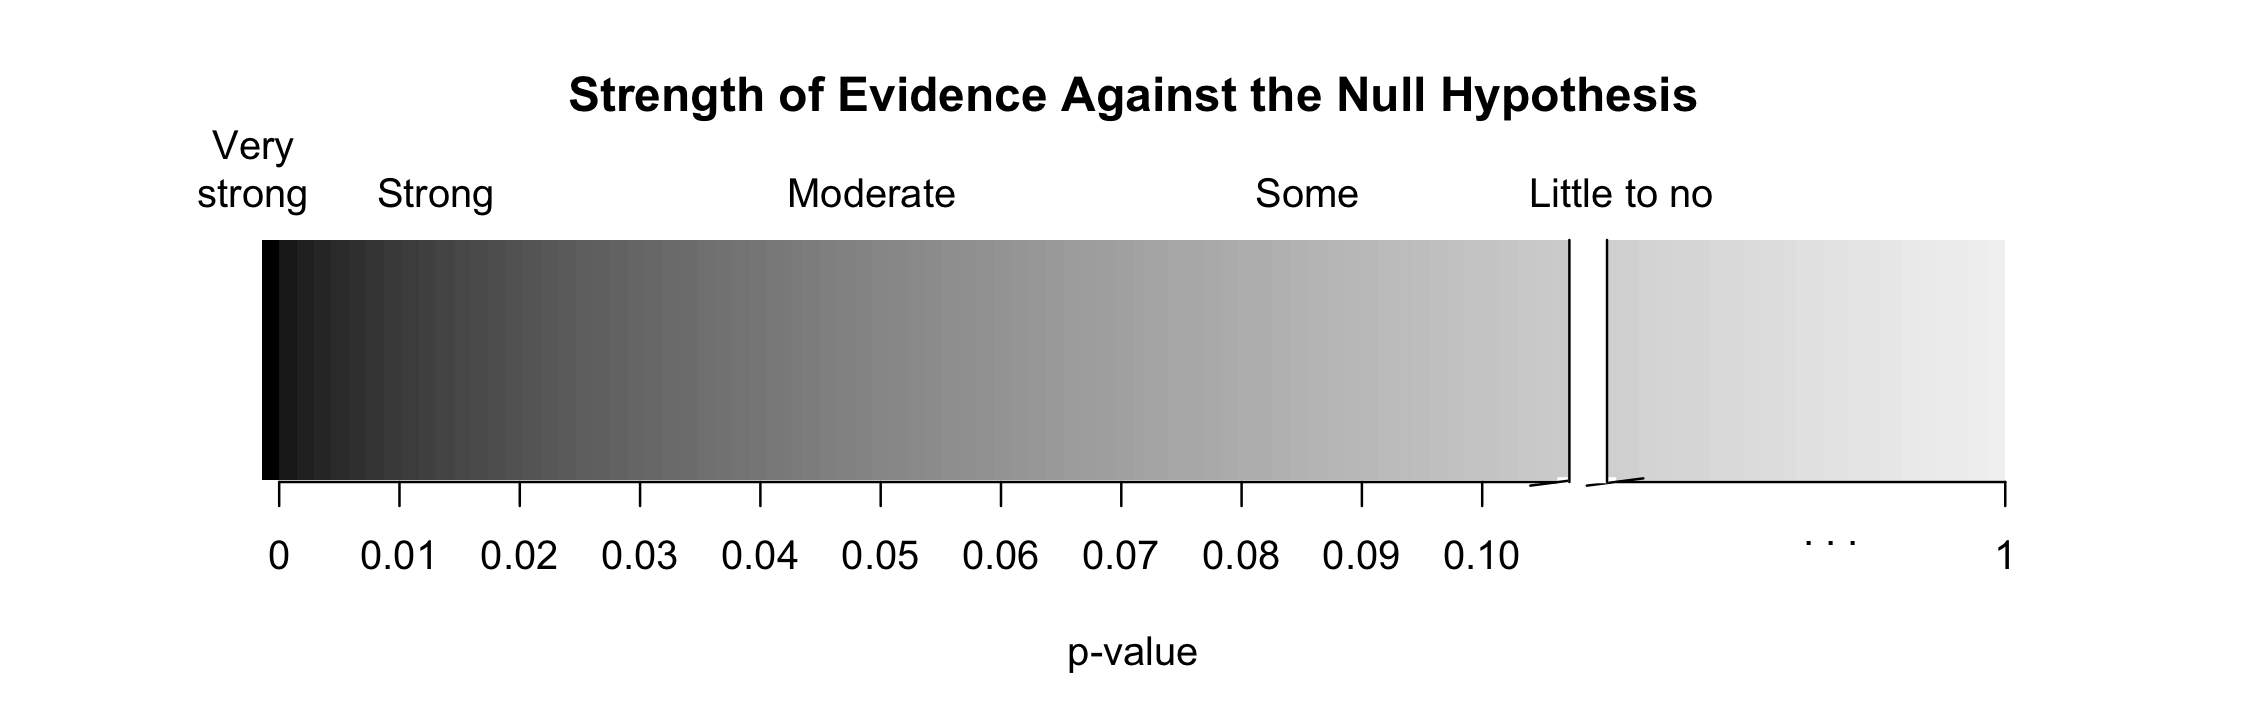
\includegraphics[width=0.9\linewidth]{images/soe_gradient_gray} \end{center}

\hypertarget{interpret-the-p-value}{%
\subsubsection*{Interpret the p-value}\label{interpret-the-p-value}}
\addcontentsline{toc}{subsubsection}{Interpret the p-value}

The p-value measures the probability that we observe a sample proportion as extreme as what was seen in the data or more extreme (matching the direction of the Ha) IF the null hypothesis is true.

\begin{enumerate}
\def\labelenumi{\arabic{enumi}.}
\setcounter{enumi}{9}
\tightlist
\item
  What did we assume to create the null distribution?
\end{enumerate}

\vspace{0.7in}

\begin{enumerate}
\def\labelenumi{\arabic{enumi}.}
\setcounter{enumi}{10}
\tightlist
\item
  What value did we compare to the null distribution to find the p-value?
\end{enumerate}

\vspace{0.3in}

\begin{enumerate}
\def\labelenumi{\arabic{enumi}.}
\setcounter{enumi}{11}
\tightlist
\item
  What direction did we count simulations from the statistic?
  \vspace{0.3in}
\end{enumerate}

\newpage

\begin{enumerate}
\def\labelenumi{\arabic{enumi}.}
\setcounter{enumi}{12}
\tightlist
\item
  Fill in the blanks below to interpret the p-value.
\end{enumerate}

\setstretch{1.5}

We would observe a sample proportion of (value of the sample proportion )\hrulefill  

or (greater, less, more extreme) \hrulefill   

with a probability of (value of p-value) \hrulefill  

IF we assume (\(H_0\) in context) \hrulefill.

\setstretch{1}
\vspace{12pt}

\hypertarget{communicate-the-results-and-answer-the-research-question}{%
\subsubsection*{Communicate the results and answer the research question}\label{communicate-the-results-and-answer-the-research-question}}
\addcontentsline{toc}{subsubsection}{Communicate the results and answer the research question}

When we write a conclusion we answer the research question by stating how much evidence there is for the alternative hypothesis.

\begin{enumerate}
\def\labelenumi{\arabic{enumi}.}
\setcounter{enumi}{13}
\tightlist
\item
  Write a conclusion in context of the study. How much evidence does the data provide in support of the alternative hypothesis?
\end{enumerate}

\vspace{0.6in}

\setstretch{1.5}

\begin{enumerate}
\def\labelenumi{\arabic{enumi}.}
\setcounter{enumi}{14}
\tightlist
\item
  Fill in the blanks below to write a paragraph summarizing the results of the study as if writing a press release.
\end{enumerate}

Researchers were interested if infants observe social cues and would be more likely to choose the helper toy over the hinderer toy. In a sample of (sample size) \_\_\_\_\_\_\_\_\_\_\_\_\_infants, (number of successes) \_\_\_\_\_\_\_\_\_\_\_\_\_\_\_chose the helper toy. A simulation null distribution with 1000 simulations was created in RStudio. The p-value was found by calculating the proportion of simulations in the null distribution at the sample statistic of 0.875 and greater. This resulted in a p-value of (value of p-value)\_\_\_\_\_\_\_\_\_\_\_\_\_\_\_. We would observe a sample proportion of (value of the sample proportion) \_\_\_\_\_\_\_\_\_\_\_\_\_\_\_\_\_\_\_\_\_\_ or (greater, less, more extreme) \_\_\_\_\_\_\_\_\_\_\_\_\_\_\_\_\_\_\_\_\_ with a probability of (value of p-value)\_\_\_\_\_\_\_\_\_\_\_\_\_\_\_\_\_\_\_\\
IF we assume (\(H_0\) in context) \_\_\_\_\_\_\_\_\_\_\_\_\_\_\_\_\_\_\_\_\_\_\_\_\_\_\_\_\_\_\_\_\_\_\_\_\_\_\_\_\_\_\_\_.
Based on this p-value, there is (very strong/little to no) \_\_\_\_\_\_\_\_\_\_\_\_\_\_\_\_\_\_\_\_\_\_ evidence that the (sample/true)\_\_\_\_\_\_\_\_\_\_\_\_\_\_\_\_\_\_\_\_\_ proportion of infants age 6 to 10 months who will choose the helper toy is (greater than, less than, not equal to) \_\_\_\_\_\_\_\_\_\_\_\_\_\_\_\_\_\_\_\_\_ 0.5. In addition, a 95\% confidence interval was found for the parameter of interest. We are 95\% confident that the (true/sample)\_\_\_\_\_\_\_\_\_\_\_\_\_\_\_\_\_\_\_\_\_\_\_\_\_ proportion of infants age 6 to 10 months who will choose the helper toy is between (lower value)\_\_\_\_\_\_\_\_\_\_\_\_\_\_\_\_ and (upper value)\_\_\_\_\_\_\_\_\_\_\_\_\_\_\_\_\_\_\_\_. The results of this study can be generalized to (all infants age 6 to 10 months/infants similar to those in this study)\_\_\_\_\_\_\_\_\_\_\_\_\_\_\_\_\_\_\_\_\_\_\_\_\_\_\_ as the researchers (did/did not)\_\_\_\_\_\_\_\_\_\_\_\_\_\_\_\_\_\_\_\_\_ select a random sample.

\setstretch{1}

\hypertarget{take-home-messages-9}{%
\subsection{Take-home messages}\label{take-home-messages-9}}

\begin{enumerate}
\def\labelenumi{\arabic{enumi}.}
\item
  The null distribution is created based on the assumption the null hypothesis is true. We compare the sample statistic to the distribution to find the likelihood of observing this statistic.
\item
  The p-value measures the probability of observing the sample statistic or more extreme (in direction of the alternative hypothesis) is the null hypothesis is true.
\end{enumerate}

\hypertarget{additional-notes-9}{%
\subsection{Additional notes}\label{additional-notes-9}}

Use this space to summarize your thoughts and take additional notes on today's activity and material covered.

\newpage

\hypertarget{inference-for-a-single-categorical-variable-theory-based-methods-errors-and-power}{%
\chapter{Inference for a Single Categorical Variable: Theory-based Methods + Errors and Power}\label{inference-for-a-single-categorical-variable-theory-based-methods-errors-and-power}}

\hypertarget{lecture-notes-week-7-inference-for-one-categorical-variable-using-theory-based-methods}{%
\section{Lecture Notes Week 7: Inference for One Categorical Variable using Theory-based Methods}\label{lecture-notes-week-7-inference-for-one-categorical-variable-using-theory-based-methods}}

\setstretch{1}

\hypertarget{theory-based-methods}{%
\subsection*{Theory-based methods}\label{theory-based-methods}}
\addcontentsline{toc}{subsection}{Theory-based methods}

\hypertarget{central-limit-theorem}{%
\subsubsection*{Central limit theorem}\label{central-limit-theorem}}
\addcontentsline{toc}{subsubsection}{Central limit theorem}

The Central Limit Theorem tells us that the \_\_\_\_\_\_\_\_\_\_\_\_\_\_ distribution of a sample proportion (and sample mean and sample differences) will be approximately \_\_\_\_\_\_\_\_\_\_\_\_\_\_ if the sample size is \_\_\_\_\_\_\_\_\_\_\_\_\_\_ \_\_\_\_\_\_\_\_\_\_\_\_\_\_\_\_.

The \_\_\_\_\_\_\_\_\_\_\_\_\_\_ of distribution of sample proportions (sampling distribution) from thousands of samples will be bell-shaped/symmetric (Normal), if the sample size is large enough and the observations are \_\_\_\_\_\_\_\_\_\_\_\_\_\_\_\_.

\begin{itemize}
\tightlist
\item
  \(\hat{p} \sim N (\pi, \sqrt{\frac{\pi \times (1-\pi)}{n}})\)
\end{itemize}

Conditions of the CLT:

\begin{itemize}
\tightlist
\item
  Independence (\emph{also must be met to use simulation methods}): the response for one observational unit will not influence another observational unit
\end{itemize}

\vspace{1mm}

\begin{itemize}
\tightlist
\item
  Large enough sample size:
\end{itemize}

\vspace{0.3in}

Normal distribution:

\begin{itemize}
\item
  Bell-shaped and \_\_\_\_\_\_\_\_\_\_\_\_\_\_
\item
  Standard normal distribution: \(N(0,1)\)
\end{itemize}

\begin{figure}

{\centering 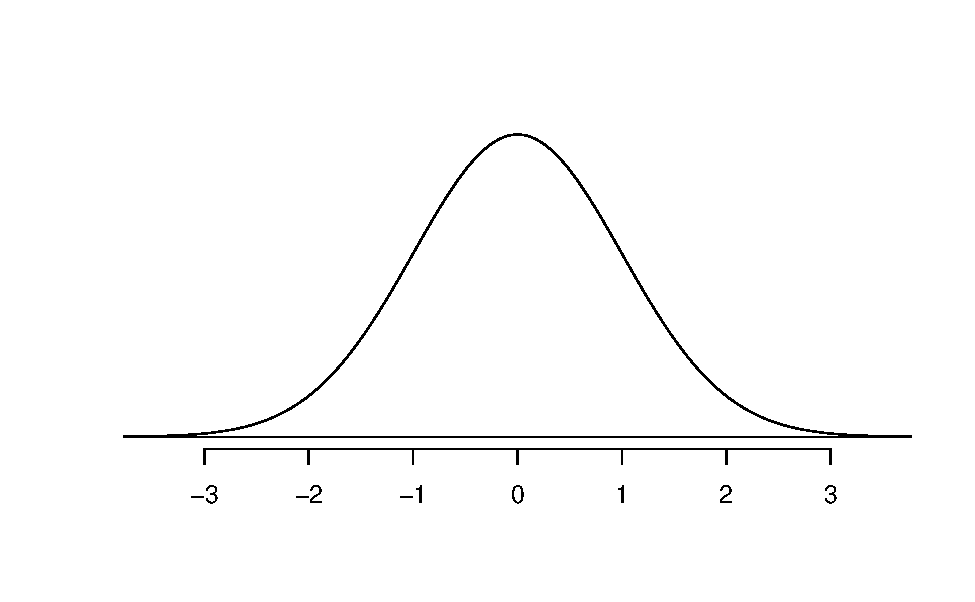
\includegraphics[width=0.5\linewidth]{07-LN07-1cat_theory_files/figure-latex/simpleNormalc-1} 

}

\caption{A standard normal curve.}\label{fig:simpleNormalc}
\end{figure}

Standardized statistic: Z - score

\vspace{1mm}

\begin{itemize}
\tightlist
\item
  \(Z = \frac{\mbox{statistic} - \mbox{null value}}{\mbox{standard error of the statistic}}\)
\end{itemize}

\vspace{0.5in}

\begin{itemize}
\tightlist
\item
  Measures the \_\_\_\_\_\_\_\_\_\_\_ of standard \_\_\_\_\_\_\_\_\_\_\_\_\_ the statistic is from the null value
\end{itemize}

\hypertarget{rule}{%
\subsection*{68-95-99.7 Rule}\label{rule}}
\addcontentsline{toc}{subsection}{68-95-99.7 Rule}

\begin{itemize}
\item
  68\% of Normal distribution within 1 SD of the mean (mean -- SD, mean + SD)
\item
  95\% within (mean -- 2SD, mean + 2SD)
\item
  99.7\% within (mean -- 3SD, mean + 3SD)
\end{itemize}

\begin{center}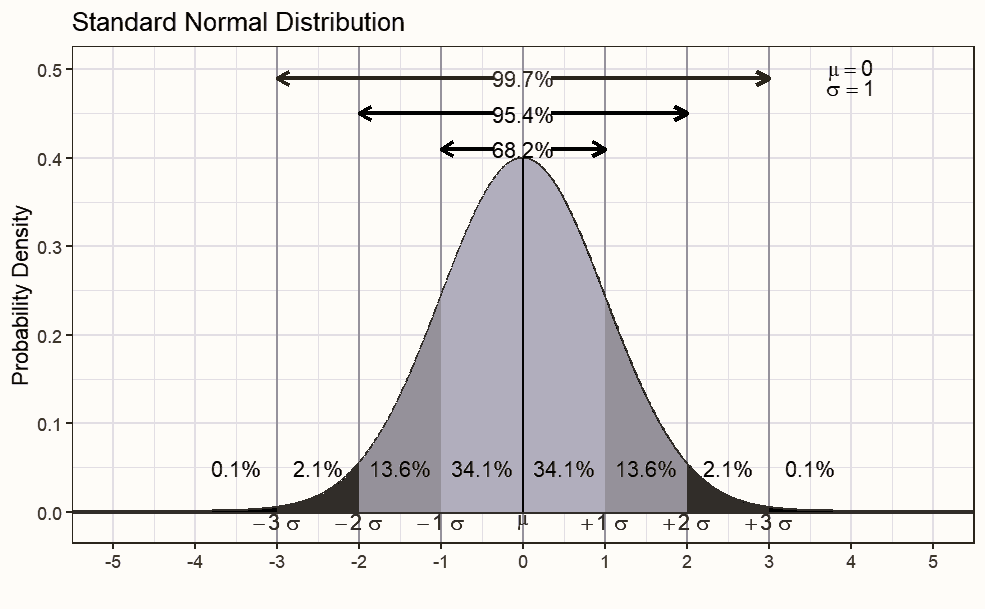
\includegraphics[width=0.65\linewidth]{images/Empirical_Rule_Mark_bw} \end{center}

General steps of a hypothesis test

\begin{enumerate}
\def\labelenumi{\arabic{enumi}.}
\item
  Write a research question and hypotheses.
\item
  Collect data and calculate a summary statistic.
\item
  Model a sampling distribution which assumes the null hypothesis is true.
\item
  Calculate a p-value.
\item
  Draw conclusions based on a p-value.
\end{enumerate}

\hypertarget{theory-based-methods-for-a-single-categorical-variable}{%
\subsubsection*{Theory-based methods for a single categorical variable}\label{theory-based-methods-for-a-single-categorical-variable}}
\addcontentsline{toc}{subsubsection}{Theory-based methods for a single categorical variable}

Conditions for inference using theory-based methods:

\begin{itemize}
\item
  Independence:

  \begin{itemize}
  \tightlist
  \item
    The outcome of one observation does not influence the outcome of another.
  \item
    Taking a random sample is one way to satisfy this condition.
  \end{itemize}
\item
  Large enough sample size:
\end{itemize}

\vspace{1in}

\begin{itemize}
\item
  Calculate the standardized statistic
\item
  Find the area under the standard normal distribution at least as extreme as the standardized statistic
\end{itemize}

Equation for the standard error of the sample proportion assuming the null hypothesis is true:

\vspace{0.5in}

\setstretch{1.5}

\begin{itemize}
\tightlist
\item
  This value measures how far each possible sample \_\_\_\_\_\_\_\_\_\_\_\_\_ is from the \_\_\_\_\_\_\_\_\_ value, on average.
\end{itemize}

\setstretch{1}

Equation for the standardized sample proportion:

\vspace{0.5in}

\setstretch{1.5}

\begin{itemize}
\tightlist
\item
  This value measures how many \_\_\_\_\_\_\_\_\_\_\_\_\_ deviations the sample \_\_\_\_\_\_\_\_\_\_\_\_\_ is above/below the \_\_\_\_\_\_\_\_\_\_ value.
\end{itemize}

\setstretch{1}

Example for Class Discussion: The American Red Cross reports that 10\% of US residents eligible to donate blood actually do donate. A poll conducted on a representative of 200 Montana residents eligible to donate blood found that 33 had donated blood sometime in their life. Do Montana residents donate at a different rate than US population?

Are the conditions met to analyze the blood donations data using theory-based methods?

\vspace{1in}

Hypotheses:

In notation:

\(H_0:\)

\vspace{0.2in}

\(H_A:\)

\vspace{0.2in}

In words:

\(H_0:\)

\vspace{0.6in}

\(H_A:\)

\vspace{0.6in}

\newpage

Calculate the standardized sample proportion of Montana residents that have donated blood sometime in their life.

\begin{itemize}
\tightlist
\item
  First calculate the standard error of the sample proportion assuming the null hypothesis is true
\end{itemize}

\vspace{0.5in}

\begin{itemize}
\tightlist
\item
  Then calculate the Z score.
\end{itemize}

\vspace{0.5in}

\begin{center}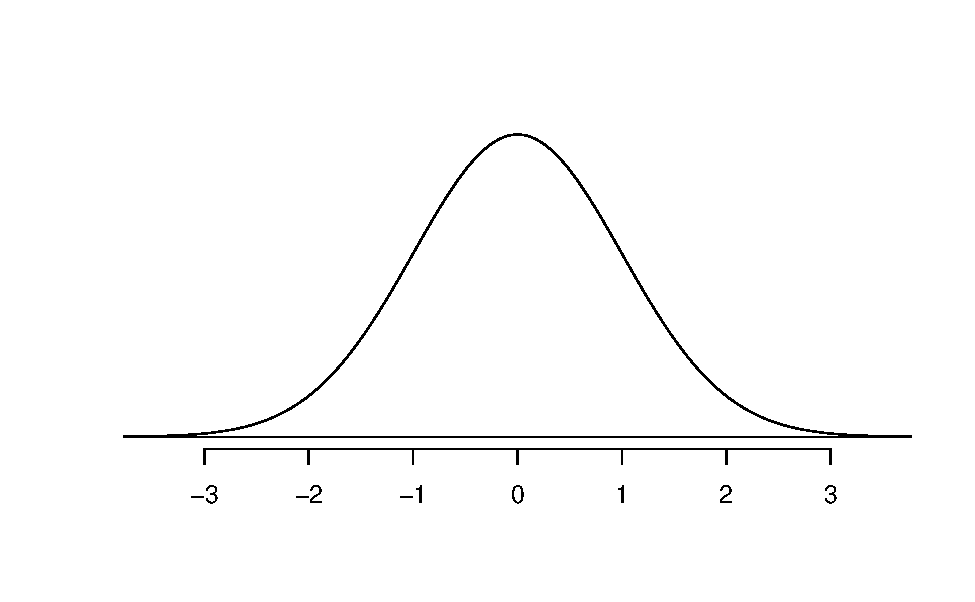
\includegraphics[width=0.5\linewidth]{07-LN07-1cat_theory_files/figure-latex/standNormalc-1} \end{center}

Interpret the standardized statistic

\vspace{0.5in}

To find the p-value, find the area under the standard normal distribution at the standardized statistic and more extreme.

\begin{Shaded}
\begin{Highlighting}[]
\FunctionTok{pnorm}\NormalTok{(}\FloatTok{3.064}\NormalTok{, }\AttributeTok{lower.tail =} \ConstantTok{FALSE}\NormalTok{)}\SpecialCharTok{*}\DecValTok{2}
\CommentTok{\#\textgreater{} [1] 0.002183989}
\end{Highlighting}
\end{Shaded}

Interpretation of the p-value:

\begin{itemize}
\item
  Statement about probability or proportion of samples
\item
  Statistic (summary measure and value)
\item
  Direction of the alternative
\item
  Null hypothesis (in context)
\end{itemize}

\vspace{0.6in}

Conclusion:

\begin{itemize}
\item
  Amount of evidence
\item
  Parameter of interest
\item
  Direction of the alternative hypothesis
\end{itemize}

\vspace{0.5in}

Decision at a significance level of 0.05 \((\alpha = 0.05)\):

\vspace{0.3in}

Generalization:

\begin{itemize}
\tightlist
\item
  Can the results of the study be generalized to the target population?
\end{itemize}

\vspace{0.4in}

\hypertarget{confidence-interval-1}{%
\subsection*{Confidence interval}\label{confidence-interval-1}}
\addcontentsline{toc}{subsection}{Confidence interval}

\begin{itemize}
\item
  Interval of \_\_\_\_\_\_\_\_\_\_ values for the parameter of interest
\item
  \(CI = \text{statistic} \pm \text{margin of error}\)
\end{itemize}

\vspace{0.5in}

\hypertarget{theory-based-method-for-a-single-categorical-variable}{%
\subsubsection*{Theory-based method for a single categorical variable}\label{theory-based-method-for-a-single-categorical-variable}}
\addcontentsline{toc}{subsubsection}{Theory-based method for a single categorical variable}

\begin{itemize}
\item
  \(CI = \hat{p} \pm (z^* \times SE(\hat{p}))\)
\item
  Multiplier (\(z^*\)) is the value at a certain \_\_\_\_\_\_\_\_\_\_\_\_ under the standard normal distribution
\end{itemize}

\begin{center}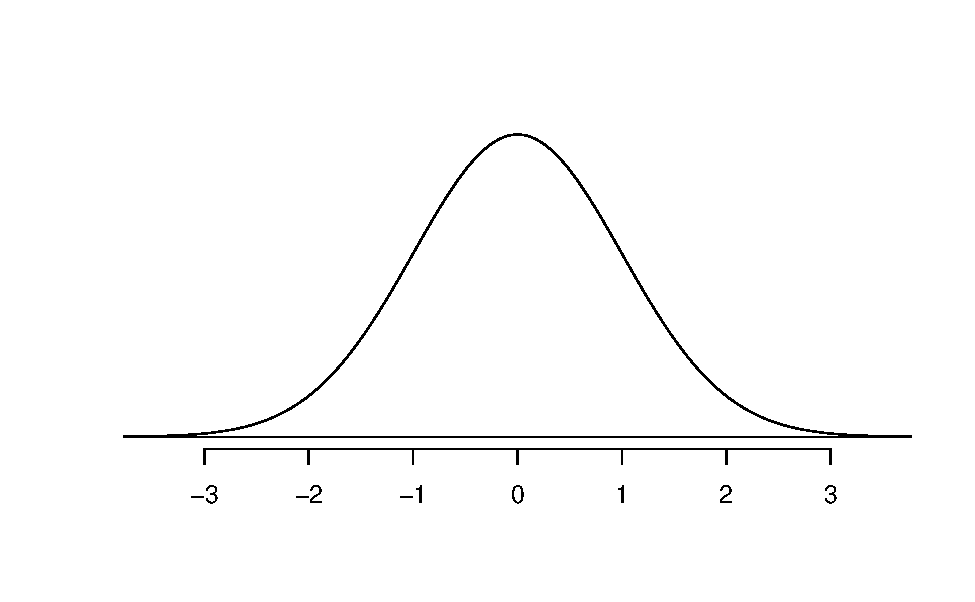
\includegraphics[width=0.5\linewidth]{07-LN07-1cat_theory_files/figure-latex/standardNormalcur-1} \end{center}

For a 95\% confidence interval:

\begin{Shaded}
\begin{Highlighting}[]
\FunctionTok{qnorm}\NormalTok{(}\FloatTok{0.975}\NormalTok{, }\AttributeTok{lower.tail=}\ConstantTok{TRUE}\NormalTok{)}
\CommentTok{\#\textgreater{} [1] 1.959964}
\end{Highlighting}
\end{Shaded}

\setstretch{1.5}

\begin{itemize}
\tightlist
\item
  When creating a confidence interval, we no longer assume the \_\_\_\_\_\_\_\_\_\_\_\_\_ hypothesis is true. Use \_\_\_\_\_\_\_\_ to calculate the sample to sample variability, rather than \(\pi_0\).
\end{itemize}

\setstretch{1}

Equation for the standard error of the sample proportion \emph{NOT} assuming the null is true:

\vspace{0.5in}

\newpage

Example: Estimate the true proportion of Montana residents that have donated blood at least once in their life.

Find a 95\% confidence interval:

\vspace{1in}

Confidence interval interpretation:

\begin{itemize}
\item
  How confident you are (e.g., 90\%, 95\%, 98\%, 99\%)
\item
  Parameter of interest
\item
  Calculated interval
\item
  Order of subtraction when comparing two groups
\end{itemize}

\vspace{0.8in}

\hypertarget{interpreting-confidence-level}{%
\subsubsection*{Interpreting confidence level}\label{interpreting-confidence-level}}
\addcontentsline{toc}{subsubsection}{Interpreting confidence level}

\setstretch{1.5}

What does it mean to be 95\% confident in a created confidence interval?

\begin{itemize}
\item
  Our goal is to only take \_\_\_\_\_\_\_\_ sample from the \_\_\_\_\_\_\_\_\_\_\_\_\_ to create a \_\_\_\_\_\_\_\_\_\_\_\_\_ interval.
\item
  Based on the 68-95-99.7 rule, we know that approximately \_\_\_\_\_\_\% of sample \_\_\_\_\_\_\_\_\_\_\_\_\_\_ will fall within \_\_\_\_\_\_\_\_\_\_ from the parameter.
\item
  If we create 95\% confidence intervals, \_\_\_\_\_\_\_\_\% of samples will create a 95\% \_\_\_\_\_\_\_\_\_\_\_\_\_\_ interval that will contain the \_\_\_\_\_\_\_\_\_\_\_\_\_ of interest.
\item
  95\% of samples accurately \_\_\_\_\_\_\_\_\_\_\_\_\_\_ the parameter of interest

  \begin{itemize}
  \tightlist
  \item
    When we create one confidence interval, we are 95\% \_\_\_\_\_\_\_\_\_\_\_\_\_\_\_\_ that we have a ``good'' sample that created a confidence interval that contains the \_\_\_\_\_\_\_\_\_\_\_ of interest.
  \end{itemize}
\end{itemize}

\setstretch{1}

Interpret the confidence \textbf{level} for the blood donation study.

\vspace{0.5in}

\newpage

\hypertarget{errors-power-and-practical-importance}{%
\subsection*{Errors, power, and practical importance}\label{errors-power-and-practical-importance}}
\addcontentsline{toc}{subsection}{Errors, power, and practical importance}

\setstretch{1.5}

Type 1 Error: \_\_\_\_\_\_\_\_\_\_\_ the null hypothesis, when the null is \_\_\_\_\_\_\_\_\_\_\_\_.

\begin{itemize}
\item
  Only can have a Type 1 Error when we make the \_\_\_\_\_\_\_\_\_\_\_\_ to \_\_\_\_\_\_\_\_\_\_\_\_ the null hypothesis.
\item
  The probability of a Type 1 Error is \(\alpha\), the \_\_\_\_\_\_\_\_\_\_\_\_ level
\end{itemize}

Type 2 Error: \_\_\_\_\_\_\_\_\_\_\_ to reject the null hypothesis, when the null is \_\_\_\_\_\_\_\_\_\_.

\begin{itemize}
\tightlist
\item
  Only can have a Type 2 Error when we make the \_\_\_\_\_\_\_\_\_\_\_\_ to \_\_\_\_\_\_\_\_\_\_\_\_ to reject the null hypothesis.
\end{itemize}

Power: probability of \_\_\_\_\_\_\_\_\_\_\_ the null hypothesis, when the null is \_\_\_\_\_\_\_\_\_\_\_\_\_.

\vspace{1.5in}

Increasing power:

\begin{itemize}
\item
  Increase \_\_\_\_\_\_\_\_\_\_\_\_\_\_\_ \_\_\_\_\_\_\_\_\_\_\_\_\_\_\_
\item
  Increase \_\_\_\_\_\_\_\_\_\_\_\_\_\_\_ \_\_\_\_\_\_\_\_\_\_\_\_\_\_\_
\item
  Use a \_\_\_\_\_\_\_\_\_\_ alternative vs.~a \_\_\_\_\_\_\_\_\_\_\_\_\_\_ alternative
\item
  Increase the \_\_\_\_\_\_\_\_\_\_\_ size, the \_\_\_\_\_\_\_\_\_\_\_\_\_\_ between the believed true value and the null value
\end{itemize}

Confirmation bias: looking for \_\_\_\_\_\_\_\_\_ that supports our ideas

\begin{itemize}
\tightlist
\item
  Always should write \(H_A\) based on the \_\_\_\_\_\_\_\_\_\_\_\_\_ \_\_\_\_\_\_\_\_\_\_\_\_\_ prior to \_\_\_\_\_\_\_\_\_ collection!
\end{itemize}

\setstretch{1}

Recall from the blood donation study, that we concluded there was very strong evidence that the true proportion of Montana residents who are eligible to donate blood differs from 0.10.

\setstretch{1.5}

Since, we made the decision to \_\_\_\_\_\_\_\_\_\_\_\_ the null hypothesis, we have the possibility of a \_\_\_\_\_\_\_\_\_\_\_\_\_ error.

\setstretch{1}

\begin{itemize}
\tightlist
\item
  What is the probability of this error?
\end{itemize}

\vspace{0.2in}

\begin{itemize}
\tightlist
\item
  Write the error in context of the problem.
\end{itemize}

\vspace{0.5in}

For each of the following changes to the blood donation study, determine whether the power of the test would increase or decrease.

\setstretch{1.5}

\begin{itemize}
\item
  If we decreased the sample size from 200 to 100, power would \_\_\_\_\_\_\_\_\_\_.
\item
  If we decreased the significance level from 0.05 to 0.01, power would \_\_\_\_\_\_\_\_\_\_.
\item
  If we changed the research question to only asking if the probability a Montana resident eligible to donate blood actually does so is greater than 0.10, power would \_\_\_\_\_\_\_\_\_\_\_\_.

  \begin{itemize}
  \tightlist
  \item
    This is an example of \_\_\_\_\_\_\_\_\_\_\_\_ \_\_\_\_\_\_\_\_\_\_\_\_\_\_.
  \end{itemize}
\end{itemize}

\setstretch{1}

\hypertarget{practical-importance}{%
\subsubsection*{Practical importance}\label{practical-importance}}
\addcontentsline{toc}{subsubsection}{Practical importance}

\begin{itemize}
\item
  A result can be \_\_\_\_\_\_\_\_\_\_\_\_\_\_ significant but not \_\_\_\_\_\_\_\_\_\_\_\_\_ important.
\item
  Statistically significant: \(\text{p-value} < \alpha\)

  \begin{itemize}
  \tightlist
  \item
    Depends on the \_\_\_\_\_\_\_\_\_\_\_\_\_, the \_\_\_\_\_\_\_\_\_\_ \_\_\_\_\_\_\_\_\_\_\_, and the selected \_\_\_\_\_\_\_\_\_\_\_\_\_\_ level.
  \end{itemize}
\item
  Practically important: the \_\_\_\_\_\_\_\_\_\_\_ seen in the data is
  meaningful and has \_\_\_\_\_\_\_\_\_\_\_\_\_
  applications.

  \begin{itemize}
  \tightlist
  \item
    Depends on the \_\_\_\_\_\_\_\_\_\_ and subjective opinion.
  \end{itemize}
\end{itemize}

Example: An Austrian study of heights of 507,125 military recruits reported that men born in spring were statistically significantly taller than men born in the fall (p-value \textless{} 0.0001). A confidence interval for the true difference in mean height between men born in spring and men born in fall was (0.598, 0.602) cm.

Is there statistical significance?

\vspace{0.3in}

Is there practical importance?

\vspace{0.3in}

\newpage

\hypertarget{out-of-class-activity-week-7-handedness-of-male-boxers}{%
\section{Out-of-Class Activity Week 7: Handedness of Male Boxers}\label{out-of-class-activity-week-7-handedness-of-male-boxers}}

\setstretch{1}

\hypertarget{learning-outcomes-12}{%
\subsection{Learning outcomes}\label{learning-outcomes-12}}

\begin{itemize}
\item
  Describe and perform a theory-based hypothesis test for a single proportion.
\item
  Check the appropriate conditions to use a theory-based hypothesis test.
\item
  Calculate and interpret the standardized sample proportion.
\item
  Interpret and evaluate a p-value for a theory-based hypothesis test for a single proportion.
\item
  Use the normal distribution to find the p-value.
\end{itemize}

\hypertarget{terminology-review-10}{%
\subsection{Terminology review}\label{terminology-review-10}}

In this activity, we will introduce theory-based hypothesis tests for a single categorical variable. Some terms covered in this activity are:

\begin{itemize}
\item
  Parameter of interest
\item
  Standardized statistic
\item
  Normal distribution
\item
  p-value
\end{itemize}

To review these concepts, see Chapter 11 \& 14 in your textbook.

Activities from week 6 covered simulation-based methods for hypothesis tests involving a single categorical variable. This activity covers theory-based methods for testing a single categorical variable.

\hypertarget{handedness-of-male-boxers}{%
\subsection{Handedness of male boxers}\label{handedness-of-male-boxers}}

Left-handedness is a trait that is found in about 10\% of the general population. Past studies have shown that left-handed men are over-represented among professional boxers (Richardson and Gilman 2019). The fighting claim states that left-handed men have an advantage in competition. In this random sample of 500 male professional boxers, we want to see if there is an over-prevalence of left-handed fighters. In the sample of 500 male boxers, 81 were left-handed.

\begin{Shaded}
\begin{Highlighting}[]
 \CommentTok{\# Read in data set}
\NormalTok{boxers }\OtherTok{\textless{}{-}} \FunctionTok{read.csv}\NormalTok{(}\StringTok{"https://math.montana.edu/courses/s216/data/Male\_boxers\_sample.csv"}\NormalTok{)}
\NormalTok{boxers }\SpecialCharTok{\%\textgreater{}\%} \FunctionTok{count}\NormalTok{(Stance)  }\CommentTok{\# Count number in each Stance category}
\end{Highlighting}
\end{Shaded}

\begin{verbatim}
#>         Stance   n
#> 1  left-handed  81
#> 2 right-handed 419
\end{verbatim}

\hypertarget{review-of-summary-statistics}{%
\subsection*{Review of summary statistics}\label{review-of-summary-statistics}}
\addcontentsline{toc}{subsection}{Review of summary statistics}

\begin{enumerate}
\def\labelenumi{\arabic{enumi}.}
\tightlist
\item
  Write out the parameter of interest in words, in context of the study.
\end{enumerate}

\vspace{0.8in}

\begin{enumerate}
\def\labelenumi{\arabic{enumi}.}
\setcounter{enumi}{1}
\item
  Write out the null hypothesis in words.
  \vspace{0.8in}
\item
  Write out the alternative hypothesis in notation.
  \vspace{0.3in}
\item
  Give the value of the summary statistic (sample proportion) for this study. Use proper notation.
\end{enumerate}

\vspace{0.3in}

\hypertarget{theory-based-methods-1}{%
\subsection*{Theory-based methods}\label{theory-based-methods-1}}
\addcontentsline{toc}{subsection}{Theory-based methods}

The sampling distribution of a single proportion --- how that proportion varies from sample to sample --- can be mathematically modeled using the normal distribution if certain conditions are met.

Conditions for the sampling distribution of \(\hat{p}\) to follow an approximate normal distribution:

\begin{itemize}
\item
  \textbf{Independence}: The sample's observations are independent, e.g., are from a simple random sample. (\emph{Remember}: This also must be true to use simulation methods!)
\item
  \textbf{Success-failure condition}: We \emph{expect} to see at least 10 successes and 10 failures in the sample, \(n\hat{p}≥10\) and \(n(1-\hat{p})≥10\).
\end{itemize}

\begin{enumerate}
\def\labelenumi{\arabic{enumi}.}
\setcounter{enumi}{4}
\tightlist
\item
  Verify that the independence condition is satisfied.
\end{enumerate}

\vspace{0.5in}

\begin{enumerate}
\def\labelenumi{\arabic{enumi}.}
\setcounter{enumi}{5}
\tightlist
\item
  Is the success-failure condition met to model the data with the normal distribution? Explain your answer in context of the problem.
\end{enumerate}

\vspace{1in}

To calculate the standardized statistic we use the general formula

\[
Z = \frac{\text{point estimate} - \text{null value}}{SE_0(\text{point estimate})}.
\]
For a single categorical variable the standardized sample proportion is calculated using

\[
Z = \frac{\hat{p} - \pi_0}{SE_0(\hat{p})},
\]
where the standard error is calculated using the null value:

\[SE_0(\hat{p})=\sqrt{\frac{\pi_0\times(1-\pi_0)}{n}}\].

The standard error of the sample proportion measures the variability of possible sample proportions from the actual proportion. In other words, how far each possible sample proportion is from the actual proportion on average. For this study, the null standard error of the sample proportion is calculated using the null value, 0.1.

\[SE_0(\hat{p})=\sqrt{\frac{0.1\times(1-0.1)}{500}} = 0.013\].

Each sample proportion of male boxers that are left-handed is 0.013 from the true proportion of male boxers that are left-handed, on average.

\begin{enumerate}
\def\labelenumi{\arabic{enumi}.}
\setcounter{enumi}{6}
\tightlist
\item
  Label the standard normal distribution shown below with the null value as the center value (below the value of zero). Label the tick marks to the right of the null value by adding 1 standard error to the null value to represent 1 standard error, 2 standard errors, and 3 standard errors from the null. Repeat this process to the left of the null value by subtracting 1 standard error for each tick mark.
\end{enumerate}

\vspace{2mm}

\begin{figure}

{\centering \includegraphics[width=0.5\linewidth]{07-OCA05-inference-1cat_test-theory_files/figure-latex/Normalcur-1} 

}

\caption{Standard Normal Curve}\label{fig:Normalcur}
\end{figure}

\begin{enumerate}
\def\labelenumi{\arabic{enumi}.}
\setcounter{enumi}{7}
\tightlist
\item
  Using the null standard error of the sample proportion, calculate the standardized sample proportion (Z). Mark this value on the standard normal distribution above.
\end{enumerate}

\vspace{0.6in}

The standardized statistic is used as a ruler to measure how far the sample statistic is from the null value. Essentially, we are converting the sample proportion into a measure of standard errors to compare to the standard normal distribution.

The standardized statistic measures the \emph{number of standard errors the sample statistic is from the null value}.

\begin{enumerate}
\def\labelenumi{\arabic{enumi}.}
\setcounter{enumi}{8}
\tightlist
\item
  Interpret the standardized sample proportion from question 8 in context of the problem.
\end{enumerate}

\vspace{.8in}

We will use the \texttt{pnorm()} function in \texttt{R} to find the p-value. The value for Z was entered into the code below to get the p-value. Check that this answer matches what you calculated in question 7. Notice that we used \texttt{lower.tail\ =\ FALSE} to find the p-value. \texttt{R} will calculate the p-value \emph{greater} than the value of the standardized statistic.

Notes:

\begin{itemize}
\tightlist
\item
  Use \texttt{lower.tail\ =\ TRUE} when doing a left-sided test.
\item
  Use \texttt{lower.tail\ =\ FALSE} when doing a right-sided test.
\item
  To find a two-sided p-value, use a left-sided test for negative Z or a right-sided test for positive Z, then multiply the value found by 2 to get the p-value.
\end{itemize}

\begin{Shaded}
\begin{Highlighting}[]
\FunctionTok{pnorm}\NormalTok{(}\FloatTok{4.769}\NormalTok{, }\CommentTok{\# Enter value of standardized statistic}
      \AttributeTok{m=}\DecValTok{0}\NormalTok{, }\AttributeTok{s=}\DecValTok{1}\NormalTok{, }\CommentTok{\# Using the standard normal mean = 0, sd = 1}
      \AttributeTok{lower.tail=}\ConstantTok{FALSE}\NormalTok{) }\CommentTok{\# Gives a p{-}value greater than the standardized statistic}
\CommentTok{\#\textgreater{} [1] 9.257133e{-}07}
\end{Highlighting}
\end{Shaded}

\begin{enumerate}
\def\labelenumi{\arabic{enumi}.}
\setcounter{enumi}{9}
\item
  Report the p-value obtained from the \texttt{R} output.
  \vspace{0.3in}
\item
  Write a conclusion based on the value of the p-value.
\end{enumerate}

\vspace{0.6in}

\hypertarget{take-home-messages-10}{%
\subsection{Take-home messages}\label{take-home-messages-10}}

\begin{enumerate}
\def\labelenumi{\arabic{enumi}.}
\item
  Both simulation and theory-based methods can be used to find a p-value for a hypothesis test. In order to use theory-based methods we need to check that both the independence and the success-failure conditions are met.
\item
  The standardized statistic measures how many standard errors the statistic is from the null value. The larger the standardized statistic the more evidence there is against the null hypothesis.
\end{enumerate}

\hypertarget{additional-notes-10}{%
\subsection{Additional notes}\label{additional-notes-10}}

Use this space to summarize your thoughts and take additional notes on today's activity and material covered.

\newpage

\hypertarget{activity-7-handedness-of-male-boxers-theory-ci}{%
\section{Activity 7: Handedness of Male Boxers --- Theory CI}\label{activity-7-handedness-of-male-boxers-theory-ci}}

\setstretch{1}

\hypertarget{learning-objectives}{%
\subsection{Learning objectives}\label{learning-objectives}}

\begin{itemize}
\item
  Calculate a theory-based confidence interval for a single proportion.
\item
  Check the appropriate conditions to find a theory-based confidence interval.
\item
  Interpret a confidence interval for a single proportion.
\item
  Use the normal distribution to find the multiplier needed for a confidence interval
\end{itemize}

\hypertarget{terminology-review-11}{%
\subsection{Terminology review}\label{terminology-review-11}}

In this activity, we will introduce theory-based confidence intervals for a single proportion. Some terms covered in this activity are:

\begin{itemize}
\item
  Parameter of interest
\item
  Multiplier
\item
  Normal distribution
\end{itemize}

To review these concepts, see Chapters 11 \& 14 in your textbook.

\hypertarget{handedness-of-male-boxers-1}{%
\subsection{Handedness of Male Boxers}\label{handedness-of-male-boxers-1}}

In the out-of-class activity we found very strong evidence that the true proportion of male boxers that are left-handed is greater than 0.1. In this activity we will use the same data set to find the theory-based 95\% confidence interval.

Remember from the last activity: Left-handedness is a trait that is found in about 10\% of the general population. Past studies have shown that left-handed men are over-represented among professional boxers. The fighting claim states that left-handed men have an advantage in competition. In this random sample of 500 male professional boxers, we want to see if there is an over-prevalence of left-handed fighters. In the sample of 500 male boxers, 81 were left-handed.

Recall that to use theory-based methods we must check the conditions to approximate the sampling distribution with the normal distribution. From the previous activity, we saw that independence was satisfied as the researchers took a random sample and that the sample had more than 10 successes and 10 failures.

\hypertarget{theory-based-confidence-interval}{%
\subsubsection*{Theory-based confidence interval}\label{theory-based-confidence-interval}}
\addcontentsline{toc}{subsubsection}{Theory-based confidence interval}

To calculate a theory-based 95\% confidence interval for \(\pi\), we will first find the \textbf{standard error} of \(\hat{p}\) by plugging in the value of \(\hat{p}\) for \(\pi\) in \(SD(\hat{p})\):

\[SE(\hat{p}) = \sqrt{\frac{\hat{p}\times (1-\hat{p})}{n}}.\]
Note that we do not include a ``0'' subscript, since we are not assuming a null hypothesis.

\begin{enumerate}
\def\labelenumi{\arabic{enumi}.}
\tightlist
\item
  Calculate the standard error of the sample proportion to find a 95\% confidence interval.
\end{enumerate}

\vspace{0.3in}
\newpage

We will calculate the margin of error and confidence interval in questions 4 and 5 of this activity. The following are the equations used to find these values. To find the confidence interval, we will add and subtract the \textbf{margin of error} to the point estimate:
\[\text{point estimate}\pm\text{margin of error}\]
\[\hat{p}\pm z^* \times SE(\hat{p})\]
\[ME = z^* \times SE(\hat{p})\]

The \(z^*\) multiplier is the percentile of a standard normal distribution that corresponds to our confidence level. If our confidence level is 95\%, we find the Z values that encompass the middle 95\% of the standard normal distribution. If 95\% of the standard normal distribution should be in the middle, that leaves 5\% in the tails, or 2.5\% in each tail.

The \texttt{qnorm()} function in R will tell us the \(z^*\) value for the desired percentile (in this case, 95\% + 2.5\% = 97.5\% percentile).

\begin{itemize}
\item
  Enter the value of 0.975 for xx in the provided R script file.
\item
  Highlight and run line 4. This will give the value of the multiplier for a 95\% confidence interval.
\end{itemize}

\begin{Shaded}
\begin{Highlighting}[]
\FunctionTok{qnorm}\NormalTok{(xx. }\AttributeTok{lower.tail =} \ConstantTok{TRUE}\NormalTok{) }\CommentTok{\# Multiplier for 95\% confidence interval}
\end{Highlighting}
\end{Shaded}

\begin{enumerate}
\def\labelenumi{\arabic{enumi}.}
\setcounter{enumi}{1}
\item
  Report the value of the multiplier needed to calculate the 95\% confidence interval for the true proportion of male boxers that are left-handed.
  \vspace{0.2in}
\item
  Fill in the normal distribution shown below to show how R found the \(z^*\) multiplier.
\end{enumerate}

\begin{figure}

{\centering \includegraphics[width=0.45\linewidth]{07-A06-inference-1cat_CI-theory_files/figure-latex/Normalcur-1} 

}

\caption{Standard Normal Curve}\label{fig:Normalcur}
\end{figure}

\begin{enumerate}
\def\labelenumi{\arabic{enumi}.}
\setcounter{enumi}{3}
\item
  Calculate the margin of error for the 95\% confidence interval.
  \vspace{0.6in}
\item
  Calculate the 95\% confidence interval for the parameter of interest.
  \vspace{0.6in}
\item
  Interpret the 95\% confidence interval in the context of the problem.
  \vspace{1in}
\item
  Is the null value, 0.1, contained in the 95\% confidence interval? Explain, based on the p-value from the last activity, why you expected this to be true.
  \vspace{0.6in}
\end{enumerate}

\hypertarget{simulation-methods}{%
\subsubsection*{Simulation Methods}\label{simulation-methods}}
\addcontentsline{toc}{subsubsection}{Simulation Methods}

In the out-of-class activity, we found that the success-failure condition was met to use theory-based methods. Here we will use simulation methods to find a 95\% confidence interval for the parameter of interest.

Use the \texttt{one\_proportion\_bootstrap\_CI()} function in R to simulate the bootstrap distribution of sample proportions and calculate a confidence interval.

\begin{itemize}
\item
  Using the provided R script file, fill in the values/words for each \texttt{xx} in the one proportion bootstrap confidence interval (CI) code to create a bootstrap distribution with 1000 simulations.
\item
  Make sure to run the library(catstats) function before running the one\_proportion\_bootstrap\_CI function.
\item
  Highlight and run lines 9--13
\end{itemize}

\begin{Shaded}
\begin{Highlighting}[]
\FunctionTok{one\_proportion\_bootstrap\_CI}\NormalTok{(}\AttributeTok{sample\_size =}\NormalTok{ xx, }\CommentTok{\# Sample size}
                    \AttributeTok{number\_successes =}\NormalTok{ xx, }\CommentTok{\# Observed number of successes}
                    \AttributeTok{number\_repetitions =} \DecValTok{1000}\NormalTok{, }\CommentTok{\# Number of bootstrap samples to use}
                    \AttributeTok{confidence\_level =} \FloatTok{0.95}\NormalTok{) }\CommentTok{\# Confidence level as a decimal}
\end{Highlighting}
\end{Shaded}

\begin{enumerate}
\def\labelenumi{\arabic{enumi}.}
\setcounter{enumi}{7}
\tightlist
\item
  Report the simulation 95\% confidence interval. Is this confidence interval similar to the confidence interval calculated in question 5? Explain why this makes sense.
\end{enumerate}

\vspace{0.8in}

\hypertarget{what-does-confidence-mean}{%
\subsection*{\texorpdfstring{What does \emph{confidence} mean?}{What does confidence mean?}}\label{what-does-confidence-mean}}
\addcontentsline{toc}{subsection}{What does \emph{confidence} mean?}

In the interpretation of a 95\% confidence interval, we say that we are 95\% confident that the parameter is within the confidence interval. Why are we able to make that claim? What does it mean to say ``we are 95\% confident''?

\begin{enumerate}
\def\labelenumi{\arabic{enumi}.}
\setcounter{enumi}{8}
\tightlist
\item
  In the last part of the activity we found a 95\% confidence interval for the parameter of interest. As a class, determine a plausible value for the
  true proportion of male boxers that are left-handed. \emph{Note: we are making assumptions about the population here. This is not based on our calculated data, but we will use this applet to better understand what happens when we take many, many samples from this believed population.}
\end{enumerate}

\vspace{0.2in}

\begin{enumerate}
\def\labelenumi{\arabic{enumi}.}
\setcounter{enumi}{9}
\tightlist
\item
  Go to this website, \url{http://www.rossmanchance.com/ISIapplets.html} and choose `Simulating Confidence Intervals'. In the input on the left-hand side of the screen enter the value from question 9 for \(\pi\) (the true value), 500 for \(n\), and 100 for `Number of intervals'. Click `sample'.
\end{enumerate}

\vspace{1mm}

\begin{itemize}
\tightlist
\item
  In the graph on the bottom right, click on a green dot. Write down the confidence interval for this sample given on the graph on the left. Does this confidence interval contain the true value chosen in question 9?
\end{itemize}

\vspace{0.4in}

\begin{itemize}
\item
  Now click on a red dot. Write down the confidence interval for this sample. Does this confidence interval contain the true value chosen in question 9?
  \vspace{0.5in}
\item
  How many intervals out of 100 contain \(\pi\), the true value chosen in question 9? \emph{Hint}: This is given to the left of the graph of green and red intervals.
  \vspace{0.4in}
\end{itemize}

\begin{enumerate}
\def\labelenumi{\arabic{enumi}.}
\setcounter{enumi}{10}
\tightlist
\item
  Click on `sample' nine more times. Write down the `Running Total' for the proportion of intervals that contain \(\pi\).
\end{enumerate}

\vspace{0.5in}

\begin{enumerate}
\def\labelenumi{\arabic{enumi}.}
\setcounter{enumi}{11}
\tightlist
\item
  \textbf{Interpret the level of confidence. \emph{Hint}: What proportion of samples would we expect to give a confidence interval that contains the parameter of interest?}
\end{enumerate}

\vspace{0.8in}

\hypertarget{take-home-messages-11}{%
\subsection{Take-home messages}\label{take-home-messages-11}}

\begin{enumerate}
\def\labelenumi{\arabic{enumi}.}
\item
  In theory-based methods, we add and subtract a margin of error to the sample statistic. The margin of error is calculated using a multiplier that corresponds to the level of confidence times the variability (standard error) of the statistic.
\item
  The confidence interval calculated using theory-based methods should be similar to the confidence interval found using simulation methods provided the success-failure condition is met.
\end{enumerate}

\begin{enumerate}
\def\labelenumi{\arabic{enumi}.}
\setcounter{enumi}{2}
\tightlist
\item
  If repeat samples of the same size are selected from the population, approximately 95\% of samples will create a 95\% confidence interval that contains the parameter of interest.
\end{enumerate}

\hypertarget{additional-notes-11}{%
\subsection{Additional notes}\label{additional-notes-11}}

Use this space to summarize your thoughts and take additional notes on today's activity and material covered.

\newpage

\hypertarget{week-7-lab-errors-and-power}{%
\section{Week 7 Lab: Errors and Power}\label{week-7-lab-errors-and-power}}

\setstretch{1}

\hypertarget{learning-outcomes-13}{%
\subsection{Learning outcomes}\label{learning-outcomes-13}}

\begin{itemize}
\item
  Explain Type I and Type 2 Errors in the context of a study.
\item
  Explain the power of a test in the context of a study.
\item
  Understand how changes in sample size, significance level, and the difference between the null value and the parameter value impact the power of a test.
\item
  Understand how significance level impacts the probability of a Type 1 Error.
\item
  Understand the relationship between the probability of a Type 2 Error and power.
\item
  Be able to distinguish between practical importance and statistical significance.
\end{itemize}

\hypertarget{terminology-review-12}{%
\subsection{Terminology review}\label{terminology-review-12}}

In this activity, we will examine the possible errors that can be made based on the decision in a hypothesis test as well as factors influencing the power of the test. Some terms covered in this activity are:

\begin{itemize}
\item
  Significance level
\item
  Type 1 Error
\item
  Type 2 Error
\item
  Power
\end{itemize}

To review these concepts, see Chapter 12 in the textbook.

\hypertarget{acl-recovery}{%
\subsection{ACL recovery}\label{acl-recovery}}

It is widely reported that the median recovery time for athletes who undergo surgery to repair a torn anterior cruciate ligament (ACL) is 8 months, indicating that 50\% of athletes return to their sport within 8 months after an ACL surgery. Suppose a local physical therapy company hopes to advertise that their rehabilitation program can increase this percentage.

\begin{enumerate}
\def\labelenumi{\arabic{enumi}.}
\item
  Write the parameter of interest (\(\pi\)) in words, in the context of this problem.
  \vspace{0.5in}
\item
  \textbf{Use proper notation to write the null and alternative hypothesis the company would need to test in order to check their advertisement claim.}
  \vspace{0.5in}
\end{enumerate}

After determining hypotheses and prior to collecting data, researchers should set a \textbf{significance level} for a hypothesis test. The significance level, represented by \(\alpha\) and most commonly 0.01, 0.05, or 0.10, is a cut-off for determining whether a p-value is small or not. The \emph{smaller} the p-value, the \emph{stronger} the evidence against the null hypothesis, so a p-value that is smaller than or equal to the significance level is strong enough evidence to \emph{reject the null hypothesis}. Similarly, the \emph{larger} the p-value, the \emph{weaker} the evidence against the null hypothesis, so a p-value that is larger than the significance level does not provide enough evidence against the null hypothesis and the researcher would \emph{fail to reject the null hypothesis}. Rejecting the null hypothesis or failing to reject the null hypothesis are the two \textbf{decisions} that can be made based on the data collected.

As you have already learned in this course, sample size of a study is extremely important. Often times, researchers will conduct what is called a power analysis to determine the appropriate sample size based on the goals of their research, including a desired \textbf{power} of their test. Power is the probability of correctly rejecting the null hypothesis, or the probability of the data providing strong evidence against the null hypothesis \emph{when the null hypothesis is false}.

The remainder of this lab will be spent investigating how different factors influence the power of a test, after which you will complete a power analysis for this physical therapy company.

\begin{itemize}
\item
  Navigate to \url{https://istats.shinyapps.io/power/}. \emph{Please note that this applet uses \(p_0\) to represent the null value rather than \(\pi_0\).}
\item
  Use the scale under ``Null Hypothesis value \(p_0\)'' to change the value to your null value from question 2.
\item
  Change the ``Alternative Hypothesis'' to the direction you wrote in question 2.
\item
  Leave all boxes un-checked. Do not change the scales under ``True value of \(p_0\)'', ``Sample size n'', or ``Type I Error \(\alpha\)''
\end{itemize}

The red distribution you see is the scaled-Normal distribution representing the null distribution for this hypothesis test, if the sample size was 50 and the significance level was 0.05. This means the red distribution is showing the probability of each possible sample proportion of athletes who returned to their sport within 8 months (\(\hat{p}\)) if we assume the null hypothesis is true.

\begin{enumerate}
\def\labelenumi{\arabic{enumi}.}
\setcounter{enumi}{2}
\item
  Based off this distribution and your alternative hypothesis, give one possible sample proportion which you think would lead to rejecting the null hypothesis. Explain how you decided on your value.
  \vspace{0.25in}
\item
  Check the box for ``Show Critical Value(s) and Rejection Region(s)''. You will now see a vertical line on the plot indicating the \emph{minimum} sample proportion which would lead to reject the null hypothesis. What is this value?\\
  \vspace{0.25in}
\item
  Notice that there are some sample proportions under the red line (when the null hypothesis is true) which would lead us to reject the null hypothesis. Give the range of sample proportions which would lead to rejecting the null hypothesis when the null hypothesis is true? What is the statistical name for this mistake?
  \vspace{0.4in}
\end{enumerate}

Check the ``Type I Error'' box under \textbf{Display}. This should verify (or correct) your answer to question 5! The area shaded in red represents the probability of making a \textbf{Type 1 Error} in our hypothesis test. Recall that a Type 1 Error is when we reject the null hypothesis even though the null hypothesis is true. To reject the null hypothesis, the p-value, which was found assuming the null hypothesis is true, must be less than or equal to the significance level. Therefore the significance level is the maximum probability of rejecting the null hypothesis when the null hypothesis is true, so the significance level IS the probability of making a Type 1 Error in a hypothesis test!

\begin{enumerate}
\def\labelenumi{\arabic{enumi}.}
\setcounter{enumi}{5}
\tightlist
\item
  \textbf{Based on the current applet settings, What percent of the null distribution is shaded red (what is the probability of making a Type 1 Error)?}
  \vspace{0.25in}
\end{enumerate}

Let's say this physical therapist company believes their program can get 70\% of athletes back to their sport within 8 months of an ACL surgery. In the applet, set the scale under ``True value of \(p\)'' to 0.7.

\begin{enumerate}
\def\labelenumi{\arabic{enumi}.}
\setcounter{enumi}{6}
\tightlist
\item
  Where is the blue distribution centered?
  \vspace{0.25in}
\end{enumerate}

The blue distribution that appears represents what the company believes, that 0.7 (not 0.5) is the true proportion of its clients who return to their sport within 8 months of ACL surgery. This blue distribution represents the idea that the \textbf{null hypothesis is false}.

\begin{enumerate}
\def\labelenumi{\arabic{enumi}.}
\setcounter{enumi}{7}
\tightlist
\item
  Consider the definition of power provided earlier in this lab. Do you believe the power of the test will be an area within the blue distribution or red distribution? How do you know? What about the probability of making a Type 2 Error?
  \vspace{1in}
\end{enumerate}

\begin{itemize}
\tightlist
\item
  Check the ``Type II Error'' and ``Power'' boxes under \textbf{Display}. This should verify (or correct) your answers to question 8! The area shaded in blue represents the probability of making a \textbf{Type 2 Error} in our hypothesis test (failing to reject the null hypothesis even though the null hypothesis is false). The area shaded in green represents the power of the test. Notice that the Type 1 and Type 2 Error rates and the power of the test are provided above the distribution.
\end{itemize}

\begin{enumerate}
\def\labelenumi{\arabic{enumi}.}
\setcounter{enumi}{8}
\tightlist
\item
  \textbf{Complete the following equation: Power + Type 2 Error Rate = . Explain why that equation makes sense.} \emph{Hint: Consider what power and Type 2 Error are conditional on.}
  \vspace{0.6in}
\end{enumerate}

Now let's investigate how changes in different factors influence the power of a test.

\begin{enumerate}
\def\labelenumi{\arabic{enumi}.}
\setcounter{enumi}{9}
\item
  Using the same sample size and significance level, change the ``True value of \(p\)'' to see the effect on Power.
  \setlength\tabcolsep{0.5cm}

  \begin{longtable}{|l|c|c|c|c|c|}
  \hline
  \textbf{True value of $p$}& 0.60 & 0.65 & 0.70 & 0.75 & 0.80 \\ \hline
  \textbf{Power} & & & & &  \\ \hline
  \end{longtable}
\item
  What is changing about the simulated distributions pictured as you change the ``True value of \(p\)''?
  \vspace{0.5in}
\item
  \textbf{How does increasing the distance between the null and believed true probability of success affect the power of the test?}
  \vspace{0.5in}
\item
  Using the same significance level, set the ``True value of \(p\)'' to 0.7 and change the sample size to see the effect on Power.
\end{enumerate}

\setlength\tabcolsep{0.6cm}
\begin{longtable}{|l|c|c|c|c|c|}
\hline
\textbf{Sample Size}& 20 & 40 & 50 & 60 & 80 \\ \hline
\textbf{Power} & & & & &  \\ \hline
\end{longtable}

\begin{enumerate}
\def\labelenumi{\arabic{enumi}.}
\setcounter{enumi}{13}
\item
  What is changing about the simulated distributions pictured as you change the sample size?
  \vspace{0.5in}
\item
  \textbf{How does increasing the sample size affect the power of the test?}
  \vspace{0.5in}
\item
  Using the same ``True value of \(p\)'', set the sample size to 50 and change the ``Type I Error \(\alpha\)'' to see the effect on Power.
\end{enumerate}

\setlength\tabcolsep{0.5cm}
\begin{longtable}{|l|c|c|c|c|c|}
\hline
\textbf{Type I Error $\alpha$}& 0.01 & 0.03 & 0.05 & 0.10 & 0.15 \\ \hline
\textbf{Power} & & & & &  \\ \hline
\end{longtable}

\begin{enumerate}
\def\labelenumi{\arabic{enumi}.}
\setcounter{enumi}{16}
\item
  What is changing about the simulated distributions pictured as you change the significance level?
  \vspace{0.5in}
\item
  \textbf{How does increasing the significance level affect the power of the test?}
  \vspace{0.5in}
\item
  \textbf{Complete the power analysis for this physical therapy company. The company believes 70\% of their patients will return to their sport within 8 months of ACL surgery. They want to limit the probability of a type 1 error to 10\% and the probability of a type 2 error to 15\%. What is the minimum number of athletes the company will need to collect data from in order to meet these goals? Use the applet to answer this question, then download your image created and upload the file to Gradescope.}
  \vspace{0.4in}
\item
  Based on the goals outlined in question 19, which mistake below is the company more concerned about? In other words, which error were the researchers trying to minimize. Explain your answer.
\end{enumerate}

\begin{itemize}
\item
  Not being able to advertise their ACL recovery program is better than average when their program really is better.
\item
  Advertising their ACL recovery program is better even though it is not.
\end{itemize}

\vspace{0.8in}

\newpage

\hypertarget{inference-for-two-categorical-variables-simulation-based-methods}{%
\chapter{Inference for Two Categorical Variables: Simulation-based Methods}\label{inference-for-two-categorical-variables-simulation-based-methods}}

\hypertarget{lecture-notes-week-8-inference-for-two-categorical-variables-using-simulation-based-methods}{%
\section{Lecture Notes Week 8: Inference for Two Categorical Variables using Simulation-based Methods}\label{lecture-notes-week-8-inference-for-two-categorical-variables-using-simulation-based-methods}}

\setstretch{1}

\hypertarget{two-categorical-variables}{%
\subsection*{Two categorical variables}\label{two-categorical-variables}}
\addcontentsline{toc}{subsection}{Two categorical variables}

\setstretch{1.5}

\begin{itemize}
\item
  In this week, we will study inference for a \_\_\_\_\_\_\_\_\_\_\_\_\_\_\_\_\_\_\_\_\_\_ explanatory variable and a \_\_\_\_\_\_\_\_\_\_\_\_\_\_\_\_\_\_\_\_\_\_\_\_\_ response.
\item
  The summary measure for two categorical variables is the \_\_\_\_\_\_\_\_\_\_\_\_\_\_\_\_\_\_\_\_\_\_ in \_\_\_\_\_\_\_\_\_\_\_\_\_\_\_\_\_\_\_\_\_\_\_\_\_\_\_\_\_.
\end{itemize}

\setstretch{1}

Parameter of Interest:

\begin{itemize}
\item
  Include:

  \begin{itemize}
  \item
    Reference of the population (true, long-run, population, all)
  \item
    Summary measure
  \item
    Context

    \begin{itemize}
    \item
      Observational units/cases
    \item
      Response variable (and explanatory variable if present)

      \begin{itemize}
      \tightlist
      \item
        If the response variable is categorical, define a `success' in context
      \end{itemize}
    \end{itemize}
  \end{itemize}
\end{itemize}

\(\pi_1-\pi_2:\)

\vspace{0.5in}

\setstretch{1.5}

Notation for the Sample Statistics

\begin{itemize}
\item
  Sample proportion for group 1:
\item
  Sample proportion for group 2:
\item
  Sample difference in proportions:
\item
  Sample size for group 1:
\item
  Sample size for group 2:
\end{itemize}

\setstretch{1}

Example for class discussion: In a double-blind experiment (Weiss 1988) on 48 cocaine addicts hoping to overcome their addiction, half were randomly assigned to a drug called desipramine and the other half a placebo. The addicts were followed for 6 weeks to see whether they were still clean. Is desipramine more effective at helping cocaine addicts overcome their addiction than the placebo?

Observational units:

\vspace{0.2in}

Explanatory variable:

\vspace{0.2in}

Response variable:

\vspace{0.2in}

Parameter of interest:

\vspace{0.5in}

\begin{Shaded}
\begin{Highlighting}[]
\NormalTok{(cocaine.table}\OtherTok{\textless{}{-}}\FunctionTok{table}\NormalTok{(cocaine}\SpecialCharTok{$}\NormalTok{outcome, cocaine}\SpecialCharTok{$}\NormalTok{drug))}
\CommentTok{\#\textgreater{}           }
\CommentTok{\#\textgreater{}            desipramine placebo}
\CommentTok{\#\textgreater{}   clean             14       4}
\CommentTok{\#\textgreater{}   relapsed          10      20}
\end{Highlighting}
\end{Shaded}

Summary statistic:

\vspace{0.4in}

Interpretation:

\vspace{0.5in}

\begin{Shaded}
\begin{Highlighting}[]
\NormalTok{cocaine}\SpecialCharTok{\%\textgreater{}\%}
  \FunctionTok{ggplot}\NormalTok{(}\FunctionTok{aes}\NormalTok{(}\AttributeTok{x =}\NormalTok{ drug, }\AttributeTok{fill =}\NormalTok{ outcome))}\SpecialCharTok{+}
  \FunctionTok{geom\_bar}\NormalTok{(}\AttributeTok{stat =} \StringTok{"count"}\NormalTok{, }\AttributeTok{position =} \StringTok{"fill"}\NormalTok{) }\SpecialCharTok{+}
  \FunctionTok{labs}\NormalTok{(}\AttributeTok{title =} \StringTok{"Bar plot of Type of Drug, Segmented by }
\StringTok{       Outcome for Cocaine Addicts"}\NormalTok{,}
       \AttributeTok{y =} \StringTok{"Relative Frequency"}\NormalTok{,}
       \AttributeTok{x =} \StringTok{"Drug or Placebo"}\NormalTok{) }\SpecialCharTok{+}
    \FunctionTok{scale\_fill\_grey}\NormalTok{()}
\end{Highlighting}
\end{Shaded}

\begin{center}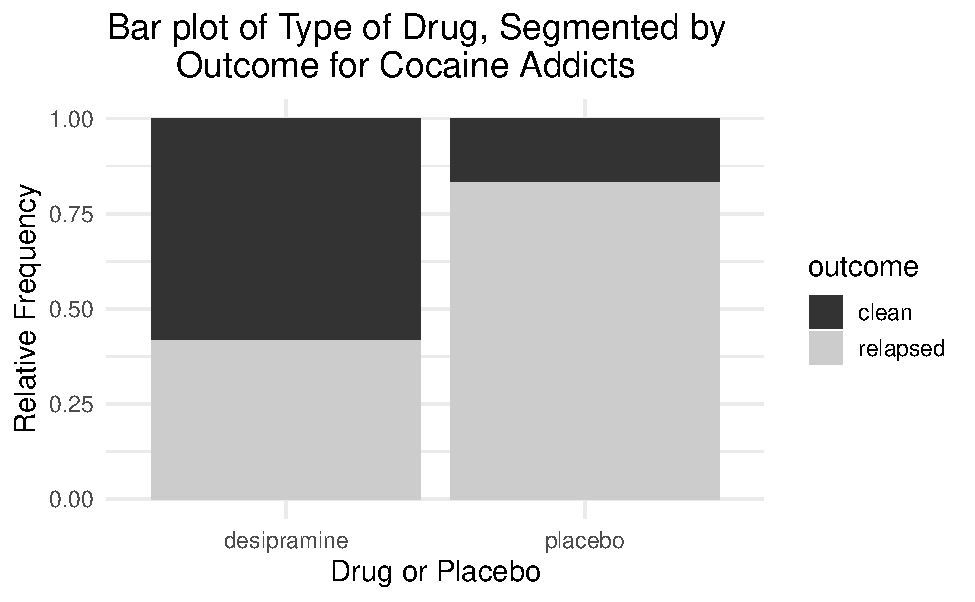
\includegraphics[width=0.7\linewidth]{08-LN09-two-cat-simulation_files/figure-latex/unnamed-chunk-3-1} \end{center}

\newpage

\hypertarget{hypothesis-testing-2}{%
\subsection*{Hypothesis Testing}\label{hypothesis-testing-2}}
\addcontentsline{toc}{subsection}{Hypothesis Testing}

Conditions:

\begin{itemize}
\tightlist
\item
  Independence: the response for one observational unit will not influence another observational unit
\end{itemize}

Null hypothesis assumes ``no effect'', ``no difference'', ``nothing interesting happening'', etc.

\rgi Always of form: ``parameter'' = null value

\(H_0:\)

\vspace{0.3in}

\(H_A:\)

\vspace{0.3in}

\begin{itemize}
\tightlist
\item
  Research question determines the alternative hypothesis.
\end{itemize}

Write the null and alternative hypotheses for the cocaine study:

In words:

\(H_0:\)

\vspace{0.5in}

\(H_A:\)

\vspace{0.5in}

In notation:

\(H_0:\)

\vspace{0.2in}

\(H_A:\)

\vspace{0.2in}

\hypertarget{simulation-based-method-2}{%
\subsubsection*{Simulation-based method}\label{simulation-based-method-2}}
\addcontentsline{toc}{subsubsection}{Simulation-based method}

\begin{itemize}
\item
  Simulate many samples assuming \(H_0: \pi_1 = \pi_2\)

  \begin{itemize}
  \item
    Write the response variable values on cards
  \item
    Mix the explanatory variable groups together
  \item
    Shuffle cards into two explanatory variable groups to represent the sample size in each group (\(n_1\) and \(n_2\))
  \item
    Calculate and plot the simulated difference in sample proportions from each simulation
  \item
    Repeat 1000 times (simulations) to create the null distribution
  \item
    Find the proportion of simulations at least as extreme as \(\hat{p}_1 - \hat{p}_2\)
  \end{itemize}
\end{itemize}

\newpage

\begin{Shaded}
\begin{Highlighting}[]
\FunctionTok{set.seed}\NormalTok{(}\DecValTok{216}\NormalTok{)}
\FunctionTok{two\_proportion\_test}\NormalTok{(}\AttributeTok{formula =}\NormalTok{ outcome}\SpecialCharTok{\textasciitilde{}}\NormalTok{drug, }\CommentTok{\# response \textasciitilde{} explanatory}
    \AttributeTok{data =}\NormalTok{ cocaine, }\CommentTok{\# Name of data set}
    \AttributeTok{first\_in\_subtraction =} \StringTok{"desipramine"}\NormalTok{, }\CommentTok{\# Order of subtraction: enter the name of Group 1}
    \AttributeTok{number\_repetitions =} \DecValTok{1000}\NormalTok{, }\CommentTok{\# Always use a minimum of 1000 repetitions}
    \AttributeTok{response\_value\_numerator =} \StringTok{"clean"}\NormalTok{, }\CommentTok{\# Define which outcome is a success}
    \AttributeTok{as\_extreme\_as =} \FloatTok{0.416}\NormalTok{, }\CommentTok{\# Calculated observed statistic (difference in sample proportions)}
    \AttributeTok{direction=}\StringTok{"greater"}\NormalTok{) }\CommentTok{\# Alternative hypothesis direction ("greater","less","two{-}sided")}
\end{Highlighting}
\end{Shaded}

\begin{center}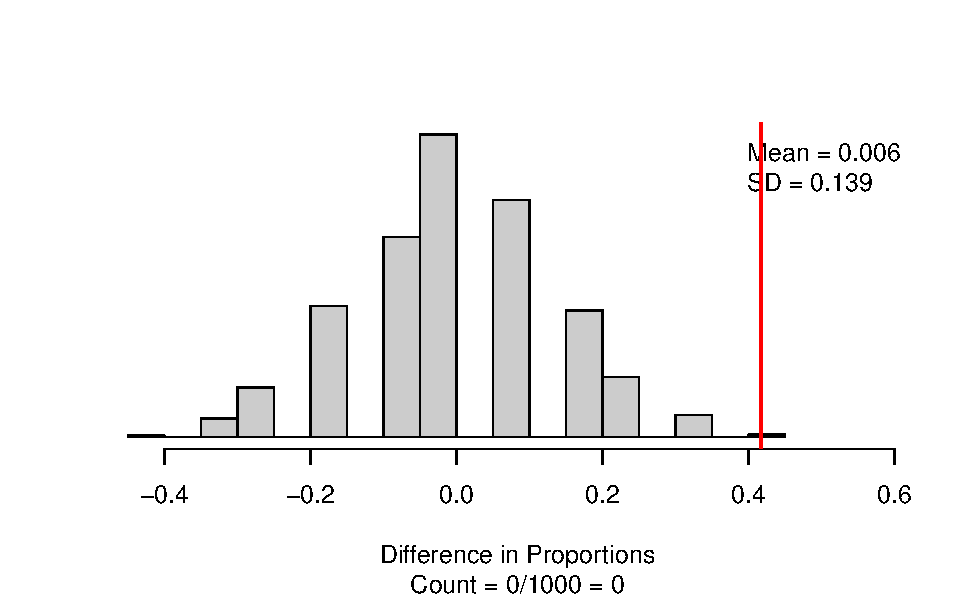
\includegraphics[width=0.7\linewidth]{08-LN09-two-cat-simulation_files/figure-latex/unnamed-chunk-4-1} \end{center}

Explain why the null distribution is centered at the value of zero:

\vspace{1in}

Interpretation of the p-value:

\begin{itemize}
\item
  Statement about probability or proportion of samples
\item
  Statistic (summary measure and value)
\item
  Direction of the alternative
\item
  Null hypothesis (in context)
\end{itemize}

\vspace{0.8in}

\newpage

Conclusion with scope of inference:

\begin{itemize}
\item
  Amount of evidence
\item
  Parameter of interest
\item
  Direction of the alternative hypothesis
\item
  Generalization
\item
  Causation
\end{itemize}

\vspace{0.8in}

\hypertarget{confidence-interval-2}{%
\subsection*{Confidence interval}\label{confidence-interval-2}}
\addcontentsline{toc}{subsection}{Confidence interval}

To estimate the difference in true proportion we will create a confidence interval.

\hypertarget{simulation-based-method-3}{%
\subsubsection*{Simulation-based method}\label{simulation-based-method-3}}
\addcontentsline{toc}{subsubsection}{Simulation-based method}

\begin{itemize}
\item
  Write the response variable values on cards
\item
  Keep explanatory variable groups separate
\item
  Sample with replacement \(n_1\) times in explanatory variable group 1 and \(n_2\) times in explanatory variable group 2
\item
  Calculate and plot the simulated difference in sample proportions from each simulation
\item
  Repeat 1000 times (simulations) to create the bootstrap distribution
\item
  Find the cut-offs for the middle X\% (confidence level) in a bootstrap distribution.
\end{itemize}

Returning to the cocaine example, we will estimate the difference in true proportion of cocaine addicts that stay clean for those on the desipramine and those on the placebo.

\begin{Shaded}
\begin{Highlighting}[]
\FunctionTok{set.seed}\NormalTok{(}\DecValTok{216}\NormalTok{)}
\FunctionTok{two\_proportion\_bootstrap\_CI}\NormalTok{(}\AttributeTok{formula =}\NormalTok{ outcome }\SpecialCharTok{\textasciitilde{}}\NormalTok{ drug, }
        \AttributeTok{data=}\NormalTok{cocaine, }\CommentTok{\# Name of data set}
        \AttributeTok{first\_in\_subtraction =} \StringTok{"desipramine"}\NormalTok{, }\CommentTok{\# Order of subtraction: enter the name of Group 1}
        \AttributeTok{response\_value\_numerator =} \StringTok{"clean"}\NormalTok{, }\CommentTok{\# Define which outcome is a success }
        \AttributeTok{number\_repetitions =} \DecValTok{1000}\NormalTok{, }\CommentTok{\# Always use a minimum of 1000 repetitions}
        \AttributeTok{confidence\_level =} \FloatTok{0.99}\NormalTok{) }\CommentTok{\# Enter the level of confidence as a decimal}
\end{Highlighting}
\end{Shaded}

\begin{center}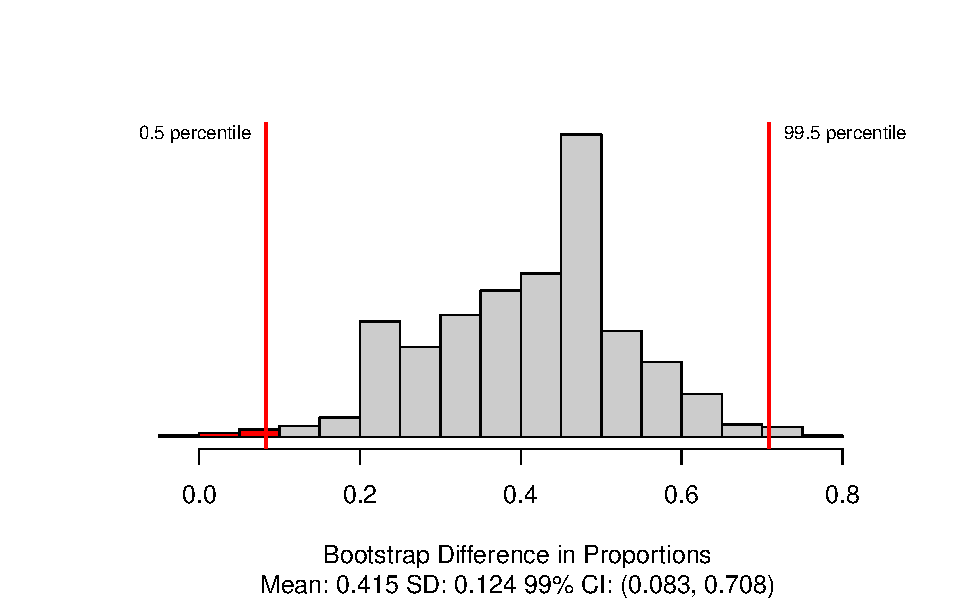
\includegraphics[width=0.7\linewidth]{08-LN09-two-cat-simulation_files/figure-latex/unnamed-chunk-5-1} \end{center}

Confidence interval interpretation:

\begin{itemize}
\item
  How confident you are (e.g., 90\%, 95\%, 98\%, 99\%)
\item
  Parameter of interest
\item
  Calculated interval
\item
  Order of subtraction when comparing two groups
\end{itemize}

\vspace{0.8in}

Does the confidence interval agree with the p-value?

\vspace{0.5in}

\newpage

\hypertarget{out-of-class-activity-week-8-the-good-samaritan-intro}{%
\section{Out-of-Class Activity Week 8: The Good Samaritan --- Intro}\label{out-of-class-activity-week-8-the-good-samaritan-intro}}

\setstretch{1}

\hypertarget{learning-outcomes-14}{%
\subsection{Learning outcomes}\label{learning-outcomes-14}}

\begin{itemize}
\item
  Given a research question involving two categorical variables, construct the null and alternative hypotheses
  in words and using appropriate statistical symbols.
\item
  Investigate the process of creating a null distribution for two categorical variables
\end{itemize}

\hypertarget{terminology-review-13}{%
\subsection{Terminology review}\label{terminology-review-13}}

In today's activity, we will use simulation-based methods to analyze two categorical variables. Some terms covered in this activity are:

\begin{itemize}
\item
  Conditional proportion
\item
  Null hypothesis
\item
  Alternative hypothesis
\end{itemize}

To review these concepts, see Chapter 15 in your textbook.

\hypertarget{the-good-samaritan}{%
\subsection{The Good Samaritan}\label{the-good-samaritan}}

Researchers at the Princeton University wanted to investigate influences on behavior (Darley and Batson 1973). The researchers randomly selected 67 students from the Princeton Theological Seminary to participate in a study. Only 47 students chose to participate in the study, and the data below includes 40 of those students (7 students were removed from the study for various reasons). As all participants were theology majors planning a career as a preacher, the expectation was that all would have a similar disposition when it comes to helping behavior. Each student was then shown a 5-minute presentation on the Good Samaritan, a parable in the Bible which emphasizes the importance of helping others. After the presentation, the students were told they needed to give a talk on the Good Samaritan parable at a building across campus. Half the students were told they were late for the presentation; the other half told they could take their time getting across campus (the condition was randomly assigned). On the way between buildings, an actor pretending to be a homeless person in distress asked the student for help. The researchers recorded whether the student helped the actor or not. The results of the study are shown in the table below. Do these data provide evidence that those in a hurry will be less likely to help people in need in this situation? Use the order of subtraction hurry -- no hurry.

\begin{center}
\begin{tabular}{|c|c|c|c|}\hline
& Hurry Condition & No Hurry Condition & Total \\ \hline
Helped Actor & 2 & 11 & 13 \\ \hline
Did Not Help Actor & 18 & 9 & 27 \\ \hline
Total & 20 & 20 & 40 \\ \hline
\end{tabular}
\end{center}

These counts can be found in R by using the \texttt{count()} function:

\begin{Shaded}
\begin{Highlighting}[]
\CommentTok{\# Read data set in}
\NormalTok{good }\OtherTok{\textless{}{-}} \FunctionTok{read.csv}\NormalTok{(}\StringTok{"https://math.montana.edu/courses/s216/data/goodsam.csv"}\NormalTok{) }
\NormalTok{good }\SpecialCharTok{\%\textgreater{}\%} \FunctionTok{group\_by}\NormalTok{(Condition) }\SpecialCharTok{\%\textgreater{}\%} \FunctionTok{count}\NormalTok{(Behavior)}
\end{Highlighting}
\end{Shaded}

\begin{verbatim}
#> # A tibble: 4 x 3
#> # Groups:   Condition [2]
#>   Condition Behavior     n
#>   <chr>     <chr>    <int>
#> 1 Hurry     Help         2
#> 2 Hurry     No help     18
#> 3 No hurry  Help        11
#> 4 No hurry  No help      9
\end{verbatim}

\hypertarget{vocabulary-review-1}{%
\subsubsection*{Vocabulary review}\label{vocabulary-review-1}}
\addcontentsline{toc}{subsubsection}{Vocabulary review}

\begin{enumerate}
\def\labelenumi{\arabic{enumi}.}
\tightlist
\item
  What is the name of the explanatory variable as it is written in the R output? What are its categories?
\end{enumerate}

\vspace{0.2in}

\begin{enumerate}
\def\labelenumi{\arabic{enumi}.}
\setcounter{enumi}{1}
\tightlist
\item
  What is the response variable in the R output? What are its categories?
\end{enumerate}

\vspace{0.2in}

\setstretch{1.5}

\begin{enumerate}
\def\labelenumi{\arabic{enumi}.}
\setcounter{enumi}{2}
\tightlist
\item
  Fill in the blanks with one answer from each set of parentheses: This is an\\
  \_\_\_\_\_\_\_\_\_\_\_\_\_\_\_\_ (experiment/observational study) because\\
  \_\_\_\_\_\_\_\_\_\_\_\_\_\_ (hurry or no hurry/help or no help) \_\_\_\_\_\_\_ (was/was not)\\
  randomly \_\_\_\_\_\_\_\_\_\_\_\_ (assigned/selected).
\end{enumerate}

\vspace{0.1in}

\begin{enumerate}
\def\labelenumi{\arabic{enumi}.}
\setcounter{enumi}{3}
\tightlist
\item
  Put an X in the box that represents the appropriate scope of inference for this study.
\end{enumerate}

\begin{center}
\begin{tabular}{|c|c|c|}\hline
& Study Type & \\ \hline
Selection of Cases & Randomized Experiment & Observational Study \\ \hline
Random Sample (no sampling bias) & & \\ \hline
Non Random Sample (sampling bias) & & \\ \hline
\end{tabular}
\end{center}

\setstretch{1}

\hypertarget{ask-a-research-question}{%
\subsubsection*{Ask a research question}\label{ask-a-research-question}}
\addcontentsline{toc}{subsubsection}{Ask a research question}

The research question as stated above is: Do these data provide evidence that those in a hurry will be less likely to help people in need in this situation? In order to set up our hypotheses, we need to express this research question in terms of parameters.

Remember, we define the parameter for a single categorical variable as the true proportion of observational units that are labeled as a ``success'' in the response variable.

\begin{enumerate}
\def\labelenumi{\arabic{enumi}.}
\setcounter{enumi}{4}
\item
  Write the two parameters of interest in context of the study.\\
  \vspace{1mm}

  \(\pi_{\text{hurry}}\) ---
  \vspace{0.5in}

  \(\pi_{\text{no hurry}}\) ---
  \vspace{0.5in}
\end{enumerate}

When comparing two groups, we assume the two parameters are equal in the null hypothesis---there is no association between the variables.

\begin{enumerate}
\def\labelenumi{\arabic{enumi}.}
\setcounter{enumi}{5}
\tightlist
\item
  Write the null hypothesis out in words using your answers to question 5.
\end{enumerate}

\vspace{0.6in}

\begin{enumerate}
\def\labelenumi{\arabic{enumi}.}
\setcounter{enumi}{6}
\tightlist
\item
  Based on the research question, fill in the appropriate sign for the alternative hypothesis (\(<\), \(>\), or \(\neq\)):
  \vspace{2mm}
\end{enumerate}

~~~~~~~~~~\(H_A: \pi_{\text{hurry}} -\pi_{\text{no hurry}}\) \_\_\_\_\_\_\_\_\_\_ 0

\hypertarget{summarize-and-visualize-the-data-1}{%
\subsubsection*{Summarize and visualize the data}\label{summarize-and-visualize-the-data-1}}
\addcontentsline{toc}{subsubsection}{Summarize and visualize the data}

\begin{Shaded}
\begin{Highlighting}[]
\NormalTok{good }\SpecialCharTok{\%\textgreater{}\%}
  \FunctionTok{ggplot}\NormalTok{(}\FunctionTok{aes}\NormalTok{(}\AttributeTok{x =}\NormalTok{ Condition, }\AttributeTok{fill =}\NormalTok{ Behavior))}\SpecialCharTok{+} \CommentTok{\#Enter the variables to plot}
  \FunctionTok{geom\_bar}\NormalTok{(}\AttributeTok{stat =} \StringTok{"count"}\NormalTok{, }\AttributeTok{position =} \StringTok{"fill"}\NormalTok{) }\SpecialCharTok{+}
  \FunctionTok{labs}\NormalTok{(}\AttributeTok{title =} \StringTok{"Segmented bar plot of Condition of Seminary }\SpecialCharTok{\textbackslash{}n}\StringTok{ Students by Behavior"}\NormalTok{, }\CommentTok{\#Title your plot}
       \AttributeTok{y =} \StringTok{"Relative Frequency"}\NormalTok{, }\CommentTok{\#y{-}axis label}
       \AttributeTok{x =} \StringTok{"Condition"}\NormalTok{) }\SpecialCharTok{+} \CommentTok{\#x{-}axis label}
  \FunctionTok{scale\_fill\_grey}\NormalTok{()}
\end{Highlighting}
\end{Shaded}

\begin{center}\includegraphics[width=0.8\linewidth]{08-OCA06-inference-2cat-simulation_files/figure-latex/unnamed-chunk-2-1} \end{center}

\begin{enumerate}
\def\labelenumi{\arabic{enumi}.}
\setcounter{enumi}{7}
\tightlist
\item
  Using the provided segmented bar plot, is there an association between whether a Seminary student helps the actor and condition assigned?
\end{enumerate}

\vspace{0.5in}

\begin{enumerate}
\def\labelenumi{\arabic{enumi}.}
\setcounter{enumi}{8}
\tightlist
\item
  Using the two-way table given in the introduction, calculate the conditional proportion of students in the hurry condition who helped the actor.
\end{enumerate}

\vspace{.3in}

\begin{enumerate}
\def\labelenumi{\arabic{enumi}.}
\setcounter{enumi}{9}
\tightlist
\item
  Using the two-way table given in the introduction, calculate the conditional proportion of students in the no hurry condition who helped the actor.
\end{enumerate}

\vspace{.3in}

\begin{enumerate}
\def\labelenumi{\arabic{enumi}.}
\setcounter{enumi}{10}
\tightlist
\item
  Calculate the summary statistic (difference in sample proportion) for this study. Use Hurry - No hurry as the order of subtraction.
\end{enumerate}

\vspace{0.4in}

\begin{enumerate}
\def\labelenumi{\arabic{enumi}.}
\setcounter{enumi}{11}
\tightlist
\item
  What is the notation used for the value calculated in question 11?
\end{enumerate}

\newpage

We will now simulate a \textbf{null distribution} of sample differences in proportions. The null distribution is created under the assumption the null hypothesis is true.

\begin{enumerate}
\def\labelenumi{\arabic{enumi}.}
\setcounter{enumi}{12}
\tightlist
\item
  First, let's think about how one simulation would be created on the null distribution using cards.
\end{enumerate}

\rgi How many cards would you need?
\vspace{0.1in}

\rgi What would be written on each card?

\vspace{0.5in}

\begin{enumerate}
\def\labelenumi{\arabic{enumi}.}
\setcounter{enumi}{13}
\tightlist
\item
  Next, we would mix the cards together and shuffle into two piles.
\end{enumerate}

\rgi How many cards would be in each pile?
\vspace{0.1in}

\rgi What would each pile represent?
\vspace{0.5in}

\begin{enumerate}
\def\labelenumi{\arabic{enumi}.}
\setcounter{enumi}{14}
\tightlist
\item
  Once we have one simulated sample, what would we calculate and plot on the null distribution? \emph{Hint}: What statistic are we calculating from the data?
\end{enumerate}

\vspace{0.8in}

The segmented bar plot below shows the relationship between the variables for one simulation assuming the null hypothesis is true.

\begin{center}\includegraphics[width=0.8\linewidth]{08-OCA06-inference-2cat-simulation_files/figure-latex/unnamed-chunk-3-1} \end{center}

\begin{enumerate}
\def\labelenumi{\arabic{enumi}.}
\setcounter{enumi}{15}
\tightlist
\item
  Compare the segmented bar plot for the simulated data to the previous segmented bar plot of the original data. Explain how the segmented bar plot of the simulated data reflects the null hypothesis.
\end{enumerate}

\vspace{1in}

\hypertarget{take-home-messages-12}{%
\subsection{Take-home messages}\label{take-home-messages-12}}

\begin{enumerate}
\def\labelenumi{\arabic{enumi}.}
\tightlist
\item
  When comparing two groups, we are looking at the difference between two parameters. In the null hypothesis, we assume the two parameters are equal, or that there is no difference between the two proportions.
\end{enumerate}

\begin{enumerate}
\def\labelenumi{\arabic{enumi}.}
\setcounter{enumi}{1}
\tightlist
\item
  To create one simulated sample on the null distribution for a difference in sample proportions, label \(n_1 + n_2\) cards with the response variable outcomes from the original data. Mix cards together and shuffle into two new groups of sizes \(n_1\) and \(n_2\), representing the explanatory variable groups. Calculate and plot the difference in proportion of successes.
\end{enumerate}

\hypertarget{additional-notes-12}{%
\subsection{Additional notes}\label{additional-notes-12}}

Use this space to summarize your thoughts and take additional notes on today's activity and material covered.

\newpage

\hypertarget{activity-8-the-good-samaritan-continued-simulation-based-hypothesis-test-confidence-interval}{%
\section{Activity 8: The Good Samaritan (continued) --- Simulation-based Hypothesis Test \& Confidence Interval}\label{activity-8-the-good-samaritan-continued-simulation-based-hypothesis-test-confidence-interval}}

\setstretch{1}

\hypertarget{learning-outcomes-15}{%
\subsection{Learning outcomes}\label{learning-outcomes-15}}

\begin{itemize}
\item
  Identify the parameter of interest for a difference in proportions.
\item
  Describe and perform a simulation-based hypothesis test for a difference in proportions
\item
  Interpret and evaluate a p-value for a simulation-based hypothesis test for a difference in proportions.
\item
  Create and interpret a simulation-based confidence interval for a difference in proportions.
\end{itemize}

\hypertarget{terminology-review-14}{%
\subsection{Terminology review}\label{terminology-review-14}}

In today's activity, we will use simulation methods to estimate the difference in two proportions. Some terms covered in this activity are:

\begin{itemize}
\item
  Hypothesis test
\item
  P-value
\item
  Parameter of interest
\item
  Bootstrapping
\item
  Confidence interval
\item
  Types of errors
\end{itemize}

To review these concepts, see Chapter 15 in your textbook.

\hypertarget{the-good-samaritan-1}{%
\subsection{The Good Samaritan}\label{the-good-samaritan-1}}

In the out of class activity, we began a test of significance to see if people in a hurry are less likely to help those in need. Today we will use RStudio to continue to assess this research question.

Researchers at the Princeton University wanted to investigate influences on behavior (Darley and Batson 1973). The researchers randomly selected 67 students from the Princeton Theological Seminary to participate in a study. Only 47 students chose to participate in the study, and the data below includes 40 of those students (7 students were removed from the study for various reasons). As all participants were theology majors planning a career as a preacher, the expectation was that all would have a similar disposition when it comes to helping behavior. Each student was then shown a 5-minute presentation on the Good Samaritan, a parable in the Bible which emphasizes the importance of helping others. After the presentation, the students were told they needed to give a talk on the Good Samaritan parable at a building across campus. Half the students were told they were late for the presentation; the other half told they could take their time getting across campus (the condition was randomly assigned). On the way between buildings, an actor pretending to be a homeless person in distress asked the student for help. The researchers recorded whether the student helped the actor or not. The results of the study are shown in the table below. Do these data provide evidence that those in a hurry will be less likely to help people in need in this situation? Use the order of subtraction hurry -- no hurry.

\begin{longtable}[]{@{}llll@{}}
\toprule\noalign{}
& Hurry Condition & No Hurry Condition & Total \\
\midrule\noalign{}
\endhead
\bottomrule\noalign{}
\endlastfoot
Helped Actor & 2 & 11 & 13 \\
Did Not Help Actor & 18 & 9 & 27 \\
Total & 20 & 20 & 40 \\
\end{longtable}

\newpage

\begin{enumerate}
\def\labelenumi{\arabic{enumi}.}
\tightlist
\item
  Simulate one sample assuming the null hypothesis is true using the cards provided by your instructor. Write down the value of the simulated statistic. How does the value of your group's simulated statistic compare to the other groups at your table? Are the simulated values closer to the null value of zero than the actual calculated difference in proportions?
\end{enumerate}

\vspace{1in}

To create the null distribution of differences in sample proportions, we will use the \texttt{two\_proportion\_test()} function in R (in the \texttt{catstats} package). We will need to enter the response variable name and the explanatory variable name for the formula, the data set name (identified above as \texttt{good}), the outcome for the explanatory variable that is first in subtraction, number of repetitions, the outcome for the response variable that is a success (what the numerator counts when calculating a sample proportion), and the direction of the alternative hypothesis.

The response variable name is \texttt{Behavior} and the explanatory variable name is \texttt{Condition}.

\begin{enumerate}
\def\labelenumi{\arabic{enumi}.}
\setcounter{enumi}{1}
\tightlist
\item
  What inputs should be entered for each of the following to create the simulation?
  \vspace{1mm}
\end{enumerate}

\begin{itemize}
\tightlist
\item
  First in subtraction (What is the outcome for the explanatory variable that is used as first in the order of subtraction? \texttt{"Hurry"} or \texttt{"No\ hurry"}):
\end{itemize}

\vspace{.15in}

\begin{itemize}
\tightlist
\item
  Number of repetitions:
\end{itemize}

\vspace{.15in}

\begin{itemize}
\tightlist
\item
  Response value numerator (What is the outcome for the response variable that is considered a success? \texttt{"Help"} or \texttt{"No\ help"}):
\end{itemize}

\vspace{.15in}

\begin{itemize}
\tightlist
\item
  As extreme as (enter the value for the sample difference in proportions):
\end{itemize}

\vspace{.15in}

\begin{itemize}
\tightlist
\item
  Direction (\texttt{"greater"}, \texttt{"less"}, or \texttt{"two-sided"}):
\end{itemize}

\vspace{.15in}

Using the R script file for this activity, enter your answers for question 16 in place of the \texttt{xx}'s to produce the null distribution with 1000 simulations; highlight and run lines 1--16.

\begin{Shaded}
\begin{Highlighting}[]
\FunctionTok{two\_proportion\_test}\NormalTok{(}\AttributeTok{formula =}\NormalTok{ Behavior}\SpecialCharTok{\textasciitilde{}}\NormalTok{Condition, }\CommentTok{\# response \textasciitilde{} explanatory}
    \AttributeTok{data =}\NormalTok{ good, }\CommentTok{\# Name of data set}
    \AttributeTok{first\_in\_subtraction =} \StringTok{"xx"}\NormalTok{, }\CommentTok{\# Order of subtraction: enter the name of Group 1}
    \AttributeTok{number\_repetitions =} \DecValTok{1000}\NormalTok{, }\CommentTok{\# Always use a minimum of 1000 repetitions}
    \AttributeTok{response\_value\_numerator =} \StringTok{"xx"}\NormalTok{, }\CommentTok{\# Define which outcome is a success}
    \AttributeTok{as\_extreme\_as =}\NormalTok{ xx, }\CommentTok{\# Calculated observed statistic (difference in sample proportions)}
    \AttributeTok{direction=}\StringTok{"xx"}\NormalTok{) }\CommentTok{\# Alternative hypothesis direction ("greater","less","two{-}sided")}
\end{Highlighting}
\end{Shaded}

\begin{enumerate}
\def\labelenumi{\arabic{enumi}.}
\setcounter{enumi}{2}
\tightlist
\item
  Sketch the null distribution created here.
\end{enumerate}

\vspace{1.5in}

\begin{enumerate}
\def\labelenumi{\arabic{enumi}.}
\setcounter{enumi}{3}
\tightlist
\item
  What value is the null distribution centered around? Explain why this makes sense.
\end{enumerate}

\vspace{.8in}

\begin{enumerate}
\def\labelenumi{\arabic{enumi}.}
\setcounter{enumi}{4}
\tightlist
\item
  What is the value of the p-value? \emph{Remember}: This is the value given at the bottom of the null distribution.
\end{enumerate}

\vspace{0.2in}

\begin{enumerate}
\def\labelenumi{\arabic{enumi}.}
\setcounter{enumi}{5}
\tightlist
\item
  Interpret the p-value in context of the study.
\end{enumerate}

\vspace{1in}

\begin{enumerate}
\def\labelenumi{\arabic{enumi}.}
\setcounter{enumi}{6}
\tightlist
\item
  How much evidence does the p-value provide against the null hypothesis? \emph{Hint}: Refer to the guidelines given in Week 6.
\end{enumerate}

\vspace{0.4in}

\begin{enumerate}
\def\labelenumi{\arabic{enumi}.}
\setcounter{enumi}{7}
\tightlist
\item
  Do you expect the null value to be in a 99\% confidence interval? Explain your answer.
\end{enumerate}

\vspace{0.6in}

\hypertarget{use-statistical-analysis-methods-to-draw-inferences-from-the-data-2}{%
\subsubsection*{Use statistical analysis methods to draw inferences from the data}\label{use-statistical-analysis-methods-to-draw-inferences-from-the-data-2}}
\addcontentsline{toc}{subsubsection}{Use statistical analysis methods to draw inferences from the data}

In this part of the activity, we will estimate the difference in true proportion of people who will help others for those in the hurry condition and those not in the hurry condition by finding a confidence interval.

\begin{enumerate}
\def\labelenumi{\arabic{enumi}.}
\setcounter{enumi}{8}
\tightlist
\item
  Write the parameter of interest in context of the study. Use proper notation.
\end{enumerate}

\vspace{1in}

We will use the \texttt{two\_proportion\_bootstrap\_CI()} function in R (in the \texttt{catstats} package) to simulate the bootstrap distribution of differences in sample proportions and calculate a confidence interval. We will need to enter the response variable name and the explanatory variable name for the formula, the data set name (identified above as \texttt{good}), the outcome for the explanatory variable that is first in subtraction, number of repetitions, the outcome for the response variable that is a success (what the numerator counts when calculating a sample proportion), and the confidence level as a decimal.

\newpage

The response variable name is \texttt{Behavior} and the explanatory variable name is \texttt{Condition}.

\begin{enumerate}
\def\labelenumi{\arabic{enumi}.}
\setcounter{enumi}{9}
\tightlist
\item
  What values should be entered for each of the following into the simulation to create a 99\% confidence interval?
  \vspace{.5mm}
\end{enumerate}

\begin{itemize}
\tightlist
\item
  First in subtraction (What is the outcome for the explanatory variable that is used as first in the order of subtraction? \texttt{"Hurry"} or \texttt{"No\ hurry"}):
\end{itemize}

\vspace{.15in}

\begin{itemize}
\tightlist
\item
  Response value numerator (What is the outcome for the response variable that is considered a success? \texttt{"Help"} or \texttt{"No\ help"}):
\end{itemize}

\vspace{.15in}

\begin{itemize}
\tightlist
\item
  Number of repetitions:
\end{itemize}

\vspace{.15in}

\begin{itemize}
\tightlist
\item
  Confidence level (entered as a decimal):
\end{itemize}

\vspace{.15in}

Using the R script file for this activity, enter your answers for question 7 in place of the \texttt{xx}'s to produce the bootstrap distribution with 1000 simulations; highlight and run lines 16--21.

\begin{Shaded}
\begin{Highlighting}[]
\FunctionTok{two\_proportion\_bootstrap\_CI}\NormalTok{(}\AttributeTok{formula =}\NormalTok{ Behavior }\SpecialCharTok{\textasciitilde{}}\NormalTok{ Condition, }
        \AttributeTok{data=}\NormalTok{good, }\CommentTok{\# Name of data set}
        \AttributeTok{first\_in\_subtraction =} \StringTok{"xx"}\NormalTok{, }\CommentTok{\# Order of subtraction: enter the name of Group 1}
        \AttributeTok{response\_value\_numerator =} \StringTok{"xx"}\NormalTok{, }\CommentTok{\# Define which outcome is a success }
        \AttributeTok{number\_repetitions =} \DecValTok{1000}\NormalTok{, }\CommentTok{\# Always use a minimum of 1000 repetitions}
        \AttributeTok{confidence\_level =}\NormalTok{ xx) }\CommentTok{\# Enter the level of confidence as a decimal}
\end{Highlighting}
\end{Shaded}

\begin{enumerate}
\def\labelenumi{\arabic{enumi}.}
\setcounter{enumi}{10}
\tightlist
\item
  Where is the bootstrap distribution centered? Explain why.
\end{enumerate}

\vspace{0.8in}

\begin{enumerate}
\def\labelenumi{\arabic{enumi}.}
\setcounter{enumi}{11}
\tightlist
\item
  Report the bootstrap 99\% confidence interval.
\end{enumerate}

\vspace{0.4in}

\begin{enumerate}
\def\labelenumi{\arabic{enumi}.}
\setcounter{enumi}{12}
\tightlist
\item
  What percentile of the bootstrap distribution does the upper value of the confidence interval represent?
\end{enumerate}

\vspace{0.3in}

\begin{enumerate}
\def\labelenumi{\arabic{enumi}.}
\setcounter{enumi}{13}
\tightlist
\item
  Interpret the 99\% confidence interval in context of the problem.
\end{enumerate}

\vspace{1in}

\begin{enumerate}
\def\labelenumi{\arabic{enumi}.}
\setcounter{enumi}{14}
\tightlist
\item
  Write a conclusion to the test.
\end{enumerate}

\vspace{0.8in}

\newpage

\hypertarget{take-home-messages-13}{%
\subsection{Take-home messages}\label{take-home-messages-13}}

\begin{enumerate}
\def\labelenumi{\arabic{enumi}.}
\item
  We use the same guidelines for the strength of evidence as we did in Activity 6A.
\item
  To create one simulated sample on the bootstrap distribution for a difference in sample proportions, label \(n_1 + n_2\) cards with the outcomes for the original responses. Keep groups separate and randomly draw with replacement \(n_1\) times from group 1 and \(n_2\) times from group 2. Calculate and plot the resampled difference in the proportion of successes.
\item
  If the null value is not contained in a 99\% confidence interval, then there is evidence against the null hypothesis and the p-value is less than the significance level of 0.01.
\end{enumerate}

\hypertarget{additional-notes-13}{%
\subsection{Additional notes}\label{additional-notes-13}}

Use this space to summarize your thoughts and take additional notes on today's activity and material covered.

\newpage

\hypertarget{week-8-lab-poisonous-mushrooms}{%
\section{Week 8 Lab: Poisonous Mushrooms}\label{week-8-lab-poisonous-mushrooms}}

\setstretch{1}

\hypertarget{learning-outcomes-16}{%
\subsection{Learning outcomes}\label{learning-outcomes-16}}

\begin{itemize}
\item
  Given a research question involving two categorical variables, construct the null and alternative hypotheses
  in words and using appropriate statistical symbols.
\item
  Describe and perform a simulation-based hypothesis test for a difference in proportions.
\item
  Interpret and evaluate a p-value for a simulation-based hypothesis test for a difference in proportions.
\item
  Interpret and evaluate a confidence interval for a simulation-based confidence interval for a difference in proportions.
\end{itemize}

\hypertarget{poisonous-mushrooms}{%
\subsection{Poisonous Mushrooms}\label{poisonous-mushrooms}}

Wild mushrooms, such as chanterelles or morels, are delicious, but eating wild mushrooms carries the risk of accidental poisoning. Even a single bite of the wrong mushroom can be enough to cause fatal poisoning. An amateur mushroom hunter is interested in finding an easy rule to differentiate poisonous and edible mushrooms. They think that the mushroom's gills (the part which holds and releases spores) might be related to a mushroom's edibility. They used a data set of 8124 mushrooms and their descriptions. For each mushroom, the data set includes whether it is edible (e) or poisonous (p) and the size of the gills (broad (b) or narrow (n)). Is there evidence gill size is associated with whether a mushroom is poisonous? PLEASE NOTE: According to The Audubon Society Field Guide to North American Mushrooms, there is no simple rule for determining the edibility of a mushroom; no rule like ``leaflets three, let it be'\,' for Poisonous Oak and Ivy.

\begin{itemize}
\item
  Upload and open the R script file for Week 8 lab. Upload and import the csv file, \texttt{mushrooms\_edibility}.
\item
  Enter the name of the data set (see the environment tab) for datasetname in the R script file in line 8.
\item
  Highlight and run lines 1--9 to get the counts for each combination of categories.
\end{itemize}

\begin{Shaded}
\begin{Highlighting}[]
\NormalTok{mushrooms }\OtherTok{\textless{}{-}}\NormalTok{ datasetname }\CommentTok{\# Read data set in}
\NormalTok{mushrooms }\SpecialCharTok{\%\textgreater{}\%} \FunctionTok{group\_by}\NormalTok{(gill\_size) }\SpecialCharTok{\%\textgreater{}\%} \FunctionTok{count}\NormalTok{(edibility) }\CommentTok{\#finds the counts in each group}
\end{Highlighting}
\end{Shaded}

\begin{enumerate}
\def\labelenumi{\arabic{enumi}.}
\tightlist
\item
  What is the explanatory variable? How are the two levels of the explanatory variable written in the data set?
\end{enumerate}

\vspace{0.5in}

\begin{enumerate}
\def\labelenumi{\arabic{enumi}.}
\setcounter{enumi}{1}
\tightlist
\item
  What is the response variable? How are the two levels of the response variable written in the data set?
\end{enumerate}

\vspace{0.5in}

\begin{enumerate}
\def\labelenumi{\arabic{enumi}.}
\setcounter{enumi}{2}
\tightlist
\item
  Fill in the following two-way table using the R output.
\end{enumerate}

\begin{center}
\begin{tabular}{|c|c|c|c|}\hline
& \multicolumn{2}{|c|}{\textbf{Gill Size}} & \\ \hline
\textbf{Edibility} & \hspace{0.35in} Broad (b) \hspace{0.35in} & \hspace{0.35in} Narrow (n) \hspace{0.35in} & \hspace{0.35in} Total \hspace{0.35in} \\ \hline
 Poisonous (p) & & & \\ 
 & & & \\ \hline
Edible (e) & & & \\ 
 & & & \\ \hline
 Total & & & \\ 
 & & & \\ \hline
\end{tabular}
\end{center}

\newpage

\begin{enumerate}
\def\labelenumi{\arabic{enumi}.}
\setcounter{enumi}{3}
\tightlist
\item
  Write the parameter of interest in words, in context of the study.
\end{enumerate}

\vspace{1in}

\begin{enumerate}
\def\labelenumi{\arabic{enumi}.}
\setcounter{enumi}{4}
\tightlist
\item
  \textbf{Calculate the difference in proportion of mushrooms that are poisonous for broad gill mushrooms and narrow gill mushrooms. Use broad - narrow for the order of subtraction. Use appropriate notation.}
\end{enumerate}

\vspace{0.8in}

\begin{enumerate}
\def\labelenumi{\arabic{enumi}.}
\setcounter{enumi}{5}
\tightlist
\item
  Write the null hypothesis for this study in notation.
\end{enumerate}

\vspace{0.25in}

\begin{enumerate}
\def\labelenumi{\arabic{enumi}.}
\setcounter{enumi}{6}
\tightlist
\item
  \textbf{Using the research question, write the alternative hypothesis in words.}
\end{enumerate}

\vspace{1in}

\begin{itemize}
\tightlist
\item
  Fill in the missing values/names in the R script file for the \texttt{two-proportion\_test} function to create the null distribution and find the p-value for the test.
\end{itemize}

\begin{Shaded}
\begin{Highlighting}[]
\FunctionTok{two\_proportion\_test}\NormalTok{(}\AttributeTok{formula =}\NormalTok{ response}\SpecialCharTok{\textasciitilde{}}\NormalTok{explanatory, }\CommentTok{\# response \textasciitilde{} explanatory}
    \AttributeTok{data=}\NormalTok{ mushrooms, }\CommentTok{\# Name of data set}
    \AttributeTok{first\_in\_subtraction =} \StringTok{"xx"}\NormalTok{, }\CommentTok{\# Order of subtraction: enter the name of Group 1}
    \AttributeTok{number\_repetitions =} \DecValTok{1000}\NormalTok{, }\CommentTok{\# Always use a minimum of 1000 repetitions}
    \AttributeTok{response\_value\_numerator =} \StringTok{"xx"}\NormalTok{, }\CommentTok{\# Define which outcome is a success }
    \AttributeTok{as\_extreme\_as =}\NormalTok{ xx, }\CommentTok{\# Calculated observed statistic (difference in sample proportions)}
    \AttributeTok{direction=}\StringTok{"xx"}\NormalTok{) }\CommentTok{\# Alternative hypothesis direction ("greater","less","two{-}sided")}
\end{Highlighting}
\end{Shaded}

\begin{enumerate}
\def\labelenumi{\arabic{enumi}.}
\setcounter{enumi}{7}
\tightlist
\item
  Report the p-value for the study.
\end{enumerate}

\vspace{0.2in}

\begin{enumerate}
\def\labelenumi{\arabic{enumi}.}
\setcounter{enumi}{8}
\tightlist
\item
  \textbf{Do you expect that a 90\% confidence interval would contain the null value of zero? Explain your answer.}
\end{enumerate}

\vspace{0.8in}

\newpage

\begin{itemize}
\item
  Fill in the missing values/names in the R script file in the two\_proportion\_bootstrap\_CI function to create a simulation 90\% confidence interval.
\item
  \textbf{Upload a copy of the bootstrap distribution to Gradescope.}
\end{itemize}

\begin{Shaded}
\begin{Highlighting}[]
\FunctionTok{two\_proportion\_bootstrap\_CI}\NormalTok{(}\AttributeTok{formula =}\NormalTok{ response}\SpecialCharTok{\textasciitilde{}}\NormalTok{explanatory, }
         \AttributeTok{data=}\NormalTok{mushrooms, }\CommentTok{\# Name of data set}
         \AttributeTok{first\_in\_subtraction =} \StringTok{"xx"}\NormalTok{, }\CommentTok{\# Order of subtraction: enter the name of Group 1}
         \AttributeTok{response\_value\_numerator =} \StringTok{"xx"}\NormalTok{, }\CommentTok{\# Define which outcome is a success }
         \AttributeTok{number\_repetitions =} \DecValTok{1000}\NormalTok{, }\CommentTok{\# Always use a minimum of 1000 repetitions}
         \AttributeTok{confidence\_level =}\NormalTok{ xx) }\CommentTok{\# Enter the level of confidence as a decimal}
\end{Highlighting}
\end{Shaded}

\begin{enumerate}
\def\labelenumi{\arabic{enumi}.}
\setcounter{enumi}{9}
\tightlist
\item
  Report the 90\% confidence interval.
\end{enumerate}

\vspace{0.2in}

\begin{enumerate}
\def\labelenumi{\arabic{enumi}.}
\setcounter{enumi}{10}
\tightlist
\item
  Write a paragraph summarizing the results of the study as if writing a press release. Be sure to describe:
\end{enumerate}

\begin{itemize}
\item
  Summary statistic and interpretation

  \begin{itemize}
  \item
    Summary measure (in context)
  \item
    Value of the statistic
  \item
    Order of subtraction when comparing two groups
  \end{itemize}
\item
  P-value and interpretation

  \begin{itemize}
  \item
    Statement about probability or proportion of samples
  \item
    Statistic (summary measure and value)
  \item
    Direction of the alternative
  \item
    Null hypothesis (in context)
  \end{itemize}
\item
  Confidence interval and interpretation

  \begin{itemize}
  \item
    How confident you are (e.g., 90\%, 95\%, 98\%, 99\%)
  \item
    Parameter of interest
  \item
    Calculated interval
  \item
    Order of subtraction when comparing two groups
  \end{itemize}
\item
  Conclusion (written to answer the research question)

  \begin{itemize}
  \item
    Amount of evidence
  \item
    Parameter of interest
  \item
    Direction of the alternative hypothesis
  \end{itemize}
\item
  Scope of inference

  \begin{itemize}
  \item
    To what group of observational units do the results apply (target population or observational units similar to the sample)?
  \item
    What type of inference is appropriate (causal or non-causal)?
  \end{itemize}
\end{itemize}

\textbf{Upload your group's confidence interval interpretation and conclusion to Gradescope.}

\newpage

Paragraph:

\newpage

\hypertarget{inference-for-two-categorical-variables-theory-based-methods}{%
\chapter{Inference for Two Categorical Variables: Theory-based Methods}\label{inference-for-two-categorical-variables-theory-based-methods}}

\hypertarget{lecture-notes-week-9-theoretical-inference-for-two-categorical-variables}{%
\section{Lecture Notes Week 9: Theoretical Inference for Two Categorical Variables}\label{lecture-notes-week-9-theoretical-inference-for-two-categorical-variables}}

\setstretch{1}

\hypertarget{hypothesis-testing-using-theory-based-methods}{%
\subsection*{Hypothesis testing using theory-based methods}\label{hypothesis-testing-using-theory-based-methods}}
\addcontentsline{toc}{subsection}{Hypothesis testing using theory-based methods}

Conditions for inference using theory-based methods for two categorical variables:

\begin{itemize}
\tightlist
\item
  Independence: the response for one observational unit will not influence another observational unit
\end{itemize}

\vspace{0.2in}

\begin{itemize}
\tightlist
\item
  Large enough sample size:
\end{itemize}

\vspace{1in}

\begin{itemize}
\item
  Calculate the standardized statistic
\item
  Find the area under the standard normal distribution at least as extreme as the standardized statistic
\end{itemize}

Equation for the standard error of the difference in sample proportions assuming the null hypothesis is true:

\vspace{0.8in}

\setstretch{1.5}

\begin{itemize}
\tightlist
\item
  This value measures how far each possible sample difference in \_\_\_\_\_\_\_\_\_\_\_\_\_ is from the \_\_\_\_\_\_\_\_\_ value, on average.
\end{itemize}

\setstretch{1}

Equation for the standardized difference in sample proportions:

\vspace{0.8in}

\setstretch{1.5}

\begin{itemize}
\tightlist
\item
  This value measures how many \_\_\_\_\_\_\_\_\_\_\_\_\_ deviations the sample difference in \_\_\_\_\_\_\_\_\_\_\_\_\_ is above/below the \_\_\_\_\_\_\_\_\_\_ value.
\end{itemize}

\setstretch{1}

Example for class discussion: In the week 3 Lab, we investigated data on higher education institutions in the United States, collected by the Integrated Postsecondary Education Data System (IPEDS) for the National Center for Education Statistics (NCES) (Education Statistics 2018). A random sample of 2900+ higher education institutions in the United States was collected in 2018. Two variables measured on this data set is whether the institution is a land grant university and whether the institution offers tenure. Does the proportion of universities that offer tenure differ between land grant and non-land-grant institutions?

Are the conditions met to analyze the university data using theory-based methods?

\vspace{0.8in}

\begin{Shaded}
\begin{Highlighting}[]
\NormalTok{IPED }\OtherTok{\textless{}{-}}\FunctionTok{read.csv}\NormalTok{(}\StringTok{"https://math.montana.edu/courses/s216/data/IPEDS\_2018.csv"}\NormalTok{)}

\NormalTok{IPEDS }\OtherTok{\textless{}{-}}\NormalTok{ IPED }\SpecialCharTok{\%\textgreater{}\%}
    \FunctionTok{drop\_na}\NormalTok{(Tenure)}

\NormalTok{IPEDS }\SpecialCharTok{\%\textgreater{}\%} \CommentTok{\# Data set piped into...}
    \FunctionTok{ggplot}\NormalTok{(}\FunctionTok{aes}\NormalTok{(}\AttributeTok{x =}\NormalTok{ LandGrant, }\AttributeTok{fill =}\NormalTok{ Tenure)) }\SpecialCharTok{+}   \CommentTok{\# This specifies the variables}
  \FunctionTok{geom\_bar}\NormalTok{(}\AttributeTok{stat =} \StringTok{"count"}\NormalTok{, }\AttributeTok{position =} \StringTok{"fill"}\NormalTok{) }\SpecialCharTok{+}  \CommentTok{\# Tell it to make a stacked bar plot}
  \FunctionTok{labs}\NormalTok{(}\AttributeTok{title =} \StringTok{"Segmented Bar Plot of Tenure Availability }
\StringTok{       by Type of Institution for Higher Ed Institutions"}\NormalTok{,  }
       \CommentTok{\# Make sure to title your plot }
       \AttributeTok{x =} \StringTok{"Land Grant"}\NormalTok{,   }\CommentTok{\# Label the x axis}
       \AttributeTok{y =} \StringTok{""}\NormalTok{) }\SpecialCharTok{+} \CommentTok{\# Remove y axis label }
    \FunctionTok{scale\_fill\_grey}\NormalTok{()}

\NormalTok{IPEDS }\SpecialCharTok{\%\textgreater{}\%} \FunctionTok{group\_by}\NormalTok{(LandGrant) }\SpecialCharTok{\%\textgreater{}\%} \FunctionTok{count}\NormalTok{(Tenure)}
\CommentTok{\#\textgreater{} \# A tibble: 4 x 3}
\CommentTok{\#\textgreater{} \# Groups:   LandGrant [2]}
\CommentTok{\#\textgreater{}   LandGrant Tenure     n}
\CommentTok{\#\textgreater{}   \textless{}chr\textgreater{}     \textless{}chr\textgreater{}  \textless{}int\textgreater{}}
\CommentTok{\#\textgreater{} 1 No        No       976}
\CommentTok{\#\textgreater{} 2 No        Yes     1829}
\CommentTok{\#\textgreater{} 3 Yes       No        31}
\CommentTok{\#\textgreater{} 4 Yes       Yes       72}
\end{Highlighting}
\end{Shaded}

\begin{center}\includegraphics[width=0.7\linewidth]{09-LN010-two-cat-theory_files/figure-latex/unnamed-chunk-1-1} \end{center}

What is the explanatory variable?

\vspace{0.2in}

What is the response variable?

\vspace{0.2in}

Write the parameter of interest:

\vspace{0.8in}

Hypotheses:

In notation:

\(H_0:\)

\vspace{0.2in}

\(H_A:\)

\vspace{0.2in}

In words:

\(H_0:\)

\vspace{0.6in}

\(H_A:\)

\vspace{0.6in}

Report the summary statistic:

\vspace{0.8in}

Calculate the standardized difference in sample proportion of higher education institutions that offer tenure between land grant universities and non-land grant universities.

\begin{itemize}
\tightlist
\item
  First calculate the standard error of the difference in proportion assuming the null hypothesis is true
\end{itemize}

\vspace{0.5in}

\begin{itemize}
\tightlist
\item
  Then calculate the Z score
\end{itemize}

\vspace{0.5in}

\begin{center}\includegraphics[width=0.5\linewidth]{09-LN010-two-cat-theory_files/figure-latex/standNormc-1} \end{center}

Interpret the standardized statistic

\vspace{0.5in}

To find the p-value, find the area under the standard normal distribution at the standardized statistic and more extreme.

\begin{Shaded}
\begin{Highlighting}[]
\FunctionTok{pnorm}\NormalTok{(}\FloatTok{0.985}\NormalTok{, }\AttributeTok{lower.tail =} \ConstantTok{FALSE}\NormalTok{)}\SpecialCharTok{*}\DecValTok{2}
\CommentTok{\#\textgreater{} [1] 0.3246241}
\end{Highlighting}
\end{Shaded}

Interpretation of the p-value:

\begin{itemize}
\item
  Statement about probability or proportion of samples
\item
  Statistic (summary measure and value)
\item
  Direction of the alternative
\item
  Null hypothesis (in context)
\end{itemize}

\vspace{0.8in}

Conclusion with scope of inference:

\begin{itemize}
\item
  Amount of evidence
\item
  Parameter of interest
\item
  Direction of the alternative hypothesis
\item
  Generalization
\item
  Causation
\end{itemize}

\vspace{0.6in}

\newpage

\hypertarget{confidence-interval-3}{%
\subsection*{Confidence interval}\label{confidence-interval-3}}
\addcontentsline{toc}{subsection}{Confidence interval}

\begin{itemize}
\item
  Estimate the \_\_\_\_\_\_\_\_\_\_\_\_\_\_\_ in true \_\_\_\_\_\_\_\_\_\_\_\_\_\_\_
\item
  \(CI = \text{statistic} \pm \text{margin of error}\)
\end{itemize}

\hypertarget{theory-based-method-for-a-two-categorical-variables}{%
\subsubsection*{Theory-based method for a two categorical variables}\label{theory-based-method-for-a-two-categorical-variables}}
\addcontentsline{toc}{subsubsection}{Theory-based method for a two categorical variables}

\begin{itemize}
\tightlist
\item
  \(CI = \hat{p}_1-\hat{p}_2 \pm (z^* \times SE(\hat{p}_1-\hat{p}_2))\)
\end{itemize}

\setstretch{1.5}

\begin{itemize}
\tightlist
\item
  When creating a confidence interval, we no longer assume the \_\_\_\_\_\_\_\_\_\_\_\_\_ hypothesis is true. Use the sample \_\_\_\_\_\_\_\_\_\_\_\_\_ to calculate the sample to sample variability, rather than \(\hat{p}_{pooled}\).
\end{itemize}

\setstretch{1}

Equation for the standard error of the difference in sample proportions \emph{NOT} assuming the null is true:

\vspace{0.5in}

Example: Estimate the difference in true proportions of higher education institutions that offer tenure between land grant universities and non-land grant universities.

Find a 90\% confidence interval:

\begin{itemize}
\tightlist
\item
  1st find the \(z^*\) multiplier
\end{itemize}

\begin{Shaded}
\begin{Highlighting}[]
\FunctionTok{qnorm}\NormalTok{(}\FloatTok{0.95}\NormalTok{, }\AttributeTok{lower.tail=}\ConstantTok{TRUE}\NormalTok{)}
\CommentTok{\#\textgreater{} [1] 1.644854}
\end{Highlighting}
\end{Shaded}

\begin{itemize}
\tightlist
\item
  Next, calculate the standard error for the difference in proportions \textbf{NOT} assuming the null hypothesis is true
\end{itemize}

\vspace{0.8in}

\begin{itemize}
\tightlist
\item
  Calculate the margin of error
\end{itemize}

\vspace{0.6in}

\begin{itemize}
\tightlist
\item
  Calculate the endpoints of the 90\% confidence interval
\end{itemize}

\vspace{0.6in}

Confidence interval interpretation:

\begin{itemize}
\item
  How confident you are (e.g., 90\%, 95\%, 98\%, 99\%)
\item
  Parameter of interest
\item
  Calculated interval
\item
  Order of subtraction when comparing two groups
\end{itemize}

\vspace{0.8in}

\newpage

\hypertarget{out-of-class-activity-week-9-winter-sports-helmet-use-and-head-injuries-theory-based-confidence-interval}{%
\section{Out-of-Class Activity Week 9: Winter Sports Helmet Use and Head Injuries --- Theory-based Confidence Interval}\label{out-of-class-activity-week-9-winter-sports-helmet-use-and-head-injuries-theory-based-confidence-interval}}

\setstretch{1}

\hypertarget{learning-outcomes-17}{%
\subsection{Learning outcomes}\label{learning-outcomes-17}}

\begin{itemize}
\item
  Assess the conditions to use the normal distribution model for a difference in proportions.
\item
  Create and interpret a theory-based confidence interval for a difference in proportions.
\end{itemize}

\hypertarget{terminology-review-15}{%
\subsection{Terminology review}\label{terminology-review-15}}

In today's activity, we will use theory-based methods to estimate the difference in two proportions. Some terms covered in this activity are:

\begin{itemize}
\item
  Standard normal distribution
\item
  Independence and success-failure conditions
\end{itemize}

To review these concepts, see Chapter 15 in your textbook.

\hypertarget{winter-sports-helmet-use-and-head-injury}{%
\subsection{Winter sports helmet use and head injury}\label{winter-sports-helmet-use-and-head-injury}}

In this activity we will focus on theory-based methods to calculate a confidence interval. The sampling distribution of a difference in proportions can be mathematically modeled using the normal distribution if certain conditions are met.

Conditions for the sampling distribution of \(\hat{p}_1-\hat{p}_2\) to follow an approximate normal distribution:

\begin{itemize}
\item
  \textbf{Independence}: The data are independent within and between the two groups. (\emph{Remember}: This also must be true to use simulation methods!)
\item
  \textbf{Success-failure condition}: This condition is met if we have at least 10 successes and 10 failures in each sample. Equivalently, we check that all cells in the table have at least 10 observations.
\end{itemize}

\begin{enumerate}
\def\labelenumi{\arabic{enumi}.}
\tightlist
\item
  Explain why a theory-based confidence interval for the Good Samaritan study from last week would NOT be similar to the bootstrap interval created.
\end{enumerate}

\vspace{1in}

A study was reported in ``Helmet Use and Risk of Head Injuries in Alpine Skiers and Snowboarders'' by Sullheim et. al., (Sulheim et al. 2017), on the use of helmets and head injuries for skiers and snowboarders involved in accidents. The summary results from a random sample of 3562 skiers and snowboarders involved in accidents is shown in the two-way table below.

\begin{longtable}[]{@{}cccc@{}}
\toprule\noalign{}
& Helmet Use & No Helmet Use & Total \\
\midrule\noalign{}
\endhead
\bottomrule\noalign{}
\endlastfoot
Head Injury & 96 & 480 & 576 \\
No Head Injury & 656 & 2330 & 2986 \\
Total & 752 & 2810 & 3562 \\
\end{longtable}

\begin{enumerate}
\def\labelenumi{\arabic{enumi}.}
\setcounter{enumi}{1}
\tightlist
\item
  Write the parameter of interest, in words, for this study, in context of the problem.
\end{enumerate}

\vspace{0.8in}

\begin{enumerate}
\def\labelenumi{\arabic{enumi}.}
\setcounter{enumi}{2}
\tightlist
\item
  Calculate the difference in sample proportion of skiers and snowboarders involved in accidents with a head injury for those who wear helmets and those who do not. Use appropriate notation with informative subscripts.
\end{enumerate}

\vspace{0.8in}

To find a confidence interval for the difference in proportions we will add and subtract the margin of error from the point estimate to find the two endpoints.

\[\hat{p}_1-\hat{p}_2\pm z^*\times SE(\hat{p}_1-\hat{p}_2), \hspace{.2cm} \text{where}\]
\[SE(\hat{p}_1-\hat{p}_2) = \sqrt{\frac{\hat{p}_1 \times  (1-\hat{p}_1)}{n_1}+\frac{\hat{p}_2 \times  (1-\hat{p}_2)}{n_2}}\]

In this formula, we use the sample proportions for each group to calculate the standard error for the difference in proportions since we are not assuming that the true difference is zero.

To calculate the standard error for a difference in proportions to create a 90\% confidence interval we substitute in the two sample proportions and the sample size for each group into the equation above.

\[n_1 = 752, n_2 = 2810, \hat{p}_h = \frac{96}{752} = 0.128, \hat{p}_n = \frac{480}{2810} = 0.171\]

\[SE(\hat{p}_1-\hat{p}_2) = \sqrt{\frac{0.128\times (1-0.128)}{752}+\frac{0.171\times (1-0.171)}{2810}} = 0.014\]

Recall that the \(z^*\) multiplier is the percentile of a standard normal distribution that corresponds to our confidence level. If our confidence level is 90\%, we find the Z values that encompass the middle 90\% of the standard normal distribution. If 90\% of the standard normal distribution should be in the middle, that leaves 10\% in the tails, or 5\% in each tail. The \texttt{qnorm()} function in R will tell us the \(z^*\) value for the desired percentile (in this case, 90\% + 5\% = 95\% percentile).

\begin{Shaded}
\begin{Highlighting}[]
\FunctionTok{qnorm}\NormalTok{(}\FloatTok{0.95}\NormalTok{, }\AttributeTok{lower.tail =} \ConstantTok{TRUE}\NormalTok{) }\CommentTok{\# Multiplier for 90\% confidence interval}
\end{Highlighting}
\end{Shaded}

\begin{verbatim}
#> [1] 1.644854
\end{verbatim}

\begin{enumerate}
\def\labelenumi{\arabic{enumi}.}
\setcounter{enumi}{3}
\tightlist
\item
  Mark the value of the \(z^*\) multiplier and the percentages used to find this multiplier on the standard normal distribution shown below.
\end{enumerate}

\begin{center}\includegraphics[width=0.5\linewidth]{09-OCA08-inference-2cat_CI-theory_files/figure-latex/standNormc-1} \end{center}

\vspace{1mm}

\newpage

Remember that the margin of error is the value added and subtracted to the sample difference in proportions to find the endpoints for the confidence interval.

\[ME = z^*\times SE(\hat{p}_1 - \hat{p}_2)\]

\begin{enumerate}
\def\labelenumi{\arabic{enumi}.}
\setcounter{enumi}{4}
\tightlist
\item
  Using the multiplier of \(z^*\) = 1.645 and the calculated standard error, calculate the margin of error for a 90\% confidence interval.
\end{enumerate}

\vspace{0.8in}

\begin{enumerate}
\def\labelenumi{\arabic{enumi}.}
\setcounter{enumi}{5}
\tightlist
\item
  Calculate the 90\% confidence interval for the parameter of interest.
\end{enumerate}

\vspace{1in}

\begin{enumerate}
\def\labelenumi{\arabic{enumi}.}
\setcounter{enumi}{6}
\tightlist
\item
  Interpret the confidence interval found in question 6 in context of the problem.
\end{enumerate}

\vspace{1in}

\begin{enumerate}
\def\labelenumi{\arabic{enumi}.}
\setcounter{enumi}{7}
\tightlist
\item
  Interpret the level of confidence in context of the problem. What does it mean to be 90\% confident in the confidence interval?
\end{enumerate}

\vspace{1in}

\begin{enumerate}
\def\labelenumi{\arabic{enumi}.}
\setcounter{enumi}{8}
\tightlist
\item
  What decision (reject or fail to reject the null hypothesis) would you make based on your confidence interval? Explain your answer.
  \vspace{0.5in}
  \newpage
\end{enumerate}

\hypertarget{effect-of-sample-size-1}{%
\subsection{Effect of sample size}\label{effect-of-sample-size-1}}

Suppose in another sample of skiers and snowboards involved in accidents we saw these results:

\begin{longtable}[]{@{}cccc@{}}
\toprule\noalign{}
& Helmet Use & No Helmet Use & Total \\
\midrule\noalign{}
\endhead
\bottomrule\noalign{}
\endlastfoot
Head Injury & 135 & 674 & 809 \\
No Head Injury & 921 & 3270 & 4191 \\
Total & 1056 & 3944 & 5000 \\
\end{longtable}

Note that the sample proportions for each group are the same as the smaller sample size.

\[\hat{p}_h = \frac{135}{1056}=0.127, \hspace{2mm} \hat{p}_n = \frac{674}{3944}=0.171\]

\begin{enumerate}
\def\labelenumi{\arabic{enumi}.}
\setcounter{enumi}{9}
\item
  Calculate the standard error for the difference in sample proportions for this new sample.
  \vspace{0.8in}
\item
  Calculate the margin of error for a 90\% confidence interval using a multiplier of \(z^*\) = 1.645 for this new sample. Is the margin of error larger or smaller than the margin of error for the original study?
  \vspace{.8in}
\item
  Calculate the 90\% confidence interval for this new study using the margin of error from question 10.\\
  \vspace{.8in}
\item
  Is the confidence interval calculated in question 12 with the larger sample size wider or narrower than the confidence interval in question 6? Why?
  \vspace{.8in}
\end{enumerate}

\newpage

\hypertarget{take-home-messages-14}{%
\subsection{Take-home messages}\label{take-home-messages-14}}

\begin{enumerate}
\def\labelenumi{\arabic{enumi}.}
\item
  Simulation-based methods and theory-based methods should give similar results for a study \emph{if the validity conditions are met}. For both methods, observational units need to be independent. To use theory-based methods, additionally, the success-failure condition must be met. Check the validity conditions for each type of test to determine if theory-based methods can be used.
\item
  When calculating the standard error for the difference in sample proportions when doing a hypothesis test, we use the pooled proportion of successes, the best estimate for calculating the variability \emph{under the assumption the null hypothesis is true}. For a confidence interval, we are not assuming a null hypothesis, so we use the values of the two conditional proportions to calculate the standard error. Make note of the difference in these two formulas.
\item
  Increasing sample size will result in less sample-to-sample variability in statistics, which will result in a smaller standard error, and thus a narrower confidence interval.
\end{enumerate}

\hypertarget{additional-notes-14}{%
\subsection{Additional notes}\label{additional-notes-14}}

Use this space to summarize your thoughts and take additional notes on today's activity and material covered.

\newpage

\hypertarget{activity-week-9-winter-sports-helmet-use-and-head-injuries-theory-based-hypothesis-test}{%
\section{Activity Week 9: Winter Sports Helmet Use and Head Injuries --- Theory-based Hypothesis Test}\label{activity-week-9-winter-sports-helmet-use-and-head-injuries-theory-based-hypothesis-test}}

\setstretch{1}

\hypertarget{learning-outcomes-18}{%
\subsection{Learning outcomes}\label{learning-outcomes-18}}

\begin{itemize}
\item
  Given a research question involving two categorical variables, construct the null and alternative hypotheses
  in words and using appropriate statistical symbols.
\item
  Assess the conditions to use the normal distribution model for a difference in proportions.
\item
  Calculate the Z test statistic for a difference in proportions.
\item
  Find, interpret, and evaluate the p-value for a theory-based hypothesis test for a difference in proportions.
\end{itemize}

\hypertarget{terminology-review-16}{%
\subsection{Terminology review}\label{terminology-review-16}}

In today's activity, we will use theory-based methods to analyze two categorical variables. Some terms covered in this activity are:

\begin{itemize}
\item
  Conditional proportion
\item
  Z test
\item
  \(z^*\) multiplier
\item
  Null hypothesis
\item
  Alternative hypothesis
\item
  Test statistic
\item
  Standard normal distribution
\item
  Independence and success-failure conditions
\item
  Relative risk
\end{itemize}

To review these concepts, see Chapter 15 in your textbook.

\hypertarget{helmet-use-and-head-injuries}{%
\subsection{Helmet use and head injuries}\label{helmet-use-and-head-injuries}}

For this activity we will again use the Helmet Use ann Head Injury data set. In the out-of-class activity we found that the null value of zero was not contained in the 90\% confidence interval. In today's activity, we will calculate the standardized difference in sample proportion to find the p-value of the test.

A study was reported in ``Helmet Use and Risk of Head Injuries in Alpine Skiers and Snowboarders'' by Sullheim et. al., (Sulheim et al. 2017), on the use of helmets and head injuries for skiers and snowboarders involved in accidents. The summary results from a random sample of 3562 skiers and snowboarders involved in accidents is shown in the two-way table below. Is there evidence that safety helmet use is associated with a reduced risk of head injury for skiers and snowboarders?

For this study the observational units are skiers and snowboarders involved in accidents. A success will be considered a head injury in this context and we are comparing the groups helmet use (group 1) and no helmet use (group 2). Use helmet use - no helmet use as the order of subtraction.

\begin{itemize}
\tightlist
\item
  Highlight and runs lines 1--6 in the provided Rscript file to create the summary data table.
\end{itemize}

\begin{Shaded}
\begin{Highlighting}[]
\NormalTok{injury }\OtherTok{\textless{}{-}} \FunctionTok{read.csv}\NormalTok{(}\StringTok{"https://math.montana.edu/courses/s216/data/HeadInjuries.csv"}\NormalTok{) }
\NormalTok{injury }\SpecialCharTok{\%\textgreater{}\%} \FunctionTok{group\_by}\NormalTok{(Helmet) }\SpecialCharTok{\%\textgreater{}\%} \FunctionTok{count}\NormalTok{(Outcome)}
\end{Highlighting}
\end{Shaded}

\begin{verbatim}
#> # A tibble: 4 x 3
#> # Groups:   Helmet [2]
#>   Helmet Outcome            n
#>   <chr>  <chr>          <int>
#> 1 No     Head Injury      480
#> 2 No     No Head Injury  2330
#> 3 Yes    Head Injury       96
#> 4 Yes    No Head Injury   656
\end{verbatim}

\begin{enumerate}
\def\labelenumi{\arabic{enumi}.}
\tightlist
\item
  Fill in the following two-way table using the R output.
\end{enumerate}

\begin{center}
\begin{tabular}{|c|c|c|c|}\hline
& \multicolumn{2}{|c|}{\textbf{Helmet Use}} & \\ \hline
\textbf{Head Injury} & \hspace{0.35in} Yes \hspace{0.35in} & \hspace{0.35in} No \hspace{0.35in} & \hspace{0.35in} Total \hspace{0.35in} \\ \hline
Head Injury & & & \\ 
 & & & \\ \hline
No Head Injury & & & \\ 
 & & & \\ \hline
 Total & & & \\ 
 & & & \\ \hline
\end{tabular}
\end{center}

\begin{enumerate}
\def\labelenumi{\arabic{enumi}.}
\setcounter{enumi}{1}
\tightlist
\item
  Write the null and alternative hypotheses in notation.
\end{enumerate}

~~~\(H_0\):

\vspace{0.2in}

~~~\(H_A\):

\vspace{0.2in}

\begin{enumerate}
\def\labelenumi{\arabic{enumi}.}
\setcounter{enumi}{2}
\tightlist
\item
  Calculate the summary statistic (difference in proportions) for this study. Use appropriate notation with clear subscripts.
\end{enumerate}

\vspace{0.8in}

\begin{enumerate}
\def\labelenumi{\arabic{enumi}.}
\setcounter{enumi}{3}
\tightlist
\item
  Interpret the difference in sample proportions in context of the study.
  \vspace{1in}
\end{enumerate}

\hypertarget{use-statistical-analysis-methods-to-draw-inferences-from-the-data-3}{%
\subsubsection*{Use statistical analysis methods to draw inferences from the data}\label{use-statistical-analysis-methods-to-draw-inferences-from-the-data-3}}
\addcontentsline{toc}{subsubsection}{Use statistical analysis methods to draw inferences from the data}

To test the null hypothesis, we could use simulation-based methods as we did in the activities in week 8. In this activity, we will focus on theory-based methods. Like with a single proportion, the sampling distribution of a difference in sample proportions can be mathematically modeled using the normal distribution if certain conditions are met.

Conditions for the sampling distribution of \(\hat{p}_1-\hat{p}_2\) to follow an approximate normal distribution:

\begin{itemize}
\item
  \textbf{Independence}: The data are independent within and between the two groups. (\emph{Remember}: This also must be true to use simulation methods!)
\item
  \textbf{Success-failure condition}: This condition is met if we have at least 10 successes and 10 failures in each sample. Equivalently, we check that all cells in the table have at least 10 observations.
\end{itemize}

\begin{enumerate}
\def\labelenumi{\arabic{enumi}.}
\setcounter{enumi}{4}
\tightlist
\item
  Is the independence condition met? Explain your answer.
\end{enumerate}

\vspace{0.4in}

\begin{enumerate}
\def\labelenumi{\arabic{enumi}.}
\setcounter{enumi}{5}
\tightlist
\item
  Is the success-failure condition met for each group? Explain in context of the study.
\end{enumerate}

\vspace{0.8in}

To calculate the standardized statistic we use:

\[
Z = \frac{(\hat{p_1} - \hat{p_2}) - \text{null value}}{SE_0(\hat{p_1}-\hat{p}_2)},
\]

where the null standard error is calculated using the pooled proportion of successes:

\[
SE_0(\hat{p}_1-\hat{p}_2)=\sqrt{\hat{p}_{pool}\times (1-\hat{p}_{pool})\times \left(\frac{1}{n_1}+\frac{1}{n_2}\right)}.
\]

For this study we would first calculate the pooled proportion of successes.

\[\hat{p}_{pool} = \frac{\text{number of "successes"}}{\text{number of cases}} = \frac{576}{3562} = 0.162\]
We use the value for the pooled proportion of successes to calculate the \(SE_0(\hat{p}_1 - \hat{p}_2)\).

\[
SE_0(\hat{p}_1-\hat{p}_2)=\sqrt{0.162 \times (1-0.162)\times \left(\frac{1}{752}+\frac{1}{2810}\right)} = 0.015
\]

\begin{enumerate}
\def\labelenumi{\arabic{enumi}.}
\setcounter{enumi}{6}
\tightlist
\item
  Use the value of the null standard error to calculate the standardized statistic (standardized difference in proportion).
\end{enumerate}

\vspace{0.8in}

\begin{enumerate}
\def\labelenumi{\arabic{enumi}.}
\setcounter{enumi}{7}
\tightlist
\item
  Mark the value of the standardized statistic on the standard normal distribution above and shade the area to find the p-value.
\end{enumerate}

\begin{center}\includegraphics[width=0.5\linewidth]{09-A08-inference-2cat_test-theory_files/figure-latex/simpleNormal-1} \end{center}

\newpage

We will use the \texttt{pnorm()} function in R to find the p-value.

\begin{itemize}
\item
  Use the provided R script file and enter the value of the standardized statistic found in question 7 at \texttt{xx} in line 11
\item
  Highlight and run lines 11--13.
\end{itemize}

\begin{Shaded}
\begin{Highlighting}[]
\FunctionTok{pnorm}\NormalTok{(xx, }\CommentTok{\# Enter value of standardized statistic}
      \AttributeTok{m=}\DecValTok{0}\NormalTok{, }\AttributeTok{s=}\DecValTok{1}\NormalTok{, }\CommentTok{\# Using the standard normal mean = 0, sd = 1}
      \AttributeTok{lower.tail=}\ConstantTok{TRUE}\NormalTok{) }\CommentTok{\# Gives a p{-}value less than the standardized statistic}
\end{Highlighting}
\end{Shaded}

\begin{enumerate}
\def\labelenumi{\arabic{enumi}.}
\setcounter{enumi}{8}
\item
  Report the p-value from the R output.
  \vspace{0.2in}
\item
  Interpret the p-value in context of the study.
\end{enumerate}

\vspace{1in}

\begin{enumerate}
\def\labelenumi{\arabic{enumi}.}
\setcounter{enumi}{10}
\tightlist
\item
  Write a conclusion to the research question based on the p-value found.
\end{enumerate}

\vspace{0.8in}

\begin{enumerate}
\def\labelenumi{\arabic{enumi}.}
\setcounter{enumi}{11}
\tightlist
\item
  What is the scope of inference for this study?
\end{enumerate}

\vspace{0.8in}

\hypertarget{impacts-on-the-p-value}{%
\subsection*{Impacts on the p-value}\label{impacts-on-the-p-value}}
\addcontentsline{toc}{subsection}{Impacts on the p-value}

Suppose that we want to show that there is a \textbf{difference} in true proportion of head injuries for those that wear helmets and those that do not.

\begin{enumerate}
\def\labelenumi{\arabic{enumi}.}
\setcounter{enumi}{12}
\tightlist
\item
  Write out the alternative hypothesis in notation for this new research question.
\end{enumerate}

\vspace{0.3in}

\begin{enumerate}
\def\labelenumi{\arabic{enumi}.}
\setcounter{enumi}{13}
\tightlist
\item
  How would this impact the p-value?
\end{enumerate}

\vspace{0.2in}

Suppose in a larger sample of skiers and snowboarders involved in accidents we saw the following results.

\begin{longtable}[]{@{}cccc@{}}
\toprule\noalign{}
& Helmet Use & No Helmet Use & Total \\
\midrule\noalign{}
\endhead
\bottomrule\noalign{}
\endlastfoot
Head Injury & 135 & 674 & 809 \\
No Head Injury & 921 & 3270 & 4191 \\
Total & 1056 & 3944 & 5000 \\
\end{longtable}

Note that the sample proportions for each group are the same as the smaller sample size.

\[\hat{p}_h = \frac{135}{1056}=0.127, \hat{p}_n = \frac{674}{3944}=0.171\]

\begin{enumerate}
\def\labelenumi{\arabic{enumi}.}
\setcounter{enumi}{14}
\tightlist
\item
  The standard error for the difference in proportions for this new sample is 0.013 (\(SE(\hat{p}_h - \hat{p}_n) = 0.013\)). Calculate the standardized statistic for this new sample.
\end{enumerate}

\vspace{0.8in}

Use Rstudio to find the p-value for this new sample.

\begin{itemize}
\item
  Enter the value of the standardized statistic found in question 15 for xx in line 18.
\item
  Highlight and run lines 18--20.
\end{itemize}

\begin{Shaded}
\begin{Highlighting}[]
\FunctionTok{pnorm}\NormalTok{(xx, }\CommentTok{\# Enter value of standardized statistic}
      \AttributeTok{m=}\DecValTok{0}\NormalTok{, }\AttributeTok{s=}\DecValTok{1}\NormalTok{, }\CommentTok{\# Using the standard normal mean = 0, sd = 1}
      \AttributeTok{lower.tail=}\ConstantTok{TRUE}\NormalTok{) }\CommentTok{\# Gives a p{-}value greater than the standardized statistic}
\end{Highlighting}
\end{Shaded}

\begin{enumerate}
\def\labelenumi{\arabic{enumi}.}
\setcounter{enumi}{15}
\tightlist
\item
  How does the increase in sample size affect the p-value?
\end{enumerate}

\vspace{0.4in}

\begin{enumerate}
\def\labelenumi{\arabic{enumi}.}
\setcounter{enumi}{16}
\tightlist
\item
  Suppose another sample of 3562 skiers and snowboarders was taken. In this new sample a difference in proportions of head injuries was found to be -0.009, (\(\hat{p}_h - \hat{p}_n = -0.009\)) with a standard error for the difference in proportions of 0.015, (\(SE(\hat{p}_h - \hat{p}_n) = 0.015\)). Calculate the standardized statistic for this new sample.
\end{enumerate}

\vspace{0.5in}

Use Rstudio to find the p-value for this new sample.

\begin{itemize}
\item
  Enter the value of the standardized statistic found in question 17 for xx in line 25.
\item
  Highlight and run lines 25--27.
\end{itemize}

\begin{Shaded}
\begin{Highlighting}[]
\FunctionTok{pnorm}\NormalTok{(xx, }\CommentTok{\# Enter value of standardized statistic}
      \AttributeTok{m=}\DecValTok{0}\NormalTok{, }\AttributeTok{s=}\DecValTok{1} \CommentTok{\# Using the standard normal mean = 0, sd = 1}
      \AttributeTok{lower.tail=}\ConstantTok{TRUE}\NormalTok{) }\CommentTok{\# Gives a p{-}value greater than the standardized statistic}
\end{Highlighting}
\end{Shaded}

\begin{enumerate}
\def\labelenumi{\arabic{enumi}.}
\setcounter{enumi}{17}
\tightlist
\item
  How does a statistic closer to the null value affect the p-value?
\end{enumerate}

\vspace{0.3in}

\begin{enumerate}
\def\labelenumi{\arabic{enumi}.}
\setcounter{enumi}{18}
\tightlist
\item
  Summarize how each of the following affected the p-value:
\end{enumerate}

\begin{enumerate}
\def\labelenumi{\alph{enumi})}
\tightlist
\item
  Switching to a two-sided test.
\end{enumerate}

\vspace{0.4in}

\begin{enumerate}
\def\labelenumi{\alph{enumi})}
\setcounter{enumi}{1}
\tightlist
\item
  Using a larger sample size.
\end{enumerate}

\vspace{0.4in}

\begin{enumerate}
\def\labelenumi{\alph{enumi})}
\setcounter{enumi}{2}
\tightlist
\item
  Using a sample statistic closer to the null value.
\end{enumerate}

\vspace{0.4in}
\newpage

\hypertarget{take-home-messages-15}{%
\subsection{Take-home messages}\label{take-home-messages-15}}

\begin{enumerate}
\def\labelenumi{\arabic{enumi}.}
\item
  When comparing two groups, we are looking at the difference between two parameters. In the null hypothesis, we assume the two parameters are equal, or that there is no difference between the two proportions.
\item
  The standardized statistic when the response variable is categorical is a Z-score and is compared to the standard normal distribution to find the p-value. To find the standardized statistic, we take the value of the statistic minus the null value, divided by the null standard error of the statistic. The standardized statistic measures the number of standard errors the statistic is from the null value.
\item
  The p-value for a two-sided test is approximately two times the value for a one-sided test. A two-sided test provides less evidence against the null hypothesis.
\item
  The larger the sample size, the smaller the sample to sample variability. This will result in a larger standardized statistic and more evidence against the null hypothesis.
\item
  The farther the statistic is from the null value, the larger the standardized statistic. This will result in a smaller p-value and more evidence against the null hypothesis.
\end{enumerate}

\hypertarget{additional-notes-15}{%
\subsection{Additional notes}\label{additional-notes-15}}

Use this space to summarize your thoughts and take additional notes on today's activity and material covered.

\newpage

\hypertarget{week-9-lab-diabetes}{%
\section{Week 9 Lab: Diabetes}\label{week-9-lab-diabetes}}

\setstretch{1}

\hypertarget{learning-outcomes-19}{%
\subsection{Learning outcomes}\label{learning-outcomes-19}}

\begin{itemize}
\item
  Given a research question involving two categorical variables, construct the null and alternative hypotheses
  in words and using appropriate statistical symbols.
\item
  Assess the conditions to use the normal distribution model for a difference in proportions.
\item
  Describe and perform a simulation-based hypothesis test for a difference in proportions.
\item
  Calculate the Z test statistic for a difference in proportions.
\item
  Find, interpret, and evaluate the p-value for a hypothesis test for a difference in proportions.
\item
  Create and interpret a theory-based confidence interval for a difference in proportions.
\end{itemize}

\hypertarget{glycemic-control-in-diabetic-adolescents}{%
\subsection{Glycemic control in diabetic adolescents}\label{glycemic-control-in-diabetic-adolescents}}

Researchers compared the efficacy of two treatment regimens to achieve durable glycemic control in children and adolescents with recent-onset type 2 diabetes (Group 2012). A convenience sample of patients 10 to 17 years of age with recent-onset type 2 diabetes were randomly assigned to either a medication (rosiglitazone) or a lifestyle-intervention program focusing on weight loss through eating and activity. Researchers measured whether the patient still needs insulin (failure) or had glycemic control (success). Of the 233 children who received the Rosiglitazone treatment, 143 had glycemic control, while of the 234 who went through the lifestyle-intervention program, 125 had glycemic control. Is there evidence that there is difference in proportion of patients that achieve durable glycemic control between the two treatments? Use Rosiglitazone -- Lifestyle as the order of subtraction.

\begin{itemize}
\item
  Upload and open the R script file for Week 9 lab. Upload and import the csv file, \texttt{diabetes}.
\item
  Enter the name of the data set (see the environment tab) for \texttt{datasetname} in the R script file in line 7.
\item
  Highlight and run lines 1--8 to get the counts for each combination of categories.
\end{itemize}

\begin{Shaded}
\begin{Highlighting}[]
\NormalTok{glycemic }\OtherTok{\textless{}{-}}\NormalTok{ datasetname}
\NormalTok{glycemic }\SpecialCharTok{\%\textgreater{}\%} \FunctionTok{group\_by}\NormalTok{(treatment) }\SpecialCharTok{\%\textgreater{}\%} \FunctionTok{count}\NormalTok{(outcome)}
\end{Highlighting}
\end{Shaded}

\begin{enumerate}
\def\labelenumi{\arabic{enumi}.}
\item
  Is this an experiment or an observational study?
  \vspace{0.2in}
\item
  Complete the following two-way table using the R output.
\end{enumerate}

\begin{center}
\begin{tabular}{|c|c|c|c|}\hline
 & \multicolumn{2}{|c|}{\textbf{Treatment}} & \\ \hline
\textbf{Outcome} & \hspace{0.35in} rosiglitazone \hspace{0.35in} & \hspace{0.35in} lifestyle \hspace{0.35in} & \hspace{0.35in} Total \hspace{0.35in} \\ \hline
 glycemic control & & & \\ 
 (success) & & & \\ \hline
 insulin required & & & \\ 
 (failure) & & & \\ \hline
 Total & & &  \\ 
 & & & \\ \hline  
\end{tabular}
\end{center}

\begin{enumerate}
\def\labelenumi{\arabic{enumi}.}
\setcounter{enumi}{2}
\item
  Is the independence condition met for this study? Explain your answer.
  \vspace{0.6in}
\item
  Write the parameter of interest for the research question.
  \vspace{0.6in}
\item
  Using the research question, write the alternative hypothesis in notation.
  \vspace{0.3in}
\item
  \textbf{Calculate the summary statistic (difference in proportions). Use appropriate notation.}
  \vspace{0.3in}
\end{enumerate}

\begin{itemize}
\tightlist
\item
  Fill in the missing values/names in the R script file in the two-proportion\_test function to create the null distribution and find the simulation p-value for the test.
\end{itemize}

\begin{Shaded}
\begin{Highlighting}[]
\FunctionTok{two\_proportion\_test}\NormalTok{(}\AttributeTok{formula =}\NormalTok{ outcome}\SpecialCharTok{\textasciitilde{}}\NormalTok{treatment, }\CommentTok{\# response \textasciitilde{} explanatory}
         \AttributeTok{data=}\NormalTok{ glycemic, }\CommentTok{\# Name of data set}
         \AttributeTok{first\_in\_subtraction =} \StringTok{"xx"}\NormalTok{, }\CommentTok{\# Order of subtraction: enter the name of Group 1}
         \AttributeTok{number\_repetitions =} \DecValTok{1000}\NormalTok{, }\CommentTok{\# Always use a minimum of 1000 repetitions}
         \AttributeTok{response\_value\_numerator =} \StringTok{"xx"}\NormalTok{, }\CommentTok{\# Define which outcome is a success }
         \AttributeTok{as\_extreme\_as =}\NormalTok{ xx, }\CommentTok{\# Calculated observed statistic (difference in sample proportions)}
         \AttributeTok{direction=}\StringTok{"xx"}\NormalTok{) }\CommentTok{\# Alternative hypothesis direction ("greater","less","two{-}sided")}
\end{Highlighting}
\end{Shaded}

\begin{enumerate}
\def\labelenumi{\arabic{enumi}.}
\setcounter{enumi}{6}
\item
  Report the p-value. How much evidence does the p-value provide against the null hypothesis?
  \vspace{0.3in}
\item
  \textbf{Will the theory-based p-value be similar to the simulation p-value? Explain your answer.}
  \vspace{0.7in}
\item
  \textbf{Calculate the number of standard errors the sample difference in proportion is from the null value of zero.}
  \vspace{0.7in}
\item
  \textbf{Will a 95\% simulation confidence interval contain the null value of zero? Explain your answer.}
  \vspace{0.7in}
\item
  Calculate the standard error for a difference in proportions to create a 95\% confidence interval.\\
  \vspace{0.8in}
\item
  Use the multiplier of \(z^*\) = 1.96 and the standard error found in question 11 to calculate a 95\% confidence interval for the parameter of interest.
  \vspace{1in}
\item
  Write a paragraph summarizing the results of the study. Be sure to describe:
\end{enumerate}

\begin{itemize}
\item
  Summary statistic and interpretation

  \begin{itemize}
  \item
    Summary measure (in context)
  \item
    Value of the statistic
  \item
    Order of subtraction when comparing two groups
  \end{itemize}
\item
  P-value and interpretation

  \begin{itemize}
  \item
    Statement about probability or proportion of samples
  \item
    Statistic (summary measure and value)
  \item
    Direction of the alternative
  \item
    Null hypothesis (in context)
  \end{itemize}
\item
  Confidence interval and interpretation

  \begin{itemize}
  \item
    How confident you are (e.g., 90\%, 95\%, 98\%, 99\%)
  \item
    Parameter of interest
  \item
    Calculated interval
  \item
    Order of subtraction when comparing two groups
  \end{itemize}
\item
  Conclusion (written to answer the research question)

  \begin{itemize}
  \item
    Amount of evidence
  \item
    Parameter of interest
  \item
    Direction of the alternative hypothesis
  \end{itemize}
\item
  Scope of inference

  \begin{itemize}
  \item
    To what group of observational units do the results apply (target population or observational units similar to the sample)?
  \item
    What type of inference is appropriate (causal or non-causal)?
  \end{itemize}
\end{itemize}

\textbf{Upload a copy of your group's p-value interpretation and scope of inference to Gradescope.}

\newpage

Paragraph (continued):

\newpage

\hypertarget{probability-and-relative-risk}{%
\chapter{Probability and Relative Risk}\label{probability-and-relative-risk}}

\hypertarget{lecture-notes-week-10-probability-and-relative-risk}{%
\section{Lecture Notes Week 10: Probability and Relative Risk}\label{lecture-notes-week-10-probability-and-relative-risk}}

\setstretch{1}

\hypertarget{probability}{%
\subsection*{Probability}\label{probability}}
\addcontentsline{toc}{subsection}{Probability}

\setstretch{1.5}

\begin{itemize}
\item
  Event: something that could occur, something we want to find the probability of

  \begin{itemize}
  \tightlist
  \item
    Getting a four when rolling a fair die
  \end{itemize}
\item
  Complement: opposite of the event

  \begin{itemize}
  \tightlist
  \item
    Getting any value but a four when rolling a fair die
  \end{itemize}
\item
  The probability of an event is the \_\_\_\_\_\_\_\_\_\_\_\_\_\_ proportion of times the event would occur if the \_\_\_\_\_\_\_\_\_\_\_\_\_\_\_\_ process were repeated indefinitely.

  \begin{itemize}
  \tightlist
  \item
    For example, the probability of getting a four when rolling a fair die is \_\_\_\_\_\_\_\_\_\_\_.
  \end{itemize}
\item
  Unconditional probabilities

  \begin{itemize}
  \item
    An \_\_\_\_\_\_\_\_\_\_\_\_\_\_\_\_\_\_\_\_probability is calculated from the entire population not\_\_\_\_\_\_\_\_\_\_\_\_\_\_\_\_\_\_\_\_\_\_\_\_\_\_\_\_\_
    on the occurrence of another event.
  \item
    Examples:

    \begin{itemize}
    \item
      The probability of a single event

      \begin{itemize}
      \tightlist
      \item
        The probability a selected Stat 216 student is a computer science major.
      \end{itemize}
    \item
      An ``And'' probability

      \begin{itemize}
      \tightlist
      \item
        The probability a selected Stat 216 student is a computer science major and a freshman.
      \end{itemize}
    \end{itemize}
  \end{itemize}
\item
  Conditional probabilities

  \begin{itemize}
  \item
    A \_\_\_\_\_\_\_\_\_\_\_\_\_\_\_\_\_\_\_\_\_ probability is calculated
    \_\_\_\_\_\_\_\_\_\_\_\_\_\_\_\_\_\_\_\_\_\_\_ on the occurrence of another event.
  \item
    Examples:

    \begin{itemize}
    \item
      The probability of event A given B

      \begin{itemize}
      \tightlist
      \item
        The probability a selected freshman Stat 216 student is a computer science major.
      \end{itemize}
    \item
      The probability of event B given A

      \begin{itemize}
      \tightlist
      \item
        The probability a selected computer science Stat 216 student is a freshman
      \end{itemize}
    \end{itemize}
  \end{itemize}
\end{itemize}

\setstretch{1}

\hypertarget{finding-probabilities-from-a-table}{%
\subsubsection*{Finding probabilities from a table}\label{finding-probabilities-from-a-table}}
\addcontentsline{toc}{subsubsection}{Finding probabilities from a table}

\begin{center}
\begin{tabular}{|c|c|c|c|} \hline
\hspace{0.8in} & \hspace{0.35in} $A$ \hspace{.35in} & \hspace{0.35in} $A^c$  \hspace{0.35in} & \hspace{0.3in} Total \hspace{0.3in} \\ 
& & & \\ \hline
$B$& $A$ and $B$ & $A^c$ and $B$ & Total $B$ \\ 
& & & \\ \hline
$B^c$& $A$ and $B^c$ & $A^c$ and $B^c$ & Total $B^c$ \\ 
& & & \\ \hline
Total & Total $A$ & Total $A^c$ & TOTAL \\ 
& & & \\ \hline
\end{tabular}
\end{center}
\vspace{.1in}

\setstretch{1.5}

Calculating unconditional probabilities:

\(P(A)=\)

\vspace{0.2in}

\(P(A\) and \(B^c) =\)

\vspace{0.2in}

Calculating conditional probabilities:

\(P(A|B)=\)

\vspace{0.2in}

\(P(B|A) =\)

\vspace{0.2in}

\setstretch{1}

Example for class discussion: Two variables were collected on a random sample of people who had ever been married; whether a person had ever smoked and whether a person had ever been divorced. The data are displayed in the following table. This survey was based on a random sample in the United States in the early 1990s, so the data should be representative of the adult population who had ever been married at that time.

\begin{itemize}
\item
  Let event D be a person has gone through a divorce
\item
  Let event S be a person smokes
\end{itemize}

\begin{center}
\begin{tabular}{|c|c|c|c|} \hline
\hspace{0.8in} & \hspace{0.35in} Has divorced \hspace{.35in} & \hspace{0.35in} Has never divorced  \hspace{0.35in} & \hspace{0.3in} Total \hspace{0.3in} \\ 
& & & \\ \hline
Smokes & 238 & 247 & 485 \\ 
& & & \\ \hline
Does not smoke & 374 & 810 & 1184 \\ 
& & & \\ \hline
Total & 612 & 1057 & 1669 \\ 
& & & \\ \hline
\end{tabular}
\end{center}
\vspace{.1in}

\begin{itemize}
\tightlist
\item
  What is the approximate probability that the person smoked?
\end{itemize}

\vspace{0.5in}

\begin{itemize}
\tightlist
\item
  What is the approximate probability that the person had ever been divorced?
\end{itemize}

\vspace{0.5in}

\begin{itemize}
\tightlist
\item
  Given that the person had been divorced, what is the probability that he or she smoked?
\end{itemize}

\vspace{0.5in}

\begin{itemize}
\tightlist
\item
  Given that the person smoked, what is the probability that he or she had been divorced?
\end{itemize}

\vspace{0.5in}

Calculate and interpret each of the following:

\setstretch{1.5}

\begin{itemize}
\tightlist
\item
  \(P(S^c)=\)
\end{itemize}

\vspace{0.6in}

\begin{itemize}
\tightlist
\item
  \(P(D^c|S^c)=\)
\end{itemize}

\vspace{0.6in}

\setstretch{1}

\hypertarget{creating-a-hypothetical-two-way-table}{%
\subsubsection*{Creating a hypothetical two-way table}\label{creating-a-hypothetical-two-way-table}}
\addcontentsline{toc}{subsubsection}{Creating a hypothetical two-way table}

Steps:

\begin{itemize}
\item
  Start with a large number like 100000.
\item
  Then use the unconditional probabilities to fill in the row or column totals.
\item
  Now use the conditional probabilities to begin filling in the interior cells.
\item
  Use subtraction to find the remaining interior cells.
\item
  Add the column values together for each row to find the row totals.
\item
  Add the row values together for each column to find the column totals.
\end{itemize}

\newpage

Example for class discussion: An airline has noticed that 30\% of passengers pre-pay for checked bags at the time the ticket is purchased. The no-show rate among customers that pre-pay for checked bags is 5\%, compared to 15\% among customers that do not pre-pay for checked bags.

\begin{itemize}
\tightlist
\item
  Let event B = customer pre-pays for checked bag
\item
  Let event N = customer no shows
\end{itemize}

\setstretch{1.5}

Start by identifying the probability notation for each value given.

\begin{itemize}
\tightlist
\item
  0.30 =
\end{itemize}

\vspace{0.1in}

\begin{itemize}
\tightlist
\item
  0.05 =
\end{itemize}

\vspace{0.1in}

\begin{itemize}
\tightlist
\item
  0.15 =
\end{itemize}

\vspace{0.1in}

\setstretch{1}

\begin{center}
\begin{tabular}{|c|c|c|c|} \hline
\hspace{0.8in} & \hspace{0.35in} $B$ \hspace{.35in} & \hspace{0.35in} $B^c$  \hspace{0.35in} & \hspace{0.3in} Total \hspace{0.3in} \\ 
& & & \\ \hline
$N$& & & \\ 
& & & \\ \hline
$N^c$& & & \\ 
& & & \\ \hline
Total & & & 100,000 \\ 
& & & \\ \hline
\end{tabular}
\end{center}
\vspace{.1in}

\begin{itemize}
\tightlist
\item
  What is the probability that a randomly selected customer who shows for the flight, pre-purchased checked bags?
\end{itemize}

\vspace{1in}

\hypertarget{diagnostic-tests}{%
\subsubsection*{Diagnostic tests}\label{diagnostic-tests}}
\addcontentsline{toc}{subsubsection}{Diagnostic tests}

\begin{itemize}
\tightlist
\item
  Sensitivity:
\end{itemize}

\vspace{0.3in}

\begin{itemize}
\tightlist
\item
  Specificity:
\end{itemize}

\vspace{0.3in}

\begin{itemize}
\tightlist
\item
  Prevalence:
\end{itemize}

\vspace{0.3in}

\hypertarget{relative-risk}{%
\subsection*{Relative Risk}\label{relative-risk}}
\addcontentsline{toc}{subsection}{Relative Risk}

\begin{itemize}
\tightlist
\item
  Relative risk is the ratio of the risks in two different categories of an explanatory variable.
\end{itemize}

Relative Risk:

\vspace{0.3in}

\setstretch{1.5}

\begin{itemize}
\item
  Interpretation:

  \begin{itemize}
  \tightlist
  \item
    The proportion of successes in group 1 is the \(RR\) \_\_\_\_\_\_\_\_\_\_\_\_\_\_\_\_ the proportion of successes in group 2.
  \end{itemize}
\end{itemize}

Increase in risk:

\vspace{0.3in}

\begin{itemize}
\item
  Interpretation:

  \begin{itemize}
  \tightlist
  \item
    The proportion of successes in group 1 is the \((RR-1)\) \_\_\_\_\_\_\_\_\_\_\_\_\_\_
    higher/lower than the proportion of successes in group 2.
  \end{itemize}
\end{itemize}

Percent increase in risk:

\vspace{0.3in}

\begin{itemize}
\item
  Interpretation:

  \begin{itemize}
  \tightlist
  \item
    The proportion of successes in group 1 is the \((RR-1)\times 100\) \_\_\_\_\_\_\_\_\_\_ higher/lower than the proportion of successes in group 2.
  \end{itemize}
\end{itemize}

\setstretch{1}

Example for class discussion: In a study reported in the New England Journal of Medicine (Du Toit 2015), one-hundred fifty (150) children who had shown sensitivity to peanuts were randomized to receive a flour containing a peanut protein or a placebo flour for 2.5 years. At age 5 years, children were tested with a standard skin prick to see if they had an allergic reaction to peanut protein (yes or no). 71\% of those in the peanut flour group no longer demonstrated a peanut allergy compared to 2\% of those in the placebo group.

\begin{itemize}
\tightlist
\item
  Calculate the relative risk of desensitization comparing the peanut flour group to the placebo group.
\end{itemize}

\vspace{0.8in}

\begin{itemize}
\tightlist
\item
  Interpret the value of relative risk in context of the problem.
\end{itemize}

\vspace{0.6in}

\begin{itemize}
\tightlist
\item
  Find the increase (or decrease) in risk of desensitization and interpret this value in context of the problem.
\end{itemize}

\vspace{1in}

\begin{itemize}
\tightlist
\item
  Find the percent increase (or decrease) in risk of desensitization and interpret this value in context of the problem.
\end{itemize}

\vspace{1in}

Within the peanut flour group, the percent desensitized within each age group (at start of study) is as follows:

1-year-olds: 71\%; 2-year-olds: 35\%; 3-year-olds: 19\%

\begin{itemize}
\tightlist
\item
  Calculate the relative risk of desensitization comparing the 3 year olds to the 2 year olds within the peanut flour group.
\end{itemize}

\vspace{0.8in}

\begin{itemize}
\tightlist
\item
  Interpret the percent increase (or decrease) in risk of desensitization comparing the 3 year olds to the 2 year olds within the peanut flour group.
\end{itemize}

\vspace{0.8in}

\hypertarget{relative-risk-in-the-news}{%
\subsubsection*{Relative risk in the news}\label{relative-risk-in-the-news}}
\addcontentsline{toc}{subsubsection}{Relative risk in the news}

People 50 and older who have had a mild case of covid-19 are 15\% more likely to develop shingles (herpes zoster) within six months than are those who have not been infected by the coronavirus, according to research published in the journal Open Forum Infectious Diseases (Bhavsar 2022).

\begin{itemize}
\tightlist
\item
  What was the calculated relative risk of developing shingles when comparing those who has mild COVID-19 to those who had not had COVID-19, among the 50 and older population?
\end{itemize}

\vspace{0.8in}

\hypertarget{testing-relative-risk}{%
\subsubsection*{Testing Relative Risk}\label{testing-relative-risk}}
\addcontentsline{toc}{subsubsection}{Testing Relative Risk}

In Unit 2, we tested for a difference in proportion. We could also test for relative risk.

\setstretch{1.5}

Null Hypothesis:

\(H_0:\)

\vspace{0.2in}

Alternative Hypothesis:

\(H_A:\)

\vspace{0.2in}

\setstretch{1}

\newpage

\hypertarget{out-of-class-activity-week-10-titanic-survivors-relative-risk}{%
\section{Out-of-Class Activity Week 10: Titanic Survivors -- Relative Risk}\label{out-of-class-activity-week-10-titanic-survivors-relative-risk}}

\setstretch{1}

\hypertarget{learning-outcomes-20}{%
\subsection{Learning outcomes}\label{learning-outcomes-20}}

\begin{itemize}
\item
  Interpret the value of relative risk in terms of a percent increase or decrease.
\item
  Evaluate the association between two categorical variables using relative risk.
\end{itemize}

\hypertarget{terminology-review-17}{%
\subsection{Terminology review}\label{terminology-review-17}}

In today's activity, we will look another summary. Some terms covered in this activity are:

\begin{itemize}
\item
  Conditional proportion
\item
  Relative risk
\end{itemize}

To review these concepts, see Chapter 15 in your textbook.

\hypertarget{titanic-survivors}{%
\subsection{Titanic Survivors}\label{titanic-survivors}}

A complete data set exists listing all those aboard HMS Titanic and includes related facts about each person including age, how much they paid for their ticket, which boat they survived in (if they survived), and their job if they were crew members. Stories, biographies and pictures can be found on the site: www.encyclopedia-titanica.org/. Did all passengers aboard the Titanic have the same chance of survival? Was the risk of death higher among 3rd class passengers compared to 1st class passengers?

These counts can be found in R by using the \texttt{count()} function:

\begin{Shaded}
\begin{Highlighting}[]
\CommentTok{\# Read data set in}
\NormalTok{survive }\OtherTok{\textless{}{-}} \FunctionTok{read.csv}\NormalTok{(}\StringTok{"https://math.montana.edu/courses/s216/data/Titanic.csv"}\NormalTok{)}
\NormalTok{survive }\OtherTok{\textless{}{-}}\NormalTok{ survive }\SpecialCharTok{\%\textgreater{}\%}
  \FunctionTok{filter}\NormalTok{(Class\_Dept }\SpecialCharTok{==} \StringTok{"1st Class Passenger"} \SpecialCharTok{|}\NormalTok{ Class\_Dept }\SpecialCharTok{==} \StringTok{"3rd Class Passenger"}\NormalTok{)}
\NormalTok{survive }\SpecialCharTok{\%\textgreater{}\%} \FunctionTok{group\_by}\NormalTok{(Class\_Dept) }\SpecialCharTok{\%\textgreater{}\%} \FunctionTok{count}\NormalTok{(Survived)}
\end{Highlighting}
\end{Shaded}

\begin{verbatim}
#> # A tibble: 4 x 3
#> # Groups:   Class_Dept [2]
#>   Class_Dept          Survived     n
#>   <chr>               <chr>    <int>
#> 1 1st Class Passenger Alive      166
#> 2 1st Class Passenger Dead       108
#> 3 3rd Class Passenger Alive      147
#> 4 3rd Class Passenger Dead       509
\end{verbatim}

\hypertarget{data-exploration}{%
\subsubsection*{Data Exploration}\label{data-exploration}}
\addcontentsline{toc}{subsubsection}{Data Exploration}

\begin{enumerate}
\def\labelenumi{\arabic{enumi}.}
\tightlist
\item
  Fill in the data from the R output to complete the two-way table.
\end{enumerate}

\begin{center}
\begin{tabular}{|c|c|c|c|}
\hline
 & \multicolumn{2}{|c|}{\textbf{Class}} & \\ \hline
\textbf{Outcome} & 1st Class Passenger & 3rd Class Passenger & Total \\ \hline
 Dead & & &  \\ 
 & & & \\ \hline
 Alive & & &  \\ 
 & & & \\ \hline
 Total & & &  \\ 
 & & & \\ \hline  
\end{tabular}
\end{center}

\newpage

\begin{enumerate}
\def\labelenumi{\arabic{enumi}.}
\setcounter{enumi}{1}
\tightlist
\item
  Calculate the conditional proportion of 1st class passengers that died.
\end{enumerate}

\vspace{0.8in}

\begin{enumerate}
\def\labelenumi{\arabic{enumi}.}
\setcounter{enumi}{2}
\tightlist
\item
  Calculate the conditional proportion of 3rd class passengers that died.
\end{enumerate}

\vspace{0.8in}

\begin{enumerate}
\def\labelenumi{\arabic{enumi}.}
\setcounter{enumi}{3}
\tightlist
\item
  Calculate the difference in conditional proportions of death for 3rd and 1st class passengers. Use 3rd \(-\) 1st as the order of subtraction.
\end{enumerate}

\vspace{0.8in}

\begin{enumerate}
\def\labelenumi{\arabic{enumi}.}
\setcounter{enumi}{4}
\tightlist
\item
  Interpret the difference in proportions in context of the problem.
\end{enumerate}

\vspace{0.8in}

\hypertarget{relative-risk-1}{%
\subsubsection*{Relative Risk}\label{relative-risk-1}}
\addcontentsline{toc}{subsubsection}{Relative Risk}

Another summary statistic that can be calculated for two categorical variables is the relative risk. The relative risk is calculated as the ratio of the conditional proportions:

\[\text{relative risk} = \frac{\hat{p}_1}{\hat{p}_2}.\]

\begin{enumerate}
\def\labelenumi{\arabic{enumi}.}
\setcounter{enumi}{5}
\tightlist
\item
  Calculate the relative risk of death for 3rd class passengers compared to 1st class passengers.
\end{enumerate}

\vspace{0.7in}

\begin{enumerate}
\def\labelenumi{\arabic{enumi}.}
\setcounter{enumi}{6}
\tightlist
\item
  Interpret the value of relative risk in context of the problem.
\end{enumerate}

\vspace{0.7in}

\begin{enumerate}
\def\labelenumi{\arabic{enumi}.}
\setcounter{enumi}{7}
\tightlist
\item
  Calculate the increase or decrease in risk of death for 3rd class passengers compared to 1st class passengers.
\end{enumerate}

\vspace{0.5in}

\begin{enumerate}
\def\labelenumi{\arabic{enumi}.}
\setcounter{enumi}{8}
\tightlist
\item
  Interpret the increase or decrease in risk of death in context of the problem.
\end{enumerate}

\vspace{0.8in}

\begin{enumerate}
\def\labelenumi{\arabic{enumi}.}
\setcounter{enumi}{9}
\tightlist
\item
  Calculate the percent increase or percent decrease in death.
\end{enumerate}

\vspace{0.5in}

\begin{enumerate}
\def\labelenumi{\arabic{enumi}.}
\setcounter{enumi}{10}
\tightlist
\item
  Interpret the value of relative risk as a percent increase or percent decrease in death.
\end{enumerate}

\vspace{0.8in}

\begin{enumerate}
\def\labelenumi{\arabic{enumi}.}
\setcounter{enumi}{11}
\tightlist
\item
  Based on the summary statistic, was the risk of death higher among 3rd class passengers compared to 1st class passengers? By what percent?
\end{enumerate}

\vspace{0.8in}

\hypertarget{risk-in-the-news}{%
\subsection{Risk in the News}\label{risk-in-the-news}}

\begin{enumerate}
\def\labelenumi{\arabic{enumi}.}
\setcounter{enumi}{12}
\tightlist
\item
  Find a recent news article discussing `risk'. Summarize the article below by answering the following questions.
\end{enumerate}

\begin{itemize}
\tightlist
\item
  What is the article discussing the risk of? (This is the a \emph{success} for the study.)
\end{itemize}

\vspace{0.5in}

\begin{itemize}
\tightlist
\item
  What two groups are being compared? (These are the two levels of the \emph{explanatory} variable.)
\end{itemize}

\vspace{0.5in}

\begin{itemize}
\tightlist
\item
  What is the percent increase/decrease in risk reported? What is the relative risk comparing the two groups?
\end{itemize}

\vspace{0.5in}

\begin{itemize}
\tightlist
\item
  Does the news report appear to indicate that the reported difference in the groups is statistically significant? Do you agree with the report? If so, explain why. If not, what further information would you need to assess statistical significance?
\end{itemize}

\vspace{1in}

\begin{itemize}
\tightlist
\item
  Does the news report appear to indicate a causal relationship exists based on the reported relative risk? Do you agree with the report? Justify your answer.
\end{itemize}

\vspace{1in}
\newpage

\hypertarget{take-home-messages-16}{%
\subsection{Take-home messages}\label{take-home-messages-16}}

\begin{enumerate}
\def\labelenumi{\arabic{enumi}.}
\item
  Relative risk calculates the ratio of the proportion of successes in group 1 compared to the proportion of successes in group 2.
\item
  Relative risk evaluates the percent increase or percent decrease in the response variable attributed to the explanatory variable. To find the percent increase or percent decrease we calculate the following \(\text{percent change}=(RR - 1)\times 100\%\). If relative risk is less than 1 there is a percent decrease. If relative risk is greater than 1 there is a percent increase.
\end{enumerate}

\hypertarget{additional-notes-16}{%
\subsection{Additional notes}\label{additional-notes-16}}

Use this space to summarize your thoughts and take additional notes on today's activity and material covered.

\newpage

\hypertarget{activity-10-whats-the-probability}{%
\section{Activity 10: What's the probability?}\label{activity-10-whats-the-probability}}

\setstretch{1}

\hypertarget{learning-outcomes-21}{%
\subsection{Learning outcomes}\label{learning-outcomes-21}}

\begin{itemize}
\item
  Recognize and simulate probabilities as long-run frequencies.
\item
  Construct two-way tables to evaluate conditional probabilities.
\end{itemize}

\hypertarget{terminology-review-18}{%
\subsection{Terminology review}\label{terminology-review-18}}

In today's activity, we will cover two-way tables and probability. Some terms covered in this activity are:

\begin{itemize}
\item
  Proportions
\item
  Probability
\item
  Conditional probability
\item
  Two-way tables
\end{itemize}

To review these concepts, see Chapter 23 in the textbook.

\hypertarget{probability-1}{%
\subsection{Probability}\label{probability-1}}

\begin{enumerate}
\def\labelenumi{\arabic{enumi}.}
\item
  In a large general education class, 60\% of students are science majors and 40\% are liberal arts majors. Twenty percent of the science majors are seniors, while 30\% of the liberal arts majors are seniors. Given the following two-way table answer the following questions.
  \vspace{1mm}

  Let \(A\) = the event the student is a senior, and \(B\) = the event the student is a science major.
  \vspace{0.1in}
\end{enumerate}

\begin{center}
\begin{tabular}{|c|c|c|c|} \hline
\hspace{0.8in} & \hspace{0.25in} Senior $(A)$ \hspace{.25in} & \hspace{0.25in} Not a Senior ($A^c$) \hspace{0.25in} & \hspace{0.25in} Total \hspace{0.25in} \\ \hline
Science Major ($B$) & 12000 & 48000 & 60000 \\ \hline
Not a Science Major ($B^c$) & 12000 & 28000 & 40000 \\ \hline
Total & 24000 & 76000 & 100000 \\ \hline
\end{tabular}
\end{center}
\vspace{.1in}

\begin{enumerate}
\def\labelenumi{\alph{enumi}.}
\tightlist
\item
  What is the probability that a randomly selected senior is a science major? Use appropriate probability notation.
\end{enumerate}

\vspace{0.5in}

\begin{enumerate}
\def\labelenumi{\alph{enumi}.}
\setcounter{enumi}{1}
\tightlist
\item
  What is the probability that a randomly selected student is both a senior and a science major. Use appropriate probability notation.
\end{enumerate}

\vspace{0.5in}

\begin{enumerate}
\def\labelenumi{\alph{enumi}.}
\setcounter{enumi}{2}
\tightlist
\item
  What is the probability that a randomly selected student is not a senior given they are a liberal arts major. Use appropriate probability notation.
\end{enumerate}

\vspace{0.55in}

\newpage

\begin{enumerate}
\def\labelenumi{\arabic{enumi}.}
\setcounter{enumi}{1}
\item
  Since the early 1980s, the rapid antigen detection test (RADT) of group A \emph{streptococci} has been used to detect strep throat. A recent study of the accuracy of this test shows that the \textbf{sensitivity}, the probability of a positive RADT given the person has strep throat, is 86\% in children, while the \textbf{specificity}, the probability of a negative RADT given the person does not have strep throat, is 92\% in children. The \textbf{prevalence}, the probability of having group A strep, is 37\% in children. (Stewart et al. 2014)
  \vspace{1mm}

  Let \(A\) = the event the child has strep throat, and \(B\) = the event the child has a positive RADT.
  \vspace{0.1in}

  \begin{enumerate}
  \def\labelenumii{\alph{enumii}.}
  \item
    Identify what each numerical value given in the problem represents in probability notation.
    \vspace{.1in}

    0.86 =\\
    \vspace{.1in}

    0.92 =\\
    \vspace{.1in}

    0.37 =\\
    \vspace{.1in}
  \item
    Create a hypothetical two-way table to represent the situation.
  \end{enumerate}
\end{enumerate}

\begin{center}
\begin{tabular}{|c|c|c|c|} \hline
\hspace{0.8in} & \hspace{0.35in} $A$ \hspace{.35in} & \hspace{0.35in} $A^c$  \hspace{0.35in} & \hspace{0.3in} Total \hspace{0.3in} \\ 
& & & \\ \hline
$B$& & & \\ 
& & & \\ \hline
$B^c$& & & \\ 
& & & \\ \hline
Total & & & 100,000 \\ 
& & & \\ \hline
\end{tabular}
\end{center}
\vspace{.1in}

\begin{enumerate}
\def\labelenumi{\alph{enumi}.}
\setcounter{enumi}{2}
\item
  Find \(P(A \mbox{ and } B)\). What does this probability represent in the context of the problem?
  \vspace{.8in}
\item
  Find the probability that a child with a positive RADT actually has strep throat. What is the notation used for this probability?
  \vspace{.8in}
\item
  What is the probability that a child does not have strep given that they have a positive RADT? What is the notation used for this probability?
\end{enumerate}

\newpage

\begin{enumerate}
\def\labelenumi{\arabic{enumi}.}
\setcounter{enumi}{2}
\item
  In a computer store, 30\% of the computers in stock are laptops and 70\% are desktops. Five percent of the laptops are on sale, while 10\% of the desktops are on sale.
  \vspace{1mm}

  Let \(L\) = the event the computer is a laptop, and \(S\) = the event the computer is on sale.
  \vspace{0.1in}

  \begin{enumerate}
  \def\labelenumii{\alph{enumii}.}
  \item
    Identify what each numerical value given in the problem represents in probability notation.
    \vspace{.1in}

    0.30 =\\
    \vspace{.1in}

    0.70 =\\
    \vspace{.1in}

    0.05 =\\
    \vspace{.1in}

    0.10 =\\
    \vspace{.1in}
  \item
    Create a hypothetical two-way table to represent the situation.
  \end{enumerate}
\end{enumerate}

\begin{center}
\begin{tabular}{|c|c|c|c|} \hline
\hspace{0.8in} & \hspace{0.35in} $L$ \hspace{0.35in} & \hspace{0.35in} $L^c$ \hspace{0.35in} & \hspace{0.3in} Total \hspace{0.3in} \\ 
& & & \\ \hline
$S$ & & & \\ 
& & & \\ \hline
$S^c$ & & & \\
& & & \\ \hline
Total & & & 100,000 \\ 
& & & \\ \hline
\end{tabular}
\end{center}
\vspace{.1in}

\begin{enumerate}
\def\labelenumi{\alph{enumi}.}
\setcounter{enumi}{2}
\item
  Calculate the probability that a randomly selected computer will be a desktop, given that the computer is on sale. What is the notation used for this probability?
  \vspace{.8in}
\item
  Find \(P(S^C | L^C)\). What does this probability represent in context of the problem?
  \vspace{1in}
\item
  What is the probability a randomly selected computer is both a laptop and on sale? Give the appropriate probability notation.
\end{enumerate}

\newpage

\hypertarget{take-home-messages-17}{%
\subsection{Take home messages}\label{take-home-messages-17}}

\begin{enumerate}
\def\labelenumi{\arabic{enumi}.}
\item
  Conditional probabilities are calculated dependent on a second variable. In probability notation, the variable following \texttt{\textbar{}} is the variable on which we are conditioning. The denominator used to calculate the probability will be the total for the variable on which we are conditioning.
\item
  When creating a two-way table we typically want to put the explanatory variable on the columns of the table and the response variable on the rows.
\item
  To fill in the two-way table, always start with the unconditional variable in the total row or column and then use the conditional probabilities to fill in the interior cells.
\end{enumerate}

\hypertarget{additional-notes-17}{%
\subsection{Additional notes}\label{additional-notes-17}}

Use this space to summarize your thoughts and take additional notes on today's activity and material covered.

\newpage

\hypertarget{group-exam-2-review}{%
\chapter{Group Exam 2 Review}\label{group-exam-2-review}}

Use the provided data set from the Islands (Bulmer, n.d.) (Exam2ReviewData.csv) and the appropriate Exam 2 Review R script file to answer the following questions. Each adult (\textgreater21) islander was selected at random from all adult islanders. Note that some islanders choose not to participate in the study. These islanders that did not consent to be in the study are removed from the dataset before analysis. Variables and their descriptions are listed below.

\begin{longtable}[]{@{}
  >{\raggedright\arraybackslash}p{(\columnwidth - 2\tabcolsep) * \real{0.2353}}
  >{\raggedright\arraybackslash}p{(\columnwidth - 2\tabcolsep) * \real{0.7647}}@{}}
\toprule\noalign{}
\begin{minipage}[b]{\linewidth}\raggedright
\textbf{Variable}
\end{minipage} & \begin{minipage}[b]{\linewidth}\raggedright
\textbf{Description}
\end{minipage} \\
\midrule\noalign{}
\endhead
\bottomrule\noalign{}
\endlastfoot
\texttt{Island} & Name of Island that the Islander resides on \\
\texttt{City} & Name of City in which the Islander resides \\
\texttt{Population} & Population of the City \\
\texttt{Name} & Name of Islander \\
\texttt{Consent} & Whether the Islander consented to be in the study (\texttt{Declined}, \texttt{Consented}) \\
\texttt{Gender} & Gender of Islander (\texttt{M} = male, \texttt{F} = Female) \\
\texttt{Age} & Age of Islander \\
\texttt{Married} & Marital status of Islander (\texttt{yes}, \texttt{no}) \\
\texttt{Smoking\_Status} & Whether the Islander is a current smoker (\texttt{nonsmoker}, \texttt{smoker}) \\
\texttt{Children} & Whether the Islander has children (\texttt{yes}, \texttt{no}) \\
\texttt{weight\_kg} & Weight measured in kg \\
\texttt{height\_cm} & Height measured in cm \\
\texttt{respiratory\_rate} & Breaths per minute \\
\texttt{Type\_of\_Music} & Music type Islander was randomly assigned to listen to (\texttt{Classical}, \texttt{Heavy\ Metal}) \\
\texttt{After\_PuzzleCube} & Time to complete puzzle cube (minutes) after listening to assigned music \\
\texttt{Education\_Level} & Highest level of education completed (\texttt{highschool}, \texttt{university}) \\
\texttt{Balance\_Test} & Time balanced measured in seconds with eyes closed \\
\texttt{Blood\_Glucose\_before} & Level of blood glucose (mg/dL) before consuming assigned drink \\
\texttt{Heart\_Rate\_before} & Heart rate (bpm) before consuming assigned drink \\
\texttt{Blood\_Glucose\_after} & Level of blood glucose (mg/dL) after consuming assigned drink \\
\texttt{Heart\_Rate\_after} & Heart rate (bpm) after consuming assigned drink \\
\texttt{Diff\_Heart\_Rate} & Difference in heart rate (bpm) for Before - After consuming assigned drink \\
\texttt{Diff\_Blood\_Glucose} & Difference in blood glucose (mg/dL) for Before - After consuming assigned drink \\
\end{longtable}

\begin{enumerate}
\def\labelenumi{\arabic{enumi}.}
\tightlist
\item
  Use the appropriate Exam 2 Review R script file and analyze the following research question: ``Is there evidence that those with a higher education level are less likely to smoke?''
\end{enumerate}

\begin{enumerate}
\def\labelenumi{\alph{enumi}.}
\item
  Parameter of Interest:
  \vspace{0.3in}
\item
  Null Hypothesis:

  Notation:
  \vspace{0.3in}

  Words:
  \vspace{0.5in}
\item
  Alternative Hypothesis:

  Notation:
  \vspace{0.3in}

  Words:
  \vspace{0.5in}
\item
  Use the R script file to get the counts for each level and combination of variables. Fill in the following table with the variable names, levels of each variable, and counts using the values from the R output.
\end{enumerate}

\begingroup
\setlength{\tabcolsep}{14pt}
\renewcommand{\arraystretch}{2}
\begin{center}
\begin{tabular}{|c|p{1in}|p{1in}|p{1in}|}
\hline
 & \multicolumn{2}{|c|}{\textbf{Explanatory Variable}} & \\ 
 & \multicolumn{2}{|c|}{ } & \\ \hline
\textbf{Response variable} & Group 1 & Group 2 & Total \\
 & & & \\ \hline
 Success & & & \\
 & & & \\ \hline
 Failure & & & \\
 & & & \\ \hline
 Total & & & \\
 & & & \\ \hline
\end{tabular}
\end{center}
\endgroup

\begin{enumerate}
\def\labelenumi{\alph{enumi}.}
\setcounter{enumi}{4}
\tightlist
\item
  Calculate the value of the summary statistic to answer the research question. Give appropriate notation.
\end{enumerate}

\vspace{0.4in}

\begin{enumerate}
\def\labelenumi{\alph{enumi}.}
\setcounter{enumi}{5}
\tightlist
\item
  Interpret the value of the summary statistic in context of the problem:
\end{enumerate}

\vspace{0.3in}

\begin{enumerate}
\def\labelenumi{\alph{enumi}.}
\setcounter{enumi}{6}
\item
  Assess if the following conditions are met:

  Independence (needed for both simulation and theory-based methods):
  \vspace{0.5in}

  Success-Failure (must be met to use theory-based methods):
  \vspace{0.6in}
\item
  Use the provided R script file to find the simulation p-value to assess the research question. Report the p-value.
  \vspace{0.2in}
\item
  Interpret the p-value in the context of the problem.
  \vspace{0.7in}
\item
  Write a conclusion to the research question based on the p-value.
  \vspace{0.7in}
\item
  Using a significance level of \(\alpha = 0.05\), what statistical decision will you make about the null hypothesis?
  \vspace{0.3in}
\item
  Use the provided R script file to find a 95\% confidence interval.
  \vspace{0.3in}
\item
  Interpret the 95\% confidence interval in context of the problem.
  \vspace{0.7in}
\item
  Regardless to your answer in part g, calculate the standardized statistic.
  \vspace{0.4in}
\item
  Interpret the value of the standardized statistic in context of the problem.
  \vspace{0.7in}
\item
  Use the provided R script file to find the theory-based p-value.
  \vspace{0.3in}
\item
  Use the provided R script file to find the appropriate z* multiplier and calculate the theory-based confidence interval.
  \vspace{0.5in}
\item
  Does the theory-based p-value and CI match those found using simulation methods? Explain why or why not.
  \vspace{0.7in}
\item
  What is the scope of inference for this study?
  \vspace{0.8in}
\end{enumerate}

\newpage

\hypertarget{inference-for-a-quantitative-response-with-paired-samples}{%
\chapter{Inference for a Quantitative Response with Paired Samples}\label{inference-for-a-quantitative-response-with-paired-samples}}

\hypertarget{lecture-notes-week-12-inference-for-paired-data}{%
\section{Lecture Notes Week 12: Inference for Paired Data}\label{lecture-notes-week-12-inference-for-paired-data}}

\setstretch{1}

\hypertarget{single-categorical-single-quantitative-variables}{%
\subsection*{Single categorical, single quantitative variables}\label{single-categorical-single-quantitative-variables}}
\addcontentsline{toc}{subsection}{Single categorical, single quantitative variables}

\begin{itemize}
\tightlist
\item
  In this week, we will study inference for a \_\_\_\_\_\_\_\_\_\_\_\_\_\_\_\_\_\_\_\_\_\_ explanatory variable and a \_\_\_\_\_\_\_\_\_\_\_\_\_\_\_\_\_\_\_\_\_\_\_\_\_ response variable where the two groups are \_\_\_\_\_\_\_\_\_\_\_\_\_\_\_\_\_\_\_\_\_\_\_\_\_\_\_\_.
\end{itemize}

\hypertarget{paired-vs.-independent-samples}{%
\subsection*{Paired vs.~Independent Samples}\label{paired-vs.-independent-samples}}
\addcontentsline{toc}{subsection}{Paired vs.~Independent Samples}

Two groups are paired if an observational unit in one group is connected to an observational unit in another group

\rgi Data are paired if the samples are \_\_\_\_\_\_\_\_\_\_\_\_\_\_\_\_\_\_\_

Examples:

\begin{itemize}
\item
  Change in test score from pre and post test
\item
  Weight of college students before and after 1st year
\item
  Change in blood pressure
\end{itemize}

\begin{figure}

{\centering \includegraphics[width=0.6\linewidth]{images/paired_independent} 

}

\caption{Illustration of Independent vs. Paired Samples}\label{fig:pairedindependent}
\end{figure}

Example 1: Three hundred registered voters were selected at random to participate in a study on attitudes about how well the president is performing. They were each asked to answer a short multiple-choice questionnaire and then they watched a 20-minute video that presented information about the job description of the president. After watching the video, the same 300 selected voters were asked to answer a follow-up multiple-choice questionnaire.

\begin{itemize}
\tightlist
\item
  Is this an example of a paired samples or independent samples study?
\end{itemize}

\vspace{0.3in}

\newpage

Example 2: Thirty dogs were selected at random from those residing at the humane society last month. The 30 dogs were split at random into two groups. The first group of 15 dogs was trained to perform a certain task using a reward method. The second group of 15 dogs was trained to perform the same task using a reward-punishment method.

\begin{itemize}
\tightlist
\item
  Is this an example of a paired samples or independent samples study?
\end{itemize}

\vspace{0.3in}

Example 3: Fifty skiers volunteered to study how different waxes impacted their downhill race times. The participants were split into groups of two based on similar race times from the previous race. One of the two then had their skis treated with Wax A while the other was treated with Wax B. The downhill ski race times were then measured for each of the 25 volunteers who used Wax A as well as for each of the 25 volunteers who used Wax B.

\begin{itemize}
\tightlist
\item
  Is this an example of a paired samples or independent samples study?
\end{itemize}

\vspace{0.3in}

For a paired experiment, we look at the difference between responses for each unit (pair), rather than just the average difference between treatment groups

\setstretch{1.5}

\begin{itemize}
\item
  The summary measure for paired data is the \_\_\_\_\_\_\_\_\_\_\_\_\_\_\_\_\_\_\_\_\_\_\_.
\item
  Mean difference: the average \_\_\_\_\_\_\_\_\_\_\_\_\_\_\_ in the \_\_\_\_\_\_\_\_\_\_\_\_\_\_\_\_\_
  variable outcomes for observational units between \_\_\_\_\_\_\_\_\_\_\_\_\_\_\_\_\_\_\_\_ variable groups
\end{itemize}

\setstretch{1}

Parameter of Interest:

\begin{itemize}
\item
  Include:

  \begin{itemize}
  \item
    Reference of the population (true, long-run, population, all)
  \item
    Summary measure
  \item
    Context

    \begin{itemize}
    \item
      Observational units/cases
    \item
      Response variable (and explanatory variable if present)

      \begin{itemize}
      \tightlist
      \item
        If the response variable is categorical, define a `success' in context
      \end{itemize}
    \end{itemize}
  \end{itemize}
\end{itemize}

\(\mu_d:\)

\vspace{0.5in}

Notation for the Sample Statistics

\begin{itemize}
\item
  Sample mean of the differences:
\item
  Sample standard deviation of the differences:
\end{itemize}

Example: Is there a difference in heights between husbands and wives? The heights were measured on the husband and wife in a random sample of 199 married couples from Great Britain ({``Great Britain Married Couples: Great Britain Office of Population Census and Surveys,''} n.d.).

Parameter of interest:

\vspace{0.8in}

\begin{Shaded}
\begin{Highlighting}[]
\NormalTok{hw }\OtherTok{\textless{}{-}}\FunctionTok{read.csv}\NormalTok{(}\StringTok{"data/husbands\_wives\_ht.csv"}\NormalTok{)}
\FunctionTok{paired\_observed\_plot}\NormalTok{(hw)}
\end{Highlighting}
\end{Shaded}

\begin{center}\includegraphics[width=0.7\linewidth]{11-LN011-paired_files/figure-latex/unnamed-chunk-1-1} \end{center}

\begin{Shaded}
\begin{Highlighting}[]
\NormalTok{hw\_diff }\OtherTok{\textless{}{-}}\NormalTok{ hw }\SpecialCharTok{\%\textgreater{}\%}
  \FunctionTok{select}\NormalTok{(ht\_husband, ht\_wife) }\SpecialCharTok{\%\textgreater{}\%}
  \FunctionTok{mutate}\NormalTok{(}\AttributeTok{ht\_diff =}\NormalTok{ ht\_husband}\SpecialCharTok{{-}}\NormalTok{ht\_wife)}
\end{Highlighting}
\end{Shaded}

\begin{Shaded}
\begin{Highlighting}[]
\NormalTok{hw\_diff }\SpecialCharTok{\%\textgreater{}\%}
    \FunctionTok{summarise}\NormalTok{(}\FunctionTok{favstats}\NormalTok{(ht\_husband))}
\CommentTok{\#\textgreater{}    min   Q1 median   Q3  max     mean       sd   n missing}
\CommentTok{\#\textgreater{} 1 1559 1691   1725 1774 1949 1732.492 68.75067 199       0}
\end{Highlighting}
\end{Shaded}

\begin{Shaded}
\begin{Highlighting}[]
\NormalTok{hw\_diff }\SpecialCharTok{\%\textgreater{}\%}
    \FunctionTok{summarise}\NormalTok{(}\FunctionTok{fav\_stats}\NormalTok{(ht\_wife))}
\CommentTok{\#\textgreater{}    min   Q1 median   Q3  max    mean     sd   n missing}
\CommentTok{\#\textgreater{} 1 1410 1560   1600 1650 1760 1601.95 62.435 199       0}
\end{Highlighting}
\end{Shaded}

\begin{Shaded}
\begin{Highlighting}[]
\NormalTok{hw\_diff }\SpecialCharTok{\%\textgreater{}\%}
    \FunctionTok{summarise}\NormalTok{(}\FunctionTok{fav\_stats}\NormalTok{(ht\_diff))}
\CommentTok{\#\textgreater{}   min   Q1 median  Q3 max     mean       sd   n missing}
\CommentTok{\#\textgreater{} 1 {-}96 83.5    131 179 303 130.5427 74.13608 199       0}
\end{Highlighting}
\end{Shaded}

\hypertarget{confidence-interval-4}{%
\subsection*{Confidence interval}\label{confidence-interval-4}}
\addcontentsline{toc}{subsection}{Confidence interval}

\hypertarget{simulation-based-method-4}{%
\subsubsection*{Simulation-based method}\label{simulation-based-method-4}}
\addcontentsline{toc}{subsubsection}{Simulation-based method}

\begin{itemize}
\item
  Label cards with the values (differences) from the data set
\item
  Sample with replacement (bootstrap) from the original sample \(n\) times
\item
  Plot the simulated sample mean on the bootstrap distribution
\item
  Repeat at least 1000 times (simulations)
\item
  Find the cut-offs for the middle X\% (confidence level) in a bootstrap distribution.

  \begin{itemize}
  \tightlist
  \item
    i.e., 95\% CI = (2.5th percentile, 97.5th percentile)
  \end{itemize}
\end{itemize}

\newpage

Conditions for inference for paired data:

\begin{itemize}
\tightlist
\item
  Independence:
\end{itemize}

\vspace{0.5in}

Is the independence condition met for the height study?

\vspace{0.5in}

Simulated bootstrap distribution:

\begin{Shaded}
\begin{Highlighting}[]
\FunctionTok{set.seed}\NormalTok{(}\DecValTok{216}\NormalTok{)}
\FunctionTok{paired\_bootstrap\_CI}\NormalTok{(}\AttributeTok{data =}\NormalTok{ hw\_diff}\SpecialCharTok{$}\NormalTok{ht\_diff, }\CommentTok{\# Enter vector of differences}
            \AttributeTok{number\_repetitions =} \DecValTok{1000}\NormalTok{, }\CommentTok{\# Number of bootstrap samples for CI}
            \AttributeTok{confidence\_level =} \FloatTok{0.99}\NormalTok{,  }\CommentTok{\# Confidence level in decimal form}
            \AttributeTok{which\_first =} \DecValTok{1}\NormalTok{)  }\CommentTok{\# Not needed when entering vector of differences}
\end{Highlighting}
\end{Shaded}

\begin{center}\includegraphics[width=0.7\linewidth]{11-LN011-paired_files/figure-latex/unnamed-chunk-6-1} \end{center}

Interpret the 99\% confidence interval:

\begin{itemize}
\item
  How confident you are (e.g., 90\%, 95\%, 98\%, 99\%)
\item
  Parameter of interest
\item
  Calculated interval
\item
  Order of subtraction when comparing two groups
\end{itemize}

\vspace{0.8in}

\hypertarget{theory-based-method-1}{%
\subsubsection*{Theory-based method}\label{theory-based-method-1}}
\addcontentsline{toc}{subsubsection}{Theory-based method}

\hypertarget{t-distribution}{%
\subsubsection*{t-distribution}\label{t-distribution}}
\addcontentsline{toc}{subsubsection}{t-distribution}

In the theoretical approach, we use the CLT to tell us that the distribution of sample means will be approximately normal, centered at the assumed true mean under \(H_0\) and with standard deviation \(\frac{\sigma}{\sqrt{n}}\).

\[\bar{x} \sim N(\mu_0, \frac{\sigma_d}{\sqrt{n}})\]
\setstretch{1.5}

\begin{itemize}
\item
  Estimate the population standard deviation, \(\sigma_d\), with the
  \_\_\_\_\_\_\_\_\_\_\_\_\_\_\_\_\_\_\_\_\_\_\_\_\_\_\_ standard deviation, \_\_\_\_\_\_\_\_.
\item
  For a single quantitative variable we use the \_\_\_\_ - distribution
  with \_\_\_\_\_\_\_\_\_\_\_\_\_\_\_
  degrees of freedom to approximate the sampling distribution.
\end{itemize}

\setstretch{1}

Conditions for inference using theory-based methods for paired data (categorical explanatory and quantitative response):

\begin{itemize}
\item
  Independence: (same as for simulation); the difference in outcome for one observational unit will not influence another observation.
\item
  Large enough sample size:

  \begin{itemize}
  \tightlist
  \item
    Normality: The data should be approximately normal or the sample size should be large.
  \end{itemize}
\end{itemize}

\rgi \rgi \(n < 30\):

\vspace{0.2in}

\rgi \rgi \(30 \leq n < 100\):

\vspace{0.2in}

\rgi \rgi \(n \geq 100\):

\vspace{0.2in}

Theory-based Confidence Interval

\rgi \(\text{statistic} \pm \text{margin of error}\)

\vspace{0.5in}

Equation for the standard error for the sample mean difference:

\vspace{0.5in}

The \(t^*\) multiplier is the value at the given percentile of the t-distribution with \(n - 1\) degrees of freedom.

For the height data, we will use a t-distribution with \_\_\_\_\_\_\_\_\_ df.

\begin{center}\includegraphics[width=0.7\linewidth]{11-LN011-paired_files/figure-latex/tstar-1} \end{center}

To find the \(t^*\) multiplier for a 99\% confidence interval:

\begin{Shaded}
\begin{Highlighting}[]
\FunctionTok{qt}\NormalTok{(}\FloatTok{0.995}\NormalTok{, }\AttributeTok{df=}\DecValTok{198}\NormalTok{, }\AttributeTok{lower.tail =} \ConstantTok{TRUE}\NormalTok{)}
\CommentTok{\#\textgreater{} [1] 2.600887}
\end{Highlighting}
\end{Shaded}

Calculate the margin of error:
\vspace{0.4in}

Calculate the theory-based confidence interval.
\vspace{0.5in}

\hypertarget{hypothesis-testing-3}{%
\subsection*{Hypothesis testing}\label{hypothesis-testing-3}}
\addcontentsline{toc}{subsection}{Hypothesis testing}

Null hypothesis assumes ``no effect'', ``no difference'', ``nothing interesting happening'', etc.

\begin{itemize}
\item
  Treat the differences like a single mean
\item
  Always of form: ``parameter'' = null value
\end{itemize}

\(H_0:\)

\vspace{0.2in}

\(H_A:\)

\vspace{0.2in}

\begin{itemize}
\tightlist
\item
  Research question determines the alternative hypothesis.
\end{itemize}

Write the null and alternative for the height study:

In words:

\(H_0:\)

\vspace{0.5in}

\(H_A:\)

\vspace{0.5in}

In notation:

\(H_0:\)

\vspace{0.2in}

\(H_A:\)

\vspace{0.2in}

\hypertarget{simulation-based-method-5}{%
\subsubsection*{Simulation-based method}\label{simulation-based-method-5}}
\addcontentsline{toc}{subsubsection}{Simulation-based method}

\begin{itemize}
\item
  Simulate many samples assuming \(H_0: \mu_d = 0\)

  \begin{itemize}
  \item
    Shift the data by the difference between \(\mu_0\) and \(\bar{x}_d\)
  \item
    Sample with replacement \(n\) times from the shifted data
  \item
    Plot the simulated shifted sample mean from each simulation
  \item
    Repeat 1000 times (simulations) to create the null distribution
  \item
    Find the proportion of simulations at least as extreme as \(\bar{x}_d\)
  \end{itemize}
\end{itemize}

Reminder of summary statistics:

\begin{Shaded}
\begin{Highlighting}[]
\NormalTok{hw\_diff }\SpecialCharTok{\%\textgreater{}\%}
    \FunctionTok{summarise}\NormalTok{(}\FunctionTok{fav\_stats}\NormalTok{(ht\_diff))}
\CommentTok{\#\textgreater{}   min   Q1 median  Q3 max     mean       sd   n missing}
\CommentTok{\#\textgreater{} 1 {-}96 83.5    131 179 303 130.5427 74.13608 199       0}
\end{Highlighting}
\end{Shaded}

Find the difference:

\(\mu_0 - \bar{x}_d =\)

Simulated null distribution:

\begin{Shaded}
\begin{Highlighting}[]
\FunctionTok{set.seed}\NormalTok{(}\DecValTok{216}\NormalTok{)}
\FunctionTok{paired\_test}\NormalTok{(}\AttributeTok{data =}\NormalTok{ hw\_diff}\SpecialCharTok{$}\NormalTok{ht\_diff,   }\CommentTok{\# Vector of differences }
                                         \CommentTok{\# or data set with column for each group}
            \AttributeTok{shift =} \SpecialCharTok{{-}}\FloatTok{130.543}\NormalTok{,   }\CommentTok{\# Shift needed for bootstrap hypothesis test}
            \AttributeTok{as\_extreme\_as =} \FloatTok{130.543}\NormalTok{,  }\CommentTok{\# Observed statistic}
            \AttributeTok{direction =} \StringTok{"two{-}sided"}\NormalTok{,  }\CommentTok{\# Direction of alternative}
            \AttributeTok{number\_repetitions =} \DecValTok{1000}\NormalTok{,  }\CommentTok{\# Number of simulated samples for null distribution}
            \AttributeTok{which\_first =} \DecValTok{1}\NormalTok{)  }\CommentTok{\# Not needed when using calculated differences}
\end{Highlighting}
\end{Shaded}

\begin{center}\includegraphics[width=0.7\linewidth]{11-LN011-paired_files/figure-latex/unnamed-chunk-9-1} \end{center}

Interpret the p-value:

\begin{itemize}
\item
  Statement about probability or proportion of samples
\item
  Statistic (summary measure and value)
\item
  Direction of the alternative
\item
  Null hypothesis (in context)
\end{itemize}

\vspace{0.8in}

Conclusion:

\begin{itemize}
\item
  Amount of evidence
\item
  Parameter of interest
\item
  Direction of the alternative hypothesis
\end{itemize}

\vspace{0.8in}

\hypertarget{theory-based-method-2}{%
\subsubsection*{Theory-based method}\label{theory-based-method-2}}
\addcontentsline{toc}{subsubsection}{Theory-based method}

\begin{itemize}
\item
  Calculate the standardized statistic
\item
  Find the area under the t-distribution with \(n - 1\) df at least as extreme as the standardized statistic
\end{itemize}

Equation for the standardized sample mean difference:

\vspace{0.5in}

\newpage

Reminder of summary statistics for height data:

\begin{Shaded}
\begin{Highlighting}[]
\NormalTok{hw\_diff }\SpecialCharTok{\%\textgreater{}\%}
    \FunctionTok{summarise}\NormalTok{(}\FunctionTok{fav\_stats}\NormalTok{(ht\_diff))}
\CommentTok{\#\textgreater{}   min   Q1 median  Q3 max     mean       sd   n missing}
\CommentTok{\#\textgreater{} 1 {-}96 83.5    131 179 303 130.5427 74.13608 199       0}
\end{Highlighting}
\end{Shaded}

Calculate the standardized sample mean difference in height:

\begin{itemize}
\tightlist
\item
  1st calculate the standard error of the sample mean difference
\end{itemize}

\vspace{0.5in}

\begin{itemize}
\tightlist
\item
  Then calculate the T score
\end{itemize}

\vspace{0.5in}

\begin{center}\includegraphics[width=0.7\linewidth]{11-LN011-paired_files/figure-latex/pvalueheight-1} \end{center}

Interpret the standardized statistic:

\vspace{0.8in}

What theoretical distribution should we use to find the p-value using the value of the standardized statistic?

\vspace{0.3in}

To find the p-value:

\begin{Shaded}
\begin{Highlighting}[]
\FunctionTok{pt}\NormalTok{(}\FloatTok{24.84}\NormalTok{, }\AttributeTok{df =} \DecValTok{198}\NormalTok{, }\AttributeTok{lower.tail=}\ConstantTok{FALSE}\NormalTok{)}\SpecialCharTok{*}\DecValTok{2}
\CommentTok{\#\textgreater{} [1] 9.477617e{-}63}
\end{Highlighting}
\end{Shaded}

\newpage

\hypertarget{out-of-class-activity-week-12-color-interference}{%
\section{Out-of-Class Activity Week 12: Color Interference}\label{out-of-class-activity-week-12-color-interference}}

\setstretch{1}

\hypertarget{learning-outcomes-22}{%
\subsection{Learning outcomes}\label{learning-outcomes-22}}

\begin{itemize}
\item
  Given a research question involving paired differences, construct the null and alternative hypotheses
  in words and using appropriate statistical symbols.
\item
  Describe and perform a theory-based hypothesis test for a paired mean difference.
\item
  Interpret and evaluate a p-value for a theory-based hypothesis test for a paired mean difference.
\item
  Use theory-based methods to find a confidence interval for a paired mean difference.
\item
  Interpret a confidence interval for a paired mean difference.
\item
  Use a confidence interval to determine the conclusion of a hypothesis test.
\end{itemize}

\hypertarget{terminology-review-19}{%
\subsection{Terminology review}\label{terminology-review-19}}

In today's activity, we will analyze paired quantitative data using theory-based methods. Some terms covered in this activity are:

\begin{itemize}
\item
  Paired data
\item
  Mean difference
\item
  Independent observational units
\item
  Normality
\item
  \(t\)-distribution
\item
  Degrees of freedom
\item
  T-score
\end{itemize}

To review these concepts, see Chapter 18 in the textbook.

\hypertarget{color-interference}{%
\subsection{Color Interference}\label{color-interference}}

The abstract of the article ``Studies of interference in serial verbal reactions'' in the \emph{Journal of Experimental Psychology} (Stroop 1935) reads:

\begin{quote}
In this study pairs of conflicting stimuli, both being inherent aspects of the same symbols, were presented simultaneously (a name of one color printed in the ink of another color---a word stimulus and a color stimulus).
The difference in time for reading the words printed in colors and the same words printed in black is the measure of interference of color stimuli upon reading words. \ldots{}
The interference of conflicting color stimuli upon the time for reading 100 words (each word naming a color unlike the ink-color of its print) caused an increase of 2.3 seconds or 5.6\% over the normal time for reading the same words printed in black.
\end{quote}

The article reports on the results of a study in which seventy college undergraduates were given forms with 100 names of colors written in black ink, and the same 100 names of colors written in another color (i.e., the word purple written in green ink). The total time (in seconds) for reading the 100 words printed in black, and the total time (in seconds) for reading the 100 words printed in different colors were recorded for each subject. The order in which the forms (black or color) were given was randomized to the subjects. Does printing the name of colors in a different color increase the time it takes to read the words? Use color \(-\) black as the order of subtraction.

\hypertarget{identify-the-scenario}{%
\subsubsection*{Identify the scenario}\label{identify-the-scenario}}
\addcontentsline{toc}{subsubsection}{Identify the scenario}

\begin{enumerate}
\def\labelenumi{\arabic{enumi}.}
\tightlist
\item
  Should these observations be considered paired or independent? Explain your answer.
  \vspace{0.5in}
\end{enumerate}

\hypertarget{ask-a-research-question-1}{%
\subsubsection*{Ask a research question}\label{ask-a-research-question-1}}
\addcontentsline{toc}{subsubsection}{Ask a research question}

\begin{enumerate}
\def\labelenumi{\arabic{enumi}.}
\setcounter{enumi}{1}
\tightlist
\item
  Write out the null hypothesis in words, in the context of this study.
\end{enumerate}

\vspace{0.8in}

\begin{enumerate}
\def\labelenumi{\arabic{enumi}.}
\setcounter{enumi}{2}
\tightlist
\item
  Write out the alternative hypothesis in proper notation for this study.
\end{enumerate}

\vspace{0.5in}

In general, the sampling distribution for a sample mean, \(\bar{x}\), based on a sample of size \(n\) from a population with a true mean \(\mu\) and true standard deviation \(\sigma\) can be modeled using a Normal distribution when certain conditions are met.

Conditions for the sampling distribution of \(\bar{x}\) to follow an approximate Normal distribution:

\begin{itemize}
\item
  \textbf{Independence}: The sample's observations are independent. For paired data, that means each pairwise difference should be independent.
\item
  \textbf{Normality}: The data should be approximately normal or the sample size should be large.

  \begin{itemize}
  \item
    \(n < 30\): If the sample size \(n\) is less than 30 and the distribution of the data is approximately normal with no clear outliers in the data, then we typically assume the data come from a nearly normal distribution to satisfy the condition.
  \item
    \(30 \leq n < 100\): If the sample size \(n\) is betwe 30 and 100 and there are no particularly extreme outliers in the data, then we typically assume the sampling distribution of \(\bar{x}\) is nearly normal, even if the underlying distribution of individual observations is not.
  \item
    \(n \geq 100\): If the sample size \(n\) is at least 100 (regardless of the presence of skew or outliers), we typically assume the sampling distribution of \(\bar{x}\) is nearly normal, even if the underlying distribution of individual observations is not.
  \end{itemize}
\end{itemize}

\begin{figure}

{\centering \includegraphics[width=0.7\linewidth]{11-OCA08-paired-theory_files/figure-latex/tdist-1} 

}

\caption{Comparison of the standard Normal vs t-distribution with various degrees of freedom}\label{fig:tdist}
\end{figure}

Like we saw in Chapter \textbf{5}, we will not know the values of the parameters and must use the sample data to estimate them. Unlike with proportions, in which we only needed to estimate the population proportion, \(\pi\), quantitative sample data must be used to estimate both a population mean \(\mu\) and a population standard deviation \(\sigma\). This additional uncertainty will require us to use a theoretical distribution that is just a bit wider than the Normal distribution. Enter the \textbf{\(t\)-distribution}!

As you can seen from Figure \ref{fig:tdist}, the \(t\)-distributions (dashed and dotted lines) are centered at 0 just like a standard Normal distribution (solid line), but are slightly wider. The variability of a \(t\)-distribution depends on its degrees of freedom, which is calculated from the sample size of a study. (For a single sample of \(n\) observations or paired differences, the degrees of freedom is equal to \(n-1\).) Recall from previous classes that larger sample sizes tend to result in narrower sampling distributions. We see that here as well. The larger the sample size, the larger the degrees of freedom, the narrower the \(t\)-distribution. (In fact, a \(t\)-distribution with infinite degrees of freedom actually IS the standard Normal distribution!)

\hypertarget{summarize-and-visualize-the-data-2}{%
\subsubsection*{Summarize and visualize the data}\label{summarize-and-visualize-the-data-2}}
\addcontentsline{toc}{subsubsection}{Summarize and visualize the data}

Since the original data from the study are not available, we simulated data to match the means and standard deviations reported in the article. We will use these simulated data in the analysis below.

The following code plots each subject's time to read the colored words (above) and time to read the black words (below) connected by a grey line, a histogram of the differences in time to read words between the two conditions, and a boxplot displaying the pairwise differences in time (color \(-\) black).

\begin{Shaded}
\begin{Highlighting}[]
\NormalTok{color }\OtherTok{\textless{}{-}} \FunctionTok{read.csv}\NormalTok{(}\StringTok{"https://math.montana.edu/courses/s216/data/interference.csv"}\NormalTok{)}
\FunctionTok{paired\_observed\_plot}\NormalTok{(color)}

\NormalTok{color\_diff }\OtherTok{\textless{}{-}}\NormalTok{ color }\SpecialCharTok{\%\textgreater{}\%} 
  \FunctionTok{mutate}\NormalTok{(}\AttributeTok{differences =}\NormalTok{ DiffCol}\SpecialCharTok{{-}}\NormalTok{Black)}
\NormalTok{color\_diff }\SpecialCharTok{\%\textgreater{}\%}
  \FunctionTok{ggplot}\NormalTok{(}\FunctionTok{aes}\NormalTok{(}\AttributeTok{x =}\NormalTok{ differences))}\SpecialCharTok{+}
  \FunctionTok{geom\_boxplot}\NormalTok{()}\SpecialCharTok{+}
  \FunctionTok{labs}\NormalTok{(}\AttributeTok{title=}\StringTok{"Boxplot of the Difference in Time to Read Words }
\StringTok{       Between Color and Black for College Undergraduates"}\NormalTok{,}
       \AttributeTok{x =} \StringTok{"Differences in time to read words (Color {-} Black)"}\NormalTok{)}
\end{Highlighting}
\end{Shaded}

\begin{center}\includegraphics[width=0.7\linewidth]{11-OCA08-paired-theory_files/figure-latex/unnamed-chunk-1-1} \includegraphics[width=0.7\linewidth]{11-OCA08-paired-theory_files/figure-latex/unnamed-chunk-1-2} \end{center}

The following code gives the summary statistics for the pairwise differences.

\begin{Shaded}
\begin{Highlighting}[]
\NormalTok{color\_diff }\SpecialCharTok{\%\textgreater{}\%} 
  \FunctionTok{summarise}\NormalTok{(}\FunctionTok{favstats}\NormalTok{(differences))}
\CommentTok{\#\textgreater{}      min     Q1 median     Q3   max mean       sd  n missing}
\CommentTok{\#\textgreater{} 1 {-}16.42 {-}2.925   2.15 7.0325 17.27  2.3 7.810196 70       0}
\end{Highlighting}
\end{Shaded}

\hypertarget{check-theoretical-conditions}{%
\subsubsection*{Check theoretical conditions}\label{check-theoretical-conditions}}
\addcontentsline{toc}{subsubsection}{Check theoretical conditions}

\begin{enumerate}
\def\labelenumi{\arabic{enumi}.}
\setcounter{enumi}{3}
\item
  How do you know the independence condition is met for these data?
  \vspace{0.8in}
\item
  Is the normality condition met to use the theory-based methods for analysis? Explain your answer.
  \vspace{1in}
\end{enumerate}

\hypertarget{use-statistical-inferential-methods-to-draw-inferences-from-the-data}{%
\subsubsection*{Use statistical inferential methods to draw inferences from the data}\label{use-statistical-inferential-methods-to-draw-inferences-from-the-data}}
\addcontentsline{toc}{subsubsection}{Use statistical inferential methods to draw inferences from the data}

To find the standardized statistic for the paired differences we will use the following formula:

\[T = \frac{\bar{x}_d - \mu_0}{SE(\bar{x}_d)},\]
where the standard error of the sample mean difference is:

\[SE(\bar{x}_d)=\frac{s_d}{\sqrt{n}}.\]

\begin{enumerate}
\def\labelenumi{\arabic{enumi}.}
\setcounter{enumi}{5}
\tightlist
\item
  Calculate the standard error of the sample mean difference.
\end{enumerate}

\vspace{0.5in}

\begin{enumerate}
\def\labelenumi{\arabic{enumi}.}
\setcounter{enumi}{6}
\tightlist
\item
  How many standard errors is the observed mean difference from the null mean difference?
\end{enumerate}

\vspace{0.5in}

To find the p-value we enter the value for the standardized statistic (T = 2.464) into the pt function in R. If you did not get his answer for question 7, double check your work. For a single sample or paired data, degrees of freedom are found by subtracting 1 from the sample size. You should therefore use \texttt{df} = \(n-1 = 70 - 1 = 69\) and \texttt{lower.tail\ =\ FALSE} to find the p-value.

\begin{Shaded}
\begin{Highlighting}[]
\FunctionTok{pt}\NormalTok{(}\FloatTok{2.464}\NormalTok{, }\AttributeTok{df=}\DecValTok{69}\NormalTok{, }\AttributeTok{lower.tail=}\ConstantTok{FALSE}\NormalTok{)}
\CommentTok{\#\textgreater{} [1] 0.008117801}
\end{Highlighting}
\end{Shaded}

\begin{enumerate}
\def\labelenumi{\arabic{enumi}.}
\setcounter{enumi}{7}
\item
  Explain why we found the area above the T-score using \texttt{lower.tail\ =\ FALSE} in the code above.
  \vspace{0.3in}
\item
  What does this p-value mean, in the context of the study? Hint: it is the probability of what\ldots assuming what?
  \vspace{1in}
\end{enumerate}

On the next page we will calculate a theory-based confidence interval. To calculate a theory-based confidence interval for the paired mean difference, use the following formula:

\[\bar{x}_d\pm t^* \times SE(\bar{x}_d).\]

\newpage

We will need to find the \(t^*\) multiplier using the function \texttt{qt()}. The code below will return the 95th percentile of the \(t\) distribution with \texttt{df} = \(n_d - 1 = 70 - 1 = 69\).

\begin{Shaded}
\begin{Highlighting}[]
\FunctionTok{qt}\NormalTok{(}\FloatTok{0.95}\NormalTok{, }\AttributeTok{df =} \DecValTok{69}\NormalTok{, }\AttributeTok{lower.tail=}\ConstantTok{TRUE}\NormalTok{)}
\CommentTok{\#\textgreater{} [1] 1.667239}
\end{Highlighting}
\end{Shaded}

\begin{figure}

{\centering \includegraphics[width=0.7\linewidth]{11-OCA08-paired-theory_files/figure-latex/tstar-1} 

}

\caption{t-distribution with 69 degrees of freedom}\label{fig:tstar}
\end{figure}

\begin{enumerate}
\def\labelenumi{\arabic{enumi}.}
\setcounter{enumi}{9}
\item
  In Figure \ref{fig:tstar}, you see a \(t\)-distribution with 69 degrees of freedom. Label \(t^\star\) and \(-t^\star\) on that distribution. Write on the plot the percent of the \(t_{69}\)-distribution that is below \(-t^\star\), between \(-t^\star\) and \(t^\star\), and above \(t^\star\). Then use your plot to determine the confidence level associated with the \(t^\star\) value obtained.
  \vspace{0.3in}
\item
  Calculate the margin of error for the true paired mean difference using theory-based methods.
\end{enumerate}

\vspace{0.6in}

\begin{enumerate}
\def\labelenumi{\arabic{enumi}.}
\setcounter{enumi}{11}
\tightlist
\item
  Calculate the confidence interval for the true paired mean difference using theory-based methods.
\end{enumerate}

\vspace{0.6in}

\begin{enumerate}
\def\labelenumi{\arabic{enumi}.}
\setcounter{enumi}{12}
\tightlist
\item
  Interpret the confidence interval in context of the study.
\end{enumerate}

\vspace{1in}

\begin{enumerate}
\def\labelenumi{\arabic{enumi}.}
\setcounter{enumi}{13}
\tightlist
\item
  Do the results of the CI agree with the p-value? Explain your answer.
\end{enumerate}

\vspace{0.5in}

\begin{enumerate}
\def\labelenumi{\arabic{enumi}.}
\setcounter{enumi}{14}
\tightlist
\item
  Write a conclusion to the test in context of the study.
  \vspace{0.6in}
\end{enumerate}

\hypertarget{take-home-messages-18}{%
\subsection{Take-home messages}\label{take-home-messages-18}}

\begin{enumerate}
\def\labelenumi{\arabic{enumi}.}
\item
  In order to use theory-based methods for dependent groups (paired data), the independent observational units and normality conditions must be met.
\item
  A T-score is compared to a \(t\)-distribution with \(n - 1\) df in order to calculate a one-sided p-value. To find a two-sided p-value using theory-based methods we need to multiply the one-sided p-value by 2.
\item
  A \(t^*\) multiplier is found by obtaining the bounds of the middle X\% (X being the desired confidence level) of a \(t\)-distribution with \(n - 1\) df.
\end{enumerate}

\hypertarget{additional-notes-18}{%
\subsection{Additional notes}\label{additional-notes-18}}

Use this space to summarize your thoughts and take additional notes on today's activity and material covered

\newpage

\hypertarget{activity-12-covid-19-and-air-pollution}{%
\section{Activity 12: COVID-19 and Air Pollution}\label{activity-12-covid-19-and-air-pollution}}

\setstretch{1}

\hypertarget{learning-outcomes-23}{%
\subsection{Learning outcomes}\label{learning-outcomes-23}}

\begin{itemize}
\item
  Given a research question involving paired differences, construct the null and alternative hypotheses
  in words and using appropriate statistical symbols.
\item
  Describe and perform a simulation-based hypothesis test for a paired mean difference.
\item
  Interpret and evaluate a p-value for a simulation-based hypothesis test for a paired mean difference.
\item
  Use bootstrapping to find a confidence interval for a paired mean difference.
\item
  Interpret a confidence interval for a paired mean difference.
\item
  Use a confidence interval to determine the conclusion of a hypothesis test.
\end{itemize}

\hypertarget{terminology-review-20}{%
\subsection{Terminology review}\label{terminology-review-20}}

In today's activity, we will analyze paired quantitative data using simulation-based methods. Some terms covered in this activity are:

\begin{itemize}
\item
  Mean difference
\item
  Paired data
\item
  Independent groups
\item
  Shifted bootstrap (null) distribution
\end{itemize}

To review these concepts, see Section 18 in the textbook.

\hypertarget{covid-19-and-air-pollution}{%
\subsection{COVID-19 and air pollution}\label{covid-19-and-air-pollution}}

In June 2020, the social distancing efforts and stay-at-home directives to help combat the spread of COVID-19 appeared to help `flatten the curve' across the United States, albeit at a high cost to many individuals and businesses. The impact of these measures, though, goes far beyond the infection and death rates from the disease. You may have seen images comparing air quality in large international cities like Rome, Milan, Wuhan, and New Delhi such as the one pictured in Figure \ref{fig:covid}, which seem to indicate, perhaps unsurprisingly, that fewer people driving and factories being shut down have reduced air pollutants.

Have high population-density US cities seen the same improved air quality conditions? To study this question, data were gathered from the US Environmental Protection Agency (EPA) AirData website which records the ozone (O3) and fine particulate matter (PM2.5) values for cities across the US (US Environmental Protection Agency, n.d.). These measures are used to calculate an air quality index (AQI) score for each city each day of the year. Thirty-three of the most densely populated US cities were selected and the AQI score recorded for April 20, 2020 as well as the five-year median AQI score for April 20th (2015--2019). Note that higher AQI scores indicate worse air quality. A box plot of the differences in AQI scores for the 33 cities and a table of summary statistics are shown on the next page. Use Current - 5-year median as the order of subtraction.

\begin{figure}

{\centering \includegraphics[width=0.6\linewidth]{images/air_pollution_greyscale} 

}

\caption{The India Gate in New Delhi, India. Source: Reuters/Anushree Fadnavis/Adnan Abidi}\label{fig:covid}
\end{figure}

\vspace{.05in}

\begin{center}\includegraphics[width=0.6\linewidth]{11-A09-paired-simulation_files/figure-latex/unnamed-chunk-2-1} \end{center}

\vspace{.2in}

\begin{longtable}[]{@{}
  >{\centering\arraybackslash}p{(\columnwidth - 6\tabcolsep) * \real{0.2143}}
  >{\centering\arraybackslash}p{(\columnwidth - 6\tabcolsep) * \real{0.3143}}
  >{\raggedright\arraybackslash}p{(\columnwidth - 6\tabcolsep) * \real{0.2857}}
  >{\raggedright\arraybackslash}p{(\columnwidth - 6\tabcolsep) * \real{0.1857}}@{}}
\caption{Summary statistics for current AQI scores, median AQI scores from 2015--2019, and the differences in AQI scores.}\tabularnewline
\toprule\noalign{}
\begin{minipage}[b]{\linewidth}\centering
\end{minipage} & \begin{minipage}[b]{\linewidth}\centering
Mean
\end{minipage} & \begin{minipage}[b]{\linewidth}\raggedright
Standard deviation
\end{minipage} & \begin{minipage}[b]{\linewidth}\raggedright
Sample size
\end{minipage} \\
\midrule\noalign{}
\endfirsthead
\toprule\noalign{}
\begin{minipage}[b]{\linewidth}\centering
\end{minipage} & \begin{minipage}[b]{\linewidth}\centering
Mean
\end{minipage} & \begin{minipage}[b]{\linewidth}\raggedright
Standard deviation
\end{minipage} & \begin{minipage}[b]{\linewidth}\raggedright
Sample size
\end{minipage} \\
\midrule\noalign{}
\endhead
\bottomrule\noalign{}
\endlastfoot
Current & \(\bar{x}_1\) = 47.394 & \(s_1\) = 14.107 & \(n_1\) = 33 \\
5 Year Median & \(\bar{x}_2\) = 51.545 & \(s_2\) = 17.447 & \(n_2\) = 33 \\
Differences & \(\bar{x}_d\) = \(-4.152\) & \(s_d\) = 17.096 & \(n_d\) = 33 \\
\end{longtable}

\newpage

\hypertarget{vocabulary-review.}{%
\subsubsection*{Vocabulary review.}\label{vocabulary-review.}}
\addcontentsline{toc}{subsubsection}{Vocabulary review.}

\begin{enumerate}
\def\labelenumi{\arabic{enumi}.}
\tightlist
\item
  Identify the variables in this study. What role (explanatory or response) do each have?
\end{enumerate}

\vspace{.5in}

\begin{enumerate}
\def\labelenumi{\arabic{enumi}.}
\setcounter{enumi}{1}
\tightlist
\item
  Are the differences in AQI scores independent for each case (US city)? Explain.
\end{enumerate}

\vspace{0.5in}

\begin{enumerate}
\def\labelenumi{\arabic{enumi}.}
\setcounter{enumi}{2}
\tightlist
\item
  Why is this treated as a paired study design and not two independent samples?
\end{enumerate}

\vspace{0.5in}

\hypertarget{ask-a-research-question-2}{%
\subsubsection*{Ask a research question}\label{ask-a-research-question-2}}
\addcontentsline{toc}{subsubsection}{Ask a research question}

\begin{enumerate}
\def\labelenumi{\arabic{enumi}.}
\setcounter{enumi}{3}
\tightlist
\item
  Write the null hypothesis in words.
\end{enumerate}

\vspace{0.8in}

\begin{enumerate}
\def\labelenumi{\arabic{enumi}.}
\setcounter{enumi}{4}
\tightlist
\item
  What is the research question?
\end{enumerate}

\vspace{0.8in}

\begin{enumerate}
\def\labelenumi{\arabic{enumi}.}
\setcounter{enumi}{5}
\tightlist
\item
  Write the alternative hypothesis in notation.
\end{enumerate}

\vspace{0.3in}

\hypertarget{summarize-and-visualize-the-data-3}{%
\subsubsection*{Summarize and visualize the data}\label{summarize-and-visualize-the-data-3}}
\addcontentsline{toc}{subsubsection}{Summarize and visualize the data}

\begin{enumerate}
\def\labelenumi{\arabic{enumi}.}
\setcounter{enumi}{6}
\tightlist
\item
  Report the summary statistic of interest (mean difference) for the data.
\end{enumerate}

\vspace{0.3in}

\begin{enumerate}
\def\labelenumi{\arabic{enumi}.}
\setcounter{enumi}{7}
\tightlist
\item
  What notation is used for the value in question 7?
\end{enumerate}

\vspace{0.3in}

\hypertarget{use-statistical-inferential-methods-to-draw-inferences-from-the-data-1}{%
\subsubsection*{Use statistical inferential methods to draw inferences from the data}\label{use-statistical-inferential-methods-to-draw-inferences-from-the-data-1}}
\addcontentsline{toc}{subsubsection}{Use statistical inferential methods to draw inferences from the data}

\hypertarget{hypothesis-test}{%
\paragraph*{Hypothesis test}\label{hypothesis-test}}
\addcontentsline{toc}{paragraph}{Hypothesis test}

To simulate the null distribution of paired sample mean differences we will use a bootstrapping method. Recall that the null distribution must be created under the assumption that the null hypothesis is true. Therefore, before bootstrapping, we will need to \emph{shift} each data point by the difference \(\mu_0 - \bar{x}_d\). This will ensure that the mean of the shifted data is \(\mu_0\) (rather than the mean of the original data, \(\bar{x}_d\)), and that the simulated null distribution will be centered at the null value.

\begin{enumerate}
\def\labelenumi{\arabic{enumi}.}
\setcounter{enumi}{8}
\tightlist
\item
  Calculate the difference \(\mu_0 - \bar{x}_d\). Will we need to shift the data up or down?
\end{enumerate}

\vspace{.7in}

We will use the \texttt{paired\_test()} function in R (in the \texttt{catstats} package) to simulate the shifted bootstrap (null) distribution of sample mean differences and compute a p-value.

\begin{itemize}
\item
  Use the provided R script file and enter the calculated value from question 9 for \texttt{xx} to simulate the null distribution and enter the summary statistic from question 7 for \texttt{yy} to find the p-value.
\item
  Highlight and run lines 1--24.
\end{itemize}

\begin{Shaded}
\begin{Highlighting}[]
    \FunctionTok{paired\_test}\NormalTok{(}\AttributeTok{data =}\NormalTok{ Air}\SpecialCharTok{$}\NormalTok{Difference,   }\CommentTok{\# Vector of differences }
                                         \CommentTok{\# or data set with column for each group}
            \AttributeTok{shift =}\NormalTok{ xx,   }\CommentTok{\# Shift needed for bootstrap hypothesis test}
            \AttributeTok{as\_extreme\_as =}\NormalTok{ yy,  }\CommentTok{\# Observed statistic}
            \AttributeTok{direction =} \StringTok{"less"}\NormalTok{,  }\CommentTok{\# Direction of alternative}
            \AttributeTok{number\_repetitions =} \DecValTok{1000}\NormalTok{,  }\CommentTok{\# Number of simulated samples for null distribution}
            \AttributeTok{which\_first =} \DecValTok{1}\NormalTok{)  }\CommentTok{\# Not needed when using calculated differences}
\end{Highlighting}
\end{Shaded}

\begin{enumerate}
\def\labelenumi{\arabic{enumi}.}
\setcounter{enumi}{9}
\tightlist
\item
  Sketch the null distribution created using the R output here.
\end{enumerate}

\vspace{1.8in}

\begin{enumerate}
\def\labelenumi{\arabic{enumi}.}
\setcounter{enumi}{10}
\tightlist
\item
  Explain why the null distribution is centered at zero.
\end{enumerate}

\vspace{.5in}

\begin{enumerate}
\def\labelenumi{\arabic{enumi}.}
\setcounter{enumi}{11}
\item
  What proportion of samples are at or less than the observed sample mean difference in AQI scores for current scores minus 5 year median scores? What is the statistical term for this proportion?
  \vspace{.3in}
\item
  Interpret the p-value in the context of the problem.
  \vspace{1in}
\item
  How much evidence does this provide for improved air quality in US cities?
  \vspace{.3in}
\item
  If evidence was found for improved air quality in US cities, could we conclude that the stay-at-home directives \emph{caused} the improvement in air quality? Explain.
  \vspace{.8in}
\end{enumerate}

\newpage

\hypertarget{confidence-interval-5}{%
\paragraph*{Confidence interval}\label{confidence-interval-5}}
\addcontentsline{toc}{paragraph}{Confidence interval}

We will use the \texttt{paired\_bootstrap\_CI()} function in R (in the \texttt{catstats} package) to simulate the bootstrap distribution of sample mean differences and calculate a confidence interval.

\begin{enumerate}
\def\labelenumi{\arabic{enumi}.}
\setcounter{enumi}{15}
\tightlist
\item
  Write out the parameter of interest in context of the study.
\end{enumerate}

\vspace{0.8in}

\begin{enumerate}
\def\labelenumi{\arabic{enumi}.}
\setcounter{enumi}{16}
\tightlist
\item
  Using the provided R script file, fill in the missing value at \texttt{xx} to find a 99\% bootstrap confidence interval; highlight and run lines 29--32. Report the confidence interval in interval notation.
\end{enumerate}

\begin{Shaded}
\begin{Highlighting}[]
\FunctionTok{paired\_bootstrap\_CI}\NormalTok{(}\AttributeTok{data =}\NormalTok{ Air}\SpecialCharTok{$}\NormalTok{Difference, }\CommentTok{\# Enter vector of differences}
                    \AttributeTok{number\_repetitions =} \DecValTok{1000}\NormalTok{, }\CommentTok{\# Number of bootstrap samples for CI}
                    \AttributeTok{confidence\_level =}\NormalTok{ xx,  }\CommentTok{\# Confidence level in decimal form}
                    \AttributeTok{which\_first =} \DecValTok{1}\NormalTok{)  }\CommentTok{\# Not needed when entering vector of differences}
\end{Highlighting}
\end{Shaded}

\vspace{.5in}

\hypertarget{communicate-the-results-and-answer-the-research-question-1}{%
\subsubsection*{Communicate the results and answer the research question}\label{communicate-the-results-and-answer-the-research-question-1}}
\addcontentsline{toc}{subsubsection}{Communicate the results and answer the research question}

\begin{enumerate}
\def\labelenumi{\arabic{enumi}.}
\setcounter{enumi}{17}
\tightlist
\item
  Interpret the 99\% confidence interval in the context of the problem.
\end{enumerate}

\vspace{0.7in}

\begin{enumerate}
\def\labelenumi{\arabic{enumi}.}
\setcounter{enumi}{18}
\tightlist
\item
  Do the results of your confidence interval and hypothesis test agree? What does each tell you about the null hypothesis?
\end{enumerate}

\vspace{.7in}

\hypertarget{take-home-messages-19}{%
\subsection{Take-home messages}\label{take-home-messages-19}}

\begin{enumerate}
\def\labelenumi{\arabic{enumi}.}
\item
  The differences in a paired data set are treated like a single quantitative variable when performing a statistical analysis. Paired data (or paired samples) occur when pairs of measurements are collected. We are only interested in the population (and sample) of differences, and not in the original data.
\item
  When using bootstrapping to create a null distribution centered at the null value for both paired data and a single quantitative variable, we first need to shift the data by the difference \(\mu_0 - \bar{x}_d\), and then sample with replacement from the shifted data.
\item
  When analyzing paired data, the summary statistic is the `mean difference' NOT the `difference in means'\footnote{Technically, if we calculate the differences and then take the mean (mean difference), and we calculate the two means and then take the difference (difference in means), the value will be the same. However, the \emph{sampling variability} of the two statistics will differ, as we will see in Week 12.}. This terminology will be \emph{very} important in interpretations.
\item
  To create one simulated sample on the null distribution for a sample mean or mean difference, shift the original data by adding \((\mu_0 - \bar{x})\) or \((0 - \bar{x}_d)\). Sample with replacement from the shifted data \(n\) times. Calculate and plot the sample mean or the sample mean difference.
\item
  To create one simulated sample on the bootstrap distribution for a sample mean or mean difference, label \(n\) cards with the original response values. Randomly draw with replacement \(n\) times. Calculate and plot the resampled mean or the resampled mean difference.
\end{enumerate}

\hypertarget{additional-notes-19}{%
\subsection{Additional notes}\label{additional-notes-19}}

Use this space to summarize your thoughts and take additional notes on today's activity and material covered.

\newpage

\hypertarget{week-12-lab-swearing}{%
\section{Week 12 Lab: Swearing}\label{week-12-lab-swearing}}

\setstretch{1}

\hypertarget{learning-outcomes-24}{%
\subsection{Learning outcomes}\label{learning-outcomes-24}}

\begin{itemize}
\item
  Identify whether a study is a paired design or independent groups
\item
  Given a research question involving paired data, construct the null and alternative hypotheses
  in words and using appropriate statistical symbols.
\item
  Describe and perform a simulation-based hypothesis test for a mean difference.
\item
  Interpret and evaluate a p-value for a hypothesis test for a mean difference.
\item
  Use bootstrapping methods to find a confidence interval for a mean difference.
\item
  Interpret a confidence interval for a mean difference.
\end{itemize}

\hypertarget{swearing}{%
\subsection{Swearing}\label{swearing}}

Profanity (language considered obscene or taboo) and society's attitude about its acceptableness is a highly debated topic, but does swearing serve a physiological purpose or function? Previous research has shown that swearing produces increased heart rates and higher levels of skin conductivity. It is theorized that since swearing provokes intense emotional responses, it acts as a distracter, allowing a person to withstand higher levels of pain. To explore the relationship between swearing and increased pain tolerance, researchers from Keele University (Staffordshire, UK) recruited 83 native English-speaking participants (Stephens and Robertson 2020). Each volunteer performed two trials holding a hand in an ice-water bath, once while repeating the ``f-word'' every three seconds, and once while repeating a neutral word (``table''). The order of the word to repeat was randomly assigned. Researchers recorded the length of time, in seconds, from the moment the participant indicated they were in pain until they removed their hand from the ice water for each trial. They hope to find evidence that pain tolerance is greater (longer times) when a person swears compared to when they say a neutral word, on average. Use Swear -- Neutral as the order of subtraction.

\begin{enumerate}
\def\labelenumi{\arabic{enumi}.}
\tightlist
\item
  What is the explanatory variable for this study? What is the response?
\end{enumerate}

\vspace{0.5in}

\begin{enumerate}
\def\labelenumi{\arabic{enumi}.}
\setcounter{enumi}{1}
\tightlist
\item
  What does \(\mu_d\) represent in the context of this study?
\end{enumerate}

\vspace{0.8in}

\begin{enumerate}
\def\labelenumi{\arabic{enumi}.}
\setcounter{enumi}{2}
\tightlist
\item
  Write out the null hypothesis in proper notation for this study.
\end{enumerate}

\vspace{0.4in}

\begin{enumerate}
\def\labelenumi{\arabic{enumi}.}
\setcounter{enumi}{3}
\tightlist
\item
  What sign (\(<\), \(>\), or \(\neq\)) would you use in the alternative hypothesis for this study? Explain your choice.
\end{enumerate}

\vspace{0.5in}

\begin{itemize}
\item
  Upload and open the R script file for Week 11 lab.
\item
  Upload and import the csv file, \texttt{pain\_tolerance}.
\item
  Enter the name of the data set (see the environment tab) for datasetname in the R script file in line 8.
\item
  Highlight and run lines 1--9 to load the data and create a paired plot of the data.
\end{itemize}

\begin{Shaded}
\begin{Highlighting}[]
\NormalTok{swearing }\OtherTok{\textless{}{-}}\NormalTok{ datasetname}
\FunctionTok{paired\_observed\_plot}\NormalTok{(swearing)}
\end{Highlighting}
\end{Shaded}

\begin{enumerate}
\def\labelenumi{\arabic{enumi}.}
\setcounter{enumi}{4}
\tightlist
\item
  Based on the plots, does there appear to be some evidence in favor of the alternative hypothesis? How do you know?
  \vspace{0.4in}
\end{enumerate}

\begin{itemize}
\item
  Enter the outcome for group 1 (\texttt{Swear}) for \texttt{group\_1} and the outcome for group 2 (\texttt{Neutral}) for \texttt{group\_2} in line 16.
\item
  Highlight and run lines 14--18 to get the summary statistics for the data.
\end{itemize}

\begin{Shaded}
\begin{Highlighting}[]
\NormalTok{swearing\_diff }\OtherTok{\textless{}{-}}\NormalTok{ swearing }\SpecialCharTok{\%\textgreater{}\%} 
  \FunctionTok{mutate}\NormalTok{(}\AttributeTok{differences =}\NormalTok{ group\_1 }\SpecialCharTok{{-}}\NormalTok{ group\_2)}
\NormalTok{swearing\_diff }\SpecialCharTok{\%\textgreater{}\%} 
    \FunctionTok{summarise}\NormalTok{(}\FunctionTok{favstats}\NormalTok{(differences))}
\end{Highlighting}
\end{Shaded}

\begin{enumerate}
\def\labelenumi{\arabic{enumi}.}
\setcounter{enumi}{5}
\item
  What is the value of \(\bar{x}_d\)? What is the sample size?
  \vspace{0.25in}
\item
  \textbf{How far, on average, is each difference in time the participant holds their hand in ice water from the mean of the differences in time? What is the appropriate notation for this value?}
\end{enumerate}

\vspace{0.4in}

\hypertarget{use-statistical-inferential-methods-to-draw-inferences-from-the-data-2}{%
\subsection*{Use statistical inferential methods to draw inferences from the data}\label{use-statistical-inferential-methods-to-draw-inferences-from-the-data-2}}
\addcontentsline{toc}{subsection}{Use statistical inferential methods to draw inferences from the data}

\begin{enumerate}
\def\labelenumi{\arabic{enumi}.}
\setcounter{enumi}{7}
\tightlist
\item
  Using the provided graphs and summary statistics, determine if both theory-based methods and simulation methods could be used to analyze the data. Explain your reasoning.
\end{enumerate}

\vspace{1in}

\hypertarget{hypothesis-test-1}{%
\subsection*{Hypothesis test}\label{hypothesis-test-1}}
\addcontentsline{toc}{subsection}{Hypothesis test}

Remember that the null distribution is created based on the assumption the null hypothesis is true. In this study, the null hypothesis states that swearing does not affect pain tolerance, or that the length of time a subject kept their hand in the water would be the same whether the patient was swearing or not.

We will use the \texttt{paired\_test()} function in R (in the \texttt{catstats} package) to simulate the null distribution of sample mean differences and compute a p-value.

\newpage

\begin{enumerate}
\def\labelenumi{\arabic{enumi}.}
\setcounter{enumi}{8}
\tightlist
\item
  When using the \texttt{paired\_test()} function, we need to enter the name of the data set, either the order of subtraction (if the data set has both measurements) or the name of the differences (if the data set contains them). We will also need to provide R with the observed mean difference, the direction of the alternative hypothesis, and the shift required in order to force the null hypothesis to be true. The name of the data set as shown above is \texttt{swearing\_diff} and the column of differences is called \texttt{differences}. What values should be entered for each of the following to create 1000 simulated samples?
\end{enumerate}

\vspace{1mm}

\begin{itemize}
\tightlist
\item
  shift:
\end{itemize}

\vspace{.1in}

\begin{itemize}
\tightlist
\item
  As extreme as:
\end{itemize}

\vspace{.1in}

\begin{itemize}
\tightlist
\item
  Direction (\texttt{"greater"}, \texttt{"less"}, or \texttt{"two-sided"}):
\end{itemize}

\vspace{.1in}

\begin{itemize}
\tightlist
\item
  Number of repetitions:
\end{itemize}

\vspace{.1in}

\begin{enumerate}
\def\labelenumi{\arabic{enumi}.}
\setcounter{enumi}{9}
\tightlist
\item
  Simulate a null distribution and compute the p-value. Using the R script file for this lab, enter your answers for question 9 in place of the \texttt{xx}'s to produce the null distribution with 1000 simulations. Highlight and run lines 23--29.
\end{enumerate}

\begin{Shaded}
\begin{Highlighting}[]
\FunctionTok{paired\_test}\NormalTok{(}\AttributeTok{data =}\NormalTok{ swearing}\SpecialCharTok{$}\NormalTok{differences,   }\CommentTok{\# Vector of differences }
                                 \CommentTok{\# or data set with column for each group}
        \AttributeTok{shift =}\NormalTok{ xx,   }\CommentTok{\# Shift needed for bootstrap hypothesis test}
        \AttributeTok{as\_extreme\_as =}\NormalTok{ xx,  }\CommentTok{\# Observed statistic}
        \AttributeTok{direction =} \StringTok{"xx"}\NormalTok{,  }\CommentTok{\# Direction of alternative}
        \AttributeTok{number\_repetitions =}\NormalTok{ xx,  }\CommentTok{\# Number of simulated samples for null distribution}
        \AttributeTok{which\_first =} \DecValTok{1}\NormalTok{)  }\CommentTok{\# Not needed when using calculated differences}
\end{Highlighting}
\end{Shaded}

~~~~~~~Sketch the null distribution created using the \texttt{paired\_test} code.

\vspace{1.5in}

\hypertarget{communicate-the-results-and-answer-the-research-question-2}{%
\subsection*{Communicate the results and answer the research question}\label{communicate-the-results-and-answer-the-research-question-2}}
\addcontentsline{toc}{subsection}{Communicate the results and answer the research question}

\begin{enumerate}
\def\labelenumi{\arabic{enumi}.}
\setcounter{enumi}{10}
\tightlist
\item
  \textbf{Report the p-value. Based off of this p-value and a 1\% significance level, what decision would you make about the null hypothesis? What potential error might you be making based on that decision?}
\end{enumerate}

\vspace{0.5in}

\begin{enumerate}
\def\labelenumi{\arabic{enumi}.}
\setcounter{enumi}{11}
\tightlist
\item
  Do you expect the 98\% confidence interval to contain the null value of zero? Explain.
\end{enumerate}

\vspace{0.8in}

\hypertarget{confidence-interval-6}{%
\subsection*{Confidence interval}\label{confidence-interval-6}}
\addcontentsline{toc}{subsection}{Confidence interval}

We will use the \texttt{paired\_bootstrap\_CI()} function in R (in the \texttt{catstats} package) to simulate the bootstrap distribution of sample mean differences and calculate a confidence interval.

\begin{enumerate}
\def\labelenumi{\arabic{enumi}.}
\setcounter{enumi}{12}
\tightlist
\item
  Using bootstrapping and the provided R script file, find a 98\% confidence interval. Fill in the missing values/numbers in the \texttt{paired\_bootstrap\_CI()} function to create the 98\% confidence interval. Highlight and run lines 34--37. \textbf{Upload a copy of the bootstrap distribution created to Gradescope for your group.}
\end{enumerate}

\begin{Shaded}
\begin{Highlighting}[]
\FunctionTok{paired\_bootstrap\_CI}\NormalTok{(}\AttributeTok{data =}\NormalTok{ swearing\_diff}\SpecialCharTok{$}\NormalTok{differences, }\CommentTok{\# Enter vector of differences}
                    \AttributeTok{number\_repetitions =} \DecValTok{1000}\NormalTok{, }\CommentTok{\# Number of bootstrap samples for CI}
                    \AttributeTok{confidence\_level =}\NormalTok{ xx,  }\CommentTok{\# Confidence level in decimal form}
                    \AttributeTok{which\_first =} \DecValTok{1}\NormalTok{)  }\CommentTok{\# Not needed when entering vector of differences}
\end{Highlighting}
\end{Shaded}

Report the 98\% confidence interval in interval notation.

\vspace{0.3in}

\begin{enumerate}
\def\labelenumi{\arabic{enumi}.}
\setcounter{enumi}{13}
\tightlist
\item
  Interpret the \emph{confidence level} of the interval found in question 12.
\end{enumerate}

\vspace{0.8in}

\begin{enumerate}
\def\labelenumi{\arabic{enumi}.}
\setcounter{enumi}{14}
\tightlist
\item
  Write a paragraph summarizing the results of the study. \textbf{Upload a copy of your group's paragraph to Gradescope.} Be sure to describe:
\end{enumerate}

\begin{itemize}
\item
  Summary statistic and interpretation

  \begin{itemize}
  \item
    Summary measure (in context)
  \item
    Value of the statistic
  \item
    Order of subtraction when comparing two groups
  \end{itemize}
\item
  P-value and interpretation

  \begin{itemize}
  \item
    Statement about probability or proportion of samples
  \item
    Statistic (summary measure and value)
  \item
    Direction of the alternative
  \item
    Null hypothesis (in context)
  \end{itemize}
\item
  Confidence interval and interpretation

  \begin{itemize}
  \item
    How confident you are (e.g., 90\%, 95\%, 98\%, 99\%)
  \item
    Parameter of interest
  \item
    Calculated interval
  \item
    Order of subtraction when comparing two groups
  \end{itemize}
\item
  Conclusion (written to answer the research question)

  \begin{itemize}
  \item
    Amount of evidence
  \item
    Parameter of interest
  \item
    Direction of the alternative hypothesis
  \end{itemize}
\end{itemize}

\newpage

\begin{itemize}
\item
  Scope of inference

  \begin{itemize}
  \item
    To what group of observational units do the results apply (target population or observational units similar to the sample)?
  \item
    What type of inference is appropriate (causal or non-causal)?
  \end{itemize}
\end{itemize}

\newpage

\hypertarget{inference-for-a-quantitative-response-with-independent-samples}{%
\chapter{Inference for a Quantitative Response with Independent Samples}\label{inference-for-a-quantitative-response-with-independent-samples}}

\hypertarget{lecture-notes-week-13-inference-for-independent-samples}{%
\section{Lecture Notes Week 13: Inference for Independent Samples}\label{lecture-notes-week-13-inference-for-independent-samples}}

\setstretch{1}

\hypertarget{single-categorical-single-quantitative-variable-with-independent-samples}{%
\subsection*{Single categorical, single quantitative variable with independent samples}\label{single-categorical-single-quantitative-variable-with-independent-samples}}
\addcontentsline{toc}{subsection}{Single categorical, single quantitative variable with independent samples}

\setstretch{1.5}

\begin{itemize}
\item
  In this week, we will study inference for a \_\_\_\_\_\_\_\_\_\_\_\_\_\_\_\_\_\_\_\_\_\_ explanatory variable and a \_\_\_\_\_\_\_\_\_\_\_\_\_\_\_\_\_\_\_\_\_\_\_\_\_ response variable where the two groups are \_\_\_\_\_\_\_\_\_\_\_\_\_\_\_\_\_\_\_\_\_\_\_\_\_\_\_\_.
\item
  Independent groups: When the measurements in one sample are not
  \_\_\_\_\_\_\_\_\_\_\_\_\_\_\_\_\_\_\_ to the measurements in the other sample.
\end{itemize}

\setstretch{1}

\begin{itemize}
\item
  Two random samples taken separately from two populations and the same response variable is recorded. Compare the average number of sick days off from work for people who had a flu shot and people who didn't.
\item
  Participants are randomly assigned to one of two treatment conditions, and the same response variable is recorded.
\end{itemize}

Rather than analyzing the differences as a single mean we will calculate summary statistics on each sample.

\setstretch{1.5}

\begin{itemize}
\item
  The summary measure for two independent groups is the \_\_\_\_\_\_\_\_\_\_\_\_\_\_\_\_\_\_\_\_\_\_ in \_\_\_\_\_\_\_\_\_\_\_\_\_\_\_\_\_\_\_\_\_\_\_\_\_\_\_\_\_.
\item
  Difference in means: the difference in average \_\_\_\_\_\_\_\_\_\_\_\_\_\_\_\_\_\_\_\_\_\_\_ variable outcome for observational units between \_\_\_\_\_\_\_\_\_\_\_\_\_\_\_\_\_\_\_\_ variable groups
\end{itemize}

\setstretch{1}

Parameter of Interest:

\begin{itemize}
\item
  Include:

  \begin{itemize}
  \item
    Reference of the population (true, long-run, population, all)
  \item
    Summary measure
  \item
    Context

    \begin{itemize}
    \item
      Observational units/cases
    \item
      Response variable (and explanatory variable if present)

      \begin{itemize}
      \tightlist
      \item
        If the response variable is categorical, define a `success' in context
      \end{itemize}
    \end{itemize}
  \end{itemize}
\end{itemize}

\(\mu_1-\mu_2:\)

\vspace{0.5in}

\newpage

\setstretch{1.5}

Notation for the Sample Statistics

\begin{itemize}
\item
  Sample mean for group 1:
\item
  Sample mean for group 2:
\item
  Sample difference in means:
\item
  Sample standard deviation for group 1:
\item
  Sample standard deviation for group 2:
\item
  Sample size for group 1:
\item
  Sample size for group 2:
\end{itemize}

\setstretch{1}

Example for class discussion: Fifty-one (51) college students volunteered to look at impacts on memorization, specifically if putting letters into recognizable patterns (like FBI, CIA, EDA, CDC, etc.) would increase the number letters memorized. (Miller 1956) The college students were randomly assigned to either a recognizable or non-recognizable letter group. After a period of study time, the number of letters memorized was collect on each study. Is there evidence that putting letters into recognizable letter groups improve memory?

Why should we treat this as two independent groups rather than paired data?

\vspace{0.6in}

Parameter of interest:

\vspace{0.8in}

\begin{Shaded}
\begin{Highlighting}[]
\NormalTok{letters}\OtherTok{\textless{}{-}}\FunctionTok{read.csv}\NormalTok{(}\StringTok{"data/letters.csv"}\NormalTok{)}
\NormalTok{letters }\SpecialCharTok{\%\textgreater{}\%}
    \FunctionTok{reframe}\NormalTok{(}\FunctionTok{favstats}\NormalTok{(Memorized}\SpecialCharTok{\textasciitilde{}}\NormalTok{Grouped))}
\CommentTok{\#\textgreater{}           Grouped min Q1 median    Q3 max     mean       sd  n missing}
\CommentTok{\#\textgreater{} 1 NotRecognizable   1  6     12 14.75  24 11.15385 6.576883 26       0}
\CommentTok{\#\textgreater{} 2    Recognizable   1  6     15 21.00  30 14.32000 8.518216 25       0}
\end{Highlighting}
\end{Shaded}

Summary statistic:

\vspace{0.4in}

Interpret the summary statistic in context of the problem:

\vspace{0.4in}

\begin{Shaded}
\begin{Highlighting}[]
\NormalTok{letters}\SpecialCharTok{\%\textgreater{}\%}
  \FunctionTok{ggplot}\NormalTok{(}\FunctionTok{aes}\NormalTok{(}\AttributeTok{y =}\NormalTok{ Memorized, }\AttributeTok{x =}\NormalTok{ Grouped))  }\SpecialCharTok{+} \CommentTok{\#Enter the name of the explanatory and response variable}
  \FunctionTok{geom\_boxplot}\NormalTok{()}\SpecialCharTok{+}
  \FunctionTok{labs}\NormalTok{(}\AttributeTok{title =} \StringTok{"Boxplot of Number of Letters memorized by Type }
\StringTok{       of Grouping for College Students"}\NormalTok{, }\CommentTok{\#Title your plot}
       \AttributeTok{y =} \StringTok{"Number of letter memorized"}\NormalTok{, }\CommentTok{\#y{-}axis label}
       \AttributeTok{x =} \StringTok{"Letter Grouping"}\NormalTok{) }\CommentTok{\#x{-}axis label}
\end{Highlighting}
\end{Shaded}

\begin{center}\includegraphics[width=0.6\linewidth]{12-LN012-1ofeach_files/figure-latex/unnamed-chunk-2-1} \end{center}

\hypertarget{hypothesis-testing-4}{%
\subsection*{Hypothesis Testing}\label{hypothesis-testing-4}}
\addcontentsline{toc}{subsection}{Hypothesis Testing}

Conditions:

\begin{itemize}
\tightlist
\item
  Independence: the response for one observational unit will not influence the outcome for another observational unit
\end{itemize}

Null hypothesis assumes ``no effect'', ``no difference'', ``nothing interesting happening'', etc.

\rgi Always of form: ``parameter'' = null value

\(H_0:\)

\vspace{0.5in}

\(H_A:\)

\vspace{0.5in}

\begin{itemize}
\tightlist
\item
  Research question determines the alternative hypothesis.
\end{itemize}

Write the null and alternative hypotheses for the letters study:

In words:

\(H_0:\)

\vspace{0.5in}

\(H_A:\)

\vspace{0.5in}

In notation:

\(H_0:\)

\vspace{0.2in}

\(H_A:\)

\vspace{0.2in}

\hypertarget{simulation-based-method-6}{%
\subsubsection*{Simulation-based method}\label{simulation-based-method-6}}
\addcontentsline{toc}{subsubsection}{Simulation-based method}

\begin{itemize}
\item
  Simulate many samples assuming \(H_0: \mu_1 = \mu_2\)

  \begin{itemize}
  \item
    Write the response variable values on cards
  \item
    Mix the explanatory variable groups together
  \item
    Shuffle cards into two explanatory variable groups to represent the sample size in each group (\(n_1\) and \(n_2\))
  \item
    Calculate and plot the simulated difference in sample means from each simulation
  \item
    Repeat 1000 times (simulations) to create the null distribution
  \item
    Find the proportion of simulations at least as extreme as \(\bar{x}_1 - \bar{x}_2\)
  \end{itemize}
\end{itemize}

\vspace{1mm}

\begin{Shaded}
\begin{Highlighting}[]
\FunctionTok{set.seed}\NormalTok{(}\DecValTok{216}\NormalTok{)}
\FunctionTok{two\_mean\_test}\NormalTok{(Memorized}\SpecialCharTok{\textasciitilde{}}\NormalTok{Grouped, }\CommentTok{\#Enter the names of the variables}
              \AttributeTok{data =}\NormalTok{ letters,  }\CommentTok{\# Enter the name of the dataset}
              \AttributeTok{first\_in\_subtraction =} \StringTok{"Recognizable"}\NormalTok{, }\CommentTok{\# First outcome in order of subtraction}
              \AttributeTok{number\_repetitions =} \DecValTok{1000}\NormalTok{,  }\CommentTok{\# Number of simulations}
              \AttributeTok{as\_extreme\_as =} \FloatTok{3.166}\NormalTok{,  }\CommentTok{\# Observed statistic}
              \AttributeTok{direction =} \StringTok{"greater"}\NormalTok{)  }\CommentTok{\# Direction of alternative: "greater", "less", or "two{-}sided"}
\end{Highlighting}
\end{Shaded}

\begin{center}\includegraphics[width=0.7\linewidth]{12-LN012-1ofeach_files/figure-latex/unnamed-chunk-3-1} \end{center}

Explain why the null distribution is centered at the value of zero:

\newpage

Interpretation of the p-value:

\begin{itemize}
\item
  Statement about probability or proportion of samples
\item
  Statistic (summary measure and value)
\item
  Direction of the alternative
\item
  Null hypothesis (in context)
\end{itemize}

\vspace{0.8in}

Conclusion:

\begin{itemize}
\item
  Amount of evidence
\item
  Parameter of interest
\item
  Direction of the alternative hypothesis
\end{itemize}

\vspace{0.6in}

\hypertarget{theory-based-method-3}{%
\subsubsection*{Theory-based method}\label{theory-based-method-3}}
\addcontentsline{toc}{subsubsection}{Theory-based method}

Conditions:

\begin{itemize}
\item
  Independence: the response for one observational unit will not influence the outcome for another observational unit
\item
  Large enough sample size
\end{itemize}

\vspace{1in}

Like with paired data the t-distribution can be used to model the difference in means.

\setstretch{1.5}

\begin{itemize}
\tightlist
\item
  For independent samples we use the \_\_\_\_\_\_- distribution
  with \_\_\_\_\_\_\_\_\_\_\_\_\_\_\_\_ degrees of freedom to approximate the sampling distribution.
\end{itemize}

\setstretch{1}

Theory-based test:

\begin{itemize}
\item
  Calculate the standardized statistic
\item
  Find the area under the t-distribution with the smallest \(n - 1\) df {[}min(\(n_1-1, n_2-1\)){]} at least as extreme as the standardized statistic
\end{itemize}

Equation for the standard error of the difference in sample mean:

\vspace{0.5in}

Equation for the standardized difference in sample mean:

\vspace{0.5in}

Are the conditions met to analyze the data using theory based-methods?

\vspace{0.8in}

Calculate the standardized difference in memorized letters.

\begin{itemize}
\tightlist
\item
  First calculate the \(SE(\bar{x}_1 - \bar{x}_2)\)
\end{itemize}

\vspace{0.6in}

\begin{itemize}
\tightlist
\item
  Then calculate the T-score
\end{itemize}

\vspace{1in}

\begin{center}\includegraphics[width=0.7\linewidth]{12-LN012-1ofeach_files/figure-latex/pvaluepb-1} \end{center}

Interpret the standardized statistic:

\vspace{0.8in}

To find the theory-based p-value:

\begin{Shaded}
\begin{Highlighting}[]
\FunctionTok{pt}\NormalTok{(}\FloatTok{1.482}\NormalTok{, }\AttributeTok{df=}\DecValTok{24}\NormalTok{, }\AttributeTok{lower.tail=}\ConstantTok{FALSE}\NormalTok{)}\SpecialCharTok{*}\DecValTok{2}
\CommentTok{\#\textgreater{} [1] 0.1513523}
\end{Highlighting}
\end{Shaded}

\newpage

\hypertarget{confidence-interval-7}{%
\subsection*{Confidence interval}\label{confidence-interval-7}}
\addcontentsline{toc}{subsection}{Confidence interval}

To estimate the difference in true mean we will create a confidence interval.

\hypertarget{simulation-based-method-7}{%
\subsubsection*{Simulation-based method}\label{simulation-based-method-7}}
\addcontentsline{toc}{subsubsection}{Simulation-based method}

\begin{itemize}
\item
  Write the response variable values on cards
\item
  Keep explanatory variable groups separate
\item
  Sample with replacement \(n_1\) times in explanatory variable group 1 and \(n_2\) times in explanatory variable group 2
\item
  Calculate and plot the simulated difference in sample means from each simulation
\item
  Repeat 1000 times (simulations) to create the bootstrap distribution
\item
  Find the cut-offs for the middle X\% (confidence level) in a bootstrap distribution.
\end{itemize}

For the letters example, we will estimate the difference in true mean number of letters recognized for students given recognizable letter groupings and students given non-recognizable letter groupings.

\begin{Shaded}
\begin{Highlighting}[]
\FunctionTok{set.seed}\NormalTok{(}\DecValTok{216}\NormalTok{)}
\FunctionTok{two\_mean\_bootstrap\_CI}\NormalTok{(Memorized }\SpecialCharTok{\textasciitilde{}}\NormalTok{ Grouped, }\CommentTok{\#Enter the name of the variables}
                      \AttributeTok{data =}\NormalTok{ letters,  }\CommentTok{\# Enter the name of the data set}
                      \AttributeTok{first\_in\_subtraction =} \StringTok{"Recognizable"}\NormalTok{, }\CommentTok{\# First value in order of subtraction}
                      \AttributeTok{number\_repetitions =} \DecValTok{1000}\NormalTok{,  }\CommentTok{\# Number of simulations}
                      \AttributeTok{confidence\_level =} \FloatTok{0.95}\NormalTok{)}
\end{Highlighting}
\end{Shaded}

\begin{center}\includegraphics[width=0.7\linewidth]{12-LN012-1ofeach_files/figure-latex/unnamed-chunk-5-1} \end{center}

Confidence interval interpretation:

\begin{itemize}
\item
  How confident you are (e.g., 90\%, 95\%, 98\%, 99\%)
\item
  Parameter of interest
\item
  Calculated interval
\item
  Order of subtraction when comparing two groups
\end{itemize}

\vspace{0.8in}

\hypertarget{theory-based-method-4}{%
\subsubsection*{Theory-based method}\label{theory-based-method-4}}
\addcontentsline{toc}{subsubsection}{Theory-based method}

\begin{itemize}
\tightlist
\item
  Calculate the interval centered at the sample statistic
\end{itemize}

\rgi \(\text{statistic} \pm \text{margin of error}\)

\vspace{0.8in}

Using the letters data, calculate the 99\% confidence interval.

\begin{Shaded}
\begin{Highlighting}[]
\NormalTok{letters}\OtherTok{\textless{}{-}}\FunctionTok{read.csv}\NormalTok{(}\StringTok{"data/letters.csv"}\NormalTok{)}
\NormalTok{letters }\SpecialCharTok{\%\textgreater{}\%}
    \FunctionTok{reframe}\NormalTok{(}\FunctionTok{favstats}\NormalTok{(Memorized}\SpecialCharTok{\textasciitilde{}}\NormalTok{Grouped))}
\CommentTok{\#\textgreater{}           Grouped min Q1 median    Q3 max     mean       sd  n missing}
\CommentTok{\#\textgreater{} 1 NotRecognizable   1  6     12 14.75  24 11.15385 6.576883 26       0}
\CommentTok{\#\textgreater{} 2    Recognizable   1  6     15 21.00  30 14.32000 8.518216 25       0}
\end{Highlighting}
\end{Shaded}

\begin{itemize}
\tightlist
\item
  Need the \(t^*\) multiplier for a 99\% confidence interval from a t-distribution with \_\_\_\_\_\_\_\_\_ df.
\end{itemize}

\begin{Shaded}
\begin{Highlighting}[]
\FunctionTok{qt}\NormalTok{(}\FloatTok{0.995}\NormalTok{, }\AttributeTok{df=}\DecValTok{24}\NormalTok{, }\AttributeTok{lower.tail =} \ConstantTok{TRUE}\NormalTok{)}
\CommentTok{\#\textgreater{} [1] 2.79694}
\end{Highlighting}
\end{Shaded}

\begin{itemize}
\tightlist
\item
  We will use the same value for the \(SE(\bar{x}_1-\bar{x}_2)\) as calculated for the standardized statistic.
\end{itemize}

\vspace{1in}

\newpage

\hypertarget{out-of-class-activity-week-13-does-behavior-impact-performance}{%
\section{Out-of-Class Activity Week 13: Does behavior impact performance?}\label{out-of-class-activity-week-13-does-behavior-impact-performance}}

\setstretch{1}

\hypertarget{learning-outcomes-25}{%
\subsection{Learning outcomes}\label{learning-outcomes-25}}

\begin{itemize}
\item
  Given a research question involving one categorical explanatory variable and one quantitative response variable, construct the null and alternative hypotheses
  in words and using appropriate statistical symbols.
\item
  Describe and perform a simulation-based hypothesis test for a difference in means.
\item
  Interpret and evaluate a p-value for a simulation-based hypothesis test for a difference in means.
\item
  Use bootstrapping to find a confidence interval for a difference in means.
\item
  Interpret a confidence interval for a difference in means.
\item
  Use a confidence interval to determine the conclusion of a hypothesis test.
\end{itemize}

\hypertarget{terminology-review-21}{%
\subsection{Terminology review}\label{terminology-review-21}}

In today's activity, we will use simulation-based methods to analyze the association between one categorical explanatory variable and one quantitative response variable, where the groups formed by the categorical variable are independent. Some terms covered in this activity are:

\begin{itemize}
\item
  Independent groups
\item
  Difference in means
\end{itemize}

To review these concepts, see Chapter 19 in the textbook.

\hypertarget{behavior-and-performance}{%
\subsection{Behavior and Performance}\label{behavior-and-performance}}

A study in the Academy of Management Journal (Porath 2017) investigated how rude behaviors influence a victim's task performance. Randomly selected college students enrolled in a management course were randomly assigned to one of two experimental conditions: rudeness condition (45 students) and control group (53 students). Each student was asked to write down as many uses for a brick as possible in five minutes; this value (total number of uses) was used as a performance measure for each student, where higher values indicate better performance. During this time another individual showed up late for class. For those students in the rudeness condition, the facilitator displayed rudeness by berating the students in general for being irresponsible and unprofessional (due to the late-arriving person). No comments were made about the late-arriving person for students in the control group. Is there evidence that the average performance score for students in the rudeness condition is lower than for students in the control group? Use the order of subtraction of rudeness -- control.

\begin{Shaded}
\begin{Highlighting}[]
\CommentTok{\# Read in data set}
\NormalTok{rude }\OtherTok{\textless{}{-}} \FunctionTok{read.csv}\NormalTok{(}\StringTok{"https://math.montana.edu/courses/s216/data/rude.csv"}\NormalTok{)}
\end{Highlighting}
\end{Shaded}

\newpage

\begin{Shaded}
\begin{Highlighting}[]
\CommentTok{\# Side{-}by{-}side box plots}
\NormalTok{rude }\SpecialCharTok{\%\textgreater{}\%}
\FunctionTok{ggplot}\NormalTok{(}\FunctionTok{aes}\NormalTok{(}\AttributeTok{x =}\NormalTok{ condition, }\AttributeTok{y =}\NormalTok{ number\_of\_uses)) }\SpecialCharTok{+}
    \FunctionTok{geom\_boxplot}\NormalTok{() }\SpecialCharTok{+} 
    \FunctionTok{labs}\NormalTok{(}\AttributeTok{title =} \StringTok{"Number of Uses for a Brick based on Behavior Condition}
\StringTok{         for College Students in a Management Course"}\NormalTok{,}
         \AttributeTok{x =} \StringTok{"Behavior"}\NormalTok{) }
\end{Highlighting}
\end{Shaded}

\begin{center}\includegraphics[width=0.6\linewidth]{12-OCA09-inference-1ofeach-simulation_files/figure-latex/unnamed-chunk-2-1} \end{center}

\begin{Shaded}
\begin{Highlighting}[]
\CommentTok{\# Summary statistics}
\NormalTok{rude }\SpecialCharTok{\%\textgreater{}\%} 
     \FunctionTok{reframe}\NormalTok{(}\FunctionTok{favstats}\NormalTok{(number\_of\_uses }\SpecialCharTok{\textasciitilde{}}\NormalTok{ condition))}
\end{Highlighting}
\end{Shaded}

\begin{verbatim}
#>   condition min Q1 median Q3 max      mean       sd  n missing
#> 1   control   0  6     12 17  30 11.811321 7.382559 53       0
#> 2  rudeness   0  6      9 11  18  8.511111 3.992164 45       0
\end{verbatim}

\hypertarget{quantitative-variables-review}{%
\subsubsection*{Quantitative variables review}\label{quantitative-variables-review}}
\addcontentsline{toc}{subsubsection}{Quantitative variables review}

\begin{enumerate}
\def\labelenumi{\arabic{enumi}.}
\tightlist
\item
  The two variables assessed in this study are behavior and number of uses for a brick. Identify the role for each variable (explanatory or response).
\end{enumerate}

\vspace{.4in}

\begin{enumerate}
\def\labelenumi{\arabic{enumi}.}
\setcounter{enumi}{1}
\tightlist
\item
  Which group (control or rudeness) has the highest center in the distributions of number of uses for a brick? Explain which measure of center you are using.
\end{enumerate}

\vspace{.4in}

\begin{enumerate}
\def\labelenumi{\arabic{enumi}.}
\setcounter{enumi}{2}
\tightlist
\item
  Using the side-by-side box plots, which group has the largest spread in number of uses for a brick? How did you make that choice?
\end{enumerate}

\vspace{.4in}

\begin{enumerate}
\def\labelenumi{\arabic{enumi}.}
\setcounter{enumi}{3}
\tightlist
\item
  Is this an experiment or an observational study? Justify your answer.
\end{enumerate}

\vspace{1in}

\begin{enumerate}
\def\labelenumi{\arabic{enumi}.}
\setcounter{enumi}{4}
\tightlist
\item
  Is this a paired data set or two independent groups? Explain your reasoning.
\end{enumerate}

\vspace{1in}

\hypertarget{ask-a-research-question-3}{%
\subsubsection*{Ask a research question}\label{ask-a-research-question-3}}
\addcontentsline{toc}{subsubsection}{Ask a research question}

\begin{enumerate}
\def\labelenumi{\arabic{enumi}.}
\setcounter{enumi}{5}
\tightlist
\item
  Write out the parameter of interest in context of the study. Use proper notation and be sure to define your subscripts.
\end{enumerate}

\vspace{1in}

\begin{enumerate}
\def\labelenumi{\arabic{enumi}.}
\setcounter{enumi}{6}
\tightlist
\item
  Write out the null hypothesis in words.
\end{enumerate}

\vspace{1in}

\begin{enumerate}
\def\labelenumi{\arabic{enumi}.}
\setcounter{enumi}{7}
\tightlist
\item
  Write the alternative hypothesis in notation.
\end{enumerate}

\vspace{0.5in}

\hypertarget{summarize-and-visualize-the-data-4}{%
\subsubsection*{Summarize and visualize the data}\label{summarize-and-visualize-the-data-4}}
\addcontentsline{toc}{subsubsection}{Summarize and visualize the data}

\begin{enumerate}
\def\labelenumi{\arabic{enumi}.}
\setcounter{enumi}{8}
\tightlist
\item
  Calculate the summary statistic of interest (difference in means). What is the appropriate notation for this statistic?
\end{enumerate}

\vspace{0.5in}

\hypertarget{use-statistical-inferential-methods-to-draw-inferences-from-the-data-3}{%
\subsubsection*{Use statistical inferential methods to draw inferences from the data}\label{use-statistical-inferential-methods-to-draw-inferences-from-the-data-3}}
\addcontentsline{toc}{subsubsection}{Use statistical inferential methods to draw inferences from the data}

\hypertarget{hypothesis-test-2}{%
\paragraph*{Hypothesis test}\label{hypothesis-test-2}}
\addcontentsline{toc}{paragraph}{Hypothesis test}

Remember that the null distribution is created based on the assumption the null hypothesis is true. In this study, the null hypothesis states that there is no association between the two variables. This means that the values observed in the data set would have been the same regardless of the behavior condition.

To demonstrate this simulation, we could create cards to simulate a sample.

\begin{enumerate}
\def\labelenumi{\arabic{enumi}.}
\setcounter{enumi}{9}
\tightlist
\item
  How many cards would we start with?
\end{enumerate}

\vspace{0.3in}

\begin{enumerate}
\def\labelenumi{\arabic{enumi}.}
\setcounter{enumi}{10}
\tightlist
\item
  What would we write on each card?
\end{enumerate}

\vspace{0.3in}

\newpage

\begin{enumerate}
\def\labelenumi{\arabic{enumi}.}
\setcounter{enumi}{11}
\tightlist
\item
  Next, we would mix the cards together and shuffle into two piles. How many cards will go into each pile? What should we label the piles?
\end{enumerate}

\vspace{.8in}

\begin{enumerate}
\def\labelenumi{\arabic{enumi}.}
\setcounter{enumi}{12}
\tightlist
\item
  What value would be calculated from the cards and plotted on the null distribution? \emph{Hint}: What statistic are we calculating from the data?
\end{enumerate}

\vspace{0.3in}

\begin{enumerate}
\def\labelenumi{\arabic{enumi}.}
\setcounter{enumi}{13}
\tightlist
\item
  Would you expect your simulated statistic to be closer to the null value of zero than the difference in means calculated from the sample? Explain why this makes sense.
\end{enumerate}

\vspace{0.8in}

We will use the \texttt{two\_mean\_test()} function in R (in the \texttt{catstats} package) to simulate the null distribution of differences in sample means and compute a p-value.

\begin{enumerate}
\def\labelenumi{\arabic{enumi}.}
\setcounter{enumi}{14}
\tightlist
\item
  When using the \texttt{two\_mean\_test()} function, we need to enter the name of the response variable, \texttt{number\_of\_uses}, and the name of the explanatory variable, \texttt{condition}, for the formula. The name of the data set as shown above is \texttt{rude}. What values should be entered for each of the following to create 1000 simulated samples?
\end{enumerate}

\begin{itemize}
\tightlist
\item
  First in subtraction (What is the outcome for the explanatory variable that is used as first in the order of subtraction? \texttt{"control"} or \texttt{"rudeness"}):
\end{itemize}

\vspace{.2in}

\begin{itemize}
\tightlist
\item
  Number of repetitions:
\end{itemize}

\vspace{.2in}

\begin{itemize}
\tightlist
\item
  As extreme as:
\end{itemize}

\vspace{.2in}

\begin{itemize}
\tightlist
\item
  Direction (\texttt{"greater"}, \texttt{"less"}, or \texttt{"two-sided"}):
\end{itemize}

\vspace{.2in}

The code below will simulate a null distribution and compute the p-value. Check that your answers from question 15 match what is entered below.

\begin{Shaded}
\begin{Highlighting}[]
\FunctionTok{set.seed}\NormalTok{(}\DecValTok{216}\NormalTok{)}
\FunctionTok{two\_mean\_test}\NormalTok{(number\_of\_uses}\SpecialCharTok{\textasciitilde{}}\NormalTok{condition, }\CommentTok{\#Enter the names of the variables}
              \AttributeTok{data =}\NormalTok{ rude,  }\CommentTok{\# Enter the name of the dataset}
              \AttributeTok{first\_in\_subtraction =} \StringTok{"rudeness"}\NormalTok{, }\CommentTok{\# First outcome in order of subtraction}
              \AttributeTok{number\_repetitions =} \DecValTok{1000}\NormalTok{,  }\CommentTok{\# Number of simulations}
              \AttributeTok{as\_extreme\_as =} \SpecialCharTok{{-}}\FloatTok{3.3}\NormalTok{,  }\CommentTok{\# Observed statistic}
              \AttributeTok{direction =} \StringTok{"less"}\NormalTok{)  }\CommentTok{\# Direction of alternative: "greater", "less", or "two{-}sided"}
\end{Highlighting}
\end{Shaded}

\begin{center}\includegraphics[width=0.7\linewidth]{12-OCA09-inference-1ofeach-simulation_files/figure-latex/unnamed-chunk-4-1} \end{center}

\begin{enumerate}
\def\labelenumi{\arabic{enumi}.}
\setcounter{enumi}{15}
\tightlist
\item
  Report the p-value. Based off of this p-value, write a conclusion to the hypothesis test.
\end{enumerate}

\vspace{0.8in}

\hypertarget{confidence-interval-8}{%
\paragraph*{Confidence interval}\label{confidence-interval-8}}
\addcontentsline{toc}{paragraph}{Confidence interval}

We will use the \texttt{two\_mean\_bootstrap\_CI()} function in R (in the \texttt{catstats} package) to simulate the bootstrap distribution of differences in sample means and calculate a 95\% confidence interval.

\begin{Shaded}
\begin{Highlighting}[]
\FunctionTok{set.seed}\NormalTok{(}\DecValTok{216}\NormalTok{)}
\FunctionTok{two\_mean\_bootstrap\_CI}\NormalTok{(number\_of\_uses }\SpecialCharTok{\textasciitilde{}}\NormalTok{ condition, }\CommentTok{\#Enter the name of the variables}
                      \AttributeTok{data =}\NormalTok{ rude,  }\CommentTok{\# Enter the name of the data set}
                      \AttributeTok{first\_in\_subtraction =} \StringTok{"rudeness"}\NormalTok{, }\CommentTok{\# First value in order of subtraction}
                      \AttributeTok{number\_repetitions =} \DecValTok{1000}\NormalTok{,  }\CommentTok{\# Number of simulations}
                      \AttributeTok{confidence\_level =} \FloatTok{0.95}\NormalTok{)}
\end{Highlighting}
\end{Shaded}

\begin{center}\includegraphics[width=0.7\linewidth]{12-OCA09-inference-1ofeach-simulation_files/figure-latex/unnamed-chunk-5-1} \end{center}

\begin{enumerate}
\def\labelenumi{\arabic{enumi}.}
\setcounter{enumi}{16}
\tightlist
\item
  Report the 95\% confidence interval.
\end{enumerate}

\vspace{0.3in}

\begin{enumerate}
\def\labelenumi{\arabic{enumi}.}
\setcounter{enumi}{17}
\tightlist
\item
  Interpret the interval reported in question 17.
\end{enumerate}

\vspace{1in}

\hypertarget{take-home-messages-20}{%
\subsection{Take-home messages}\label{take-home-messages-20}}

\begin{enumerate}
\def\labelenumi{\arabic{enumi}.}
\item
  This activity differs from the activities in Week 11 because the responses are independent, not paired. These data are analyzed as a difference in means, not a mean difference.
\item
  To create one simulated sample on the null distribution for a difference in sample means, label cards with the response variable values from the original data. Mix cards together and shuffle into two new groups of sizes \(n_1\) and \(n_2\). Calculate and plot the difference in means.
\item
  To create one simulated sample on the bootstrap distribution for a difference in sample means, label \(n_1 + n_2\) cards with the original response values. Keep groups separate and randomly draw with replacement \(n_1\) times from group 1 and \(n_2\) times from group 2. Calculate and plot the resampled difference in means.
\end{enumerate}

\hypertarget{additional-notes-20}{%
\subsection{Additional notes}\label{additional-notes-20}}

Use this space to summarize your thoughts and take additional notes on today's activity and material covered

\newpage

\hypertarget{activity-13-the-triple-crown}{%
\section{Activity 13: The Triple Crown}\label{activity-13-the-triple-crown}}

\setstretch{1}

\hypertarget{learning-outcomes-26}{%
\subsection{Learning outcomes}\label{learning-outcomes-26}}

\begin{itemize}
\item
  Given a research question involving one categorical explanatory variable and one quantitative response variable, construct the null and alternative hypotheses
  in words and using appropriate statistical symbols.
\item
  Describe and perform a theory-based hypothesis test for a difference in means.
\item
  Interpret and evaluate a p-value for a theory-based hypothesis test for a difference in means.
\item
  Use theory-based methods to find a confidence interval for a difference in means.
\item
  Interpret a confidence interval for a difference in means.
\item
  Use a confidence interval to determine the conclusion of a hypothesis test.
\end{itemize}

\hypertarget{terminology-review-22}{%
\subsection{Terminology review}\label{terminology-review-22}}

In today's activity, we will use theory-based methods to analyze the association between one categorical explanatory variable and one quantitative response variable, where the groups formed by the categorical variable are independent. Some terms covered in this activity are:

\begin{itemize}
\item
  Difference in means
\item
  Independence within and between groups
\item
  Normality
\end{itemize}

To review these concepts, see Chapter 19 in the textbook.

\hypertarget{the-triple-crown}{%
\subsection{The triple crown}\label{the-triple-crown}}

The Triple Crown of ``Thru'' hiking consists of hiking the Appalachian Trail, the Pacific Crest Trail (PCT), and the Continental Divide Trail (CDT). Each year halfwayanywhere.com conducts a survey to better understand the people who hike these trails. One variable which is queried in the survey is the pre-hike ``base weight'' of a hiker's pack which is the total weight of gear without food, water, and worn gear. The 131 hikers surveyed who completed the CDT had a mean base weight of 15.266 lbs (sd = 5.128 lbs). The 484 hikers surveyed who completed the PCT had a mean base weight of 17.837 lbs (sd = 7.823 lbs). Is there a difference in average base weight for PCT hikers and CDT hikers? Use order of subtraction CDT - PCT.

\begin{enumerate}
\def\labelenumi{\arabic{enumi}.}
\tightlist
\item
  \textbf{Write out the parameter of interest in words in context of the study.}
\end{enumerate}

\vspace{0.8in}

\begin{enumerate}
\def\labelenumi{\arabic{enumi}.}
\setcounter{enumi}{1}
\tightlist
\item
  Write out the null hypothesis in notation for this study. Be sure to clearly identify the subscripts.
\end{enumerate}

\vspace{0.5in}

\begin{enumerate}
\def\labelenumi{\arabic{enumi}.}
\setcounter{enumi}{2}
\tightlist
\item
  Write out the alternative hypothesis in words for this study.
\end{enumerate}

\vspace{0.8in}

The sampling distribution for \(\bar{x}_1-\bar{x}_2\) can be modeled using a normal distribution when certain conditions are met.

Conditions for the sampling distribution of \(\bar{x}_1-\bar{x}_2\) to follow an approximate normal distribution:

\begin{itemize}
\item
  \textbf{Independence}: The sample's observations are independent
\item
  \textbf{Normality}: Each sample should be approximately normal or have a large sample size. For \emph{each} sample:

  \begin{itemize}
  \item
    \(n < 30\): If the sample size \(n\) is less than 30 and there are no clear outliers in the data, then we typically assume the data come from a nearly normal distribution to satisfy the condition.
  \item
    \(30 \le n < 100\): If the sample size \(n\) is between 30 and 100 and there are no particularly extreme outliers, then we typically assume the sampling distribution of \(\bar{x}\) is nearly normal, even if the underlying distribution of individual observations is not.
  \item
    \(n \geq 100\): If the sample size \(n\) is at least 100 (regardless of the presence of skew or outliers), we typically assume the sampling distribution of \(\bar{x}\) is nearly normal, even if the underlying distribution of individual observations is not.
  \end{itemize}
\item
  Upload and open the provided R script file.
\item
  Upload and import the csv file, \texttt{Trail\_Weight}.
\item
  Enter the name of the data set (see the environment tab) for datasetname in the R script file in line 10.
\item
  Write a title for the boxplots in line 15.
\item
  Highlight and run lines 1--16 to load the data and create plots of the data.
\end{itemize}

\begin{Shaded}
\begin{Highlighting}[]
\NormalTok{hikes }\OtherTok{\textless{}{-}}\NormalTok{ datasetname}
\NormalTok{hikes }\SpecialCharTok{\%\textgreater{}\%}  \CommentTok{\# Data set piped into...}
  \FunctionTok{ggplot}\NormalTok{(}\FunctionTok{aes}\NormalTok{(}\AttributeTok{y =}\NormalTok{ Baseweight, }\AttributeTok{x =}\NormalTok{ Trail))}\SpecialCharTok{+}  \CommentTok{\# Identify variables}
  \FunctionTok{geom\_boxplot}\NormalTok{()}\SpecialCharTok{+}  \CommentTok{\# Tell it to make a box plot}
  \FunctionTok{labs}\NormalTok{(}\AttributeTok{title =} \StringTok{"xx"}\NormalTok{,  }\CommentTok{\# Title}
       \AttributeTok{x =} \StringTok{"Trail"}\NormalTok{,    }\CommentTok{\# x{-}axis label}
       \AttributeTok{y =} \StringTok{"Baseweight(lbs)"}\NormalTok{)  }\CommentTok{\# y{-}axis label}
\end{Highlighting}
\end{Shaded}

\begin{enumerate}
\def\labelenumi{\arabic{enumi}.}
\setcounter{enumi}{3}
\item
  Is the independence condition met? Explain your answer.
  \vspace{0.8in}
\item
  Check that the normality condition is met to use theory-based methods to analyze these data.
\end{enumerate}

\vspace{0.8in}

\begin{itemize}
\item
  Enter the name of the explanatory variable for \texttt{explanatory} and the name of the response variable for \texttt{response} in line 22.
\item
  Highlight and run lines 21--22 to get the summary statistics for the data.
\end{itemize}

\begin{Shaded}
\begin{Highlighting}[]
\NormalTok{hikes }\SpecialCharTok{\%\textgreater{}\%}
  \FunctionTok{reframe}\NormalTok{(}\FunctionTok{favstats}\NormalTok{(response}\SpecialCharTok{\textasciitilde{}}\NormalTok{explanatory))}
\end{Highlighting}
\end{Shaded}

\newpage

\begin{enumerate}
\def\labelenumi{\arabic{enumi}.}
\setcounter{enumi}{5}
\tightlist
\item
  \textbf{Calculate the summary statistic (difference in means) for this study. Use appropriate notation with clearly defined subscripts.}
\end{enumerate}

\vspace{1in}

\hypertarget{use-statistical-inferential-methods-to-draw-inferences-from-the-data-4}{%
\subsubsection*{Use statistical inferential methods to draw inferences from the data}\label{use-statistical-inferential-methods-to-draw-inferences-from-the-data-4}}
\addcontentsline{toc}{subsubsection}{Use statistical inferential methods to draw inferences from the data}

To find the standardized statistic for the difference in means we will calculate:

\[T = \frac{\bar{x}_1-\bar{x}_2 -0}{SE(\bar{x}_1-\bar{x}_2)},\]

where the standard error of the difference in means is calculated using:

\[SE(\bar{x}_1 -\bar{x}_2)=\sqrt{\frac{s_1^2}{n_1}+\frac{s_2^2}{n_2}}.\]

\begin{enumerate}
\def\labelenumi{\arabic{enumi}.}
\setcounter{enumi}{6}
\tightlist
\item
  Calculate the standard error for the difference in sample means.
\end{enumerate}

\vspace{0.5in}

\begin{enumerate}
\def\labelenumi{\arabic{enumi}.}
\setcounter{enumi}{7}
\tightlist
\item
  \textbf{Calculate the standardized statistic for the difference in sample means.}
\end{enumerate}

\vspace{0.5in}

\begin{enumerate}
\def\labelenumi{\arabic{enumi}.}
\setcounter{enumi}{8}
\tightlist
\item
  When we are comparing two quantitative variables to find the degrees of freedom to use for the t-distribution, we need to use the group with the smallest sample size and subtract 1. (\texttt{df} = minimum of \(n_1 - 1\) or \(n_2 - 1\)). Calculate the \texttt{df} for this study.
\end{enumerate}

\vspace{0.2in}

\begin{enumerate}
\def\labelenumi{\arabic{enumi}.}
\setcounter{enumi}{9}
\tightlist
\item
  Using the provided R script file, enter the T-score (for \texttt{xx}) and the \texttt{df} calculated in question 9 for \texttt{yy} into the \texttt{pt()} function to find the p-value. Highlight and run line 28. Report the p-value calculated.
\end{enumerate}

\begin{Shaded}
\begin{Highlighting}[]
\DecValTok{2}\SpecialCharTok{*}\FunctionTok{pt}\NormalTok{(xx, }\AttributeTok{df=}\NormalTok{yy, }\AttributeTok{lower.tail=}\ConstantTok{TRUE}\NormalTok{)}
\end{Highlighting}
\end{Shaded}

\vspace{0.3in}

\begin{enumerate}
\def\labelenumi{\arabic{enumi}.}
\setcounter{enumi}{10}
\item
  \textbf{Explain why we multiplied by 2 in the code above.}
  \vspace{0.3in}
\item
  Do you expect the 95\% confidence interval to contain the null value of zero? Explain your answer.
  \vspace{0.8in}
\end{enumerate}

\newpage

To calculate a theory-based 95\% confidence interval for a difference in means, use the formula:

\[(\bar{x}_1- \bar{x}_2)\pm (t^* \times SE(\bar{x}_1- \bar{x}_2))\]

We will need to find the \(t^*\) multiplier using the function \texttt{qt()}. For a 95\% confidence level, we are finding the \(t^*\) value at the 97.5th percentile with (\texttt{df} = minimum of \(n_1 - 1\) or \(n_2 - 1\)).

\begin{itemize}
\tightlist
\item
  Enter the appropriate percentile value (as a decimal) for \texttt{xx} and degrees of freedom for \texttt{yy} into the \texttt{qt()} function at line 34 to find the appropriate \(t^*\) multiplier
\end{itemize}

\begin{Shaded}
\begin{Highlighting}[]
\FunctionTok{qt}\NormalTok{(xx, }\AttributeTok{df =}\NormalTok{ yy, }\AttributeTok{lower.tail=}\ConstantTok{TRUE}\NormalTok{)}
\end{Highlighting}
\end{Shaded}

\begin{enumerate}
\def\labelenumi{\arabic{enumi}.}
\setcounter{enumi}{12}
\tightlist
\item
  Report the \(t^*\) multiplier for the 95\% confidence interval.
\end{enumerate}

\vspace{0.3in}

\begin{enumerate}
\def\labelenumi{\arabic{enumi}.}
\setcounter{enumi}{13}
\tightlist
\item
  Calculate the 95\% confidence interval using theory-based methods.
\end{enumerate}

\vspace{0.5in}

\begin{enumerate}
\def\labelenumi{\arabic{enumi}.}
\setcounter{enumi}{14}
\tightlist
\item
  Do the results of the CI agree with the p-value? Explain your answer.
\end{enumerate}

\vspace{0.5in}

\begin{enumerate}
\def\labelenumi{\arabic{enumi}.}
\setcounter{enumi}{15}
\tightlist
\item
  What type of error may be possible?
  \vspace{0.2in}
\end{enumerate}

\hypertarget{take-home-messages-21}{%
\subsection{Take-home messages}\label{take-home-messages-21}}

\begin{enumerate}
\def\labelenumi{\arabic{enumi}.}
\item
  In order to use theory-based methods for independent groups, the normality condition must be met for each sample.
\item
  A T-score is compared to a \(t\)-distribution with the minimum \(n - 1\) df in order to calculate a one-sided p-value. To find a two-sided p-value using theory-based methods we need to multiply the one-sided p-value by 2.
\item
  A \(t^*\) multiplier is found by obtaining the bounds of the middle X\% (X being the desired confidence level) of a \(t\)-distribution with the minimum \(n - 1\) df.
\end{enumerate}

\hypertarget{additional-notes-21}{%
\subsection{Additional notes}\label{additional-notes-21}}

Use this space to summarize your thoughts and take additional notes on today's activity and material covered

\vspace{3in}
\newpage

\hypertarget{week-13-lab-dinosaurs}{%
\section{Week 13 Lab: Dinosaurs}\label{week-13-lab-dinosaurs}}

\setstretch{1}

\hypertarget{learning-outcomes-27}{%
\subsection{Learning outcomes}\label{learning-outcomes-27}}

\begin{itemize}
\item
  Identify whether a study is a paired design or independent groups
\item
  Given a research question involving one categorical explanatory variable and one quantitative response variable, construct the null and alternative hypotheses
  in words and using appropriate statistical symbols.
\item
  Describe and perform a hypothesis test for a difference in means.
\item
  Interpret and evaluate a p-value for a hypothesis test for a difference in means.
\item
  Find a confidence interval for a difference in means.
\item
  Interpret a confidence interval for a difference in means.
\end{itemize}

\hypertarget{type-of-samples}{%
\subsection{Type of samples}\label{type-of-samples}}

For each of the following scenarios, determine whether the samples are paired or independent.

\begin{enumerate}
\def\labelenumi{\arabic{enumi}.}
\item
  Researchers interested in studying the effect of a medical treatment on insulin rate measured insulin rates of 30 patients before and after the medical treatment.
  \vspace{0.3in}
\item
  \textbf{A university is planning to bring emotional support animals to campus during finals week and wants to determine which type of animals are more effective at calming students. Anxiety levels will be measured before and after each student interacts with either a dog or a cat. The university will then compare change in anxiety levels between the `dog' people and the `cat' people.}
  \vspace{0.3in}
\item
  An industry leader is investigating a possible wage gap between male and non-male employees. Twenty companies within the industry are randomly selected and the average salary for all males and non-males in mid-management positions is recorded for each company.
  \vspace{0.3in}
\end{enumerate}

\hypertarget{dinosaurs}{%
\subsection{Dinosaurs}\label{dinosaurs}}

The backbone of heavy, two-legged, carnivorous dinosaurs, such as the \emph{T. rex}, is subject to stress. Intriguingly, these dinosaurs have protrusions (rugosity) at the top and sides of their spinal vertebrae, potentially for extra support. These protrusions do not seem to be present in smaller carnivorous dinosaurs. MSU paleontologists hypothesize that the presence of the protrusions is associated with the size of the two-legged carnivorous dinosaurs, potentially allowing them to grow big (Wilson 2016). To test this hypothesis, the researchers collected multiple scientific papers describing the fossil bones of 57 two-legged carnivorous dinosaur species. Then, they checked for the presence or absence of these rugose protrusions from photographs published in the papers and collected measurements of the length in centimeters of the femur (or thigh) bone. Femur length is a proxy for dinosaur size. Is there evidence that the presence of the protusions result in larger dinosaurs? Use present \(-\) absent as the order of subtraction.

\begin{enumerate}
\def\labelenumi{\arabic{enumi}.}
\setcounter{enumi}{3}
\tightlist
\item
  Write out the null hypothesis in proper notation for this study.
\end{enumerate}

\vspace{0.4in}

\begin{enumerate}
\def\labelenumi{\arabic{enumi}.}
\setcounter{enumi}{4}
\tightlist
\item
  What sign (\(<\), \(>\), or \(\neq\)) would you use in the alternative hypothesis for this study? Explain your choice.
\end{enumerate}

\vspace{0.4in}

\begin{itemize}
\item
  Upload and open the R script file for Week 12 lab.
\item
  Upload and import the csv file, \texttt{dinosaur}.
\item
  Enter the name of the data set (see the environment tab) for datasetname in the R script file in line 10 and the name of the explanatory and response variable in line 12.
\item
  Highlight and run lines 1--16 to load the data and create a plot of the data.
\end{itemize}

\begin{Shaded}
\begin{Highlighting}[]
\NormalTok{dinos }\OtherTok{\textless{}{-}}\NormalTok{ datasetname}
\NormalTok{dinos }\SpecialCharTok{\%\textgreater{}\%}
  \FunctionTok{ggplot}\NormalTok{(}\FunctionTok{aes}\NormalTok{(}\AttributeTok{y =}\NormalTok{ response, }\AttributeTok{x =}\NormalTok{ explanatory)) }\SpecialCharTok{+}
  \FunctionTok{geom\_boxplot}\NormalTok{() }\SpecialCharTok{+}
  \FunctionTok{labs}\NormalTok{(}\AttributeTok{title =} \StringTok{"Side{-}by{-}side Box Plots of Femur Length by Rugosity}
\StringTok{       for Carnivorous Dinosaur"}\NormalTok{,}
       \AttributeTok{x =} \StringTok{"Rugose structures on the backbone"}\NormalTok{,}
       \AttributeTok{y =} \StringTok{"Femur length (cm)"}\NormalTok{)}
\end{Highlighting}
\end{Shaded}

\begin{enumerate}
\def\labelenumi{\arabic{enumi}.}
\setcounter{enumi}{5}
\tightlist
\item
  Based on the plots, does there appear to be some evidence in favor of the alternative hypothesis? How do you know?
  \vspace{0.4in}
\end{enumerate}

\begin{itemize}
\item
  Enter the name of the explanatory variable for \texttt{explanatory} and the response variable for \texttt{response} in line 23.
\item
  Run lines 22--23 to find the summary statistics.
\end{itemize}

\begin{Shaded}
\begin{Highlighting}[]
\NormalTok{dinos }\SpecialCharTok{\%\textgreater{}\%} 
    \FunctionTok{summarize}\NormalTok{(}\FunctionTok{favstats}\NormalTok{(response}\SpecialCharTok{\textasciitilde{}}\NormalTok{explanatory))}
\end{Highlighting}
\end{Shaded}

\begin{enumerate}
\def\labelenumi{\arabic{enumi}.}
\setcounter{enumi}{6}
\item
  Calculate the summary statistic for the research question. Use proper notation.
  \vspace{0.3in}
\item
  \textbf{How far, on average, is each difference in mean femur length from the difference in true mean femur length? What is the appropriate notation for this value?}
\end{enumerate}

\vspace{0.4in}

\hypertarget{use-statistical-inferential-methods-to-draw-inferences-from-the-data-5}{%
\subsection*{Use statistical inferential methods to draw inferences from the data}\label{use-statistical-inferential-methods-to-draw-inferences-from-the-data-5}}
\addcontentsline{toc}{subsection}{Use statistical inferential methods to draw inferences from the data}

\begin{enumerate}
\def\labelenumi{\arabic{enumi}.}
\setcounter{enumi}{8}
\tightlist
\item
  Using the provided graphs and summary statistics, determine if both theory-based methods and simulation methods could be used to analyze the data. Explain your reasoning.
\end{enumerate}

\vspace{0.8in}

\newpage

\hypertarget{hypothesis-test-3}{%
\subsection*{Hypothesis test}\label{hypothesis-test-3}}
\addcontentsline{toc}{subsection}{Hypothesis test}

Remember that the null distribution is created based on the assumption the null hypothesis is true. In this study, the null hypothesis states that there is no difference in true mean femur length for dinosaurs with protrusions and dinosaurs without protrusions.

We will use the \texttt{two\_mean\_test()} function in R (in the \texttt{catstats} package) to simulate the null distribution of differences in sample means and compute a p-value.

\begin{enumerate}
\def\labelenumi{\arabic{enumi}.}
\setcounter{enumi}{9}
\tightlist
\item
  Simulate a null distribution and compute the p-value.
\end{enumerate}

\begin{itemize}
\item
  Using the R script file for this lab, enter the correct values in place of the \texttt{xx}'s to produce the null distribution with 1000 simulations.
\item
  Highlight and run lines 28--33.
\end{itemize}

\begin{Shaded}
\begin{Highlighting}[]
\FunctionTok{two\_mean\_test}\NormalTok{(response}\SpecialCharTok{\textasciitilde{}}\NormalTok{explanatory, }\CommentTok{\#Enter the names of the variables}
              \AttributeTok{data =}\NormalTok{ dinos,  }\CommentTok{\# Enter the name of the dataset}
              \AttributeTok{first\_in\_subtraction =} \StringTok{"xx"}\NormalTok{, }\CommentTok{\# First outcome in order of subtraction}
              \AttributeTok{number\_repetitions =} \DecValTok{1000}\NormalTok{,  }\CommentTok{\# Number of simulations}
              \AttributeTok{as\_extreme\_as =}\NormalTok{ xx,  }\CommentTok{\# Observed statistic}
              \AttributeTok{direction =} \StringTok{"xx"}\NormalTok{)  }\CommentTok{\# Direction of alternative: "greater", "less", or "two{-}sided"}
\end{Highlighting}
\end{Shaded}

~~~~~~~Sketch the null distribution created using the \texttt{two\_mean\_test} code.

\vspace{1.5in}

\hypertarget{communicate-the-results-and-answer-the-research-question-3}{%
\subsection*{Communicate the results and answer the research question}\label{communicate-the-results-and-answer-the-research-question-3}}
\addcontentsline{toc}{subsection}{Communicate the results and answer the research question}

\begin{enumerate}
\def\labelenumi{\arabic{enumi}.}
\setcounter{enumi}{10}
\tightlist
\item
  \textbf{Report the p-value. Based off of this p-value and a 1\% significance level, what decision would you make about the null hypothesis? What potential error might you be making based on that decision?}
\end{enumerate}

\vspace{0.5in}

\begin{enumerate}
\def\labelenumi{\arabic{enumi}.}
\setcounter{enumi}{11}
\tightlist
\item
  Do you expect the 98\% confidence interval to contain the null value of zero? Explain.
\end{enumerate}

\vspace{0.8in}

\newpage

\hypertarget{confidence-interval-9}{%
\subsection*{Confidence interval}\label{confidence-interval-9}}
\addcontentsline{toc}{subsection}{Confidence interval}

We will use the \texttt{two\_mean\_bootstrap\_CI()} function in R (in the \texttt{catstats} package) to simulate the bootstrap distribution of sample differences in means and calculate a confidence interval.

\begin{enumerate}
\def\labelenumi{\arabic{enumi}.}
\setcounter{enumi}{12}
\tightlist
\item
  Using bootstrapping and the provided R script file, find a 98\% confidence interval.
\end{enumerate}

\begin{itemize}
\item
  Fill in the missing values/numbers in the \texttt{two\_mean\_bootstrap\_CI()} function to create the 98\% confidence interval.
\item
  Highlight and run lines 38--42. \textbf{Upload a copy of the bootstrap distribution created to Gradescope for your group.}
\end{itemize}

\begin{Shaded}
\begin{Highlighting}[]
\FunctionTok{two\_mean\_bootstrap\_CI}\NormalTok{(response }\SpecialCharTok{\textasciitilde{}}\NormalTok{ explanatory, }\CommentTok{\#Enter the name of the variables}
                      \AttributeTok{data =}\NormalTok{ dinos,  }\CommentTok{\# Enter the name of the data set}
                      \AttributeTok{first\_in\_subtraction =} \StringTok{"xx"}\NormalTok{, }\CommentTok{\# First value in order of subtraction}
                      \AttributeTok{number\_repetitions =} \DecValTok{1000}\NormalTok{,  }\CommentTok{\# Number of simulations}
                      \AttributeTok{confidence\_level =}\NormalTok{ xx)}
\end{Highlighting}
\end{Shaded}

~~~~~~~Report the 98\% confidence interval in interval notation.

\vspace{0.2in}

\begin{enumerate}
\def\labelenumi{\arabic{enumi}.}
\setcounter{enumi}{13}
\tightlist
\item
  Write a paragraph summarizing the results of this study as if you were describing the results to your roommate. \textbf{Upload a copy of your group's paragraph to Gradescope.} Be sure to describe:
\end{enumerate}

\begin{itemize}
\item
  Summary statistic and interpretation

  \begin{itemize}
  \item
    Summary measure (in context)
  \item
    Value of the statistic
  \item
    Order of subtraction when comparing two groups
  \end{itemize}
\item
  P-value and interpretation

  \begin{itemize}
  \item
    Statement about probability or proportion of samples
  \item
    Statistic (summary measure and value)
  \item
    Direction of the alternative
  \item
    Null hypothesis (in context)
  \end{itemize}
\item
  Confidence interval and interpretation

  \begin{itemize}
  \item
    How confident you are (e.g., 90\%, 95\%, 98\%, 99\%)
  \item
    Parameter of interest
  \item
    Calculated interval
  \item
    Order of subtraction when comparing two groups
  \end{itemize}
\item
  Conclusion (written to answer the research question)

  \begin{itemize}
  \item
    Amount of evidence
  \item
    Parameter of interest
  \item
    Direction of the alternative hypothesis
  \end{itemize}
\item
  Scope of inference

  \begin{itemize}
  \item
    To what group of observational units do the results apply (target population or observational units similar to the sample)?
  \item
    What type of inference is appropriate (causal or non-causal)?
  \end{itemize}
\end{itemize}

\vspace{2.6in}

\newpage

Paragraph:

\newpage

\hypertarget{inference-for-two-quantitative-variables}{%
\chapter{Inference for Two Quantitative Variables}\label{inference-for-two-quantitative-variables}}

\hypertarget{lecture-notes-week-14-inference-for-two-quantitative-variables}{%
\section{Lecture Notes Week 14: Inference for Two Quantitative Variables}\label{lecture-notes-week-14-inference-for-two-quantitative-variables}}

\setstretch{1}

\hypertarget{summary-measures-and-plots-for-two-quantitative-variables.}{%
\subsection*{Summary measures and plots for two quantitative variables.}\label{summary-measures-and-plots-for-two-quantitative-variables.}}
\addcontentsline{toc}{subsection}{Summary measures and plots for two quantitative variables.}

Scatterplot:

\begin{itemize}
\item
  Form: linear or non-linear?
\item
  Direction: positive or negative?
\item
  Strength: how clear is the pattern between the two variables?
\item
  Outliers: points that are far from the pattern or bulk of the data

  \begin{itemize}
  \tightlist
  \item
    Influential points: outliers that are extreme in the x-~variable.
  \end{itemize}
\end{itemize}

\setstretch{1.5}

The summary measures for two quantitative variables are:

\begin{itemize}
\tightlist
\item
  \_\_\_\_\_\_\_\_\_\_\_\_\_\_\_\_\_\_\_\_\_\_\_\_\_\_\_\_, interpreted as the on average change in the response variable for a one unit increase in the explanatory variable.
\end{itemize}

\vspace{1mm}

\begin{itemize}
\tightlist
\item
  \_\_\_\_\_\_\_\_\_\_\_\_\_\_\_\_\_\_\_\_\_\_\_\_\_\_\_\_, which measures the strength and direction of the linear relationship between two quantitative variables.
\end{itemize}

\vspace{1mm}

\begin{itemize}
\tightlist
\item
  \_\_\_\_\_\_\_\_\_\_\_\_\_\_\_\_\_\_\_\_\_\_\_\_\_\_\_\_, interpreted as the percent of variability in the response variable that is explained by the relationship with the explanatory variable.
\end{itemize}

\vspace{1mm}

\setstretch{1}

\begin{itemize}
\tightlist
\item
  Least-squares regression line: \(\hat{y}=b_0+b_1\times x\) (put y and x in the context of the problem)
\end{itemize}

\setstretch{1.5}

Notation:

\begin{itemize}
\item
  Population slope:
\item
  Population correlation:
\item
  Sample slope:
\item
  Sample correlation:
\end{itemize}

\setstretch{1}

Example for class discussion: Oceanic temperature is important for sea life. The California Cooperative Oceanic Fisheries Investigations has measured several variables on the Pacific Ocean for more than 70 years hoping to better understand weather patterns and impacts on ocean life. ({``Ocean Temperature and Salinity Study,''} n.d.) For this example, we will look at the most recent 100 measurements of salt water salinity (measured in PSUs or practical salinity units) and the temperature of the ocean measured in degrees Celsius. Is there evidence that water temperature in the Pacific Ocean tends to decrease with higher levels of salinity?

\begin{Shaded}
\begin{Highlighting}[]
\NormalTok{water }\SpecialCharTok{\%\textgreater{}\%} \CommentTok{\# Pipe data set into...}
\FunctionTok{ggplot}\NormalTok{(}\FunctionTok{aes}\NormalTok{(}\AttributeTok{x =}\NormalTok{ Salnty, }\AttributeTok{y =}\NormalTok{ T\_degC))}\SpecialCharTok{+}  \CommentTok{\# Specify variables}
  \FunctionTok{geom\_point}\NormalTok{(}\AttributeTok{alpha=}\FloatTok{0.5}\NormalTok{) }\SpecialCharTok{+}  \CommentTok{\# Add scatterplot of points}
  \FunctionTok{labs}\NormalTok{(}\AttributeTok{x =} \StringTok{"salinity (PSUs)"}\NormalTok{,  }\CommentTok{\# Label x{-}axis}
       \AttributeTok{y =} \StringTok{"temperature (C)"}\NormalTok{,  }\CommentTok{\# Label y{-}axis}
       \AttributeTok{title =} \StringTok{"Scatterplot of Pacific Ocean Salinity vs Temperature"}\NormalTok{) }\SpecialCharTok{+} 
               \CommentTok{\# Be sure to title your plots}
  \FunctionTok{geom\_smooth}\NormalTok{(}\AttributeTok{method =} \StringTok{"lm"}\NormalTok{, }\AttributeTok{se =} \ConstantTok{FALSE}\NormalTok{)  }\CommentTok{\# Add regression line}
\end{Highlighting}
\end{Shaded}

\begin{center}\includegraphics[width=0.7\linewidth]{13-LN013-regression_files/figure-latex/unnamed-chunk-2-1} \end{center}

Describe the four characteristics of the scatterplot:

\vspace{1in}

Linear model output:

\begin{Shaded}
\begin{Highlighting}[]
\NormalTok{lm.water }\OtherTok{\textless{}{-}} \FunctionTok{lm}\NormalTok{(T\_degC}\SpecialCharTok{\textasciitilde{}}\NormalTok{Salnty, }\AttributeTok{data=}\NormalTok{water) }\CommentTok{\# lm(response\textasciitilde{}explanatory)}
\FunctionTok{round}\NormalTok{(}\FunctionTok{summary}\NormalTok{(lm.water)}\SpecialCharTok{$}\NormalTok{coefficients, }\DecValTok{3}\NormalTok{)}
\CommentTok{\#\textgreater{}             Estimate Std. Error t value Pr(\textgreater{}|t|)}
\CommentTok{\#\textgreater{} (Intercept)  197.156     21.478    9.18        0}
\CommentTok{\#\textgreater{} Salnty        {-}5.514      0.636   {-}8.67        0}
\end{Highlighting}
\end{Shaded}

Correlation:

\begin{Shaded}
\begin{Highlighting}[]
\FunctionTok{cor}\NormalTok{(T\_degC}\SpecialCharTok{\textasciitilde{}}\NormalTok{Salnty, }\AttributeTok{data=}\NormalTok{water)}
\CommentTok{\#\textgreater{} [1] {-}0.6588365}
\end{Highlighting}
\end{Shaded}

Write the least squares equation of the line in context of the problem:

\vspace{0.5in}

Interpret the value of slope in the context of the problem:

\vspace{0.5in}

Report and describe the correlation value:

\vspace{0.5in}

Calculate and interpret the coefficient of determination:

\vspace{0.8in}

\hypertarget{hypothesis-testing-5}{%
\subsection*{Hypothesis Testing}\label{hypothesis-testing-5}}
\addcontentsline{toc}{subsection}{Hypothesis Testing}

Conditions:

\begin{itemize}
\item
  Independence: the response for one observational unit will not influence another observational unit
\item
  Linear relationship:
\end{itemize}

\vspace{0.3in}

Null hypothesis assumes ``no effect'', ``no difference'', ``nothing interesting happening'', etc.

\rgi Always of form: ``parameter'' = null value

\(H_0:\)

\vspace{0.5in}

\(H_A:\)

\vspace{0.5in}

\begin{itemize}
\tightlist
\item
  Research question determines the alternative hypothesis.
\end{itemize}

Write the null and alternative for the ocean study:

In words:

\(H_0:\)

\vspace{0.5in}

\(H_A:\)

\vspace{0.5in}

In notation:

\(H_0:\)

\vspace{0.2in}

\(H_A:\)

\vspace{0.2in}

\hypertarget{simulation-based-method-8}{%
\subsubsection*{Simulation-based method}\label{simulation-based-method-8}}
\addcontentsline{toc}{subsubsection}{Simulation-based method}

\begin{itemize}
\item
  Simulate many samples assuming \(H_0: \beta_1 = 0\) or \(H_0: \rho =0\)

  \begin{itemize}
  \item
    Write the response variable values on cards
  \item
    Hold the explanatory variable values constant
  \item
    Shuffle a new response variable to an explanatory variable
  \item
    Plot the shuffled data points to find the least squares line of regression
  \item
    Calculate and plot the simulated slope or correlation from each simulation
  \item
    Repeat 1000 times (simulations) to create the null distribution
  \item
    Find the proportion of simulations at least as extreme as \(b_1\) or \(r\)
  \end{itemize}
\end{itemize}

To test slope:

\begin{Shaded}
\begin{Highlighting}[]
\FunctionTok{set.seed}\NormalTok{(}\DecValTok{216}\NormalTok{)}
\FunctionTok{regression\_test}\NormalTok{(T\_degC }\SpecialCharTok{\textasciitilde{}}\NormalTok{ Salnty, }\CommentTok{\# response \textasciitilde{} explanatory}
               \AttributeTok{data =}\NormalTok{ water, }\CommentTok{\# Name of data set}
               \AttributeTok{direction =} \StringTok{"less"}\NormalTok{, }\CommentTok{\# Sign in alternative ("greater", "less", "two{-}sided")}
               \AttributeTok{summary\_measure =} \StringTok{"slope"}\NormalTok{, }\CommentTok{\# "slope" or "correlation"}
               \AttributeTok{as\_extreme\_as =} \SpecialCharTok{{-}}\FloatTok{5.514}\NormalTok{, }\CommentTok{\# Observed slope or correlation}
               \AttributeTok{number\_repetitions =} \DecValTok{1000}\NormalTok{) }\CommentTok{\# Number of simulated samples for null distribution}
\end{Highlighting}
\end{Shaded}

\begin{center}\includegraphics[width=0.7\linewidth]{13-LN013-regression_files/figure-latex/unnamed-chunk-5-1} \end{center}

To test correlation:

\begin{Shaded}
\begin{Highlighting}[]
\FunctionTok{set.seed}\NormalTok{(}\DecValTok{216}\NormalTok{)}
\FunctionTok{regression\_test}\NormalTok{(T\_degC}\SpecialCharTok{\textasciitilde{}}\NormalTok{Salnty, }\CommentTok{\# response \textasciitilde{} explanatory}
               \AttributeTok{data =}\NormalTok{ water, }\CommentTok{\# Name of data set}
               \AttributeTok{direction =} \StringTok{"less"}\NormalTok{, }\CommentTok{\# Sign in alternative ("greater", "less", "two{-}sided")}
               \AttributeTok{summary\_measure =} \StringTok{"correlation"}\NormalTok{, }\CommentTok{\# "slope" or "correlation"}
               \AttributeTok{as\_extreme\_as =} \SpecialCharTok{{-}}\FloatTok{0.659}\NormalTok{, }\CommentTok{\# Observed slope or correlation}
               \AttributeTok{number\_repetitions =} \DecValTok{1000}\NormalTok{) }\CommentTok{\# Number of simulated samples for null distribution}
\end{Highlighting}
\end{Shaded}

\begin{center}\includegraphics[width=0.7\linewidth]{13-LN013-regression_files/figure-latex/unnamed-chunk-6-1} \end{center}

Explain why the null distribution is centered at the value of zero:

\vspace{0.5in}

Interpretation of the p-value:

\begin{itemize}
\item
  Statement about probability or proportion of samples
\item
  Statistic (summary measure and value)
\item
  Direction of the alternative
\item
  Null hypothesis (in context)
\end{itemize}

\vspace{0.8in}

Conclusion:

\begin{itemize}
\item
  Amount of evidence
\item
  Parameter of interest
\item
  Direction of the alternative hypothesis
\end{itemize}

\vspace{0.6in}

\newpage

\hypertarget{theory-based-method-5}{%
\subsubsection*{Theory-based method}\label{theory-based-method-5}}
\addcontentsline{toc}{subsubsection}{Theory-based method}

Conditions:

\setstretch{1.5}

\begin{itemize}
\item
  Linearity (for both simulation-based and theory-based methods): the data should follow a linear trend.

  \begin{itemize}
  \tightlist
  \item
    Check this assumption by examining the \_\_\_\_\_\_\_\_\_\_\_\_\_\_\_\_\_\_\_\_\_\_\_\_\_\_\_\_ of the two variables, and \_\_\_\_\_\_\_\_\_\_\_\_\_\_\_\_\_\_\_\_\_\_\_\_\_\_\_\_\_\_\_\_\_\_\_\_\_\_\_\_\_\_\_\_. The pattern in the residual plot should display a horizontal line.
  \end{itemize}
\item
  Independence (for both simulation-based and theory-based methods)

  \begin{itemize}
  \tightlist
  \item
    One\_\_\_\_\_\_\_\_\_\_\_\_\_\_\_\_\_\_\_\_\_\_\_\_\_\_\_\_\_\_for an observational unit has no impact on \_\_\_\_\_\_\_\_\_\_\_\_\_\_\_\_\_\_\_\_\_\_\_\_\_\_\_\_\_\_\_\_.
  \end{itemize}
\item
  Constant variability (for theory-based methods only): the variability of points around the least squares line remains roughly constant

  \begin{itemize}
  \tightlist
  \item
    Check this assumption by examining the \_\_\_\_\_\_\_\_\_\_\_\_\_\_\_\_\_\_\_\_\_\_\_\_\_\_\_\_\_\_\_\_. The variability in the residuals around zero should be approximately the same for all fitted values.
  \end{itemize}
\item
  Nearly normal residuals (for theory-based methods only): residuals must be nearly normal

  \begin{itemize}
  \tightlist
  \item
    Check this assumption by examining a \_\_\_\_\_\_\_\_\_\_\_\_\_\_\_\_\_\_\_\_\_\_\_\_\_\_\_\_\_\_\_\_\_, which should appear approximately normal
  \end{itemize}
\end{itemize}

\setstretch{1}

Example:

It is a generally accepted fact that the more carats a diamond has, the more expensive that diamond will be. The question is, how much more expensive? Data on thousands of diamonds were collected for this data set. We will only look at one type of cut (``Ideal'') and diamonds less than 1 carat. Does the association between carat size and price have a linear relationship for these types of diamonds? What can we state about the association between carat size and price?

Scatterplot:

\begin{Shaded}
\begin{Highlighting}[]
\NormalTok{Diamonds }\SpecialCharTok{\%\textgreater{}\%} \CommentTok{\# Pipe data set into...}
    \FunctionTok{ggplot}\NormalTok{(}\FunctionTok{aes}\NormalTok{(}\AttributeTok{x =}\NormalTok{ carat, }\AttributeTok{y =}\NormalTok{ price))}\SpecialCharTok{+}  \CommentTok{\# Specify variables}
    \FunctionTok{geom\_point}\NormalTok{(}\AttributeTok{alpha=}\FloatTok{0.5}\NormalTok{) }\SpecialCharTok{+}  \CommentTok{\# Add scatterplot of points}
    \FunctionTok{labs}\NormalTok{(}\AttributeTok{x =} \StringTok{"carat"}\NormalTok{,  }\CommentTok{\# Label x{-}axis}
       \AttributeTok{y =} \StringTok{"price ($)"}\NormalTok{,  }\CommentTok{\# Label y{-}axis}
       \AttributeTok{title =} \StringTok{"Scatterplot of Diamonds Carats vs Price"}\NormalTok{) }\SpecialCharTok{+} 
               \CommentTok{\# Be sure to title your plots}
    \FunctionTok{geom\_smooth}\NormalTok{(}\AttributeTok{method =} \StringTok{"lm"}\NormalTok{, }\AttributeTok{se =} \ConstantTok{FALSE}\NormalTok{)  }\CommentTok{\# Add regression line}
\end{Highlighting}
\end{Shaded}

\begin{center}\includegraphics[width=0.7\linewidth]{13-LN013-regression_files/figure-latex/unnamed-chunk-8-1} \end{center}

Diagnostic plots:

\begin{center}\includegraphics[width=0.7\linewidth]{13-LN013-regression_files/figure-latex/unnamed-chunk-9-1} \end{center}

Check the conditions for the ocean data:

Scatterplot:

\begin{Shaded}
\begin{Highlighting}[]
\NormalTok{water }\SpecialCharTok{\%\textgreater{}\%} \CommentTok{\# Pipe data set into...}
\FunctionTok{ggplot}\NormalTok{(}\FunctionTok{aes}\NormalTok{(}\AttributeTok{x =}\NormalTok{ Salnty, }\AttributeTok{y =}\NormalTok{ T\_degC))}\SpecialCharTok{+}  \CommentTok{\# Specify variables}
  \FunctionTok{geom\_point}\NormalTok{(}\AttributeTok{alpha=}\FloatTok{0.5}\NormalTok{) }\SpecialCharTok{+}  \CommentTok{\# Add scatterplot of points}
  \FunctionTok{labs}\NormalTok{(}\AttributeTok{x =} \StringTok{"salinity (PSUs)"}\NormalTok{,  }\CommentTok{\# Label x{-}axis}
       \AttributeTok{y =} \StringTok{"temperature (C)"}\NormalTok{,  }\CommentTok{\# Label y{-}axis}
       \AttributeTok{title =} \StringTok{"Scatterplot of Pacific Ocean Salinity vs Temperature"}\NormalTok{) }\SpecialCharTok{+} 
               \CommentTok{\# Be sure to title your plots}
  \FunctionTok{geom\_smooth}\NormalTok{(}\AttributeTok{method =} \StringTok{"lm"}\NormalTok{, }\AttributeTok{se =} \ConstantTok{FALSE}\NormalTok{)  }\CommentTok{\# Add regression line}
\end{Highlighting}
\end{Shaded}

\begin{center}\includegraphics[width=0.7\linewidth]{13-LN013-regression_files/figure-latex/unnamed-chunk-10-1} \end{center}

Diagnostic plots:

\begin{center}\includegraphics[width=0.7\linewidth]{13-LN013-regression_files/figure-latex/unnamed-chunk-11-1} \end{center}

Like with paired data the \(t\)-distribution can be used to model slope and correlation.

\setstretch{1.5}

\begin{itemize}
\tightlist
\item
  For two quantitative variables we use the \_\_\_\_\_\_-distribution
  with \_\_\_\_\_\_\_\_\_\_\_\_\_\_\_\_\_\_\_\_\_ degrees of freedom to approximate the sampling distribution.
\end{itemize}

\setstretch{1}

Theory-based test:

\begin{itemize}
\item
  Calculate the standardized statistic
\item
  Find the area under the \(t\)-distribution with \(n - 2\) df at least as extreme as the standardized statistic
\end{itemize}

Equation for the standardized slope:

\vspace{0.8in}

Calculate the standardized slope for the ocean data

\begin{Shaded}
\begin{Highlighting}[]
\NormalTok{lm.water }\OtherTok{\textless{}{-}} \FunctionTok{lm}\NormalTok{(T\_degC}\SpecialCharTok{\textasciitilde{}}\NormalTok{Salnty, }\AttributeTok{data=}\NormalTok{water) }\CommentTok{\# lm(response\textasciitilde{}explanatory)}
\FunctionTok{summary}\NormalTok{(lm.water)}\SpecialCharTok{$}\NormalTok{coefficients}
\CommentTok{\#\textgreater{}               Estimate Std. Error   t value     Pr(\textgreater{}|t|)}
\CommentTok{\#\textgreater{} (Intercept) 197.156160 21.4778118  9.179527 7.304666e{-}15}
\CommentTok{\#\textgreater{} Salnty       {-}5.513691  0.6359673 {-}8.669770 9.257446e{-}14}
\end{Highlighting}
\end{Shaded}

\vspace{1in}

\begin{center}\includegraphics[width=0.7\linewidth]{13-LN013-regression_files/figure-latex/pvalueoce-1} \end{center}

Interpret the standardized statistic:

\vspace{0.8in}

To find the theory-based p-value:

\begin{Shaded}
\begin{Highlighting}[]
\NormalTok{lm.water }\OtherTok{\textless{}{-}} \FunctionTok{lm}\NormalTok{(T\_degC}\SpecialCharTok{\textasciitilde{}}\NormalTok{Salnty, }\AttributeTok{data=}\NormalTok{water) }\CommentTok{\# lm(response\textasciitilde{}explanatory)}
\FunctionTok{summary}\NormalTok{(lm.water)}\SpecialCharTok{$}\NormalTok{coefficients}
\CommentTok{\#\textgreater{}               Estimate Std. Error   t value     Pr(\textgreater{}|t|)}
\CommentTok{\#\textgreater{} (Intercept) 197.156160 21.4778118  9.179527 7.304666e{-}15}
\CommentTok{\#\textgreater{} Salnty       {-}5.513691  0.6359673 {-}8.669770 9.257446e{-}14}
\end{Highlighting}
\end{Shaded}

or

\begin{Shaded}
\begin{Highlighting}[]
\FunctionTok{pt}\NormalTok{(}\SpecialCharTok{{-}}\FloatTok{8.670}\NormalTok{, }\AttributeTok{df =} \DecValTok{98}\NormalTok{, }\AttributeTok{lower.tail=}\ConstantTok{TRUE}\NormalTok{)}
\CommentTok{\#\textgreater{} [1] 4.623445e{-}14}
\end{Highlighting}
\end{Shaded}

\newpage

\hypertarget{confidence-interval-10}{%
\subsection*{Confidence interval}\label{confidence-interval-10}}
\addcontentsline{toc}{subsection}{Confidence interval}

To estimate the true slope (or true correlation) we will create a confidence interval.

\hypertarget{simulation-based-method-9}{%
\subsubsection*{Simulation-based method}\label{simulation-based-method-9}}
\addcontentsline{toc}{subsubsection}{Simulation-based method}

\begin{itemize}
\item
  Write the explanatory and response value pairs on cards
\item
  Sample pairs with replacement \(n\) times
\item
  Plot the resampled data points to find the least squares line of regression
\item
  Calculate and plot the simulated slope (or correlation) from each simulation
\item
  Repeat 1000 times (simulations) to create the bootstrap distribution
\item
  Find the cut-offs for the middle X\% (confidence level) in a bootstrap distribution.
\end{itemize}

Returning to the ocean example, we will estimate the true slope between salinity and temperature of the Pacific Ocean.

\begin{Shaded}
\begin{Highlighting}[]
\FunctionTok{set.seed}\NormalTok{(}\DecValTok{216}\NormalTok{)}
\FunctionTok{regression\_bootstrap\_CI}\NormalTok{(T\_degC}\SpecialCharTok{\textasciitilde{}}\NormalTok{Salnty, }\CommentTok{\# response \textasciitilde{} explanatory}
   \AttributeTok{data =}\NormalTok{ water, }\CommentTok{\# Name of data set}
   \AttributeTok{confidence\_level =} \FloatTok{0.95}\NormalTok{, }\CommentTok{\# Confidence level as decimal}
   \AttributeTok{summary\_measure =} \StringTok{"slope"}\NormalTok{, }\CommentTok{\# Slope or correlation}
   \AttributeTok{number\_repetitions =} \DecValTok{1000}\NormalTok{) }\CommentTok{\# Number of simulated samples for bootstrap distribution}
\end{Highlighting}
\end{Shaded}

\begin{center}\includegraphics[width=0.7\linewidth]{13-LN013-regression_files/figure-latex/unnamed-chunk-15-1} \end{center}

Confidence interval interpretation:

\begin{itemize}
\item
  How confident you are (e.g., 90\%, 95\%, 98\%, 99\%)
\item
  Parameter of interest
\item
  Calculated interval
\item
  Order of subtraction when comparing two groups
\end{itemize}

\vspace{0.8in}

\newpage

Now we will estimate the true correlation between salinity and temperature of the Pacific Ocean.

\begin{Shaded}
\begin{Highlighting}[]
\FunctionTok{set.seed}\NormalTok{(}\DecValTok{216}\NormalTok{)}
\FunctionTok{regression\_bootstrap\_CI}\NormalTok{(T\_degC}\SpecialCharTok{\textasciitilde{}}\NormalTok{Salnty, }\CommentTok{\# response \textasciitilde{} explanatory}
   \AttributeTok{data =}\NormalTok{ water, }\CommentTok{\# Name of data set}
   \AttributeTok{confidence\_level =} \FloatTok{0.95}\NormalTok{, }\CommentTok{\# Confidence level as decimal}
   \AttributeTok{summary\_measure =} \StringTok{"correlation"}\NormalTok{, }\CommentTok{\# Slope or correlation}
   \AttributeTok{number\_repetitions =} \DecValTok{1000}\NormalTok{) }\CommentTok{\# Number of simulated samples for bootstrap distribution}
\end{Highlighting}
\end{Shaded}

\begin{center}\includegraphics[width=0.7\linewidth]{13-LN013-regression_files/figure-latex/unnamed-chunk-16-1} \end{center}

Confidence interval interpretation:

\begin{itemize}
\item
  How confident you are (e.g., 90\%, 95\%, 98\%, 99\%)
\item
  Parameter of interest
\item
  Calculated interval
\item
  Order of subtraction when comparing two groups
\end{itemize}

\vspace{0.8in}

\newpage

\hypertarget{theory-based-method-6}{%
\subsubsection*{Theory-based method}\label{theory-based-method-6}}
\addcontentsline{toc}{subsubsection}{Theory-based method}

\begin{itemize}
\tightlist
\item
  Calculate the interval centered at the sample statistic
\end{itemize}

\rgi \(\text{statistic} \pm \text{margin of error}\)

\vspace{0.6in}

\begin{Shaded}
\begin{Highlighting}[]
\NormalTok{lm.water }\OtherTok{\textless{}{-}} \FunctionTok{lm}\NormalTok{(T\_degC}\SpecialCharTok{\textasciitilde{}}\NormalTok{Salnty, }\AttributeTok{data=}\NormalTok{water) }\CommentTok{\# lm(response\textasciitilde{}explanatory)}
\FunctionTok{round}\NormalTok{(}\FunctionTok{summary}\NormalTok{(lm.water)}\SpecialCharTok{$}\NormalTok{coefficients, }\DecValTok{3}\NormalTok{)}
\CommentTok{\#\textgreater{}             Estimate Std. Error t value Pr(\textgreater{}|t|)}
\CommentTok{\#\textgreater{} (Intercept)  197.156     21.478    9.18        0}
\CommentTok{\#\textgreater{} Salnty        {-}5.514      0.636   {-}8.67        0}
\end{Highlighting}
\end{Shaded}

Using the ocean data, calculate a 95\% confidence interval for the true slope.

\begin{itemize}
\tightlist
\item
  Need the \(t^*\) multiplier for a 95\% confidence interval from a t-distribution with \_\_\_\_\_\_\_\_\_ df.
\end{itemize}

\begin{Shaded}
\begin{Highlighting}[]
\FunctionTok{qt}\NormalTok{(}\FloatTok{0.975}\NormalTok{, }\AttributeTok{df=}\DecValTok{98}\NormalTok{, }\AttributeTok{lower.tail =} \ConstantTok{TRUE}\NormalTok{)}
\CommentTok{\#\textgreater{} [1] 1.984467}
\end{Highlighting}
\end{Shaded}

\vspace{1in}

\newpage

\hypertarget{out-of-class-activity-week-14-prediction-of-crocodilian-body-size}{%
\section{Out-of-Class Activity Week 14: Prediction of Crocodilian Body Size}\label{out-of-class-activity-week-14-prediction-of-crocodilian-body-size}}

\setstretch{1}

\hypertarget{learning-outcomes-28}{%
\subsection{Learning outcomes}\label{learning-outcomes-28}}

\begin{itemize}
\item
  Given a research question involving two quantitative variables, construct the null and alternative hypotheses
  in words and using appropriate statistical symbols.
\item
  Describe and perform a simulation-based hypothesis test for slope or correlation.
\item
  Interpret and evaluate a p-value for a simulation-based hypothesis test for a slope or correlation.
\item
  Use bootstrapping to find a confidence interval for the slope or correlation.
\item
  Interpret a confidence interval for a slope or correlation.
\end{itemize}

\hypertarget{terminology-review-23}{%
\subsection{Terminology review}\label{terminology-review-23}}

In today's activity, we will use simulation-based methods for hypothesis tests and confidence intervals for a linear regression slope or correlation. Some terms covered in this activity are:

\begin{itemize}
\item
  Correlation
\item
  Slope
\item
  Regression line
\end{itemize}

To review these concepts, see Chapter 21 in the textbook.

\hypertarget{crocodilian-body-size}{%
\subsection{Crocodilian Body Size}\label{crocodilian-body-size}}

Much research surrounds using measurements of animals to estimate body-size of extinct animals. Many challenges exist in making accurate estimates for extinct crocodilians. The term crocodilians refers to all members of the family Crocodylidae (``true'' crocodiles), family Alligatoridae (alligators and caimans) and family Gavialidae (gharial, Tomistoma). The researchers in this study (O'Brien 2019) state, ``Among extinct crocodilians and their precursors (e.g., suchians), several methods have been developed to predict body size from suites of hard-tissue proxies. Nevertheless, many have limited applications due to the disparity of some major suchian groups and biases in the fossil record. Here, we test the utility of head width (HW) as a broadly applicable body-size estimator in living and fossil suchians.'' Data were collected on 76 male and female individuals of different species. Is there evidence that head width (measured in cm) is a good predictor of total body length (measured in cm) for crocodilians?

\begin{Shaded}
\begin{Highlighting}[]
\CommentTok{\# Read in data set}
\NormalTok{croc }\OtherTok{\textless{}{-}} \FunctionTok{read.csv}\NormalTok{(}\StringTok{"https://math.montana.edu/courses/s216/data/Crocodylian\_headwidth.csv"}\NormalTok{)}
\NormalTok{croc }\OtherTok{\textless{}{-}}\NormalTok{ croc }\SpecialCharTok{\%\textgreater{}\%}
    \FunctionTok{na.omit}\NormalTok{()}
\end{Highlighting}
\end{Shaded}

\hypertarget{vocabulary-review-2}{%
\subsubsection*{Vocabulary review}\label{vocabulary-review-2}}
\addcontentsline{toc}{subsubsection}{Vocabulary review}

\begin{enumerate}
\def\labelenumi{\arabic{enumi}.}
\tightlist
\item
  Explain why regression methods are appropriate to use to address the researchers' question. Make sure you clearly define the variables of interest in your explanation and their roles.
\end{enumerate}

\vspace{.5in}

\newpage

To create a scatterplot to examine the relationship between head width and total body length we will use \texttt{HW\_cm} as the explanatory variable and \texttt{TL\_cm} as the response variable.

\begin{Shaded}
\begin{Highlighting}[]
\NormalTok{croc }\SpecialCharTok{\%\textgreater{}\%} \CommentTok{\# Pipe data set into...}
\FunctionTok{ggplot}\NormalTok{(}\FunctionTok{aes}\NormalTok{(}\AttributeTok{x =}\NormalTok{ HW\_cm, }\AttributeTok{y =}\NormalTok{ TL\_cm))}\SpecialCharTok{+}  \CommentTok{\# Specify variables}
  \FunctionTok{geom\_point}\NormalTok{(}\AttributeTok{alpha=}\FloatTok{0.5}\NormalTok{) }\SpecialCharTok{+}  \CommentTok{\# Add scatterplot of points}
  \FunctionTok{labs}\NormalTok{(}\AttributeTok{x =} \StringTok{"head width (cm)"}\NormalTok{,  }\CommentTok{\# Label x{-}axis}
       \AttributeTok{y =} \StringTok{"total length (cm)"}\NormalTok{,  }\CommentTok{\# Label y{-}axis}
       \AttributeTok{title =} \StringTok{"Scatterplot of Crocodilian Head Width vs. Total Length"}\NormalTok{) }\SpecialCharTok{+} 
    \CommentTok{\# Be sure to title your plots}
  \FunctionTok{geom\_smooth}\NormalTok{(}\AttributeTok{method =} \StringTok{"lm"}\NormalTok{, }\AttributeTok{se =} \ConstantTok{FALSE}\NormalTok{)  }\CommentTok{\# Add regression line}
\end{Highlighting}
\end{Shaded}

\begin{center}\includegraphics[width=0.7\linewidth]{13-OCA10-regression-simulation_files/figure-latex/unnamed-chunk-2-1} \end{center}

\begin{enumerate}
\def\labelenumi{\arabic{enumi}.}
\setcounter{enumi}{1}
\tightlist
\item
  Describe the features of the plot above, addressing all four characteristics of a scatterplot.
\end{enumerate}

\vspace{1in}

~~~~~~~If you indicated there are potential outliers, which points are they?

\vspace{0.5in}

\hypertarget{ask-a-research-question-4}{%
\subsubsection*{Ask a research question}\label{ask-a-research-question-4}}
\addcontentsline{toc}{subsubsection}{Ask a research question}

\begin{enumerate}
\def\labelenumi{\arabic{enumi}.}
\setcounter{enumi}{2}
\tightlist
\item
  Write out the null hypothesis in words to test \textbf{slope}.
\end{enumerate}

\vspace{0.8in}

\begin{enumerate}
\def\labelenumi{\arabic{enumi}.}
\setcounter{enumi}{3}
\tightlist
\item
  Using the research question, write the alternative hypothesis in notation using \textbf{slope} as the summary measure.
\end{enumerate}

\vspace{0.5in}

\hypertarget{summarize-and-visualize-the-data-5}{%
\subsubsection*{Summarize and visualize the data}\label{summarize-and-visualize-the-data-5}}
\addcontentsline{toc}{subsubsection}{Summarize and visualize the data}

The linear model output for the data is given below.

\begin{Shaded}
\begin{Highlighting}[]
\NormalTok{lm.croc }\OtherTok{\textless{}{-}} \FunctionTok{lm}\NormalTok{(TL\_cm}\SpecialCharTok{\textasciitilde{}}\NormalTok{HW\_cm, }\AttributeTok{data=}\NormalTok{croc) }\CommentTok{\#lm(response\textasciitilde{}explanatory)}
\FunctionTok{round}\NormalTok{(}\FunctionTok{summary}\NormalTok{(lm.croc)}\SpecialCharTok{$}\NormalTok{coefficients, }\DecValTok{5}\NormalTok{)}
\CommentTok{\#\textgreater{}             Estimate Std. Error  t value Pr(\textgreater{}|t|)}
\CommentTok{\#\textgreater{} (Intercept) 17.61250   11.36269  1.55003  0.12687}
\CommentTok{\#\textgreater{} HW\_cm       10.59983    0.51294 20.66494  0.00000}
\end{Highlighting}
\end{Shaded}

The value of correlation is given below.

\begin{Shaded}
\begin{Highlighting}[]
\FunctionTok{cor}\NormalTok{(croc}\SpecialCharTok{$}\NormalTok{HW\_cm, croc}\SpecialCharTok{$}\NormalTok{TL\_cm)}
\CommentTok{\#\textgreater{} [1] 0.9412234}
\end{Highlighting}
\end{Shaded}

\begin{enumerate}
\def\labelenumi{\arabic{enumi}.}
\setcounter{enumi}{4}
\tightlist
\item
  Using the output from the evaluated R code above, write the equation of the regression line in the context of the problem using appropriate statistical notation.
\end{enumerate}

\vspace{1in}

\begin{enumerate}
\def\labelenumi{\arabic{enumi}.}
\setcounter{enumi}{5}
\tightlist
\item
  Interpret the estimated slope in context of the problem.
\end{enumerate}

\vspace{1in}

\begin{enumerate}
\def\labelenumi{\arabic{enumi}.}
\setcounter{enumi}{6}
\tightlist
\item
  Report the value of correlation between head width and total body length.
\end{enumerate}

\vspace{0.3in}

\hypertarget{use-statistical-inferential-methods-to-draw-inferences-from-the-data-6}{%
\subsubsection*{Use statistical inferential methods to draw inferences from the data}\label{use-statistical-inferential-methods-to-draw-inferences-from-the-data-6}}
\addcontentsline{toc}{subsubsection}{Use statistical inferential methods to draw inferences from the data}

In this activity, we will focus on using simulation-based methods for inference in regression.

\hypertarget{simulation-based-hypothesis-test}{%
\subsubsection*{Simulation-based hypothesis test}\label{simulation-based-hypothesis-test}}
\addcontentsline{toc}{subsubsection}{Simulation-based hypothesis test}

Let's start by thinking about how one simulation would be created on the null distribution using cards. First, we would write the values for the response variable, total length, on each card. Next, we would shuffle these \(y\) values while keeping the \(x\) values (explanatory variable) in the same order. Then, find the line of regression for the shuffled \((x,y)\) pairs and calculate either the slope or correlation of the shuffled sample.

We will use the \texttt{regression\_test()} function in R (in the \texttt{catstats} package) to simulate the null distribution of shuffled slopes (or shuffled correlations) and compute a p-value. We will need to enter the response variable name and the explanatory variable name for the formula, the data set name (identified above as \texttt{croc}), the summary measure for the test (either slope or correlation), number of repetitions, the sample statistic (value of slope or correlation), and the direction of the alternative hypothesis.

\newpage

The response variable name is \texttt{TL\_cm} and the explanatory variable name is \texttt{HW\_cm} for these data.

\begin{enumerate}
\def\labelenumi{\arabic{enumi}.}
\setcounter{enumi}{7}
\tightlist
\item
  What inputs should be entered for each of the following to create the simulation to test regression slope?
\end{enumerate}

\vspace{.5mm}

\begin{itemize}
\tightlist
\item
  Direction (\texttt{"greater"}, \texttt{"less"}, or \texttt{"two-sided"}):
\end{itemize}

\vspace{.2in}

\begin{itemize}
\tightlist
\item
  Summary measure (choose \texttt{"slope"} or \texttt{"correlation"}):
\end{itemize}

\vspace{.2in}

\begin{itemize}
\tightlist
\item
  As extreme as (enter the value for the sample slope):
\end{itemize}

\vspace{0.2in}

\begin{itemize}
\tightlist
\item
  Number of repetitions:
\end{itemize}

\vspace{.2in}

Check that your answers to question 8 reflect what is shown below in the R code to produce the null distribution for slope.

\begin{Shaded}
\begin{Highlighting}[]
\FunctionTok{set.seed}\NormalTok{(}\DecValTok{216}\NormalTok{)}
\FunctionTok{regression\_test}\NormalTok{(TL\_cm}\SpecialCharTok{\textasciitilde{}}\NormalTok{HW\_cm, }\CommentTok{\# response \textasciitilde{} explanatory}
               \AttributeTok{data =}\NormalTok{ croc, }\CommentTok{\# Name of data set}
               \AttributeTok{direction =} \StringTok{"two{-}sided"}\NormalTok{, }\CommentTok{\# Sign in alternative ("greater", "less", "two{-}sided")}
               \AttributeTok{summary\_measure =} \StringTok{"slope"}\NormalTok{, }\CommentTok{\# "slope" or "correlation"}
               \AttributeTok{as\_extreme\_as =} \FloatTok{10.600}\NormalTok{, }\CommentTok{\# Observed slope or correlation}
               \AttributeTok{number\_repetitions =} \DecValTok{1000}\NormalTok{) }\CommentTok{\# Number of simulated samples for null distribution}
\end{Highlighting}
\end{Shaded}

\begin{center}\includegraphics[width=0.7\linewidth]{13-OCA10-regression-simulation_files/figure-latex/unnamed-chunk-5-1} \end{center}

\begin{enumerate}
\def\labelenumi{\arabic{enumi}.}
\setcounter{enumi}{8}
\tightlist
\item
  Report the p-value from the R output.
\end{enumerate}

\vspace{0.5in}

\begin{enumerate}
\def\labelenumi{\arabic{enumi}.}
\setcounter{enumi}{9}
\tightlist
\item
  Suppose we wanted to complete the simulation test using correlation as the summary measure, instead of slope. Which two inputs in question 8 would need to be changed to test for correlation? What inputs should you use instead?
\end{enumerate}

\vspace{0.75in}

Check that your answers to question 10 reflect what is shown below in the R code to produce the null distribution for correlation.

\begin{Shaded}
\begin{Highlighting}[]
\FunctionTok{set.seed}\NormalTok{(}\DecValTok{216}\NormalTok{)}
\FunctionTok{regression\_test}\NormalTok{(TL\_cm}\SpecialCharTok{\textasciitilde{}}\NormalTok{HW\_cm, }\CommentTok{\# response \textasciitilde{} explanatory}
               \AttributeTok{data =}\NormalTok{ croc, }\CommentTok{\# Name of data set}
               \AttributeTok{direction =} \StringTok{"two{-}sided"}\NormalTok{, }\CommentTok{\# Sign in alternative ("greater", "less", "two{-}sided")}
               \AttributeTok{summary\_measure =} \StringTok{"correlation"}\NormalTok{, }\CommentTok{\# "slope" or "correlation"}
               \AttributeTok{as\_extreme\_as =} \FloatTok{0.941}\NormalTok{, }\CommentTok{\# Observed slope or correlation}
               \AttributeTok{number\_repetitions =} \DecValTok{1000}\NormalTok{) }\CommentTok{\# Number of simulated samples for null distribution}
\end{Highlighting}
\end{Shaded}

\begin{center}\includegraphics[width=0.7\linewidth]{13-OCA10-regression-simulation_files/figure-latex/unnamed-chunk-6-1} \end{center}

\begin{enumerate}
\def\labelenumi{\arabic{enumi}.}
\setcounter{enumi}{10}
\tightlist
\item
  The p-values from the test of slope and the test of correlation should be similar. Explain why the two p-values should match. \emph{Hint: think about the relationship between slope and correlation!}
\end{enumerate}

\vspace{1in}

\hypertarget{simulation-based-confidence-interval}{%
\subsubsection*{Simulation-based confidence interval}\label{simulation-based-confidence-interval}}
\addcontentsline{toc}{subsubsection}{Simulation-based confidence interval}

We will use the \texttt{regression\_bootstrap\_CI()} function in R (in the \texttt{catstats} package) to simulate the bootstrap distribution of sample slopes (or sample correlations) and calculate a confidence interval. The following code gives the 95\% confidence interval for the true slope.

\begin{Shaded}
\begin{Highlighting}[]
\FunctionTok{set.seed}\NormalTok{(}\DecValTok{216}\NormalTok{)}
\FunctionTok{regression\_bootstrap\_CI}\NormalTok{(TL\_cm}\SpecialCharTok{\textasciitilde{}}\NormalTok{HW\_cm, }\CommentTok{\# response \textasciitilde{} explanatory}
   \AttributeTok{data =}\NormalTok{ croc, }\CommentTok{\# Name of data set}
   \AttributeTok{confidence\_level =} \FloatTok{0.95}\NormalTok{, }\CommentTok{\# Confidence level as decimal}
   \AttributeTok{summary\_measure =} \StringTok{"slope"}\NormalTok{, }\CommentTok{\# Slope or correlation}
   \AttributeTok{number\_repetitions =} \DecValTok{1000}\NormalTok{) }\CommentTok{\# Number of simulated samples for bootstrap distribution}
\end{Highlighting}
\end{Shaded}

\begin{center}\includegraphics[width=0.7\linewidth]{13-OCA10-regression-simulation_files/figure-latex/unnamed-chunk-7-1} \end{center}

\begin{enumerate}
\def\labelenumi{\arabic{enumi}.}
\setcounter{enumi}{11}
\tightlist
\item
  Report the bootstrap 95\% confidence interval in interval notation.
\end{enumerate}

\vspace{0.5in}

\begin{enumerate}
\def\labelenumi{\arabic{enumi}.}
\setcounter{enumi}{12}
\tightlist
\item
  Interpret the interval in question 12 in context of the problem. \emph{Hint: use the interpretation of slope in your confidence interval interpretation.}
\end{enumerate}

\vspace{0.8in}

\hypertarget{communicate-the-results-and-answer-the-research-question-4}{%
\subsubsection*{Communicate the results and answer the research question}\label{communicate-the-results-and-answer-the-research-question-4}}
\addcontentsline{toc}{subsubsection}{Communicate the results and answer the research question}

\begin{enumerate}
\def\labelenumi{\arabic{enumi}.}
\setcounter{enumi}{13}
\tightlist
\item
  Based on the p-value, write a conclusion in context of the problem.
\end{enumerate}

\vspace{.8in}

\begin{enumerate}
\def\labelenumi{\arabic{enumi}.}
\setcounter{enumi}{14}
\tightlist
\item
  Does the conclusion based on the p-value agree with the results of the 95\% confidence interval? What does each tell you about the null hypothesis?
\end{enumerate}

\vspace{.6in}

\newpage

\hypertarget{take-home-messages-22}{%
\subsection{Take-home messages}\label{take-home-messages-22}}

\begin{enumerate}
\def\labelenumi{\arabic{enumi}.}
\item
  The p-value for a test for correlation should be approximately the same as the p-value for the test of slope. In the simulation test, we just change the statistic type from slope to correlation and use the appropriate sample statistic value.
\item
  To interpret a confidence interval for the slope, think about how to interpret the sample slope and use that information in the confidence interval interpretation for slope.
\item
  To create one simulated sample on the null distribution when testing for a relationship between two quantitative variables, hold the \(x\) values constant and shuffle the \(y\) values to new \(x\) values. Find the regression line for the shuffled data and plot the slope or the correlation for the shuffled data.
\item
  To create one simulated sample on the bootstrap distribution when assessing two quantitative variables, label \(n\) cards with the original (response, explanatory) values. Randomly draw with replacement \(n\) times. Find the regression line for the resampled data and plot the resampled slope or correlation.
\end{enumerate}

\hypertarget{additional-notes-22}{%
\subsection{Additional notes}\label{additional-notes-22}}

Use this space to summarize your thoughts and take additional notes on today's activity and material covered.

\newpage

\hypertarget{activity-14-golf-driving-distance}{%
\section{Activity 14: Golf Driving Distance}\label{activity-14-golf-driving-distance}}

\setstretch{1}

\hypertarget{learning-outcomes-29}{%
\subsection{Learning outcomes}\label{learning-outcomes-29}}

\begin{itemize}
\item
  Given a research question involving two quantitative variables, construct the null and alternative hypotheses
  in words and using appropriate statistical symbols.
\item
  Assess the conditions to use the normal distribution model for a slope.
\item
  Find the T test statistic (T-score) for a slope based off of \texttt{lm()} output in R.
\item
  Find, interpret, and evaluate the p-value for a theory-based hypothesis test for a slope.
\item
  Create and interpret a theory-based confidence interval for a slope.
\item
  Use a confidence interval to determine the conclusion of a hypothesis test.
\end{itemize}

\hypertarget{terminology-review-24}{%
\subsection{Terminology review}\label{terminology-review-24}}

In this week's in-class activity, we will use theory-based methods for hypothesis tests and confidence intervals for a linear regression slope. Some terms covered in this activity are:

\begin{itemize}
\item
  Slope
\item
  Regression line
\end{itemize}

To review these concepts, see Chapter 21 in the textbook.

\hypertarget{golf-driving-distance}{%
\subsection{Golf driving distance}\label{golf-driving-distance}}

In golf the goal is to complete a hole with as few strokes as possible. A long driving distance to start a hole can help minimize the strokes necessary to complete the hole, as long as that drive stays on the fairway. Data were collected on 354 PGA and LPGA players in 2008 ({``Average Driving Distance and Fairway Accuracy''} 2008). For each player, the average driving distance (yards), fairway accuracy (percentage), and sex was measured. Use these data to assess, ``Does a professional golfer give up accuracy when they hit the ball farther?''

\begin{Shaded}
\begin{Highlighting}[]
\CommentTok{\# Read in data set}
\NormalTok{golf }\OtherTok{\textless{}{-}} \FunctionTok{read.csv}\NormalTok{(}\StringTok{"https://math.montana.edu/courses/s216/data/golf.csv"}\NormalTok{)}
\end{Highlighting}
\end{Shaded}

\hypertarget{plot-review.}{%
\subsubsection*{Plot review.}\label{plot-review.}}
\addcontentsline{toc}{subsubsection}{Plot review.}

\begin{itemize}
\item
  Use the provided R script file to create a scatterplot to examine the relationship between the driving distance and percent accuracy by filling in the variable names (\texttt{Driving\_Distance} and \texttt{Percent\_Accuracy}) for \texttt{explanatory} and `response`` in line 9.
\item
  Highlight and run lines 1--17.
\end{itemize}

\begin{Shaded}
\begin{Highlighting}[]
\NormalTok{golf }\SpecialCharTok{\%\textgreater{}\%} \CommentTok{\# Pipe data set into...}
\FunctionTok{ggplot}\NormalTok{(}\FunctionTok{aes}\NormalTok{(}\AttributeTok{x =}\NormalTok{ explanatory, }\AttributeTok{y =}\NormalTok{ response))}\SpecialCharTok{+}  \CommentTok{\# Specify variables}
  \FunctionTok{geom\_point}\NormalTok{(}\AttributeTok{alpha=}\FloatTok{0.5}\NormalTok{) }\SpecialCharTok{+}  \CommentTok{\# Add scatterplot of points}
  \FunctionTok{labs}\NormalTok{(}\AttributeTok{x =} \StringTok{"Driving Distance (yards)"}\NormalTok{,  }\CommentTok{\# Label x{-}axis}
       \AttributeTok{y =} \StringTok{"Percent Accuracy"}\NormalTok{,  }\CommentTok{\# Label y{-}axis}
       \AttributeTok{title =} \StringTok{"Scatterplot of Driving Distance by Percent Accuracy}
\StringTok{       for Professional Golfers"}\NormalTok{) }\SpecialCharTok{+} 
               \CommentTok{\# Be sure to tile your plots}
  \FunctionTok{geom\_smooth}\NormalTok{(}\AttributeTok{method =} \StringTok{"lm"}\NormalTok{, }\AttributeTok{se =} \ConstantTok{FALSE}\NormalTok{)  }\CommentTok{\# Add regression line}
\end{Highlighting}
\end{Shaded}

\newpage

\begin{enumerate}
\def\labelenumi{\arabic{enumi}.}
\tightlist
\item
  Sketch the plot created below. Based on your plot, does it appear that there is a relationship between driving distance and percent accuracy? Note: \texttt{Driving\ Distance} should be on the \(x\)-axis.
\end{enumerate}

\vspace{2in}

\hypertarget{conditions-for-the-least-squares-line}{%
\subsubsection*{Conditions for the least squares line}\label{conditions-for-the-least-squares-line}}
\addcontentsline{toc}{subsubsection}{Conditions for the least squares line}

When performing inference on a least squares line, the follow conditions are generally required:

\begin{itemize}
\tightlist
\item
  \emph{Independent observations} (for both simulation-based and theory-based methods): individual data points must be independent.

  \begin{itemize}
  \tightlist
  \item
    Check this assumption by investigating the sampling method and determining if the observational units are related in any way.
  \end{itemize}
\item
  \emph{Linearity} (for both simulation-based and theory-based methods): the data should follow a linear trend.

  \begin{itemize}
  \tightlist
  \item
    Check this assumption by examining the scatterplot of the two variables, and a scatterplot of the residuals (on the \(y\)-axis) versus the fitted values (on the \(x\)-axis). The pattern in the residual plot should display a horizontal line.
  \end{itemize}
\item
  \emph{Constant variability} (for theory-based methods only): the variability of points around the least squares line remains roughly constant

  \begin{itemize}
  \tightlist
  \item
    Check this assumption by examining a scatterplot of the residuals (on the \(y\)-axis) versus the fitted values (on the \(x\)-axis). The variability in the residuals around zero should be approximately the same for all fitted values.
  \end{itemize}
\item
  \emph{Nearly normal residuals} (for theory-based methods only: residuals must be nearly normal.

  \begin{itemize}
  \tightlist
  \item
    Check this assumption by examining a histogram of the residuals, which should appear approximately normal\footnote{A better plot for checking the normality assumption is called a \emph{normal quantile-quantile plot} (or QQ-plot). However, this type of plot will be covered in a future course}.
  \end{itemize}
\end{itemize}

\newpage

The scatterplot generated in question 1 and the residual plots shown below will be used to assess these conditions for approximating the data with the \(t\)-distribution.

\begin{center}\includegraphics[width=0.7\linewidth]{13-A11-regression-theory_files/figure-latex/unnamed-chunk-3-1} \end{center}

\begin{enumerate}
\def\labelenumi{\arabic{enumi}.}
\setcounter{enumi}{1}
\tightlist
\item
  Are the conditions met to use the \(t\)-distribution to approximate the sampling distribution of the standardized statistic? Justify your answer.
\end{enumerate}

\vspace{1.5in}

\hypertarget{ask-a-research-question-5}{%
\subsubsection*{Ask a research question}\label{ask-a-research-question-5}}
\addcontentsline{toc}{subsubsection}{Ask a research question}

\begin{enumerate}
\def\labelenumi{\arabic{enumi}.}
\setcounter{enumi}{2}
\tightlist
\item
  Write out the null hypothesis in words to test the slope.
\end{enumerate}

\vspace{1in}

\begin{enumerate}
\def\labelenumi{\arabic{enumi}.}
\setcounter{enumi}{3}
\tightlist
\item
  Using the research question, write the alternative hypothesis in notation to test the slope.
\end{enumerate}

\newpage

\hypertarget{summarize-and-visualize-the-data-6}{%
\subsubsection*{Summarize and visualize the data}\label{summarize-and-visualize-the-data-6}}
\addcontentsline{toc}{subsubsection}{Summarize and visualize the data}

\begin{itemize}
\item
  Using the provided R script file, enter the response variable name, \texttt{Percent\_Accuracy}, into the \texttt{lm()} (linear model) function for \texttt{response} and the explanatory variable name, \texttt{Driving\_Distance}, for \texttt{explanatory} in line 30 to get the linear model output.
\item
  Highlight and run lines 30--31.
\end{itemize}

\begin{Shaded}
\begin{Highlighting}[]
\NormalTok{lm.golf }\OtherTok{\textless{}{-}} \FunctionTok{lm}\NormalTok{(response}\SpecialCharTok{\textasciitilde{}}\NormalTok{explanatory, }\AttributeTok{data=}\NormalTok{golf) }\CommentTok{\# lm(response\textasciitilde{}explanatory)}
\FunctionTok{round}\NormalTok{(}\FunctionTok{summary}\NormalTok{(lm.golf)}\SpecialCharTok{$}\NormalTok{coefficients, }\DecValTok{5}\NormalTok{)}
\end{Highlighting}
\end{Shaded}

\begin{enumerate}
\def\labelenumi{\arabic{enumi}.}
\setcounter{enumi}{4}
\tightlist
\item
  Using the output from the evaluated R code above, write the equation of the regression line in the context of the problem using appropriate statistical notation.
\end{enumerate}

\vspace{1in}

\begin{enumerate}
\def\labelenumi{\arabic{enumi}.}
\setcounter{enumi}{5}
\tightlist
\item
  Interpret the estimated slope in context of the problem.
\end{enumerate}

\vspace{1in}

\hypertarget{use-statistical-inferential-methods-to-draw-inferences-from-the-data-7}{%
\subsubsection*{Use statistical inferential methods to draw inferences from the data}\label{use-statistical-inferential-methods-to-draw-inferences-from-the-data-7}}
\addcontentsline{toc}{subsubsection}{Use statistical inferential methods to draw inferences from the data}

\hypertarget{hypothesis-test-4}{%
\paragraph*{Hypothesis test}\label{hypothesis-test-4}}
\addcontentsline{toc}{paragraph}{Hypothesis test}

To find the value of the standardized statistic to test the slope we will use,

\[
T = \frac{\mbox{slope estimate}-null value}{SE} = \frac{b_1-0}{SE(b_1)}.
\]

We will use the linear model R output above to get the estimate for slope and the standard error of the slope.

\begin{enumerate}
\def\labelenumi{\arabic{enumi}.}
\setcounter{enumi}{6}
\item
  What are the values of \(b_1\) and \(SE(b_1)\)? Where in the linear model R output can you find these values?
  \vspace{0.5in}
\item
  Calculate the standardized statistic for slope. Identify where this calculated value is in the linear model R output.
\end{enumerate}

\vspace{0.7in}

\begin{enumerate}
\def\labelenumi{\arabic{enumi}.}
\setcounter{enumi}{8}
\tightlist
\item
  Interpret the standardized statistic in context of the problem.
\end{enumerate}

\vspace{0.8in}

\begin{enumerate}
\def\labelenumi{\arabic{enumi}.}
\setcounter{enumi}{9}
\tightlist
\item
  The p-value in the linear model R output is the two-sided p-value for the test of significance for slope. Report the p-value to answer the research question.
\end{enumerate}

\vspace{0.5in}

\begin{enumerate}
\def\labelenumi{\arabic{enumi}.}
\setcounter{enumi}{10}
\tightlist
\item
  Based on the p-value, how much evidence is there against the null hypothesis?
\end{enumerate}

\vspace{0.5in}

\hypertarget{confidence-interval-11}{%
\paragraph*{Confidence interval}\label{confidence-interval-11}}
\addcontentsline{toc}{paragraph}{Confidence interval}

Recall that a confidence interval is calculated by adding and subtracting the margin of error to the point estimate.\\
\[\mbox{point estimate}\pm t^*\times SE(\mbox{estimate}).\]
When the point estimate is a regression slope, this formula becomes
\[b_1 \pm t^* \times SE(b_1).\]

The \(t^*\) multiplier comes from a \(t\)-distribution with \(n-2\) degrees of freedom. Recall for a 95\% confidence interval, we use the 97.5\% percentile (95\% of the distribution is in the middle, leaving 2.5\% in each tail). The sample size for this study is 354 so we will use the degrees of freedom 352 (\(n-2\)).

\begin{Shaded}
\begin{Highlighting}[]
\FunctionTok{qt}\NormalTok{(}\FloatTok{0.975}\NormalTok{, }\DecValTok{352}\NormalTok{, }\AttributeTok{lower.tail =} \ConstantTok{TRUE}\NormalTok{) }\CommentTok{\# 95\% t* multiplier }
\end{Highlighting}
\end{Shaded}

\begin{verbatim}
#> [1] 1.966726
\end{verbatim}

\begin{enumerate}
\def\labelenumi{\arabic{enumi}.}
\setcounter{enumi}{11}
\item
  Calculate the 95\% confidence interval for the true slope.
  \vspace{0.8in}
\item
  Interpret the 95\% confidence interval in context of the problem.
\end{enumerate}

\vspace{.8in}

\hypertarget{communicate-the-results-and-answer-the-research-question-5}{%
\subsubsection*{Communicate the results and answer the research question}\label{communicate-the-results-and-answer-the-research-question-5}}
\addcontentsline{toc}{subsubsection}{Communicate the results and answer the research question}

\begin{enumerate}
\def\labelenumi{\arabic{enumi}.}
\setcounter{enumi}{13}
\tightlist
\item
  Write a conclusion to answer the research question in context of the problem.
\end{enumerate}

\vspace{.8in}

\newpage

\hypertarget{multivariable-plots-2}{%
\subsection*{Multivariable plots}\label{multivariable-plots-2}}
\addcontentsline{toc}{subsection}{Multivariable plots}

Another variable that may affect the percent accuracy is the which league the golfer is part of. We will look at how this variable may change the relationship between driving distance and percent accuracy.

\begin{itemize}
\tightlist
\item
  Highlight and run lines 38--46 to produce the multivariable plot.
\end{itemize}

\begin{Shaded}
\begin{Highlighting}[]
\NormalTok{golf }\SpecialCharTok{\%\textgreater{}\%}
  \FunctionTok{ggplot}\NormalTok{(}\FunctionTok{aes}\NormalTok{(}\AttributeTok{x =}\NormalTok{ Driving\_Distance, }\AttributeTok{y =}\NormalTok{ Percent\_Accuracy, }\AttributeTok{color=}\NormalTok{League))}\SpecialCharTok{+}  \CommentTok{\# Specify variables}
  \FunctionTok{geom\_point}\NormalTok{(}\FunctionTok{aes}\NormalTok{(}\AttributeTok{shape =}\NormalTok{ League), }\AttributeTok{size =} \DecValTok{2}\NormalTok{, }\AttributeTok{alpha=}\FloatTok{0.5}\NormalTok{) }\SpecialCharTok{+}  \CommentTok{\# Add scatterplot of points}
  \FunctionTok{labs}\NormalTok{(}\AttributeTok{x =} \StringTok{"Driving Distance (yards)"}\NormalTok{,  }\CommentTok{\# Label x{-}axis}
       \AttributeTok{y =} \StringTok{"Percent Accuracy"}\NormalTok{,  }\CommentTok{\# Label y{-}axis}
       \AttributeTok{color =} \StringTok{"League"}\NormalTok{, }\AttributeTok{shape =} \StringTok{"League"}\NormalTok{,}
       \AttributeTok{title =} \StringTok{"Scatterplot of Golf Driving Distance and Percent }
\StringTok{       Accuracy by League for Professional Golfers"}\NormalTok{) }\SpecialCharTok{+} \CommentTok{\# Be sure to title your plots}
  \FunctionTok{geom\_smooth}\NormalTok{(}\AttributeTok{method =} \StringTok{"lm"}\NormalTok{, }\AttributeTok{se =} \ConstantTok{FALSE}\NormalTok{) }\SpecialCharTok{+} \CommentTok{\# Add regression line}
    \FunctionTok{scale\_color\_viridis\_d}\NormalTok{(}\AttributeTok{end=}\FloatTok{0.8}\NormalTok{)}
\end{Highlighting}
\end{Shaded}

\begin{enumerate}
\def\labelenumi{\arabic{enumi}.}
\setcounter{enumi}{14}
\item
  Does the association between driving distance and percent accuracy change depending on which league the golfer is a part of? Explain your answer.
  \vspace{1in}
\item
  Explain the association between league and each of the other two variables.
\end{enumerate}

\newpage

\newpage

\hypertarget{take-home-messages-23}{%
\subsection{Take-home messages}\label{take-home-messages-23}}

\begin{enumerate}
\def\labelenumi{\arabic{enumi}.}
\item
  To check the validity conditions for using theory-based methods we must use the residual diagnostic plots to check for normality of residuals and constant variability, and the scatterplot to check for linearity.
\item
  To interpret a confidence interval for the slope, think about how to interpret the sample slope and use that information in the confidence interval interpretation for slope.
\item
  Use the explanatory variable row in the linear model R output to obtain the slope estimate (\texttt{estimate} column) and standard error of the slope (\texttt{Std.\ Error} column) to calculate the standardized slope, or T-score. The calculated T-score should match the \texttt{t\ value} column in the explanatory variable row. The standardized slope tells the number of standard errors the observed slope is above or below 0.
\item
  The explanatory variable row in the linear model R output provides a \textbf{two-sided} p-value under the \texttt{Pr(\textgreater{}\textbar{}t\textbar{})} column.
\item
  The standardized slope is compared to a \(t\)-distribution with \(n-2\) degrees of freedom in order to obtain a p-value. The \(t\)-distribution with \(n-2\) degrees of freedom is also used to find the appropriate multiplier for a given confidence level.
\end{enumerate}

\hypertarget{additional-notes-23}{%
\subsection{Additional notes}\label{additional-notes-23}}

Use this space to summarize your thoughts and take additional notes on this week's activity and material covered.

\newpage

\hypertarget{week-14-lab-big-mac-index}{%
\section{Week 14 Lab: Big Mac Index}\label{week-14-lab-big-mac-index}}

\setstretch{1}

\hypertarget{learning-outcomes-30}{%
\subsection{Learning outcomes}\label{learning-outcomes-30}}

\begin{itemize}
\item
  Given a research question involving two quantitative variables, construct the null and alternative hypotheses
  in words and using appropriate statistical symbols.
\item
  Assess the conditions to determine in theory or simulation-based methods should be used.
\item
  Find, interpret, and evaluate the p-value for a hypothesis test for a slope or correlation.
\item
  Create and interpret a confidence interval for a slope or correlation.
\end{itemize}

\hypertarget{big-mac-index}{%
\subsection{Big Mac Index}\label{big-mac-index}}

Can the relative cost of a Big Mac across different countries be used to predict the Gross Domestic Product (GDP) per person for that country? The log GDP per person and the adjusted dollar equivalent to purchase a Big Mac was found on a random sample of 55 countries in January of 2022. The cost of a Big Mac in each country was adjusted to US dollars based on current exchange rates. Is there evidence of a positive relationship between Big Mac cost (\texttt{dollar\_price}) and the log GDP per person (\texttt{log\_GDP})?

\begin{itemize}
\item
  Upload and open the R script file for Week 13 lab.
\item
  Upload and import the csv file, \texttt{big\_mac\_adjusted\_index\_S22.csv}.
\item
  Enter the name of the data set (see the environment tab) for datasetname in the R script file in line 9.
\item
  Highlight and run lines 1--9 to load the data.
\end{itemize}

\begin{Shaded}
\begin{Highlighting}[]
\CommentTok{\# Read in data set }
\NormalTok{mac }\OtherTok{\textless{}{-}}\NormalTok{ datasetname}
\end{Highlighting}
\end{Shaded}

\hypertarget{summarize-and-visualize-the-data-7}{%
\subsubsection*{Summarize and visualize the data}\label{summarize-and-visualize-the-data-7}}
\addcontentsline{toc}{subsubsection}{Summarize and visualize the data}

\begin{itemize}
\tightlist
\item
  To find the correlation between the variables, \texttt{log\_GDP} and \texttt{dollar\_price} highlight and run lines 13--16 in the R script file.
\end{itemize}

\begin{Shaded}
\begin{Highlighting}[]
\NormalTok{mac }\SpecialCharTok{\%\textgreater{}\%} 
  \FunctionTok{select}\NormalTok{(}\FunctionTok{c}\NormalTok{(}\StringTok{"log\_GDP"}\NormalTok{, }\StringTok{"dollar\_price"}\NormalTok{)) }\SpecialCharTok{\%\textgreater{}\%}
  \FunctionTok{cor}\NormalTok{(}\AttributeTok{use=}\StringTok{"pairwise.complete.obs"}\NormalTok{) }\SpecialCharTok{\%\textgreater{}\%}
  \FunctionTok{round}\NormalTok{(}\DecValTok{3}\NormalTok{)}
\end{Highlighting}
\end{Shaded}

\begin{enumerate}
\def\labelenumi{\arabic{enumi}.}
\item
  Report the value of correlation between the variables.
  \vspace{0.2in}
\item
  \textbf{Calculate the value of the coefficient of determination between \texttt{log\_GDP} and \texttt{dollar\_price}.}
  \vspace{0.4in}
\item
  Interpret the value of the coefficient of determination in context of the problem.
  \vspace{0.6in}
\end{enumerate}

In the next part of the activity we will assess the linear model between Big Mac cost and log GDP.

\begin{itemize}
\item
  Enter the variable \texttt{log\_GDP} for \texttt{response} and the variable \texttt{dollar\_price} for \texttt{explanatory} in line 22.
\item
  Highlight and run lines 22--23 to get the linear model output.
\end{itemize}

\begin{Shaded}
\begin{Highlighting}[]
\CommentTok{\# Fit linear model: y \textasciitilde{} x}
\NormalTok{bigmacLM }\OtherTok{\textless{}{-}} \FunctionTok{lm}\NormalTok{(response}\SpecialCharTok{\textasciitilde{}}\NormalTok{explanatory, }\AttributeTok{data=}\NormalTok{mac)}
\FunctionTok{summary}\NormalTok{(bigmacLM)}\SpecialCharTok{$}\NormalTok{coefficients }\CommentTok{\# Display coefficient summary}
\end{Highlighting}
\end{Shaded}

\begin{enumerate}
\def\labelenumi{\arabic{enumi}.}
\setcounter{enumi}{3}
\tightlist
\item
  Give the value of the slope of the regression line. Interpret this value in context of the problem.
  \vspace{0.6in}
\end{enumerate}

\hypertarget{conditions-for-the-least-squares-line-1}{%
\subsubsection*{Conditions for the least squares line}\label{conditions-for-the-least-squares-line-1}}
\addcontentsline{toc}{subsubsection}{Conditions for the least squares line}

\begin{enumerate}
\def\labelenumi{\arabic{enumi}.}
\setcounter{enumi}{4}
\tightlist
\item
  Is there independence between the responses for the observational units? Justify your answer.
\end{enumerate}

\vspace{0.3in}

\begin{itemize}
\tightlist
\item
  Highlight and run lines 28--34 to create the scatterplot to check for linearity.
\end{itemize}

\begin{Shaded}
\begin{Highlighting}[]
\CommentTok{\#Scatterplot}
\NormalTok{mac }\SpecialCharTok{\%\textgreater{}\%} \CommentTok{\# Pipe data set into...}
  \FunctionTok{ggplot}\NormalTok{(}\FunctionTok{aes}\NormalTok{(}\AttributeTok{x =}\NormalTok{ dollar\_price, }\AttributeTok{y =}\NormalTok{ log\_GDP))}\SpecialCharTok{+}  \CommentTok{\# Specify variables}
  \FunctionTok{geom\_point}\NormalTok{(}\AttributeTok{alpha=}\FloatTok{0.5}\NormalTok{) }\SpecialCharTok{+}  \CommentTok{\# Add scatterplot of points}
  \FunctionTok{labs}\NormalTok{(}\AttributeTok{x =} \StringTok{"Big Mac Cost"}\NormalTok{,  }\CommentTok{\# Label x{-}axis}
       \AttributeTok{y =} \StringTok{"log GDP"}\NormalTok{,  }\CommentTok{\# Label y{-}axis}
       \AttributeTok{title =} \StringTok{"Scatterplot of Big Mac Cost vs. log GDP per person}
\StringTok{       for Countries in 2022"}\NormalTok{) }\SpecialCharTok{+}  \CommentTok{\# Be sure to tile your plots}
  \FunctionTok{geom\_smooth}\NormalTok{(}\AttributeTok{method =} \StringTok{"lm"}\NormalTok{, }\AttributeTok{se =} \ConstantTok{FALSE}\NormalTok{)  }\CommentTok{\# Add regression line}
\end{Highlighting}
\end{Shaded}

\begin{enumerate}
\def\labelenumi{\arabic{enumi}.}
\setcounter{enumi}{5}
\tightlist
\item
  Is the linearity condition met to use regression methods to analyze the data? Justify your answer.
\end{enumerate}

\vspace{0.3in}

\begin{itemize}
\tightlist
\item
  Highlight and run lines 38--42 to produce the diagnostic plots needed to assess conditions to use theory-based methods.
\end{itemize}

\begin{Shaded}
\begin{Highlighting}[]
\CommentTok{\#Diagnostic plots}
\NormalTok{bigmacLM }\OtherTok{\textless{}{-}} \FunctionTok{lm}\NormalTok{(log\_GDP}\SpecialCharTok{\textasciitilde{}}\NormalTok{dollar\_price, }\AttributeTok{data =}\NormalTok{ mac) }\CommentTok{\# Fit linear regression model}
\FunctionTok{par}\NormalTok{(}\AttributeTok{mfrow=}\FunctionTok{c}\NormalTok{(}\DecValTok{1}\NormalTok{,}\DecValTok{2}\NormalTok{)) }\CommentTok{\# Set graphics parameters to plot 2 plots in 1 row}
\FunctionTok{plot}\NormalTok{(bigmacLM, }\AttributeTok{which=}\DecValTok{1}\NormalTok{) }\CommentTok{\# Residual vs fitted values}
\FunctionTok{hist}\NormalTok{(bigmacLM}\SpecialCharTok{$}\NormalTok{resid, }\AttributeTok{xlab=}\StringTok{"Residuals"}\NormalTok{, }\AttributeTok{ylab=}\StringTok{"Frequency"}\NormalTok{,}
     \AttributeTok{main =} \StringTok{"Histogram of Residuals"}\NormalTok{) }\CommentTok{\# Histogram of residuals}
\end{Highlighting}
\end{Shaded}

\begin{enumerate}
\def\labelenumi{\arabic{enumi}.}
\setcounter{enumi}{6}
\tightlist
\item
  \textbf{Are the conditions met to use the \(t\)-distribution to approximate the sampling distribution of the standardized statistic? Justify your answer.}
\end{enumerate}

\vspace{1.5in}

\newpage

\hypertarget{ask-a-research-question-6}{%
\subsubsection*{Ask a research question}\label{ask-a-research-question-6}}
\addcontentsline{toc}{subsubsection}{Ask a research question}

\begin{enumerate}
\def\labelenumi{\arabic{enumi}.}
\setcounter{enumi}{7}
\tightlist
\item
  Write out the null and alternative hypotheses in notation to test \emph{correlation} between Big Mac cost and country GDP.
\end{enumerate}

\vspace{.2in}

~~~\(H_0:\)

\vspace{.2in}

~~~\(H_A:\)

\vspace{.2in}

\hypertarget{use-statistical-inferential-methods-to-draw-inferences-from-the-data-8}{%
\subsubsection*{Use statistical inferential methods to draw inferences from the data}\label{use-statistical-inferential-methods-to-draw-inferences-from-the-data-8}}
\addcontentsline{toc}{subsubsection}{Use statistical inferential methods to draw inferences from the data}

\hypertarget{hypothesis-test-5}{%
\subsubsection*{Hypothesis test}\label{hypothesis-test-5}}
\addcontentsline{toc}{subsubsection}{Hypothesis test}

Use the \texttt{regression\_test()} function in R (in the \texttt{catstats} package) to simulate the null distribution of sample \textbf{correlations} and compute a p-value. We will need to enter the response variable name and the explanatory variable name for the formula, the data set name (identified above as \texttt{mac}), the summary measure used for the test, number of repetitions, the sample statistic (value of correlation), and the direction of the alternative hypothesis.

The response variable name is \texttt{log\_GDP} and the explanatory variable name is \texttt{dollar\_price}.

\begin{enumerate}
\def\labelenumi{\arabic{enumi}.}
\setcounter{enumi}{8}
\tightlist
\item
  What inputs should be entered for each of the following to create the simulation to test correlation?
\end{enumerate}

\vspace{.5 mm}

\begin{itemize}
\tightlist
\item
  Direction (\texttt{"greater"}, \texttt{"less"}, or \texttt{"two-sided"}):
\end{itemize}

\vspace{.2in}

\begin{itemize}
\tightlist
\item
  Summary measure (choose \texttt{"slope"} or \texttt{"correlation"}):
\end{itemize}

\vspace{.2in}

\begin{itemize}
\tightlist
\item
  As extreme as (enter the value for the sample correlation):
\end{itemize}

\vspace{0.2in}

\begin{itemize}
\tightlist
\item
  Number of repetitions:
\end{itemize}

\vspace{.2in}

Using the R script file for this activity, enter your answers for question 7 in place of the \texttt{xx}'s to produce the null distribution with 1000 simulations.

\begin{itemize}
\item
  Highlight and run lines 47--53.
\item
  \textbf{Upload a copy of your plot showing the p-value to Gradescope for your group.}
\end{itemize}

\begin{Shaded}
\begin{Highlighting}[]
\FunctionTok{regression\_test}\NormalTok{(log\_GDP}\SpecialCharTok{\textasciitilde{}}\NormalTok{dollar\_price, }\CommentTok{\# response \textasciitilde{} explanatory}
               \AttributeTok{data =}\NormalTok{ mac, }\CommentTok{\# Name of data set}
               \AttributeTok{direction =} \StringTok{"xx"}\NormalTok{, }\CommentTok{\# Sign in alternative ("greater", "less", "two{-}sided")}
               \AttributeTok{summary\_measure  =} \StringTok{"xx"}\NormalTok{, }\CommentTok{\# "slope" or "correlation"}
               \AttributeTok{as\_extreme\_as =}\NormalTok{ xx, }\CommentTok{\# Observed slope or correlation}
               \AttributeTok{number\_repetitions =} \DecValTok{1000}\NormalTok{) }\CommentTok{\# Number of simulated samples for null distribution}
\end{Highlighting}
\end{Shaded}

\begin{enumerate}
\def\labelenumi{\arabic{enumi}.}
\setcounter{enumi}{9}
\tightlist
\item
  Report the p-value from the R output.
  \vspace{0.3in}
\end{enumerate}

\newpage

\hypertarget{simulation-based-confidence-interval-1}{%
\subsubsection*{Simulation-based confidence interval}\label{simulation-based-confidence-interval-1}}
\addcontentsline{toc}{subsubsection}{Simulation-based confidence interval}

We will use the \texttt{regression\_bootstrap\_CI()} function in R (in the \texttt{catstats} package) to simulate the bootstrap distribution of sample \textbf{correlations} and calculate a confidence interval.

\begin{itemize}
\item
  Fill in the \texttt{xx}'s in the the provided R script file to find a 90\% confidence interval.
\item
  Highlight and run lines 58--62.
\end{itemize}

\begin{Shaded}
\begin{Highlighting}[]
\FunctionTok{regression\_bootstrap\_CI}\NormalTok{(log\_GDP}\SpecialCharTok{\textasciitilde{}}\NormalTok{dollar\_price, }\CommentTok{\# response \textasciitilde{} explanatory}
   \AttributeTok{data =}\NormalTok{ mac, }\CommentTok{\# Name of data set}
   \AttributeTok{confidence\_level =}\NormalTok{ xx, }\CommentTok{\# Confidence level as decimal}
   \AttributeTok{summary\_measure =} \StringTok{"xx"}\NormalTok{, }\CommentTok{\# Slope or correlation}
   \AttributeTok{number\_repetitions =} \DecValTok{1000}\NormalTok{) }\CommentTok{\# Number of simulated samples for bootstrap distribution}
\end{Highlighting}
\end{Shaded}

\begin{enumerate}
\def\labelenumi{\arabic{enumi}.}
\setcounter{enumi}{10}
\tightlist
\item
  Report the bootstrap 90\% confidence interval in interval notation.\\
  \vspace{0.5in}
\end{enumerate}

\hypertarget{communicate-the-results-and-answer-the-research-question-6}{%
\subsubsection*{Communicate the results and answer the research question}\label{communicate-the-results-and-answer-the-research-question-6}}
\addcontentsline{toc}{subsubsection}{Communicate the results and answer the research question}

\begin{enumerate}
\def\labelenumi{\arabic{enumi}.}
\setcounter{enumi}{11}
\item
  Using a significance level of 0.1, what decision would you make?
  \vspace{0.2in}
\item
  What type of error is possible?
  \vspace{0.3in}
\item
  Interpret this error in context of the problem.
  \vspace{0.8in}
\item
  Write a paragraph summarizing the results of the study as if you are reporting these results in your local newspaper. \textbf{Upload a copy of your paragraph to Gradescope for your group.} Be sure to describe:
\end{enumerate}

\begin{itemize}
\item
  Summary statistic and interpretation

  \begin{itemize}
  \item
    Summary measure (in context)
  \item
    Value of the statistic
  \item
    Order of subtraction when comparing two groups
  \end{itemize}
\item
  P-value and interpretation

  \begin{itemize}
  \item
    Statement about probability or proportion of samples
  \item
    Statistic (summary measure and value)
  \item
    Direction of the alternative
  \item
    Null hypothesis (in context)
  \end{itemize}
\item
  Confidence interval and interpretation

  \begin{itemize}
  \item
    How confident you are (e.g., 90\%, 95\%, 98\%, 99\%)
  \item
    Parameter of interest
  \item
    Calculated interval
  \item
    Order of subtraction when comparing two groups
  \end{itemize}
\item
  Conclusion (written to answer the research question)

  \begin{itemize}
  \item
    Amount of evidence
  \item
    Parameter of interest
  \item
    Direction of the alternative hypothesis
  \end{itemize}
\item
  Scope of inference

  \begin{itemize}
  \item
    To what group of observational units do the results apply (target population or observational units similar to the sample)?
  \item
    What type of inference is appropriate (causal or non-causal)?
  \end{itemize}
\end{itemize}

\newpage

\hypertarget{semester-review}{%
\chapter{Semester Review}\label{semester-review}}

\hypertarget{group-final-exam-review}{%
\section{Group Final Exam Review}\label{group-final-exam-review}}

\setstretch{1}

Use the provided data set from the Islands (Bulmer, n.d.) (FinalExamReviewData.csv) and the appropriate Exam 1 Review R script file to answer the following questions. Each adult (\textgreater21) islander was selected at random from all adult islanders. Note that some islanders choose not to participate in the study. These islanders that did not consent to be in the study are removed from the dataset before analysis. Variables and their descriptions are listed below. Here is some more information about some of the variables collected. Music type (classical or heavy metal) was randomly assigned to the Islanders. Time to complete the puzzle cube was measured after listening to music for each Islander. Heart rate and blood glucose levels were both measured before and then after drinking a caffeinated beverage.

\begin{longtable}[]{@{}
  >{\raggedright\arraybackslash}p{(\columnwidth - 2\tabcolsep) * \real{0.2353}}
  >{\raggedright\arraybackslash}p{(\columnwidth - 2\tabcolsep) * \real{0.7647}}@{}}
\toprule\noalign{}
\begin{minipage}[b]{\linewidth}\raggedright
\textbf{Variable}
\end{minipage} & \begin{minipage}[b]{\linewidth}\raggedright
\textbf{Description}
\end{minipage} \\
\midrule\noalign{}
\endhead
\bottomrule\noalign{}
\endlastfoot
\texttt{Island} & Name of Island that the Islander resides on \\
\texttt{City} & Name of City in which the Islander resides \\
\texttt{Population} & Population of the City \\
\texttt{Name} & Name of Islander \\
\texttt{Consent} & Whether the Islander consented to be in the study (\texttt{Declined}, \texttt{Consented}) \\
\texttt{Gender} & Gender of Islander (\texttt{M} = male, \texttt{F} = Female) \\
\texttt{Age} & Age of Islander \\
\texttt{Married} & Marital status of Islander (\texttt{yes}, \texttt{no}) \\
\texttt{Smoking\_Status} & Whether the Islander is a current smoker (\texttt{nonsmoker}, \texttt{smoker}) \\
\texttt{Children} & Whether the Islander has children (\texttt{yes}, \texttt{no}) \\
\texttt{weight\_kg} & Weight measured in kg \\
\texttt{height\_cm} & Height measured in cm \\
\texttt{respiratory\_rate} & Breaths per minute \\
\texttt{Type\_of\_Music} & Music type Islander was randomly assigned to listen to (\texttt{Classical}, \texttt{Heavy\ Metal}) \\
\texttt{After\_PuzzleCube} & Time to complete puzzle cube (minutes) after listening to assigned music \\
\texttt{Education\_Level} & Highest level of education completed (\texttt{highschool}, \texttt{university}) \\
\texttt{Balance\_Test} & Time balanced measured in seconds with eyes closed \\
\texttt{Blood\_Glucose\_before} & Level of blood glucose (mg/dL) before consuming assigned drink \\
\texttt{Heart\_Rate\_before} & Heart rate (bpm) before consuming assigned drink \\
\texttt{Blood\_Glucose\_after} & Level of blood glucose (mg/dL) after consuming assigned drink \\
\texttt{Heart\_Rate\_after} & Heart rate (bpm) after consuming assigned drink \\
\texttt{Diff\_Heart\_Rate} & Difference in heart rate (bpm) for Before - After consuming assigned drink \\
\texttt{Diff\_Blood\_Glucose} & Difference in blood glucose (mg/dL) for Before - After consuming assigned drink \\
\end{longtable}

\newpage

\begin{enumerate}
\def\labelenumi{\arabic{enumi}.}
\tightlist
\item
  Use the appropriate Final Exam Review R script file to analyze the following research question, ``Does drinking a caffeinated drink increase blood glucose levels, on average?'' Use before \(-\) after as the order of subtraction.
\end{enumerate}

\begin{enumerate}
\def\labelenumi{\alph{enumi}.}
\item
  Parameter of Interest:
  \vspace{0.3in}
\item
  Null Hypothesis:

  Notation:
  \vspace{0.3in}

  Words:
  \vspace{0.5in}
\item
  Alternative Hypothesis:

  Notation:
  \vspace{0.3in}

  Words:
  \vspace{0.5in}
\item
  Use the R script file to get the summary statistics. Fill in the following table with the variable names, levels of each variable, and values from the R output.
\end{enumerate}

\begingroup
\setlength{\tabcolsep}{14pt}
\renewcommand{\arraystretch}{2}
\begin{center}
\begin{tabular}{|c|p{1in}|}
\hline
 Summary value & Variable \\
 & \\ \hline
 Mean &  \\ \hline
 Standard deviation & \\ \hline
 Sample size & \\ \hline
\end{tabular}
\end{center}
\endgroup

\begin{enumerate}
\def\labelenumi{\alph{enumi}.}
\setcounter{enumi}{4}
\item
  Write the summary statistic to answer the research question with appropriate notation.
  \vspace{0.3in}
\item
  Interpret the value of the summary statistic in context of the problem:
  \vspace{0.3in}
\item
  Assess if the following conditions are met:

  Independence (needed for both simulation and theory-based methods):
  \vspace{0.8in}

  Normality:
\end{enumerate}

\vspace{0.8in}

\begin{enumerate}
\def\labelenumi{\alph{enumi}.}
\setcounter{enumi}{7}
\item
  Use the provided R script file to find the simulation p-value to assess the research question. Report the p-value.
  \vspace{0.3in}
\item
  Interpret the p-value in the context of the problem.
  \vspace{0.8in}
\item
  Write a conclusion to the research question based on the p-value.
  \vspace{0.8in}
\item
  Using a significance level of \(\alpha = 0.1\), what statistical decision will you make about the null hypothesis?
  \vspace{0.3in}
\item
  Use the provided R script file to find a 90\% confidence interval.
  \vspace{0.3in}
\item
  Interpret the 90\% confidence interval in context of the problem.
  \vspace{0.8in}
\item
  Regardless to your answer in part g, calculate the standardized statistic.
  \vspace{0.4in}
\item
  Interpret the value of the standardized statistic in context of the problem.
  \vspace{0.8in}
\item
  Use the provided R script file to find the theory-based p-value.
  \vspace{0.3in}
\item
  Use the provided R script file to find the appropriate t* multiplier and calculate the theory-based confidence interval.
  \vspace{0.5in}
\item
  Does the theory-based p-value and CI match those found using simulation methods? Explain why or why not.
  \vspace{0.8in}
\item
  What is the scope of inference for this study?
  \vspace{0.8in}
\end{enumerate}

\begin{enumerate}
\def\labelenumi{\arabic{enumi}.}
\setcounter{enumi}{1}
\tightlist
\item
  Use the appropriate Final Exam Review R script file to analyze the following research question: ``Do Islanders who listen to classical music take less time to complete the puzzle cube after listening to the music than for Islanders that listen to heavy metal music?'' Use - classical - heavy metal as the order of subtraction.
\end{enumerate}

\begin{enumerate}
\def\labelenumi{\alph{enumi}.}
\item
  Parameter of Interest:
  \vspace{0.3in}
\item
  Null Hypothesis:

  Notation:
  \vspace{0.3in}

  Words:
  \vspace{0.5in}
\item
  Alternative Hypothesis:

  Notation:
  \vspace{0.3in}

  Words:
  \vspace{0.5in}
\item
  Use the R script file to get the summary statistics for each level of the explanatory variable. Fill in the following table with the variable names, levels of each variable, and values from the R output.
\end{enumerate}

\begingroup
\setlength{\tabcolsep}{14pt}
\renewcommand{\arraystretch}{2}
\begin{center}
\begin{tabular}{|c|p{1in}|p{1in}|}
\hline
 & \multicolumn{2}{|c|}{\textbf{Explanatory Variable}} \\
 & \multicolumn{2}{|c|}{ } \\ \hline
\textbf{Summary value} & Group 1 & Group 2 \\
 & & \\ \hline
 Mean & & \\ \hline
 Standard deviation & & \\ \hline
 Sample size & & \\ \hline
\end{tabular}
\end{center}
\endgroup

\begin{enumerate}
\def\labelenumi{\alph{enumi}.}
\setcounter{enumi}{4}
\item
  Calculate the value of summary statistic to answer the research question. Give appropriate notation.
  \vspace{0.3in}
\item
  Interpret the value of the summary statistic in context of the problem:
  \vspace{0.3in}
\item
  Assess if the following conditions are met:

  Independence (needed for both simulation and theory-based methods):
  \vspace{0.8in}

  Normality:
\end{enumerate}

\vspace{0.8in}

\begin{enumerate}
\def\labelenumi{\alph{enumi}.}
\setcounter{enumi}{7}
\item
  Use the provided R script file to find the simulation p-value to assess the research question. Report the p-value.
  \vspace{0.3in}
\item
  Interpret the p-value in the context of the problem.
  \vspace{0.8in}
\item
  Write a conclusion to the research question based on the p-value.
  \vspace{0.8in}
\item
  Using a significance level of \(\alpha = 0.05\), what statistical decision will you make about the null hypothesis?
  \vspace{0.3in}
\item
  Use the provided R script file to find a 95\% confidence interval.
  \vspace{0.3in}
\item
  Interpret the 95\% confidence interval in context of the problem.
  \vspace{0.8in}
\item
  Regardless to your answer in part g, calculate the standardized statistic.
  \vspace{0.4in}
\item
  Interpret the value of the standardized statistic in context of the problem.
  \vspace{0.8in}
\item
  Use the provided R script file to find the theory-based p-value.
  \vspace{0.3in}
\item
  Use the provided R script file to find the appropriate t* multiplier and calculate the theory-based confidence interval.
  \vspace{0.5in}
\item
  Does the theory-based p-value and CI match those found using simulation methods? Explain why or why not.
  \vspace{0.8in}
\item
  What is the scope of inference for this study?
  \vspace{0.8in}
\end{enumerate}

\begin{enumerate}
\def\labelenumi{\arabic{enumi}.}
\setcounter{enumi}{2}
\tightlist
\item
  Use the appropriate Final Exam Review R script file to analyze the following research question: ``Can height be used to predict the balance time for Islanders?''
\end{enumerate}

\begin{enumerate}
\def\labelenumi{\alph{enumi}.}
\item
  Parameter of Interest:
  \vspace{0.3in}
\item
  Null Hypothesis:

  Notation:
  \vspace{0.3in}

  Words:
  \vspace{0.5in}
\item
  Alternative Hypothesis:

  Notation:
  \vspace{0.3in}

  Words:
  \vspace{0.5in}
\item
  Use the R script file to get the summary statistics for this data. Fill in the following table using the values from the R output:
\end{enumerate}

\begingroup
\setlength{\tabcolsep}{14pt}
\renewcommand{\arraystretch}{2}
\begin{center}
\begin{tabular}{|c|p{1in}|p{1in}|p{1in}|}
\hline
 & y-intercept & slope & correlation \\ \hline
 \textbf{Summary value} & & & \\ \hline
\end{tabular}
\end{center}
\endgroup

\begin{enumerate}
\def\labelenumi{\alph{enumi}.}
\setcounter{enumi}{4}
\tightlist
\item
  Interpret the value of slope in context of the problem.
\end{enumerate}

\vspace{0.3in}

\begin{enumerate}
\def\labelenumi{\alph{enumi}.}
\setcounter{enumi}{5}
\item
  Assess if the following conditions are met:

  Independence (needed for both simulation and theory-based methods):
  \vspace{0.8in}

  Linearity (needed for both simulation and theory-based methods):
  \vspace{0.8in}

  Constant Variance:
  \vspace{0.8in}

  Normality of Residuals:
  \vspace{0.8in}
\item
  Use the provided R script file to find the simulation p-value to assess the research question. Report the p-value.
  \vspace{0.3in}
\item
  Interpret the p-value in the context of the problem.
  \vspace{0.8in}
\item
  Write a conclusion to the research question based on the p-value.
  \vspace{0.8in}
\item
  Using a significance level of \(\alpha = 0.01\), what statistical decision will you make about the null hypothesis?
  \vspace{0.3in}
\item
  Use the provided R script file to find a 99\% confidence interval.
  \vspace{0.3in}
\item
  Interpret the 99\% confidence interval in context of the problem.
  \vspace{0.8in}
\item
  Regardless to your answer in part g, calculate the standardized statistic.
  \vspace{0.4in}
\item
  Interpret the value of the standardized statistic in context of the problem.
  \vspace{0.8in}
\item
  Use the provided R script file to find the theory-based p-value.
  \vspace{0.3in}
\item
  Use the provided R script file to find the appropriate t* multiplier and calculate the theory-based confidence interval.
  \vspace{0.5in}
\item
  Does the theory-based p-value and CI match those found using simulation methods? Explain why or why not.
  \vspace{0.8in}
\item
  What is the scope of inference for this study?
  \vspace{0.8in}
\end{enumerate}

\newpage

\hypertarget{golden-ticket-to-descriptive-and-inferential-statistical-methods}{%
\section{Golden Ticket to Descriptive and Inferential Statistical Methods}\label{golden-ticket-to-descriptive-and-inferential-statistical-methods}}

In this course, we have covered descriptive (summary statistics and plots) and inferential (hypothesis tests and confidence intervals) methods for five different scenarios:

\begin{itemize}
\tightlist
\item
  one categorical response variable
\item
  two categorical variables
\item
  one quantitative response variable or paired differences in a quantitative variable
\item
  two quantitative variables
\item
  one quantitative response variable and one categorical explanatory variable
\end{itemize}

The ``golden ticket'' shown on the next page presents a visual summary of the similarities and differences across these five scenarios.

\includepdf[landscape=true]{GoldenTicket_F23.pdf}

\hypertarget{references}{%
\chapter*{References}\label{references}}
\addcontentsline{toc}{chapter}{References}

\hypertarget{refs}{}
\begin{CSLReferences}{1}{0}
\leavevmode\vadjust pre{\hypertarget{ref-pga}{}}%
{``Average Driving Distance and Fairway Accuracy.''} 2008. \href{https://www.pga.com/\%20and\%20https://www.lpga.com/}{https://www.pga.com/ and https://www.lpga.com/}.

\leavevmode\vadjust pre{\hypertarget{ref-bhavsar2022}{}}%
Bhavsar, et al, A. 2022. {``Increased Risk of Herpes Zoster in Adults ≥50 Years Old Diagnosed with COVID-19 in the United States.''} \emph{Open Forum Infectious Diseases} 9(5).

\leavevmode\vadjust pre{\hypertarget{ref-islands}{}}%
Bulmer, M. n.d. {``Islands in Schools Project.''} \url{https://sites.google.com/site/islandsinschoolsprojectwebsite/home}.

\leavevmode\vadjust pre{\hypertarget{ref-bts}{}}%
{``Bureau of Transportation Statistics.''} 2019. \url{https://www.bts.gov/}.

\leavevmode\vadjust pre{\hypertarget{ref-babies}{}}%
{``Child Health and Development Studies.''} n.d. \url{https://www.chdstudies.org/}.

\leavevmode\vadjust pre{\hypertarget{ref-darley1973}{}}%
Darley, J. M., and C. D. Batson. 1973. {``"From Jerusalem to Jericho": A Study of Situational and Dispositional Variables in Helping Behavior.''} \emph{Journal of Personality and Social Psychology} 27: 100--108.

\leavevmode\vadjust pre{\hypertarget{ref-davis2020}{}}%
Davis, Smith, A. K. 2020. {``A Poor Substitute for the Real Thing: Captive-Reared Monarch Butterflies Are Weaker, Paler and Have Less Elongated Wings Than Wild Migrants.''} \emph{Biology Letters} 16.

\leavevmode\vadjust pre{\hypertarget{ref-doit2015}{}}%
Du Toit, et al, G. 2015. {``Randomized Trial of Peanut Consumption in Infants at Risk for Peanut Allergy.''} \emph{New England Journal of Medicine} 372.

\leavevmode\vadjust pre{\hypertarget{ref-ipeds}{}}%
Education Statistics, National Center for. 2018. {``IPEDS.''} \url{https://nces.ed.gov/ipeds/}.

\leavevmode\vadjust pre{\hypertarget{ref-gbmarried}{}}%
{``Great Britain Married Couples: Great Britain Office of Population Census and Surveys.''} n.d. \url{https://discovery.nationalarchives.gov.uk/details/r/C13351}.

\leavevmode\vadjust pre{\hypertarget{ref-zeitler2012}{}}%
Group, TODAY Study. 2012. {``\href{https://www.ncbi.nlm.nih.gov/pubmed/22540912}{A Clinical Trial to Maintain Glycemic Control in Youth with Type 2 Diabetes}.''} \emph{New England Journal of Medicine} 366: 2247--56.

\leavevmode\vadjust pre{\hypertarget{ref-hamblin2007}{}}%
Hamblin, J. K., K. Wynn, and P. Bloom. 2007. {``Social Evaluation by Preverbal Infants.''} \emph{Nature} 450 (6288): 557--59.

\leavevmode\vadjust pre{\hypertarget{ref-hirschfelder2018}{}}%
Hirschfelder, A., and P. F. Molin. 2018. {``I Is for Ignoble: Stereotyping Native Americans.''} \href{Retrieved\%20from\%20https://www.ferris.edu/HTMLS/news/jimcrow/native/homepage.htm.}{Retrieved from https://www.ferris.edu/HTMLS/news/jimcrow/native/homepage.htm.}

\leavevmode\vadjust pre{\hypertarget{ref-hutchison2013}{}}%
Hutchison, R. L., and M. A. Hirthler. 2013. {``\href{https://www.ncbi.nlm.nih.gov/pubmed/23932117}{Upper Extremity Injuies in Homer's Iliad}.''} \emph{Journal of Hand Surgery (American Volume)} 38: 1790--93.

\leavevmode\vadjust pre{\hypertarget{ref-imdb}{}}%
{``{IMDb} Movies Extensive Dataset.''} 2016. \url{https://kaggle.com/stefanoleone992/imdb-extensive-dataset}.

\leavevmode\vadjust pre{\hypertarget{ref-keating2021}{}}%
Keating, D., N. Ahmed, F. Nirappil, Stanley-Becker I., and L. Bernstein. 2021. {``Coronavirus Infections Dropping Where People Are Vaccinated, Rising Where They Are Not, Post Analysis Finds.''} \emph{Washington Post}. \url{https://www.washingtonpost.com/health/2021/06/14/covid-cases-vaccination-rates/}.

\leavevmode\vadjust pre{\hypertarget{ref-laeng2007}{}}%
Laeng, Mathisen, B. 2007. {``Why Do Blue-Eyed Men Prefer Women with the Same Eye Color?''} \emph{Behavioral Ecology and Sociobiology} 61(3).

\leavevmode\vadjust pre{\hypertarget{ref-levin2000}{}}%
Levin, D. T. 2000. {``Race as a Visual Feature: Using Visual Search and Perceptual Discrimination Tasks to Understand Face Categories and the Cross-Race Recognition Deficit.''} \emph{Journal of Experimental Psychology} 129(4).

\leavevmode\vadjust pre{\hypertarget{ref-miller1956}{}}%
Miller, G. A. 1956. {``The Magical Number Seven, Plus or Minus Two: Some Limits on Our Capacity for Processing Information.''} \emph{Psychological Review} 63(2).

\leavevmode\vadjust pre{\hypertarget{ref-becentispeech}{}}%
Moquin, W., and C. Van Doren. 1973. {``Great Documents in American Indian History.''} Praeger.

\leavevmode\vadjust pre{\hypertarget{ref-weather}{}}%
National Weather Service Corporate Image Web Team. n.d. {``National Weather Service -- {NWS} Billings.''} \url{https://w2.weather.gov/climate/xmacis.php?wfo=byz}.

\leavevmode\vadjust pre{\hypertarget{ref-obrien2019}{}}%
O'Brien, Lynch, H. D. 2019. {``Crocodylian Head Width Allometry and Phylogenetic Prediction of Body Size in Extinct Crocodyliforms.''} \emph{Integrative Organismal Biology} 1.

\leavevmode\vadjust pre{\hypertarget{ref-ocean}{}}%
{``Ocean Temperature and Salinity Study.''} n.d. \url{https://calcofi.org/}.

\leavevmode\vadjust pre{\hypertarget{ref-WashPost2022}{}}%
{``Older People Who Get Covid Are at Increased Risk of Getting Shingles.''} 2022. \url{https://www.washingtonpost.com/health/2022/04/19/shingles-and-covid-over-50/.}

\leavevmode\vadjust pre{\hypertarget{ref-physhealth}{}}%
{``Physician's Health Study.''} n.d. \url{https://phs.bwh.harvard.edu/}.

\leavevmode\vadjust pre{\hypertarget{ref-porath2017}{}}%
Porath, Erez, C. 2017. {``Does Rudeness Really Matter? The Effects of Rudeness on Task Performance and Helpfulness.''} \emph{Academy of Management Journal} 50.

\leavevmode\vadjust pre{\hypertarget{ref-quinn1999}{}}%
Quinn, G. E., C. H. Shin, M. G. Maguire, and R. A. Stone. 1999. {``Myopia and Ambient Lighting at Night.''} \emph{Nature} 399 (6732): 113--14. \url{https://doi.org/10.1038/20094}.

\leavevmode\vadjust pre{\hypertarget{ref-ramachandran2007}{}}%
Ramachandran, V. 2007. {``3 Clues to Understanding Your Brain.''} \url{https://www.ted.com/talks/vs_ramachandran_3_clues_to_understanding_your_brain}.

\leavevmode\vadjust pre{\hypertarget{ref-cdchospitalization}{}}%
{``Rates of Laboratory-Confimed COVID-19 Hospitalizations by Vaccination Status.''} 2021. CDC. \url{https://covid.cdc.gov/covid-data-tracker/\#covidnet-hospitalizations-vaccination}.

\leavevmode\vadjust pre{\hypertarget{ref-richardson2019}{}}%
Richardson, T., and R. T. Gilman. 2019. {``Left-Handedness Is Associated with Greater Fighting Success in Humans.''} \emph{Scientific Reports} 9 (1): 15402. \url{https://doi.org/10.1038/s41598-019-51975-3}.

\leavevmode\vadjust pre{\hypertarget{ref-stephens2020}{}}%
Stephens, R., and O. Robertson. 2020. {``Swearing as a Response to Pain: Assessing Hypoalgesic Effects of Novel "Swear" Words.''} \emph{Frontiers in Psychology} 11: 643--62.

\leavevmode\vadjust pre{\hypertarget{ref-stewart2014}{}}%
Stewart, E. H., B. Davis, B. L. Clemans-Taylor, B. Littenberg, C. A. Estrada, and R. M. Centor. 2014. {``Rapid Antigen Group a Streptococcus Test to Diagnose Pharyngitis: A Systematic Review and Meta-Analysis''} 9 (11). \url{https://doi.org/10.1371/journal.pone.0111727}.

\leavevmode\vadjust pre{\hypertarget{ref-stroop1935}{}}%
Stroop, J. R. 1935. {``Studies of Interference in Serial Verbal Reactions.''} \emph{Journal of Experimental Psychology} 18: 643--62.

\leavevmode\vadjust pre{\hypertarget{ref-sulheim2017}{}}%
Sulheim, S., A. Ekeland, I. Holme, and R. Bahr. 2017. {``Helmet Use and Risk of Head Injuries in Alpine Skiers and Snowboarders: Changes After an Interval of One Decade''} 51 (1): 44--50. \url{https://doi.org/10.1136/bjsports-2015-095798}.

\leavevmode\vadjust pre{\hypertarget{ref-titanic}{}}%
{``Titanic.''} n.d. \url{http://www.encyclopedia-titanica.org}.

\leavevmode\vadjust pre{\hypertarget{ref-covidvaccinetracker}{}}%
{``US COVID-19 Vaccine Tracker: See Your State's Progress.''} 2021. Mayo Clinic. \url{https://www.mayoclinic.org/coronavirus-covid-19/vaccine-tracker}.

\leavevmode\vadjust pre{\hypertarget{ref-usepa2020}{}}%
US Environmental Protection Agency. n.d. {``Air Data -- Daily Air Quality Tracker.''} \url{https://www.epa.gov/outdoor-air-quality-data/air-data-daily-air-quality-tracker}.

\leavevmode\vadjust pre{\hypertarget{ref-Weiss1988}{}}%
Weiss, R. D. 1988. {``Relapse to Cocaine Abuse After Initiating Desipramine Treatment.''} \emph{JAMA} 260(17).

\leavevmode\vadjust pre{\hypertarget{ref-navajo2011}{}}%
{``Welcome to the Navajo Nation Government: Official Site of the Navajo Nation.''} 2011.\href{\%20Retrieved\%20from\%20https://www.navajo-nsn.gov/.}{Retrieved from https://www.navajo-nsn.gov/.}

\leavevmode\vadjust pre{\hypertarget{ref-wilson2016}{}}%
Wilson, Woodruff, J. P. 2016. {``Vertebral Adaptations to Large Body Size in Theropod Dinosaurs.''} \emph{PLoS ONE} 11(7).

\end{CSLReferences}

\end{document}
